%%%%%%%%%%%%%%%%%%%%%%%%%%%%%%%%%%%%%%%%%%%%%%%%%%%%%%%%%%%%%%%%%%%%%%%%%%%%
% AGUtmpl.tex: this template file is for articles formatted with LaTeX2e,
% Modified July 2011
%
% This template includes commands and instructions
% given in the order necessary to produce a final output that will
% satisfy AGU requirements.
%
% PLEASE DO NOT USE YOUR OWN MACROS
% DO NOT USE \newcommand, \defcommand, or \renewcommand.
%
% FOR FIGURES, DO NOT USE \psfrag or \subfigure.
%
%%%%%%%%%%%%%%%%%%%%%%%%%%%%%%%%%%%%%%%%%%%%%%%%%%%%%%%%%%%%%%%%%%%%%%%%%%%%
%
% All questions should be e-mailed to latex@agu.org.
%
%%%%%%%%%%%%%%%%%%%%%%%%%%%%%%%%%%%%%%%%%%%%%%%%%%%%%%%%%%%%%%%%%%%%%%%%%%%%
%
% Step 1: Set the \documentclass
%
% There are two options for article format: two column (default)
% and draft.
%
% PLEASE USE THE DRAFT OPTION TO SUBMIT YOUR PAPERS.
% The draft option produces double spaced output.
%
% Choose the journal abbreviation for the journal you are
% submitting to:

% jgrga JOURNAL OF GEOPHYSICAL RESEARCH
% gbc   GLOBAL BIOCHEMICAL CYCLES
% grl   GEOPHYSICAL RESEARCH LETTERS
% pal   PALEOCEANOGRAPHY
% ras   RADIO SCIENCE
% rog   REVIEWS OF GEOPHYSICS
% tec   TECTONICS
% wrr   WATER RESOURCES RESEARCH
% gc    GEOCHEMISTRY, GEOPHYSICS, GEOSYSTEMS
% sw    SPACE WEATHER

% (If you are submitting to a journal other than jgrga,
% substitute the initials of the journal for "jgrga" below.)

\documentclass[draft,jgrga]{AGUTeX}

%%%%%%%%%%%%%%%%%%%%%%%%%%%%%%%%%%%%%%%%%%%%%%%%%%%%%%%%%%%%%%%%%%%%%%%%%
% OPTIONAL:
% To produce a two-columned version:
% \documentclass[grl]{AGUTeX}

% Two-columned format can be used to estimate the number of pages
% for the final published PDF.

% PLEASE USE THE DRAFT OPTION TO SUBMIT YOUR PAPERS.
%%%%%%%%%%%%%%%%%%%%%%%%%%%%%%%%%%%%%%%%%%%%%%%%%%%%%%%%%%%%%%%%%%%%%%%%%
% OPTIONAL:
% To create numbered lines:

% If you don't already have lineno.sty, you can download it from
% http://www.ctan.org/tex-archive/macros/latex/contrib/ednotes/
% (or search the internet for lineno.sty ctan), available at TeX
%Archive Network (CTAN).
% Take care that you always use the latest version.

% To activate the commands, uncomment \usepackage{lineno}
% and \linenumbers*[1]command, below:
% To activate the commands, uncomment \usepackage{lineno}
% and \linenumbers*[1]command, below:
\usepackage{amsmath, amsthm, amssymb}
 \usepackage{lineno}
 \linenumbers*[1]

 %\usepackage{lineno}
 %\linenumbers*[1]

%  To add line numbers to lines with equations:

%  \begin{linenomath*}
%  \begin{equation}
%  \end{equation}
%  \end{linenomath*}
%%%%%%%%%%%%%%%%%%%%%%%%%%%%%%%%%%%%%%%%%%%%%%%%%%%%%%%%%%%%%%%%%%%%%%%%%
% Figures and Tables
%
% When submitting articles through the GEMS system:
% COMMENT OUT ANY COMMANDS THAT INCLUDE GRAPHICS.
% (See FIGURES section near the end of the file.)
%
% DO NOT USE \psfrag or \subfigure commands.
%
%  Figures and tables should be placed AT THE END OF THE ARTICLE,
%  after the references.
%
%  Uncomment the following command to include .eps files
%  (comment out this line for draft format):
 \usepackage{graphicx}
 \usepackage{ulem}
\usepackage{color}
  %
%  Uncomment the following command to allow illustrations to print
%   when using Draft:
  \setkeys{Gin}{draft=false}
%
% Substitute one of the following for [dvips] above
% if you are using a different driver program and want to
% proof your illustrations on your machine:
%
% [xdvi], [dvipdf], [dvipsone], [dviwindo], [emtex], [dviwin],
% [pctexps],  [pctexwin],  [pctexhp],  [pctex32], [truetex], [tcidvi],
% [oztex], [textures]
%
% See how to enter figures and tables at the end of the article, after
% references.
%
%% ------------------------------------------------------------------------ %%
%
%  ENTER PREAMBLE
%
%% ------------------------------------------------------------------------ %%

% Author names in capital letters:
\authorrunninghead{STERN ET AL.}

% Shorter version of title entered in capital letters:
%\titlerunninghead{Remote and local affects of large Antarctic icebergs}
%\titlerunninghead{Effects of iceberg calving size}
\titlerunninghead{Lagrangian Ice-Shelf Cavity Modeling }


% Author mailing address: please repeat this command for
% each author and alphabetize authors:

\authoraddr{A. A. Stern, Geophysical Fluid Dynamics Laboratory, Princeton University}

\authoraddr{A. Adcroft, Geophysical Fluid Dynamics Laboratory, Princeton University}

\authoraddr{O. Sergienko, Geophysical Fluid Dynamics Laboratory, Princeton University}

\authoraddr{G. Marques, Geophysical Fluid Dynamics Laboratory, Princeton University}

\authoraddr{R. Hallberg, Geophysical Fluid Dynamics Laboratory, Princeton University}

%
\begin{document}

%% ------------------------------------------------------------------------ %%
%
%  TITLE
%
%% ------------------------------------------------------------------------ %%


%\title{Remote and local effects of large Antarctic icebergs}
%OR\\
%\title{The effect of calving-size distribution on sea-ice formation around Antarctica}
\title{Modeling ice-shelf cavities and tabular icebergs using Lagrangian elements}
%\title{The effects of iceberg calving-size distribution in a global climate model}
% e.g., \title{Terrestrial ring current:
% Origin, formation, and decay $\alpha\beta\Gamma\Delta$}
%

%% ------------------------------------------------------------------------ %%
%
%  AUTHORS AND AFFILIATIONS
%
%% ------------------------------------------------------------------------ %%


%Use \author{\altaffilmark{}} and \altaffiltext{}

 %\altaffilmark will produce footnote;
% matching \altaffiltext will appear at bottom of page.

 \authors{A.A. Stern,\altaffilmark{1} , A. Adcroft\altaffilmark{1}
   and O. Sergienko \altaffilmark{1} , G. Marques\altaffilmark{1}, R. Hallberg\altaffilmark{1}}

%% ------------------------------------------------------------------------ %%
%
%  ABSTRACT
%
%% ------------------------------------------------------------------------ %%

% >> Do NOT include any \begin...\end commands within
% >> the body of the abstract.

\begin{abstract}
%ceberg calving is an important feature of the Antarctic environment. In where giant pieces of the ice shelf break away from the shelf to form giant tabular icebergs and drift into the open ocean. 
The current generation of ice-ocean models is unable to represent ice-shelf calving in a physically realistic way, despite the controlling role that calving plays in the setting mass balance and extent of Antarctic ice shelves.
The infrequency of large calving events together with the difficulty of placing observational instruments around tabular icebergs means that little is known about how calving icebergs affect the ocean.
%This is primarily due to the static Eulerian modeling framework employed by current ice-shelf/sub-ice-shelf cavity models. This approach does not allow separation and modification of computational domains, which would represent breaking of pieces of an ice shelf, that would become freely floating icebergs.
In this study we present a novel model of an ice-shelf cavity below a breakable ice shelf constructed of Lagrangian elements.
% In this Lagrangian ice-shelf model, large pieces of the ice shelf can break away from the ice shelf and become tabular icebergs. 
We validate the Lagrangian ice-shelf model by simulating the flow beneath a (static) idealized ice shelf, and comparing the results to an Eulerian model simulations with identical configuration.
%simulating the circulation within a (static) idealized ice-shelf cavity, which was developed as part of the Marine Ice Ocean Modeling Inter-comparison Project (MISOMIP). 
%The Lagrangian model results are compared to results of an Eulerian model simulations with identical configuration.
%Results show that the Lagrangian and Eulerian models are almost indistinguishable, which  provides a proof of concept for the Lagrangian model.
% For example, differences in the models are two orders of magnitude smaller than the differences observed when changing the ocean model coordinate system. 
%The similarly between the Eulerian and Lagrangian models in a static ice-shelf configuration provides a proof of concept for the Lagrangian model, and means that we can confidently use Lagrangian ice-shelf models to extend the capabilities of ice-shelf-cavity models.
The Lagrangian model is then used to simulate the ocean's response to a tabular iceberg calving away from the ice shelf. The results show how an iceberg calving event and the subsequent iceberg drift affects the ocean conditions at the ice front and around the iceberg. At the ice front, the iceberg calving leads to a warming of the ocean surface and cooling of the water column at depth, allowing cooler waters to enter the ice-shelf cavity. This in turn leads to reduced melt rates within the cavity. A Taylor column is observed below the iceberg, which moves with the iceberg as it drifts into the open ocean. As the tabular iceberg drifts further from the ice shelf, the circulation within the ice-shelf cavity tends towards a new steady state, consistent with the new ice-shelf geometry.






% and freshwater fluxes from icebergs affect regional ocean circulation, sea ice distributions and bottom water formation around Antarctica
\end{abstract}
%% ------------------------------------------------------------------------ %%
%
%  BEGIN ARTICLE
%
%% ------------------------------------------------------------------------ %%
% The body of the article must start with a \begin{article} command
%
\clearpage
\vspace{10mm}
\textbf{Key Points:}\\
\begin{itemize}
\item A novel modeling framework is developed to model breakable ice shelves and ice-shelf cavities using Lagrangian elements, held together by numerical bonds.
\item The ocean circulation beneath a (static) Lagrangian ice shelf is almost indistinguishable from the circulation beneath an Eulerian ice-shelf model run in an identical configuration, which  provides a proof of concept for the Lagrangian model. 
%\item Enhanced ocean mixing occurs near the ice front after a large calving event, which warms the ocean surface and cools the water column at depth. The cool sub-surface anomalies enter the ice-shelf cavity and cause reduced basal melt in the period following the calving event. 
\item After an iceberg calves away from an ice shelf, a complex interaction is observed between the iceberg motion and ocean hydrography. This interaction leads to the formation of a Taylor column beneath the iceberg, a subsurface cooling at the ice front, and reduced melt rates within the ice-shelf cavity.
\end{itemize}



%  and tables.
\begin{article}
%% ------------------------------------------------------------------------ %%
%
%  TEXT
%
%% ------------------------------------------------------------------------ %%
\section{Introduction}
%\sout{Floating ice shelves cover vast regions of the Antarctic polar oceans. These massive platforms of ice extend deep into the water column, depressing the surface of the liquid ocean, often to hundreds of meters below global-mean sea level. Beneath the ice shelves, both the bottom topography and the ice-shelf geometry play a role in steering ocean currents [Nicholls1996, Jenkins2010,  Stern2014]. The topographic constraint imposed by the ice shelves at the ocean's upper boundary significantly affects the circulation within the ice-shelf cavities.}
%
Satellite observations show that ice-shelf decay occurs via two main processes: melting and breaking \citep{Depoorter2013, Rignot2013}. Each of these is responsible for approximately half of the ice-shelf decay, and each influences the surrounding ocean (and ice-shelf geometry) in a distinct way.
Melting at the base of ice shelves causes fluxes freshwater into the ice-shelf cavity. The input of buoyant meltwater creates rising density plumes, which are guided along the ice-shelf base, and help drive ocean circulation beneath the ice shelves \citep{MacAyeal1984,  Holland2006}. Over time, melting at the ice-shelf base can erode the ice shelf, gradually altering the ice-shelf geometry.
In contrast, iceberg calving causes sudden changes to the ice-shelf geometry, and releases giant icebergs into the ocean. After calving, these tabular icebergs can travel large distances and impact ocean hydrography \citep{Martin2010, Stern2015}, sea-ice formation \citep{Robinson2012, Stern2016} and ocean biology \citep{Smith2007, Vernet2012, Biddle2015} many miles away.

%\sout{In recent years society's need for improved projections of future sea level has lead to an increased focus on the Antarctic mass balance, and hence, on modeling Antarctic sub-ice-shelf cavities [Asay-Davis2016]}
Modeling the ocean beneath the ice shelves presents a unique set of challenges, since (i) the presence of ice shelves provides a quasi-rigid upper boundary for the ocean model which is not encountered elsewhere in the ocean, and (ii) melting and breaking ice shelves imply changing ocean boundary conditions which present numerous numerical difficulties. 

The earliest models of ocean ice-shelf cavities were developed using static ice shelves with a fixed shape \citep{Hellmer1989, Determan1994, Grosfeld1997, Holland2001, Losch2008}. In these models, ice-shelf melting was represented through salinity and temperature fluxes, while the ice-shelf geometry remained unchanged. Later models of ice-shelf cavities allowed the ice-shelf geometry to evolve as the ice-shelf melted, permitting the study of coupled ocean-ice phenomena \citep{Gladish2012, Sergienko2013}. More recently, dynamic ice-shelf models have been coupled to the ocean cavity, allowing the study of grounding line migration which is of key importance for sea level rise projections \citep{Grosfeld2004, Goldberg2012, De_Rydt2006, Seroussi2017}. 

All models of ice-shelf cavities to date have omitted ice-shelf breaking and iceberg detachment. This is because (i) there is much uncertainty about the physics that govern ice-shelf breaking \citep{Benn2007, Alley2008, Levermann2012, Bassis2013}, and (ii) current models of ice-shelf cavities represent the ice shelves on static Eulerian grids, which do not lend themselves to modeling iceberg detachment and drift. In contrast, existing {\it iceberg} models represent icebergs as Lagrangian particles, since this is a convenient way to model discrete objects traveling over large distances \citep{Bigg1997, Gladstone2001, Martin2010, Marsh2015}. To date there has been no real effort to synthesize these two approaches (i.e.: to combine ice shelf and iceberg models).

In this study we develop a new ice-shelf cavity model where the ice shelf is simulated with Lagrangian elements \citep{Stern2017}. In this model, the ice shelf is constructed out of Lagrangian elements which are bonded together by numerical bonds (see schematic Figures \ref{fig:Schematic}). This Lagrangian framework allows for large pieces of the ice shelf to break away and become tabular icebergs. An example of this enhanced capability of the Lagrangian model is demonstrated in Figures \ref{fig:SST_snapshots}, which shows a tabular iceberg drifting away from an idealized ice shelf.% (see \citet{Stern2017} for more details).

%This iceberg drifting simulation is described in a separate study \citep{Stern2017}.
%Here, we instead focus comparing the Lagrangian model to existing Eulerian model in a static ice shelf configuration. 
%We validate the Lagrangian ice-shelf model by simulating the flow beneath a static idealized ice-shelf cavity,
%, developed as part of the Marine Ice Ocean Modeling Inter-comparison Project (MISOMIP) \citep{Asay-Davis2016}.
%and comparing the results to the results obtained used an existing Eulerian model simulations with identical configuration. The results show that the two models are almost indistinguishable

%However, before analyzing the improved capabilities of the Lagrangian ice-shelf model, it is necessary to thoroughly test and benchmark the Lagrangian ice-shelf model in a more familiar configuration. To do this we compare the Lagrangian ice-shelf-cavity model to existing Eulerian model in a static ice-shelf configuration. For this comparison, we use the model configuration developed as part of the Marine Ice Ocean Modeling Inter-comparison Project (MISOMIP). 

The goals of this study are (i) to introduce and describe the Lagrangian ice-shelf model, (ii) to validate the Lagrangian model by simulating the flow beneath a static idealized ice-shelf cavity, and comparing it to an Eulerian ice-shelf model run in an identical configuration, and (iii) to demonstrate the enhanced capabilities of the Lagrangian ice-shelf model by simulating a large iceberg calving away from the idealized ice shelf.  Modeling the ocean during and after a calving event, allows us to observe how the calving event affects the ocean near and beneath the ice shelf, and how changes in the ocean feedback onto the ice shelf. 

%In particular, we aim to show that for a static ice shelf, Lagrangian ice-shelf model gives the same results as an Eulerian model in the same configuration (using the same ocean model). 
%Demonstrating that the Lagrangian model compares well to more traditional Eulerian models is a prerequisite for using the Lagrangian model to move beyond the capabilities of the Eulerian model, and increases our confidence in more complex Lagrangian simulations involving calving icebergs. 
%An analysis of an ice-shelf cavity with a tabular iceberg drifting away from the from the ice shelf is provided in a separate study \citep{Stern2017}.

%Results from this static ice shelf experiment are compared to results using an existing Eulerian ice shelf coupled to the same ocean model.  The strong agreement between these two models implies that the Lagrangian ice shelf has been implemented correctly. This is a good starting point for moving beyond the capabilities of the Eulerian model. The Lagrangian model is then used to simulate a tabular iceberg calving away from the ice shelf and drifting into the open ocean.


\section{Lagrangian model description}
The Kinematic Iceberg Dynamics (KID) model is a Lagrangian model that has been developed in order to simulate ice-shelf cavities with breakable ice shelves. The model represents ice shelves using Lagrangian elements joined together by numerical bonds. By breaking these bonds, the model is able to simulate ice-shelf calving and iceberg breakup. 

In this section we describe the Lagrangian ice-shelf model.
A more complete description of the model including numerical methods and algorithms used to track the numerical bonds can be found in \citet{Stern2017}. 

\subsection{Kinematic Iceberg Dynamics model}
The KID model is a Lagrangian particle-based model, in that the objects of the model are Lagrangian elements. Each Lagrangian element represents a column of ice that is floating in the ocean. The elements have their own position, velocity, mass, and a set of dimensions, which can evolve in time.
Each element moves according to its own momentum balance which is computed in the (Lagrangian) reference frame of the element.  The elements experience oceanic, sea ice and atmospheric drag forces, as well as a forces due to sea surface height gradients, and the Coriolis force \citep{Bigg1997, Gladstone2001, Martin2010, Stern2017}.  The elements also interact with other elements and can be `bonded' together by numerical bonds, which allow many elements to move together as a unit. By bonding many ice elements together, the model is able to form larger structures, such as tabular icebergs or ice shelves (Figure \ref{fig:Schematic}).

\subsection{Equations of motion}
The momentum equation for each element is given by 
\begin{equation}
\label{Iceberg_mom_eq}
M \frac{D \vec{u}}{Dt}=\vec{F}_{A} + \vec{F}_{W}+ \vec{F}_{R}+\vec{F}_{C} +\vec{F}_{SS}+\vec{F}_{SI}+\vec{F}_{IA} ,
\end{equation}
where $\frac{D}{Dt}$ is the total (Lagrangian) derivative, $M$ is the mass of the element, $\vec{u}$ is the velocity of the element, and the terms on the right hand side give the forces on the element due to air drag $(\vec{F}_{A})$, water drag $(\vec{F}_{W})$, sea-ice drag $(\vec{F}_{SI})$, Coriolis force $(\vec{F}_{C})$, wave radiation force $(\vec{F}_{R})$, sea surface slope $(\vec{F}_{SS})$, and interactions with other elements ($\vec{F}_{IA}$). 

The forces on each element are set up such that in the absence of interactive forces, the ice elements follow the same equations used in iceberg drift models \citep{Bigg1997, Gladstone2001, Martin2010}). 
This ensures that when an element breaks away from an ice shelf and drifts in the open ocean, it is modeled as a freely drifting iceberg. When an element is connected to the ice shelf (or larger ice structure), it also experiences forces due to interactions with the elements around it. The details of these interactive forces between elements are described below. A complete description of the other forces acting on the iceberg is provided in \citet{Stern2017}. 

\subsection{Interactive Forces} 
Interactive forces are applied between elements to prevent elements overlapping with neighboring elements, and prevent `bonded' elements from moving apart from one another (see Figures \ref{fig:Schematic}a). The interactive forces are modeled as damped elastic forces: For two elements $i$ and $j$ at positions $\vec{x}_{i}$ and $\vec{x}_{j}$, the elastic and damped components of the interactive force are given by
\begin{equation}
\label{F_elastic}
(\vec{F_{e}})_{ij}= -\kappa_{e}  \bigg(d_{ij} -L_{ij} \bigg) M_{ij} \vec{r}_{ij},
\end{equation}
and 
\begin{equation}
\label{F_damping} 
%(\vec{F_{d}})_{ij}=  M_{ij} \Bigg (-c_{r_{||}} P_{\vec{r}_{ij}}  - c_{r_{\perp}} P_{\vec{r}_{ij}^{\perp}} \Bigg ) \cdot (\vec{u_{i}} -\vec{u_{j}} ) 
(\vec{F_{d}})_{ij}=   - M_{ij} c_{r_{||}} P_{\vec{r}_{ij}}  \cdot (\vec{u_{i}} -\vec{u_{j}} ), 
\end{equation}
respectively.  Here $d_{ij} =  |\vec{x}_{i}-\vec{x}_{j} |$ is the distance between the elements, $\vec{r}_{ij}= \frac{(\vec{x_{i}} -\vec{x_{j}})}{|\vec{x_{i}} -\vec{x_{j}}|}$ is the directional unit vector between element. $L_{ij}$ is the average diameter of the two elements (assuming a circular shape for the elements), $\kappa_{e}$ is the spring constant, and $M_{ij}$ is the minimum of the masses of elements $i$ and $j$.  $P_{\vec{r}_{ij}}$ is the projection matrix that projects onto $\vec{r}_{ij}$, and $c_{r_{||}}$ is the drag coefficient. We set $c_{r_{||}}=2\sqrt{\kappa_{e} }$, so that the elastic force is critically damped.
The total interactive $\vec{F}_{IA}$ on an element is found by summing up the all the interactive forces with other elements.

\subsection{Melt rates}
The thickness and extent of the Lagrangian elements change due to melting when they are exposed to above-freezing ocean mixed-layer temperatures. The melt rates of the elements in the interior of a large structure (such as an ice shelf or large icebergs) are parametrized using the three-equation model, which is a typically melt rate parametrization used to model basal melt beneath ice shelves \citep{Holland1999}. The melt rates of freely floating ice elements (not bonded to other elements) are parametrized using standard parameterizations for iceberg melt \citep{Bigg1997, Gladstone2001, Martin2010}. For elements at the edge of large structures (with edges partly exposes to the open ocean) the melt rates are computed using a weighted sum of the ice shelf and and iceberg melt rate parametrization, with the weights being proportional to the fraction of the element's perimeter which exposed to the open ocean \citep{Stern2017}.

\subsection{Initializing element geometry and packing}
The elements in the Lagrangian model are shaped as equally-sized regular hexagons (although they are treated as circular for the purpose of element interactions). We initialize the Lagrangian model by positioning the elements in a staggered lattice of equally-size hexagons, so that the elements fit together and perfectly tile the ice-shelf surface (Figures \ref{fig:Schematic}). Hexagonal elements are used so that when adjacent pairs of elements are bonded together, the network of bonds form equilateral triangles, which gives rigidity to the larger structure \citep{Stern2017}. By using hexagonal elements, which can be packed together without any gaps, the element initialization is perfectly space filling. This allows the model to simulate continuous ice shelves (without gaps or crevasses), and allows the results to be more easily comparable with Eularian ice-shelf models. In this study, we only use hexagonal elements, however, other element geometries, can be used when less precision is needed. 

\subsection{Interpolation and aggregation onto the Lagrangian grid}
%When constructing ice shelves using the Lagrangian model, the collection of elements can be thought of as being a `Lagrangian grid' for the ice shelf. In this framework the nodes of the Lagrangian grid (elements) can move at every time step, altering the shape of the ice shelf. This is in contrast to the more traditional approach of modeling ice shelves on an Eulerian grid, where the grid is fixed in time. Using a Lagrangian grid is a convenient framework for modeling breakable ice shelves since it allows pieces of the ice-shelf grid to break away from the ice shelf and become part of the iceberg grid \citep{Stern2017}. 

%In the experiments presented in this study, the ice-shelf model is coupled to an ocean model, which is runs on a static Eulerian grid. 
At every time step, ice-shelf fields are passed from the ice-shelf model to the ocean model and from the ocean model to the ice-shelf model.
Fields which are passed from the ocean model to the Lagrangian ice-shelf model have to be interpolated from the Eulerian grid onto the Lagrangian grid (i.e.: onto the elements). This is done using a bilinear interpolation scheme.  Four ocean fields are passed from the ocean model to the ice-shelf model: temperature, salinity and zonal and meridional velocities. 

At the end of an ice-shelf model time step, ice-shelf fields are aggregated from the elements back onto the Eulerian ocean grid, and are then passed from the ice-shelf model to the ocean model. 
The aggregation from the Lagrangian elements onto the Eulerian grid is done by calculating the fraction of each element's volume that lies in each ocean grid cell, and dividing the fields in proportion to this fraction. For example, the amount of ice mass aggregated onto a given ocean grid cell is found by summing up the masses of all elements which intersect that grid cell, only counting the part of an element's mass that  actually intersects the ocean grid cell. When calculating the intersection between an element and a grid cell, we assume that the elements have surface areas that are shaped as regular hexagons. Seven fields are passed from the ice-shelf models to ocean model: iceberg mass and surface area (used to calculate the upper-ocean pressure field), temperature flux, salinity flux and mass flux, and meridian and zonal velocity (used to calculate the momentum flux). 

%While the internal framework and grids of the Eulerian and Lagrangian ice-shelf models are quite different, both models are coupled to the ocean model using the same coupling structure.Five fields are passed from the ice-shelf models to ocean model: mass, surface area, temperature flux, salinity flux and mass flux. The Eulerian model uses the same grid as the ocean model, while in the Lagrangian model these fields are aggregated onto the ocean model grid before being passed through the coupler. Once in the ocean model, these fields and are used to: (i) apply a pressure to the ocean surface, \textcolor{red}{??? This condition is specific to MOM6. Some explanations are required either about MOM6 specifics or how this could be handled in general. What if an ocean would be z-coordinate, what would be an equivalent of this condition???}(ii) alter the upper-ocean boundary condition to reflect that the ocean is covered by ice, \textcolor{red}{another ambiguous statement} and (iii) apply salt, temperature and mass fluxes associated with ice-shelf melting and freezing. 
%
%Since the coupling with the ocean model is handled in the same way for both the Eulerian and Lagrangian models and both models are coupled to the same ocean model, any differences between the two models in the static ice-shelf configuration (using the same melt rate parametrization) are likely due to the interpolation/aggregation between the ice and ocean grids. By accurately aggregating fields from the Lagrangian grid to Eulerian ocean grids, we aim to make the Lagrangian ice-shelf model behave like the Eulerian ice-shelf model in static ice-shelf simulations. 



 \section{Experiment setup}
% the proof of concept for
%\sout{The KID model is used to represent the ice shelf in an idealized ice-shelf cavity MOM6 ocean flow. The simulations are repeated using an Eulerian ice shelf with an identical configuration. The details of the experimental setup for both the Lagrangian and Eulerian models are presented here.}
%
\subsection{Domain configuration}
In order for our simulations to be easily comparable to previous models of ice-shelf cavities, we use an experimental setup based on the configuration created for the Marine Ice Ocean Modeling Inter-comparison Project (MISOMIP) \citep{Asay-Davis2016}.
The configuration consists of an idealized ice shelf in a rectangular domain $L_{x}=80$km long and $L_{y}=480$km wide. The ice shelf is grounded on the southern side of the domain with the ice-shelf front at y=650km. The ice thickness and bottom topography of this setup are shown in Figure \ref{fig:ISOMIP_mass_and_topog}. The configuration is the same as that of the Ocean0 setup in the MISOMIP, with three changes made:
\begin{enumerate}
\item The `calving criteria' used in the MISOMIP study (which states that all points in the ice shelf with thickness less than 100m are set to zero thickness) has not been used.
\item The ice shelf has been thickened on the flanks of the domain, so that the latitude of the grounding line increases away from the center of the ice shelf.
\item The ice shelf is configured to be symmetric about its meridional center line ($x=\frac{L_{x}}{2}$). This was achieved by using the average of the left and right flanks of the ice-shelf thickness. 
\end{enumerate}
These three changes were made in order to make the circulation beneath the ice shelf easier to interpret. 

\subsection{Ocean model}
The Lagrangian and Eulerian ice shelves are coupled to the MOM6 ocean model \citep{Hallberg2013}. 
The ocean model is run using a hybrid vertical coordinate system which blends a sigma-level and a z-level coordinate \citep{Stern2017}, implemented using the ALE method \citep{White2009}. In this vertical coordinate, model layers bend underneath surface topography (i.e.: the ice shelf), as they would in a sigma coordinate model, and intersect the bottom topography, as they would in a z-coordinate model. The model has 72 vertical layers and has a horizontal resolution of $\Delta x= 2$ km. The numerical simulations were all repeated using an isopycnal coordinate (without ALE regrinding-remapping). The results were qualitatively similar to the hybrid-coordinate results, and are therefore not presented here.
% All results presented below are from the ALE simulations, unless specified otherwise.

The ocean parameters used in the simulations are as specified in the MISOMIP configuration \citep{Asay-Davis2016}, and are shown in Table 1. The simulation is initialized from rest, with horizontally uniform initial ocean temperature and salinity profiles which vary linearly between specified open-ocean surface and bottom values: $T_{top}=-1.9^{\circ}$C, $T_{bottom}=1.0^{\circ}$C, $S_{top}=33.8$ psu, $S_{bottom}=34.7$. The maximum ocean depth is $H_{ocean}=720$ m.  A sponge layer is used on the northern boundary, which relaxes back to the initial temperature and salinity with a relaxation time scale of $T_{sponge}=0.1$ days over a distance of 10 km. Melting is set to zero for ocean cells where the ocean column thickness is less than 10m.


%\subsection{Initializing Lagrangian elements:}
\subsection{Lagrangian ice-shelf model:}
The Lagrangian ice-shelf simulations are performed using the Kinematic Iceberg Dynamics (KID) model described in Section 2.
%\subsection{Lagrangian and Eulerian ice shelf simulations:}
The Lagrangian ice shelf is created using 10882 Lagrangian hexagonal elements with sides of length $S=0.98$ km . The positions of the hexagonal elements are initialized by packing them together in a space-filling staggered lattice. Gaps along the boundaries are filled in using smaller elements so that the total ice-shelf area is preserved. The initial mass of the ice elements is determined using bilinear interpolation from a prescribed gridded ice mass field. 

\subsection{Eulerian ice-shelf model:}
The Eulerian ice-shelf simulation is performed using an existing Eulerian ice-shelf cavity model \citep{Goldberg2012}, which is an optional module of the the MOM6 ocean model. The ice shelf is initialized on the same grid as the ocean model with a horizontal resolution of $\Delta x = 2$ km. The ice-shelf thickness field is initialized using the same ice-shelf draft used for the Lagrangian model (Figure \ref{fig:ISOMIP_mass_and_topog}). The melt rates in the Eulerian ice-shelf simulation are calculated using the 3 equation model for ice-shelf decay \citep{Holland1999}, with the same parameters used to calculate the ice-shelf melt rates in the Lagrangian model.


\section{Model validation}
The Lagrangian ice-shelf model is validated by comparing it to an existing Eularian ice-shelf model in an identical static configuration.  

\subsection{Setup of static validation experiment:}
The experimental setup for the model validation experiment is based on the Ocean0 MISOMIP experiment \citep{Asay-Davis2016}.  In this experiment the ice shelves are thermodynamically active but have a time-invariant thickness. Temperature and salinity fluxes from ice-shelf melt drive the circulation within the cavity. 

A constant wind stress $\vec{\tau} = <\tau_{x},\tau_{y}> = < 0.05, 0.05 >$  $\frac{N}{m^{2}}$ is applied to the ocean surface. Note that this wind stress is was not applied in the original MISOMIP experiments \citep{Asay-Davis2016}.

The elements in the Lagrangian ice shelf simulation are held stationary so that the ice shelf is static and comparable to the Eularian simulation.
The models are spun up for 5 years. The analysis is performed on year 6 to 10 of the simulations. 


\subsection{Results of validation experiment}

The results of the static ice shelf simulations in both simulations are qualitatively similar to results presented in \citep{Asay-Davis2016}. Melting at the base of the ice shelf drives a circulation within the cavity and strong jets are observed at the ice front and along the sides of the domain (Figure \ref{fig:Bt_comparison}). A more complete description of the circulation is provided in the supplementarity material.

Since the Lagrangian and Eularian ice-shelf models are coupled to the same ocean model and the ice-shelf models use the same parametrization for ice-shelf melt, we expect the results of the two models to be the almost the same, with the only differences arising from the interpolation and aggregation schemes (see Section 2.6).   The results show that two simulations are almost indistinguishable. This is demonstrated, for example, in Figure \ref{fig:Bt_comparison}, which shows the time-averaged barotropic stream function of the Lagrangian (Figures \ref{fig:Bt_comparison}a) and Eulerian (Figures \ref{fig:Bt_comparison}b) simulations, and the difference between the two (Figures \ref{fig:Bt_comparison}c). 
%For scale, we note that the differences between the barotropic stream functions in the two simulations, are two orders of magnitude smaller than the differences between two simulations using the same Eulerian ice shelf with different vertical coordinate systems described in Section 3.2 (not shown).
The difference between the Lagrangian and Eulerian barotropic stream functions are two orders of magnitude smaller than typical differences observed between simulations using different models in the Ocean0 MISOMIP experiment \citep{Asay-Davis2016}. 
The similarity of the Lagrangian and Eulerian simulations are also reflected in the fact that the simulations have very similar ice-shelf melt rates and ocean temperature/salinity profiles (shown in Figures \ref{fig:Melt_comparison} and \ref{fig:Salt_comparison} in the supplementary materials). 

%This is the case both for simulations using the ALE-hybrid vertical coordinate system and the isopycnal vertical coordinate (not shown). 

%The good agreement between the Eulerian and Lagrangian simulations is not too surprising since the two models are coupled to the same ocean model in exactly the same configuration. Recall that the role of the ice-shelf model in these simulations is to (i) apply a pressure to the ocean surface, (ii) provide melt fluxes to the ocean, and (iii) alter the upper ocean boundary condition below the ice shelf. 
The agreement between the Eulerian and Lagrangian simulations is a confirmation that the Lagrangian model is able to simulate sub-ice-shelf cavities as well as the Eulerian model does. This is a good starting point for moving beyond the capabilities of the Eulerian model.




%\section{Results}


\section{Iceberg calving experiment}

The infrequency of large calving events together with the difficulty of placing observational instruments around tabular icebergs means that little is known about how calving icebergs affect ocean circulation around the iceberg and at the ice front. The Lagrangian ice-shelf model developed in this study allows us for the first time to simulate an iceberg calving away from the ice shelf, and to study what effect this has on the ocean around the iceberg and beneath the ice shelf.  Since the Lagrangian iceberg/ice-shelf model is fully coupled to the ocean, the iceberg motion affects the ocean hydrography, and the changing ocean conditions feedback onto the ice. 
%The effect of iceberg calving on the ocean around the iceberg is discussed in \citep{Stern2017}. Here we focus on how the calving event affects the region close to the ice front and beneath the ice shelf.

In this section, the Lagrangian ice-shelf model is used to simulate a tabular iceberg detaching from the ice shelf, and drifting into the open ocean. 
The results below show that the calving of a large tabular iceberg can cause significant changes to the ocean stratification and circulation around the iceberg and at the ice shelf front. 


\subsection{Setup of iceberg calving experiment:}
The iceberg calving experiment is initialized using the final state of the static Lagrangian ice shelf simulation (i.e.: at time $t = 10 $ years).  When initializing the calving event, we bypass the question of how to prescribe a physical calving law \citep{Benn2007, Alley2008, Levermann2012, Bassis2013} by manually breaking off a semi-circular iceberg. 
All ice elements initially within a 14.4~km radius of the center of the ice front are allowed to move freely while the other ice elements continue to be held stationary. Ice elements less than 12~km from the center of the ice front, are bonded together to form a semi-circular tabular iceberg. A ring of elements whose distance, $d$, from the ice front center obeys $12 \textrm{ km} \leq   d \leq14.4 \textrm{ km}$, are allowed to move freely, but have all their bonds removed. 
%Elements in this half annulus represent fragments of the ice shelf which calve into small pieces during the calving event.


%\textcolor{red}{Should these two simulations be included?}
%\subsubsubsection{Fixed iceberg velocity simulation}
%To aid in the analysis of the ocean response to iceberg calving, another iceberg-calving simulation was preformed, using a fixed iceberg velocity. This fixed velocity iceberg simulation is identical to the iceberg-calving simulation (Section 3.6), except that the velocity of the calving icebergs is prescribed as $\vec{v} = = < 0, 0.01 >$ m/s. Since the iceberg speed is prescribed, this simulation is not fully coupled.
%
%\subsubsection{Missing-Iceberg simulation}
%A simulation is preformed to help analyze how the changing ice-shelf geometry affects the sub-ice-shelf circulation and hydrography. In this simulation, calving iceberg (with the same geometry as the iceberg simulations above) is removed at the start of the simulation, and the simulation is spun up from rest. The simulation is run for 10 years, so that it is easily comparable to the Static ice shelf simulation (described in Section 3.5).


\subsection{Results of iceberg calving experiment}



%The changes at the ice shelf front persist, even once the tabular iceberg has drifted away from the ice-shelf cavity, eventually reaching a new equilibrium consistent with the new ice front geometry. 
%Changing conditions at the ice front alter the temperature fluxes into the ice-shelf cavity, which impacts the hydrography inside the ice-shelf cavity, and drives changes to the ice-shelf melt rates across the entire ice shelf. A current is also observed circling the iceberg in a clockwise direction as the iceberg drift northwards. The  drive local changes to the ocean hydrography around the iceberg, and also influence the basin-wide circulation.
% A Taylor column is observed below the iceberg, which travels with the iceberg as it drifts into the open ocean.

%\subsection{Ocean response to iceberg detatchment}
%\subsubsection{Surface warming}
%After the iceberg calves, the large semi-circular tabular iceberg begins to drift away from the ice shelf (Figure \ref{fig:SST_snapshots}). The iceberg drifts towards the northeast, driven primarily by the wind and Coriolis force. As the iceberg drifts, it rotates in a counter-clockwise direction. After about 45 days, the iceberg collides with the eastern boundary of the domain and from their continues to drift northwards.

\subsubsection{Ocean response to iceberg detachment}
After the numerical bonds are broken, a large semi-circular tabular iceberg detaches from the ice shelf, and begins to drift northwards (Figure \ref{fig:SST_snapshots}). The detachment of the iceberg gives rise to a dynamical ocean response which is shown in the schematic in Figure \ref{fig:Schematic_of_calving}a and \ref{fig:Schematic_of_calving}b, and is described below.

Immediately after calving, the northwards motion of the iceberg creates a region of open water at the new calving front, between the ice shelf and the tabular iceberg (Figure \ref{fig:SST_snapshots}a).  The formation of a region of open ocean behind the iceberg causes a sudden stretching of the water column in the wake of the iceberg, which drives an upwelling throughout the water column. The negative background temperature gradient (cold over warm) means that this upwelling is observed as warm water anomaly beneath newly formed ice front (Figure \ref{fig:Temperature_section_Collapse_yz}a and \ref{fig:Temperature_section_Collapse_xz}a). The warming is observed throughout the water column, but is largest near the surface.  Similarly, the upwelling leads to increased salinity beneath newly formed ice front (not shown).

The calving event also drives an immediate change in ocean currents at the newly created ice front as the ocean adjusts to the topographic changes. 
Since the Coriolis parameter is negative, a stretching of the water column behind the iceberg has to be accompanied by the creation of negative relative vorticity in order for potential vorticity (PV) to be conserved. 
The creation of negative relative vorticity along the newly calved ice front, gives rise to a pair of oppositely orientated ocean jets running along the ice front. A westward barotropic jet is created to the south of the calving front, and an eastward barotropic jet is created to the north of the calving front (Figures \ref{fig:u_velocity_horizontal}a and \ref{fig:v_velocity_vertical}). The positive gradient in zonal velocity created by this pair of oppositely orientated jets yields the negative relative vorticity, needed to conserve PV. 
 
To the north of the iceberg, the iceberg detachment has the opposite effect on the ocean. The forward movement of the iceberg causes a squeezing of the water column directly in front of the iceberg. This shortening of the water column causes a downwelling in the water column in front of the iceberg, which is observed as a cool water anomaly in front of the iceberg (Figure \ref{fig:Temperature_section_Collapse_yz}a). The squeezing of the water column generates positive relative vorticity, so that the total PV is conserved. The positive relative vorticity creates an eastward and westward jet to the south and north of the northern edge of the iceberg (Figures \ref{fig:u_velocity_horizontal}a and \ref{fig:v_velocity_vertical}). The stretching and squeezing of the water column to the south and north of the iceberg, both contribute to the eastward jet which forms directly beneath the iceberg which plays an important role in driving iceberg motion.
%The eastward jets created beneath the iceberg merge into one combined jet, so that the flow beneath the iceberg is towards the east.

 \textcolor{red}{(If you have time, check whether when the wind goes in the other direction, the jet beneath the iceberg moves in the other direction.)}
%\begin{equation}
%q = \frac{f + \zeta}{h}
%\end{equation}
\subsubsection{Iceberg motion}
After the iceberg breaks away from the ice shelf, the motion of iceberg is primarily driven by the drag from ocean currents beneath the iceberg, wind drag and by Coriolis force. The eastward jet beneath the iceberg drives the iceberg towards the east (Figures \ref{fig:u_velocity_horizontal}a and \ref{fig:v_velocity_vertical}), while the wind and Coriolis force drive the iceberg offshore. Initially, as the iceberg drifts eastward, it collides with the ice shelf, which hinders its motion (Figure \ref{fig:SST_snapshots}a). Only once the iceberg has drifted sufficiently far northwards to be clear of the ice shelf, does it begin to drift towards the east. Once this happens, the iceberg velocity quickly adjusts so that it is approximately equal to the ocean velocity below the iceberg. % \textcolor{red}{(check this is true)}.
As the iceberg drifts northwards, it rotates in a counter-clockwise direction (Figure \ref{fig:SST_snapshots}). 

%The rotation is partly due to the semi-circular shape of the iceberg being guided by the semi-circular ice front, but is also observed in experiments using rectangular icebergs, where it is mainly caused by the Coriolis force. The iceberg continues to rotate even after it has moved entirely away from the ice shelf. 
The motion of the iceberg plays a large role in setting the direction of the ocean flow below and around the iceberg, since the ocean has to adjust to topographical changes so that PV is conserved.  This is illustrated, for example, by the change in orientation of the ocean jets running beneath the iceberg that occurs as the iceberg rotates (Figure \ref{fig:u_velocity_horizontal}b). An important consequence of the controlling effect of iceberg topography is formation of a Taylor Column below the iceberg: the water column below the iceberg is constrained to move at the same speed as the iceberg above, since differential motion would force the water column out from under the iceberg, causing the water column to stretch, and generating PV.  This means that the column of water beneath the iceberg is largely separated from the water around the iceberg and strong gradients in temperature, salinity and velocity can exist at the iceberg edge. In our experiment, a Taylor Column is clearly observed below the iceberg throughout the simulation (Figure \ref{fig:Taylor_column}). %(the changes in PV associated with the rotation of the jets are ultimately driven by the external force of the wind)

Once the iceberg reaches the eastern side of the domain, it begins to interact the boundary of the domain and with the southward boundary current running along the edge of the domain (Figures \ref{fig:SST_snapshots}b and \ref{fig:v_velocity_horizontal}c). 
The presence of the iceberg along the eastern boundary impedes the southward boundary current, so that the current has to flow to the west of the iceberg (Figure \ref{fig:v_velocity_horizontal}c). 
The diverted current follows the topographic contour created by the iceberg so that it sets up a  counter-clockwise circulation running around the iceberg (Figure \ref{fig:u_velocity_horizontal}c). The eastward jet which was previously positioned beneath the iceberg shifts to the south and becomes part of the flow directing the boundary current around the iceberg. This counter-clockwise circulation around the iceberg remains around the iceberg until the end of the simulation. Interestingly, the iceberg continues to move northward despite the fact that it is moving within a southward flowing boundary current (Figure \ref{fig:Taylor_column}b). This is partly due to the Taylor Column beneath the iceberg, which allows the northward velocity beneath the iceberg to be separated from the southward moving current around the iceberg. The rotation of the iceberg and interaction with the boundary current are summarized in the schematics in Figure \ref{fig:Schematic_of_calving}c and \ref{fig:Schematic_of_calving}e. 

%The iceberg continues to rotate as it approaches the side of the domain, while the mean iceberg motion is directed to move parallel to the eastern boundary so that the iceberg motion is towards the north. 

%The diverting of the flow towards the west is aided by the westward current in front of the iceberg (discussed above). 


%\textcolor{red}{Mention: Similar Taylor columns have been observed above sea mounts [reference].}

%\textcolor{red}{Possibly include: Directly below the iceberg on the ocean floor, an increased dipycnal mixing is observed in the bottom boundary layer. This elevated mixing in the bottom boundary layer is likely a result of a barotropic adjustment driven by the iceberg motion. As the iceberg drifts through the water, the region of elevated dipycnal mixing shifts so that it remains directly below the iceberg. Similarly elevated rates in dipycnal mixing are observed at the bottom of the water column near the ice front. }

%\subsection{Changes in stratification}
%\subsection{Stratification at the ice front and around the iceberg}
\subsubsection{Surface warming and sub-surface cooling}
%After the iceberg calves, the large semi-circular tabular iceberg drifts to the northeast, driven primarily by the wind and Coriolis force. 
After the tabular iceberg detaches from the ice shelf, a warming is observed throughout the water column to the south of the iceberg (Figure \ref{fig:Temperature_section_Collapse_yz}a, as discussed above). This warming extends to the ocean surface, resulting in warm sea surface temperature (SST) anomalies at the newly calved ice front and around the southern side of the iceberg (Figure \ref{fig:SST_snapshots} and \ref{fig:Temperature_section_Collapse_xz}a). In the weeks following calving, part of this warm SST anomaly remains at the ice front, influencing the heat flux into the ice-shelf cavity, and some the SST anomaly drifts with the iceberg into the open ocean. 

The warm SST anomalies at the ice front persist and strengthen, even once the tabular iceberg has drifted away, as water continues to upwell at the newly formed ice front. Some of this warmed surface water is advected to west by the westward jet at the ice front (Figure \ref{fig:SST_snapshots}c). Once these warmed surface waters reach the western side of the domain, most of this warm anomaly is advected northwards following the western boundary, while some of the warmth is forced southward, and is able to subduct beneath ice shelf on the western side of the ice shelf front. 

The SST anomalies that drift along with the iceberg are initially concentrated along the curved southern side of the iceberg. As the tabular iceberg drifts away from the ice shelf (and begins to rotate), the currents that develop around the iceberg advect this warm SST anomaly counter-clockwise around the perimeter of the iceberg so that by 15 days after calving, the SST around the most of the iceberg's perimeter is anomalously warm (Figure \ref{fig:SST_snapshots}).  As the iceberg drifts further into the open ocean, the warmed surface waters around the iceberg's perimeter mix with the ambient surface water, leaving a trail of warmed surface water which maps out the wake of the iceberg. It is likely that as the iceberg drifts, the motion of the iceberg and strong sheer in horizontal velocity at the iceberg edges contribute to continued upwelling, leading to further increased surface warming.
 
As discussed above, the downwelling on the northern side of the iceberg observed immediately after calving, leads to a cooling/freshening of the water column beneath and to the north of the iceberg (Figure \ref{fig:Temperature_section_Collapse_yz} and \ref{fig:Temperature_section_Collapse_xz}). As the iceberg drifts away from the ice shelf, the cool water anomalies remain beneath the iceberg, traveling with the iceberg into the open ocean, leaving a trail of cool subsurface temperature anomalies which maps out the (subsurface) wake of the iceberg (not shown). The pattern of warm surface anomalies around the iceberg, and cool subsurface anomalies around the iceberg, is clearly visible throughout the simulation (Figure \ref{fig:Taylor_column}c), and suggests continued vertical mixing around the iceberg perimeter as it drifts into the open ocean.

About 5 days after calving, as the iceberg begins to rotate counter clockwise, the jet to the north of the iceberg begins to drive the cool water anomaly towards the ice front (Figure \ref{fig:u_velocity_horizontal}b). The strong jet moving towards the ice front causes water to subduct beneath the ice front, leading to further cool sub-surface anomalies. Below the depth of the ice shelf, the cool water anomalies are stronger than the warm water anomalies caused by the initial water column stretching. The subsurface negative temperature anomalies strengthen over time and within a month of the calving event, the negative anomalies occupy most of the water column close to the ice front (Figure \ref{fig:Temperature_section_Collapse_xz}). This subsurface cooling at the ice front is the most prominent temperature response observed in our iceberg calving experiments. Similar subsurface cooling at the ice front was observed in other experiments using different sizes and shapes for the calving iceberg (not shown). The sub-subsurface cooling and warm surface temperature anomalies discussed above are accompanied by a freshening at depth and increase in surface salinity (not shown).

The zonal current along the ice front drives the cool anomaly to the west, causing an enhancement of the cool anomalies on the western side of the ice shelf front (Figure \ref{fig:Temperature_section_Collapse_xz}c).
Most of the subsurface cooling occurs outside of the ice-shelf cavity, as the dynamical barrier caused by the ice shelf inhibits exchange of water across the ice front. 
However over time, an increasing amount of cooler water is able to enter the ice-shelf cavity, and is advected below the ice shelf (Figure \ref{fig:Temperature_section_Collapse_yz}c). 

The surface warming at the ice front and around the iceberg, as well as the subsurface cooling at the ice front, are summarized in the schematics in Figure \ref{fig:Schematic_of_calving}c, \ref{fig:Schematic_of_calving}d and \ref{fig:Schematic_of_calving}e.
%The cooler waters entering the ice-shelf cavity mix with the water within the ice-shelf cavity, causing the strength of the cool anomaly to be reduced towards the grounding line (Figure \ref{fig:Temperature_section_Collapse_yz}c).
%\subsubsection{Circulation Changes}
%The changing temperature flux into the ice-shelf cavity in the center of the domain is partly driven by changing ocean velocities, observed at the ice front directly after the iceberg calves. The pre-calving meridional flow at the ice front is dominated by strong boundary currents moving water into and out of the ice-shelf cavity along the flanks for the domain, while very little meridional velocity is observed in the center of the domain (as discussed in Section 4.1). After the iceberg calves, large meridional velocities are observed at the ice front (Figure \ref{fig:meridional_velocity_snapshots}). The structure and variability of the velocity field observed at the ice front after calving, suggest the elevated flow speed are driving by ocean instabilities that are triggered by the calving iceberg. These instabilities presumably a key driver of the enhanced vertical mixing described above. \textcolor{red}{[How do these instabilities work?]}
%The motion near the ice front remains elevated while the tabular iceberg in the vicinityand then dissipate, presumably finding a new equilibrium.

%\textcolor{red}{Mention: cool subsurface temperature anomalies are observed in the wake of the iceberg at depth (not shown)}

\subsubsection{Inside the ice-shelf cavity }
%\subsubsection{Melt rate response}
The combination of cool sub-surface temperature anomalies and elevated ocean velocities at the ice front, results in a temperature flux across the ice front, as cool temperature anomalies to enter the ice-shelf cavity (Figure \ref{fig:Temperature_section_Collapse_yz}, Figure \ref{fig:Schematic_of_calving}f). Once the cooler water has entered the ice-shelf cavity, the anomalies spread southwards within the ice-shelf cavity, eventually reaching all the way to the grounding line. As the cool water spreads into the cavity, it mixes with the water within the ice-shelf cavity, causing a reduction in the strength of the anomaly towards the grounding line (Figure \ref{fig:Temperature_section_Collapse_yz}c).

The cooling of the water inside the ice-shelf cavity after calving leads to a reduction of the melt rates at the base of the ice shelf (Figure \ref{fig:Melt_rate_snapshots}). The reduced melt rates occur over a wide area extending from the newly calved ice front, all the way towards the grounding line. The negative melt rate anomalies increase over time, as more cold water enters the ice-shelf cavity.  The strongest negative anomalies are observed near the ice front, while the strength of the negative melt rate anomalies are reduced towards the grounding. The reduction in melt rates are up to  0.5 m per year, which is small compared to the mean melt rates near the grounding line, but is a substantial fraction of the melt at intermediate depths (Figure \ref{fig:static_solo_melt}a).

Near the ice front, the competing effects of warm surface water subducting beneath the ice shelf on the flanks of the domain, and the cool water entering the ice shelf in the enter of the domain, lead to a complex of pattern of positive and negative melt rate anomalies within 20 km of the ice front (Figure \ref{fig:Melt_rate_snapshots}).

%The strongest positive anomalies are observe on the western side of the ice shelf front, while the strongest negative melt rate anomalies are observed in the center of the domain. This is likely related to the geometry of the calving iceberg.
%
%The changes in ice-shelf melt rates following the calving event are primarily driven by changing ocean temperatures at the base of the ice shelf. In contrast the ocean velocities, and hence the frictional velocity at the ice base, remain largely unchanged after the calving event (see Figure \ref{fig:ustar_calving} in the supplementary material), and do not play a large role in the changing melt rates. 

\subsubsection{Equilibrium hydrography}
The presence of a northern boundary in our simulation mean that we are unable to entirely remove the iceberg from the domain and observe the system approaching a new equilibrium state. However, a comparison between the iceberg-calving simulation and an `equilibrium-shelf simulation' (where the model was spun up with the iceberg removed from the start), shows that after 60 days the hydrography inside the ice-shelf cavity in the iceberg-calving simulation appears to be qualitatively similar to equilibrium-shelf simulation steady state (see Figure \ref{fig:broken_melt} in the supplementary material, for example). 
This suggests that the processes occurring at the ice front directly after calving are transient processes which allow the system to move towards a steady state that is largely controlled by the ice-shelf geometry. Since the ice-shelf geometry in our simulation is highly idealized and is in a closed domain, it is unclear whether the adjustment time scale seen here is relevant to real-world ice shelves.

%\subsection{Around the tabular iceberg}
%As the iceberg drifts through the water, it affects the ocean velocity and stratification in its immediate vicinity. As was seen near the ice front, the enhanced mixing around the iceberg causes warm salty anomalies around the iceberg near the surface, and cool fresh anomalies at depth (Figure \ref{fig:Taylor_column}a). 
%As the iceberg drifts aways from the ice shelf, these anomalies are observed most strongly directly around the iceberg, suggesting that the enhanced mixing around this iceberg is a locally driven process, created by the presence of the iceberg in the water column.
%As the iceberg drifts away from the ice shelf, the iceberg leaves a trail of warm surface anomalies in its wake that maps out the iceberg path of the iceberg (as discussed in \citet{Stern2017}) (Figure \ref{fig:SST_snapshots}c). Similarly, cool subsurface temperature anomalies are observed in the wake of the iceberg at depth (not shown).

%Strong barotropic ocean currents are observed directly below the iceberg as it drifts through the water (Figure \ref{fig:Taylor_column}b). The column of uniform velocity below the iceberg is evidence of the Taylor column that forms below the iceberg. The sudden changing in ocean thickness when moving from below the iceberg to the open ocean causes a dynamical barrier which separates the flow beneath the iceberg from the rest of water column (as was seen across the ice front). Similar Taylor columns have been observed above sea mounts [reference]. Elevated largely barotropic flows are observed around the iceberg as it drifts. These currents are a result of complex interaction between the iceberg on the surrounding ocean. More work is needed (perhaps in a further idealized setting) to understand these interactions.

%\textcolor{red}{Idea: create a layered movie with many layers focused around the bottom edge of the ice, to give increase resolution}


\section{Summary}

%The Lagrangian model is then used to simulate a semi-circular iceberg detaching from the ice shelf. 
The simulations presented above demonstrate that the calving of a large tabular iceberg can cause significant changes to the ocean stratification and circulation around the iceberg and at the ice front. Although the idealized geometry of the simulations makes it difficult to compare the results directly to real-world observations, a number of robust features were observe in this iceberg-calving simulation, which could have real-world analogues.

\begin{enumerate}
\item \textbf{Dynamical response of ocean to iceberg calving:}\\
As the iceberg detaches from the ice shelf, there is an immediate dynamical ocean response: a stretching of the water column directly behind the iceberg gives rise to ocean upwelling, which leads to a warm salty anomalies being created at the newly calved ice front. PV conservation implies that this ocean column stretching gives rise to the formation for pair of oppositely orientated jets which form directly behind iceberg. A similar (and oppositely signed) phenomenon occurs in front of the iceberg, where a squeezing of the water column leads to downwelling, a cooling/freshening of the water column and a pair of oppositely orientated jets being created along the front side of the iceberg (see schematic in Figure \ref{fig:Schematic_of_calving}a, \ref{fig:Schematic_of_calving}b).

\item \textbf{Controlling influence of iceberg topography:}\\
The iceberg topography has a controlling affect on the ocean below it. This is demonstrated by the shifting of ocean jets below the iceberg in response to the iceberg motion. It is also demonstrated by the Taylor forms directly below the iceberg. This Taylor column follows the iceberg as it drifts into the open ocean and leads to a separation between the ocean properties below the iceberg and the ambient ocean conditions.

\item\textbf{Localized changes in ocean hydrography around the iceberg:}\\
The calving and motion of the iceberg has a large and complex affect on ocean temperate and salinity around the iceberg and at the calving front. In our experiment, warmed water surrounds the iceberg as it drift away from the ice shelf and maps out a trail of warm surface anomalies in the wake of the iceberg. Similarly, cooler waters are observed below the iceberg and map out a trail of cool sub-surface anomalies in the iceberg wake.

\item \textbf{Interaction between iceberg and ocean currents:}\\
As the iceberg drifts away form the ice shelf, it interacts with the ocean current coming towards the ice shelf. The iceberg impedes the ocean current which is diverted around the iceberg and sets up a new circulation around the iceberg. In our simulation, the change in circulation directs a current towards the center of the ice shelf front. This water subduct causing large cool anomalies at the ice front (see schematic in Figure \ref{fig:Schematic_of_calving}).
% The jets at the iceberg edge are consistent with the temperature / salinity front at the iceberg edge that form because of the Taylor column beneath the berg.

\item \textbf{Iceberg calving can affect sub-ice shelf temperatures and melt rates:}\\
Large changes in ocean properties which occur at the ice front following the iceberg calving can directly affect the temperature flux into the ice-shelf cavity, which in turn alter the sub-ice-shelf melt rates. In our experiment, the cool water subducting beneath the ice shelf lead to reduced melt rates beneath the ice shelf.  This decrease in melt rate extends far into the ice-shelf cavity. 

\item \textbf{Controlling influence of the ice-shelf geometry:}\\
Once the iceberg has drifted far away from the ice-shelf cavity, the conditions and melt rates within the ice-shelf cavity appear to be converge towards values similar to those in simulations run with the iceberg removed from the start. This result suggests that the melt rates inside the ice-shelf cavity are largely controlled by the ice-shelf geometry. The changes in ocean conditions caused by the interaction with the iceberg appear to be transient adjustment processes.
\end{enumerate}

%%%%%%%%%%%%%%%%%%%%%%%%%%%%%%%%%%%%%%%%%%%%%%%%%%%%%%%%%%%%%%%%%%%%%%%%%%%%%%%%%
%%%%%%%%%%%%%%%%%%%%%%%%%%%%%%%%%%%%%%%%%%%%%%%%%%%%%%%%%%%%%%%%%%%%%%%%%%%%%%%%%
%%%%%%%%%%%%%%%%%%%%%%%%%%%%%%%%%%%%%%%%%%%%%%%%%%%%%%%%%%%%%%%%%%%%%%%%%%%%%%%%%

\section{Conclusion}

This study presents a new Lagrangian framework for modeling sub-ice-shelf cavities. In this framework, the ice shelf is constructed out of many Lagrangian elements, which are bonded together by numerical bonds. 
%In order to accurately project future sea level, it is likely that we will need to develop fully-coupled global general climate models (GCM's) with dynamic ice-shelf cavities which are able to melt, break and interact with the ocean in physically realistic ways. This will require us to create models of ice shelf cavities with capabilities that can not currently be simulated by the current generation of ice-shelf models.
%
%
% Unlike Eulerian grids, the nodes (elements) can move at every time step, altering the shape of the ice shelf. 
%This allows us to use the Lagrangian ice-shelf model to large pieces of the ice-shelf breaking away from the ice shelf to becoming tabular icebergs that are fully embedded in the ocean (Figures  \ref{fig:SST_snapshots}). %
%A consequence of using a Lagrangian ice-shelf model is all variables need to be interpolated from the Lagrangian grid onto the Eulerian ocean grid in order to be passed to the ocean model. This is done by exactly calculation the fraction of each ice element that lies in each ocean grid cell, and dividing the element's properties between the ocean grid cell in proportion to that fraction.

%The collection of Lagrangian elements store the ice-shelf properties.
By breaking the bonds, we can use the Lagrangian model to simulate iceberg calving, and to observed the ocean response to large calving events (Figures  \ref{fig:SST_snapshots}). This capability is currently not possible using more traditional Eulerian models \citep{Stern2017}.

We validate the Lagrangian ice-shelf model by simulating the flow beneath a (static) idealized ice shelf, and comparing the results to an existing Eulerian model simulation with identical configuration. This comparison show that the results from Lagrangian and Eularian models are almost indistinguishable. 
This agreement confirms that the Lagrangian model is able to simulate sub-ice-shelf cavities as well as the Eulerian model. 
Demonstrating that the Lagrangian ice-shelf model is able to reproduce the results of an Eulerian ice-shelf model in the same static ice-shelf configuration is a prerequisite developing more advanced Lagrangian models and represents a good benchmark test for new Lagrangian ice-shelf models. 

The Lagrangian ice shelf model is then used to simulate a tabular iceberg calving away from an ice shelf. The results from this experiment demonstrate the complex interaction between a calving iceberg and the surrounding ocean, and suggests that iceberg-ocean interactions can significantly affect ocean currents and hydrography around calving sites, and can even feedback onto melt rates within the ice-shelf cavity. More work is needed to  further understand these iceberg-ocean interactions, and to gauge how these dynamics might affect real-world ice shelf cavities.  
The Lagrangian ice-shelf model presented in this study could be a useful tool to study these interactions using both idealized and real-world geometries.



%
%
%This is a prerequisite developing more advanced Lagrangian ice-shelf models and represents a good benchmark test for new Lagrangian ice-shelf models. 
%
%
%Demonstrating that the Lagrangian ice-shelf model is able to reproduce the results of an Eulerian ice-shelf model in the same static ice-shelf configuration is a prerequisite developing more advanced Lagrangian ice-shelf models and represents a good benchmark test for new Lagrangian ice-shelf models. 
%
%Small differences between the Lagrangian and Eulerian ice shelves models result from interpolation errors, but these errors are two orders of magnitude smaller than typical difference observe between simulations using different ocean models (for example). 
%
%The results from the static ice shelf simulation using the Lagrangian ice-shelf model fit within our paradigm of understanding for circulation within ice-shelf cavities: buoyant meltwater that enters the ice-shelf cavity drives freshwater plumes at the ice-shelf base, which drives the circulation within the cavity.  The circulation, melt rates and ocean hydrography achieved using the Lagrangian ice shelf compare well with other simulations in the MISOMIP experiments. 
%
%Comparing the results to the results obtained using an Eularian model in an identical static configuration showed that the two models simulations are very similar.


%%%%%%%%%%%%%%%%%%%%%%%%%%%%%%%%%%%%%%%%%%%%%%%%%%%%%%%%%%%%%%%%%%%%%%%%%%%%%%%%%


%\subsection{Future developments}
%Having created a Lagrangian ice shelf which can be used to model ice shelf cavities, a natural next step to try to introduce this technology into a general circulation model (GCM). However, before this can be done, a number of challenges need to be overcome. 
% 
%One element which is missing from the KID ice shelf is that the ice shelf is not dynamic. Real-world ice shelves are non-Newtonian fluids which are able to flow, allowing the ice-shelf geometry to change over time. Much progress has been made in modeling ice-shelf flows in an Eulerian framework \citep{Grosfeld2004, Goldberg2012, De_Rydt2006}. A challenge will be to develop models with similar ice dynamics in a Lagrangian framework. This can perhaps be achieved using smooth particle hydrodynamics (SPH) methods, which allow partial differential equations to be solved on a Lagrangian grid \citep{Liu2010, Pan2013}. However, it is presently unclear how one would evolve the numerical bonds over time, so the bonds could still be used to hold the ice shelf and tabular icebergs together. This may involve performing a regridding of the ice element or a regridding of the numerical bonds after severa time steps, or perhaps allowing the numerical bonds to break and form in a dynamic way.
%
%The other major innovation which will need to be introduced is a method for breaking numerical bonds. This is essentially equivalent to determining an ice-shelf calving law, and is a famously difficult problem. One possible way that this could be done is to break bonds when the elastic stress in the bond is larger than a given yield stress of that bond. The yield stress in the bond would likely be proportional to the ice thickness. The bond strength could also evolve dynamically as bonds get `damaged'. The evolution of bond damage could be tracked using damage mechanics, as has been done in some Eulerian ice-shelf studies \citep{Pralong2005, Borstad2012}.
%
%In addition to these two problems, more work needs to be done to determine the interaction between tabular icebergs and sea ice, as the presence of sea ice can arrest the motion of tabular icebergs and the presence of icebergs likely affects sea ice formation and dynamics. A possible path towards this is to model sea ice using a Lagrangian grid \citep{Hopkins1996, Li2014}, and to treat sea ice - iceberg interactions in the same way that iceberg - iceberg interactions are treated in this study. A number of preliminary experiments have been run using the KID model with some ice element representing collections of sea ice flows, and have yielded interesting results (to be presented elsewhere).
% Finally, there are a number of open questions about how to correctly link tabular icebergs to ocean biology by allowing for icebergs to have nutrient concentration (especially iron). These will need to be considered in order to model the primary productivity around tabular icebergs.
%
%Finally, there are a number of other open questions associated with introducing giant tabular icebergs into climate models: (i) how to correctly link tabular icebergs' melt water fluxes to ocean biology, (ii) how to deal with giant calving events in small ensemble simulations where one calving event can skew the ensemble statistics, (iii) how to introduce tabular icebergs into models which do not use a fully dynamic ice sheet, and (iv) how to model the breakup and fracture of freely-floating tabular icebergs. These and other questions will need to be answered in order to achieve physically realistic tabular icebergs and ice shelves in GCM's. The results presented in this study suggest that coupling DEM models to dynamic ocean models, presents a promising path towards a more realistic representation of breakable ice shelves and icebergs in climate models.
%is potentially a promising path towards achieving this goal.
% in order to represent large breakable ice shelves and icebergs




%\section{To dos}
%\vspace{5mm}
%\subsection{Things to add:}
%\textcolor{red}{
%1) Time series showing variably quantities at points in the domain (e.g.: temperature flux, velocity, total melt...)\\
%2) Some aggregated numbers to emphasis some ideas (e.g.: Total change in melt volume and circulation....)\\
%3) Add some perspectives to the Conclusion/Discussion about whether we can trust the results shown here.\\
%}

%\subsection{New/Improvd figures}
%\textcolor{red}{
%1) Figure \ref{fig:Taylor_column}, domesticating below the iceberg (Temperature, velocity, kd (many v too)).
%2) Time series figure
%3) Ocean velocity snapshots xz 
%4) Ocean velocity snapshots yz (maybe)
%3) Late time figure  (maybe - see supp)
%}
%
%\subsection{Some other points to perhaps include}
%\textcolor{red}{
%1) The no-bonds simulation and the fixed velocity simulation both show the same surface warming and subsurface cooling signals, indicating that this is quite a robust feature.\\
%\\
%2) The fact that the warming/cooling is seen directly around the calving iceberg (see following video) indicates that the mechanism is a local mechanism rather than a global basin adjustment\\
%\\
%3) The changes in melt appear to tend towards the results from the Broken Shelf simulation, suggesting local processes around the iceberg causing warming/cooling, help the system to move between steady states, which are imposed by the large scale geometry and forcing.\\
%\\
%4) Looking at Kd shows largest mixing regions occur in places where there is open water. No enhanced Kd is observed below the iceberg (because it is too deep). This suggests that changes in mixing are caused by new regions being exposed to open water (i.e.: wind).\\
%\\
%5) A simulation using no sub-ice shelf friction has a very similar signal, suggesting that the signal is not caused my iceberg induced mixing.\\
%\\
%6) Is the enhanced mixing at the bottom of the water column around the iceberg related to the warming/cooling signal? Why is it there at all?\\
%\\}
%\subsection{Other questions:}
%\textcolor{red}{
%1) What is happening with the enhanced mixing exactly? It looks like it is driven by new area being exposed to open water. But does this make sense? When an iceberg moves, where does the water which takes its place come from?  \\
%2) Does the surface warming and subsurface cooling have to be a result of enhanced mixing? Is it possible that mixing is occurring even though kd is small?
%Possibilities:\\
%}



\newpage
\begin{thebibliography}{9}
\expandafter\ifx\csname natexlab\endcsname\relax
  \def\natexlab#1{#1}\fi
\expandafter\ifx\csname selectlanguage\endcsname\relax
  \def\selectlanguage#1{\relax}\fi
%
\bibitem[Asay-Davis et al (2016)]{Asay-Davis2016}
Asay-Davis, X. S., S. L. Cornford, B. K. Galton-Fenzi, R. M. Gladstone, G. H. Gudmundsson, D. M. Holland, P. R. Holland, and D. F. Martin (2016), Experimental design for three interrelated marine ice sheet and ocean model intercomparison projects: MISMIP v. 3 (MISMIP+), ISOMIP v. 2 (ISOMIP+) and MISOMIP v. 1 (MISOMIP1). {\it Geoscientific Model Development} 9, no. 7: 2471.
%
\bibitem[Arrigo et al (2002)]{Arrigo2002}
Arrigo, K. R., G. L. van Dijken,  D. G. Ainley, M. A. Fahnestock, and T. Markus (2002). Ecological impact of a large Antarctic iceberg. {\it Geophys. Res. Let.}, 29(7).

\bibitem[Alley et al (2008)]{Alley2008}
Alley, R. B., H. J. Horgan, I. Joughin, K. M. Cuffey, T. K. Dupont, B. R. Parizek, S. Anandakrishnan, and J. Bassis (2008), A simple law for ice-shelf calving. {\it Science} 322, no. 5906, 1344-1344.

\bibitem[Bassis and Jacobs (2013)]{Bassis2013}
Bassis, J. N., and S. Jacobs (2013), Diverse calving patterns linked to glacier geometry. {\it Nature Geoscience}, 6(10), 833-836.

\bibitem[Benn et all (2007)]{Benn2007}
Benn, D. I., C. R. Warren, and R. H. Mottram (2007). Calving processes and the dynamics of calving glaciers. {\it Earth-Science Reviews}, 82(3), 143-179.

\bibitem[Bigg et al (1997)]{Bigg1997}
Bigg, G. R., Wadley, M. R., Stevens, D. P., and Johnson, J. A. (1997), Modeling the dynamics and thermodynamics of icebergs. {\it Cold Regions Science and Technology}, 26(2), 113-135.

\bibitem[Borstad et al (2012)]{Borstad2012}
Borstad, C. P., A. Khazendar, E. Larour, M. Morlighem, E. Rignot, M. P. Schodlok, and H. Seroussi (2012), A damage mechanics assessment of the Larsen B ice shelf prior to collapse: Toward a physically-based calving law, {\it Geophys. Res. Lett.}, 39, L18502

\bibitem[Biddle et al (2015)]{Biddle2015}
Biddle, L. C., J. Kaiser, K. J. Heywood, A. F. Thompson and A. Jenkins (2015), Ocean glider observations of iceberg-enhanced biological productivity in the northwestern Weddell Sea, {\it Geophys. Res. Lett.}, 42, 459�465.

\bibitem[De Rydt and Gudmundsson (2016)]{De_Rydt2006}
De Rydt, J., and G. H. Gudmundsson (2016), Coupled ice shelf ocean modeling and complex grounding line retreat from a seabed ridge. {\it J. of Geophys. Res.: Earth Surface}, 121(5), 865-880.
%
\bibitem[Dunne et al (2012)]{Dunne2012}
Dunne, J.P., J.G. John,, A.J. Adcroft, S.M. Griffies, R.W. Hallberg, E. Shevliakova, R.J. Stouffer, W. Cooke, K.A. Dunne, M.J Harrison, and J.P. Krasting (2012), GFDL's ESM2 global coupled climate-carbon Earth System Models. Part I: Physical formulation and baseline simulation characteristics. {\it J. of Climate}, 25(19), 6646-6665.
%
\bibitem[Depoorter et al (2013)]{Depoorter2013}
Depoorter, M. A., J. L. Bamber, J. A. Griggs, J. T. M. Lenaerts, Stefan RM Ligtenberg, M. R. van den Broke, and G. Moholdt (2013), Calving fluxes and basal melt rates of Antarctic ice shelves. {\it Nature}, 502(7469), 89-92.

\bibitem[Determan and Gerdes (1994)]{Determan1994}
Determan J.,  Gerdes R. (1994), Melting and freezing beneath ice shelves: implications from a three-dimensional ocean-circulation model. {\it  Ann. Glaciol.}, 20, 413-419.

\bibitem[Dowdeswell and Bamber (2007)]{Dowdeswell2007}
Dowdeswell, J. A., and J. L. Bamber (2007), Keel depths of modern Antarctic icebergs and implications for sea-floor scouring in the geological record. {\it Marine Geology}, 243(1), 120-131.

\bibitem[Duprat et al (2016)]{Duprat2016}
Duprat, L. P., G. R. Bigg, and D. J. Wilton (2016), Enhanced Southern Ocean marine productivity due to fertilization by giant icebergs. {\it Nature Geoscience.}

\bibitem[Eckert (1950)]{Eckert1950}
Eckert, E. R. G. (1950). Introduction to the Transfer of Heat and Mass. McGraw-Hill.

\bibitem[Gladstone et al (2001)]{Gladstone2001}
Gladstone, R. M., G. R. Bigg, and K. W. Nicholls. (2001), Iceberg trajectory modeling and meltwater injection in the Southern Ocean (1978�2012). {\it J. of Geophys. Res.: Oceans}, 106(C9), 19903-19915.

\bibitem[Goldberg et al (2012)]{Goldberg2012}
Goldberg, D. N., C. M. Little, O. V. Sergienko, A. Gnanadesikan, R. Hallberg, and M. Oppenheimer (2012), Investigation of land ice?ocean interaction with a fully coupled ice-ocean model: 1. Model description and behavior. {\it J. of Geophys. Res.: Earth Surface}, 117(F2).
%
\bibitem[Gladish et al (2012)]{Gladish2012}
Gladish, C. V., D. M. Holland, P. R. Holland, and S. F. Price (2012), Ice-shelf basal channels in a coupled ice/ocean model. {\it J. of Glaciol.}, 58(212), 1227-1244.

\bibitem[Grosfeld et al (1997)]{Grosfeld1997}
Grosfeld K., R. Gerdes, J. Determan (1997), Thermohaline circulation and interaction between ice shelf cavities and the adjacent open ocean. {\it J. Phys. Oceanogr.,  \textbf{102}, C7, 15959-15610}.

\bibitem[Grosfeld and Sandh�ger (2004)]{Grosfeld2004}
Grosfeld, K., and H. Sandh�ger, (2004). The evolution of a coupled ice shelf�ocean system under different climate states. {\it Global and Planetary Change}, 42(1), 107-132.

\bibitem[Hallberg et al (2013)]{Hallberg2013}
Hallberg, R., A. Adcroft, J. P.  Dunne, J. P., Krasting, R. J., and Stouffer (2013), Sensitivity of twenty-first-century global-mean steric sea level rise to ocean model formulation. {J. of Climate}, 26(9), 2947-2956.

\bibitem[Holland and Jenkins (2001)]{Holland2001}
Holland D. M.,  Jenkins A. (2001), Adaptation of an isopycnic coordinate ocean model for the study of circulation beneath ice shelves. {\it Mon. Wea. Rev}., 129, 1905-1927.

\bibitem[Holland and Feltham (2006)]{Holland2006}
Holland P. R. and  D. L. Feltham (2006), The effects of rotation and ice shelf topography on frazil-laden Ice Shelf Water plumes. {\it  J. Phys. Oceanogr.,}  36, 2312-2327.

\bibitem[Holland and Jenkins(1999)]{Holland1999}
Holland, D. M., and A. Jenkins (1999), Modeling thermodynamic ice-ocean interactions at the base of an ice shelf. {J. of Phys. Oceanogr.} 29.8, 1787-1800.

\bibitem[Hellmer and Olbers (1989)]{Hellmer1989}
Hellmer H.H.,  Olbers D. J. (1989), A two-dimensional model for the thermohaline circulation under an ice shelf. {\it  Antarctic Science},  1, 325- 336.

\bibitem[Hopkins (1996)]{Hopkins1996}
Hopkins, M. A. (1996). On the mesoscale interaction of lead ice and floes. {\it J. of Geophys. Res.: Oceans}, 101(C8), 18315-18326.

\bibitem[Jakobsen (2001)]{Jakobsen2001}
Jakobsen, T. (2001). Advanced character physics. {\it In Game Developers Conference}, Vol. 3.

\bibitem[Jenkins et al (2010)]{Jenkins2010}
Jenkins, A., P. Dutrieux, S. S. Jacobs, S. D. McPhail, J. R. Perrett, A. T. Webb, and D. White (2010), Observations beneath Pine Island Glacier in West Antarctica and implications for its retreat. {it Nature Geo.}, 3(7), 468-472.

\bibitem[Jacobs et al (2011)]{Jacobs2011}
Jacobs, S. S., A. Jenkins, C. F. Giulivi, and P. Dutrieux (2011). Stronger ocean circulation and increased melting under Pine Island Glacier ice shelf. {Nature Geo.}, 4(8), 519-523.

\bibitem[Jongma et al (2009)]{Jongma2009}
Jongma, J. I., E. Driesschaert, T. Fichefet, H. Goosse, and H. Renssen (2009), The effect of dynamic-thermodynamic icebergs on the Southern Ocean climate in a three-dimensional model, {\it Ocean Modell.}, 26, 104�113.

\bibitem[Lewis and Perkin (1986)]{Lewis1986}
Lewis E.L. and R.G. Perkin (1986), Ice pumps and their rates. {\it J. of Geophys. Res.}, 91, 11756-11762.

\bibitem[Losch (2008)]{Losch2008}
Losch, M. (2008). Modeling ice shelf cavities in az coordinate ocean general circulation model. {\it J. of Geophys. Res.: Oceans}, 113(C8).

\bibitem[Li et al (2014)]{Li2014}
Li, B., H. Li, Y. Liu, A. Wang and S. Ji (2014), A modified discrete element model for sea ice dynamics. {\it Acta Oceanologica Sinica}, 33(1), 56-63.

\bibitem[Liu and Liu (2010)]{Liu2010}
Liu, M. B. and G. R. Liu (2010), Smoothed particle hydrodynamics (SPH): an overview and recent developments. {\it Archives of computational methods in engineering}, 17(1), 25-76.

\bibitem[Lichey and Hellmer (2001)]{Lichey2001}
Lichey, C., and H. H. Hellmer (2001). Modeling giant-iceberg drift under the influence of sea ice in the Weddell Sea, Antarctica. {\it J. of Glaciol.}, 47(158), 452-460.

\bibitem[Levermann et al (2012)]{Levermann2012}
Levermann, A., T. Albrecht, R. Winkelmann, M. A. Martin, M. Haseloff, and I. Joughin. (2012), Kinematic first-order calving law implies potential for abrupt ice-shelf retreat. {\it The Cryosphere}, 6(2), 273-286.

\bibitem[Martin and Adcroft (2010)]{Martin2010}
Martin, T., and Adcroft, A. (2010), Parameterizing the fresh-water flux from land ice to ocean with interactive icebergs in a coupled climate model. {\it Ocean Modelling}, 34(3), 111-124.
%
\bibitem[Marsh et al (2015)]{Marsh2015}
Marsh, R., V. O. Ivchenko, N. Skliris, S. Alderson, G. R. Bigg, G. Madec, A. T. Blaker  Y. Aksenov, B. Sinha, A.C. Coward, and J.L. Sommer (2015), NEMO�ICB (v1. 0): interactive icebergs in the NEMO ocean model globally configured at eddy-permitting resolution. {\it Geoscientific Model Development} 8, no. 5 (2015): 1547-1562.

\bibitem[MacAyeal (1984)]{MacAyeal1984}
MacAyeal D.R. (1984), Thermohaline Circulation Below the Ross Ice Shelf: A Consequence of Tidally Induced Vertical Mixing and Basal Melting. {\it J. Geophys. Res.}, 89, 597-606 
%
\bibitem[Nicholls (1996)]{Nicholls1996}
Nicholls K.W. (1996), Temperature variability beneath Ronne Ice Shelf, Antarctica, from thermistor cables. {\it J. Phys. Oceanogr.},  11, 1199-1210.
%
\bibitem[Nicholls et al (2009)]{Nicholls2009}
Nicholls KW, {\O}sterhus S, Makinson K (2009), Ice-Ocean processes over the continental shelf of the southern Weddell Sea, Antarctica: a review. {\it Rev. Geophys.} 47(3).

\bibitem[Omelyan et al (2002)]{Omelyan2002}
Omelyan, I. P., M. I. Mryglod, and R. Folk (2002), Optimized Verlet-like algorithms for molecular dynamics simulations. {\it Physical Review E}, 65(5), 056706.

\bibitem[Rignot et al (2013)]{Rignot2013}
Rignot, E., S. Jacobs, J. Mouginot, and B. Scheuchl (2013), Ice-shelf melting around Antarctica. {\it Science}, 341, no. 6143 (2013): 266-270.

\bibitem[Robinson and Williams (2012)]{Robinson2012}
Robinson, N. J., and Williams, M. J. M. (2012). Iceberg-induced changes to polynya operation and regional oceanography in the southern Ross Sea, Antarctica, from in situ observations. {\it Antarctic Science}, 24(5), 514-526.

\bibitem[Pan et al (2013)]{Pan2013}
Pan, W.,  A. M. Tartakovsky, and J. J. Monaghan (2013). Smoothed particle hydrodynamics non-Newtonian model for ice-sheet and ice-shelf dynamics. {\it J. of Comp. Phys.}, 242, 828-842.

\bibitem[Pralong and Funk (2005)]{Pralong2005}
Pralong, A., and M. Funk (2005), Dynamic damage model of crevasse opening and application to glacier calving, {\it J. Geophys. Res.}, 110, B01309. 

\bibitem[Seroussi et al (2017)]{Seroussi2017}
Seroussi H., Y. Nakayama, E.Y. Larour, D. Menemenlis, M. Morlighem, E. Rignot, and A. Khazendar (2017), Continued retreat of Thwaites Glacier, West Antarctica, controlled by bed topography and ocean circulation, {\it Geophys. Res. Lett.}, 44

\bibitem[Sergienko (2013)]{Sergienko2013}
Sergienko, O. V. (2013). Basal channels on ice shelves. {\it J. of Geophys. Res.: Earth Surface}, 118(3), 1342-1355.

\bibitem[Silva et al (2006)]{Silva2006}
Silva, T. A. M., Bigg, G. R., and Nicholls, K. W. (2006), Contribution of giant icebergs to the Southern Ocean freshwater flux. {J. of Geophys. Res.: Oceans}, 111(C3).

\bibitem[Smith et al (2007)]{Smith2007}
Smith, K., B. Robison, J. Helly, R. Kaufmann, H. Ruhl, H., T. Shaw, and M. Vernet (2007), Free-drifting icebergs: Hotspots of chemical and biological enrichment in the Weddell Sea, {\it Science}, 317, 478�482.

\bibitem[Stern et al (2014)]{Stern2014}
Stern, A. A., D. M. Holland,  P. R. Holland, A. Jenkins and J. Sommeria (2014), The effect of geometry on ice shelf ocean cavity ventilation: a laboratory experiment. {\it Experiments in Fluids}, 55(5), 1-19.

\bibitem[Stern et al (2015)]{Stern2015}
Stern, A.A., Johnson, E., Holland, D.M., Wagner, T.J., Wadhams, P., Bates, R., Abrahamsen, E.P., Nicholls, K.W., Crawford, A., Gagnon, J. and Tremblay, J.E. (2015), Wind-driven upwelling around grounded tabular icebergs. {\it J. of Geophys. Res.: Oceans}, 120(8), 5820-5835.

\bibitem[Stern et al (2016)]{Stern2016}
Stern, A. A., A. Adcroft, and O. Sergienko (2016), The effects of Antarctic iceberg calving?size distribution in a global climate model. {\it J. of Geophys. Res.: Oceans}, 121(8), 5773-5788.

\bibitem[Stern et al (2017)]{Stern2017}
Stern, A. A., A. Adcroft, O. Sergienko, G. Marques, R. Hallberg (2017), Modeling tabular icebergs coupled to an ocean model. {\it Ocean Modeling}

\bibitem[Swope et al (1982)]{Swope1982}
Swope, W. C., H. C. Andersen, P. H. Berens, and K. R. Wilson (1982), A computer simulation method for the calculation of equilibrium constants for the formation of physical clusters of molecules: Application to small water clusters. {\it The Journal of Chemical Physics} 76, no. 1, 637-649.

\bibitem[Tournadre et al (2016)]{Tournadre2016}
Tournadre, J., N. Bouhier, F. Girard-Ardhuin, and F. R�my (2016), Antarctic icebergs distributions 1992-2014. {\it J. Geophys Res: Oceans}.

\bibitem[Vernet et al (2012)]{Vernet2012}
Vernet, M., et al. (2012), Islands of ice: Influence of free-drifting Antarctic icebergs on pelagic marine ecosystems, {Oceanography}, 25(3), 38�39

\bibitem[Weeks and Campbell  (1973)]{Weeks1973}
Weeks, W. F., and  W. J. Campbell (1973). Icebergs as a fresh-water source: an appraisal. {\it J. of Glaciol.}, 12(65), 207-233.

\bibitem[White et al  (2009)]{White2009}
White, L., A. Adcroft, and R. Hallberg (2009), High-order regridding�remapping schemes for continuous isopycnal and generalized coordinates in ocean models. {\it J. of Comp. Phys.}, 228(23), 8665-8692.

\end{thebibliography}

 \clearpage

\section{Supplementary material}
\textcolor{red}{This must be moved to its own document.}
\subsection{Static ice-shelf simulation}
The results in the Lagrangian static ice-shelf simulation fit within the current understanding of ice-shelf cavity circulations based on ice-shelf observations \citep{MacAyeal1984, Lewis1986, Jacobs2011} and previous modeling efforts \citep{Determan1994, Holland2006, Losch2008}.
The ocean temperatures inside the domain are warmer than the in-situ freezing point (Figure \ref{fig:static_solo_temp_v_v}a), and cause melting at the ice-shelf base (Figure  \ref{fig:static_solo_melt}a). The meltwater entering the domain is more buoyant than the water around it, and rises along the ice shelf as a cool fresh plume (Figure \ref{fig:static_solo_temp_v_v}b,c). 
%As the plume rises, it entrains ambient water causing a warming of the upper ocean (Figure \ref{fig:static_solo_temp_v_v}a).
This injection of positive buoyancy at depth drives a clockwise circulation outside of the ice-shelf cavity (Figure \ref{fig:Bt_comparison}a), providing the ice-shelf cavity with a continuous supply of warm water, which provides the thermal energy required for continuous ice-shelf melt.
Strong meridional jets are observed at the ice front along the flanks of the domain, fluxing water into the ice-shelf cavity on the eastern flank and allowing water to leave the ice-shelf cavity on the western side (Figure \ref{fig:Bt_comparison}a). The meridional flow in the center of the ice front is much smaller, consistent with the dynamical barrier at the ice shelf front discussed in previous modeling and experimental studies \citep{Holland2001, Stern2014}.

The highest melt rates are observed within 100km of the grounding line (Figure  \ref{fig:static_solo_melt}a). These elevated melt rates are caused by the presence of warm water (Figure  \ref{fig:static_solo_melt}b) and increased ocean velocities (Figure  \ref{fig:static_solo_melt}c) near the grounding line, as well as the fact that freezing point of ice decreases with increasing pressure. Elevated melt rates are also seen near the ice front, caused by strong currents running along the ice-shelf front (Figure  \ref{fig:static_solo_melt}c).\\



 \clearpage
 \end{article} 


 \begin{figure}
\begin{center}
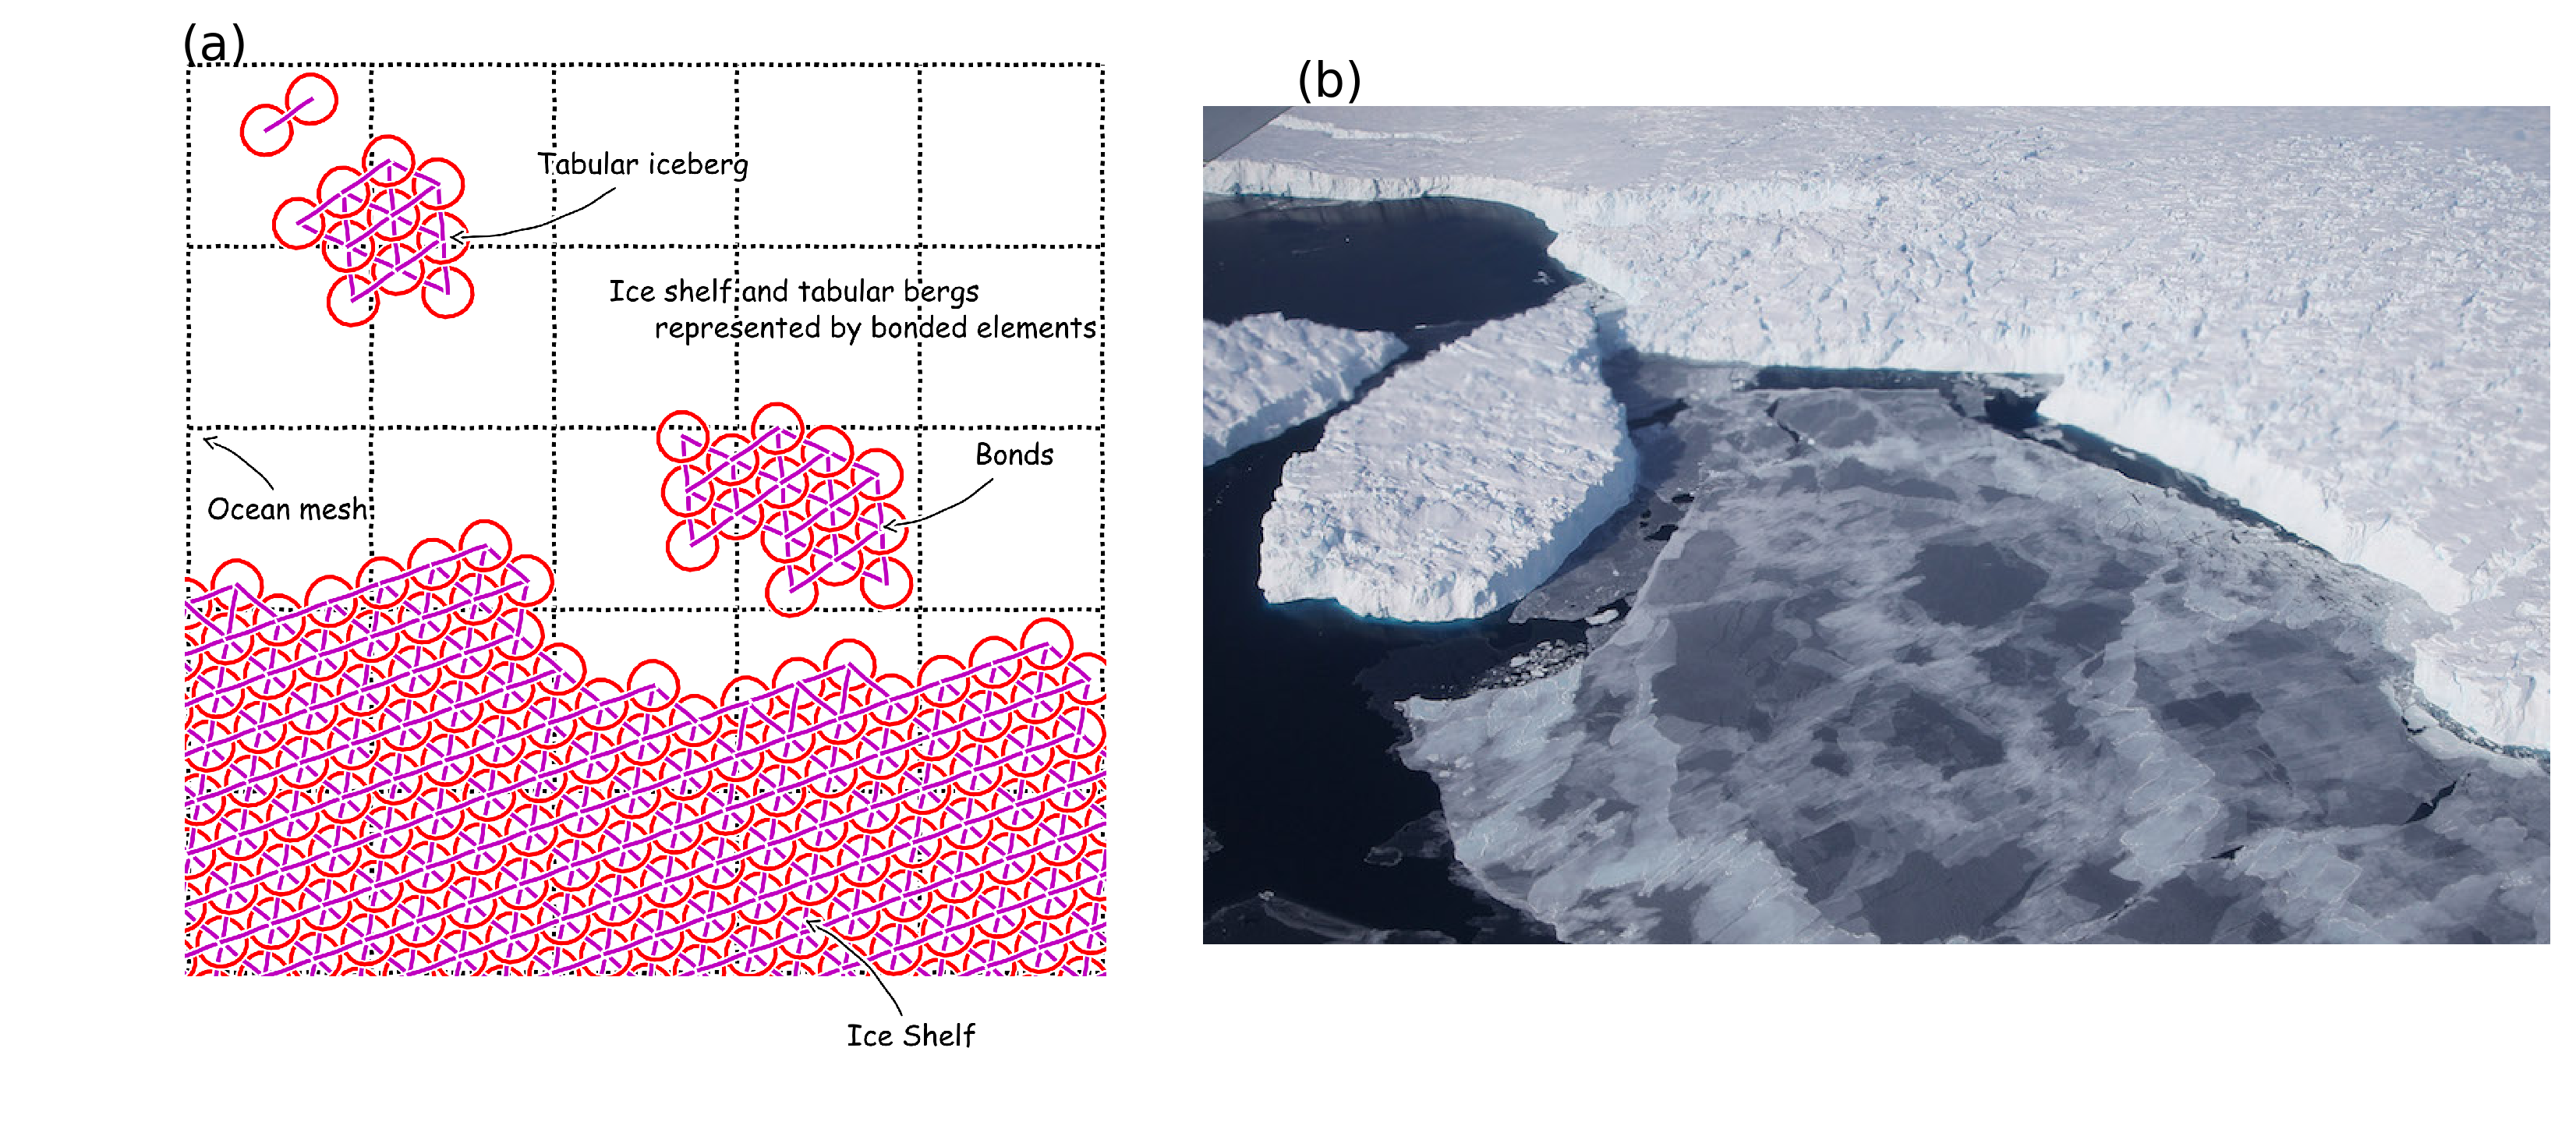
\includegraphics[width=0.99\textwidth]{Figures/Two_panel_schematic_shelf.png}
\caption{ {Schematic showing how ice shelves and tabular icebergs are constructed using Lagrangian elements. 
(a) Schematic of multiple ice elements that are joined together by numerical bonds (magenta lines) to form larger structures such as ice shelves and tabular icebergs. These numerical elements have finite extent and are able to interact with the ocean across multiple grid cells, and can interact with other elements. (b) Areal photograph of an ice shelf and tabular iceberg with elements superimposed over it to illustrate how the Lagrangian elements can be used to model ice shelves and tabular icebergs. In this schematic the ice elements (purple dots) are initialized in a staggered lattice covering the surface area of the iceberg. For the purpose of mass aggregation, the ice elements are assumed to have hexagonal shape (red hexagons). For the purpose of element interactions, the ice elements are assumed to be circular (black circles). Elements are initially bonded to adjacent elements using numerical bonds (magenta lines). These numerical bonds form equilateral triangles which give the shape rigidity. An ocean grid has been included (dashed cyan lines). 
\textcolor{red}{Still need to update this figure to include the super imposed hexagons. Also, perhaps we want to remove some of the text in the caption? (e.g.: remove from the words "In this schematic the ice elements").}
%The background photo in the larger schematic is an areal photograph of iceberg PIIB (Area= 42 $\textrm{km}^{2}$) taken in Baffin Bay in 2012. The red ship can be identified on the bottom of the photo for scale. 
%Schematic showing how Lagrangian elements are used when modeling tabular icebergs. Lagrangian elements (blue dots) are initialized in a staggered lattice covering the surface area of the iceberg. For purposed of mass aggregation, the ice elements are assumed to have hexagonal shape (grey hexagons). For purposed of element interactions, the ice elements are assumed to be circular (black circles). Elements are initially bonded to adjacent elements using numerical bonds (dashed white lines). These numerical bonds form equilateral triangles which give the shape rigidity. 
%The inset panel shows a schematic of the intersection of a hexagonal element and the ocean grid. The colors indicate the fraction of the hexagon that lies in each grid cell. These fractions are used as weights to spread iceberg model properties to the ocean grid (see text for more details).
}}
\end{center}
\label{fig:Schematic}
\end{figure}
 \clearpage


%\begin{figure}
%\begin{center}
%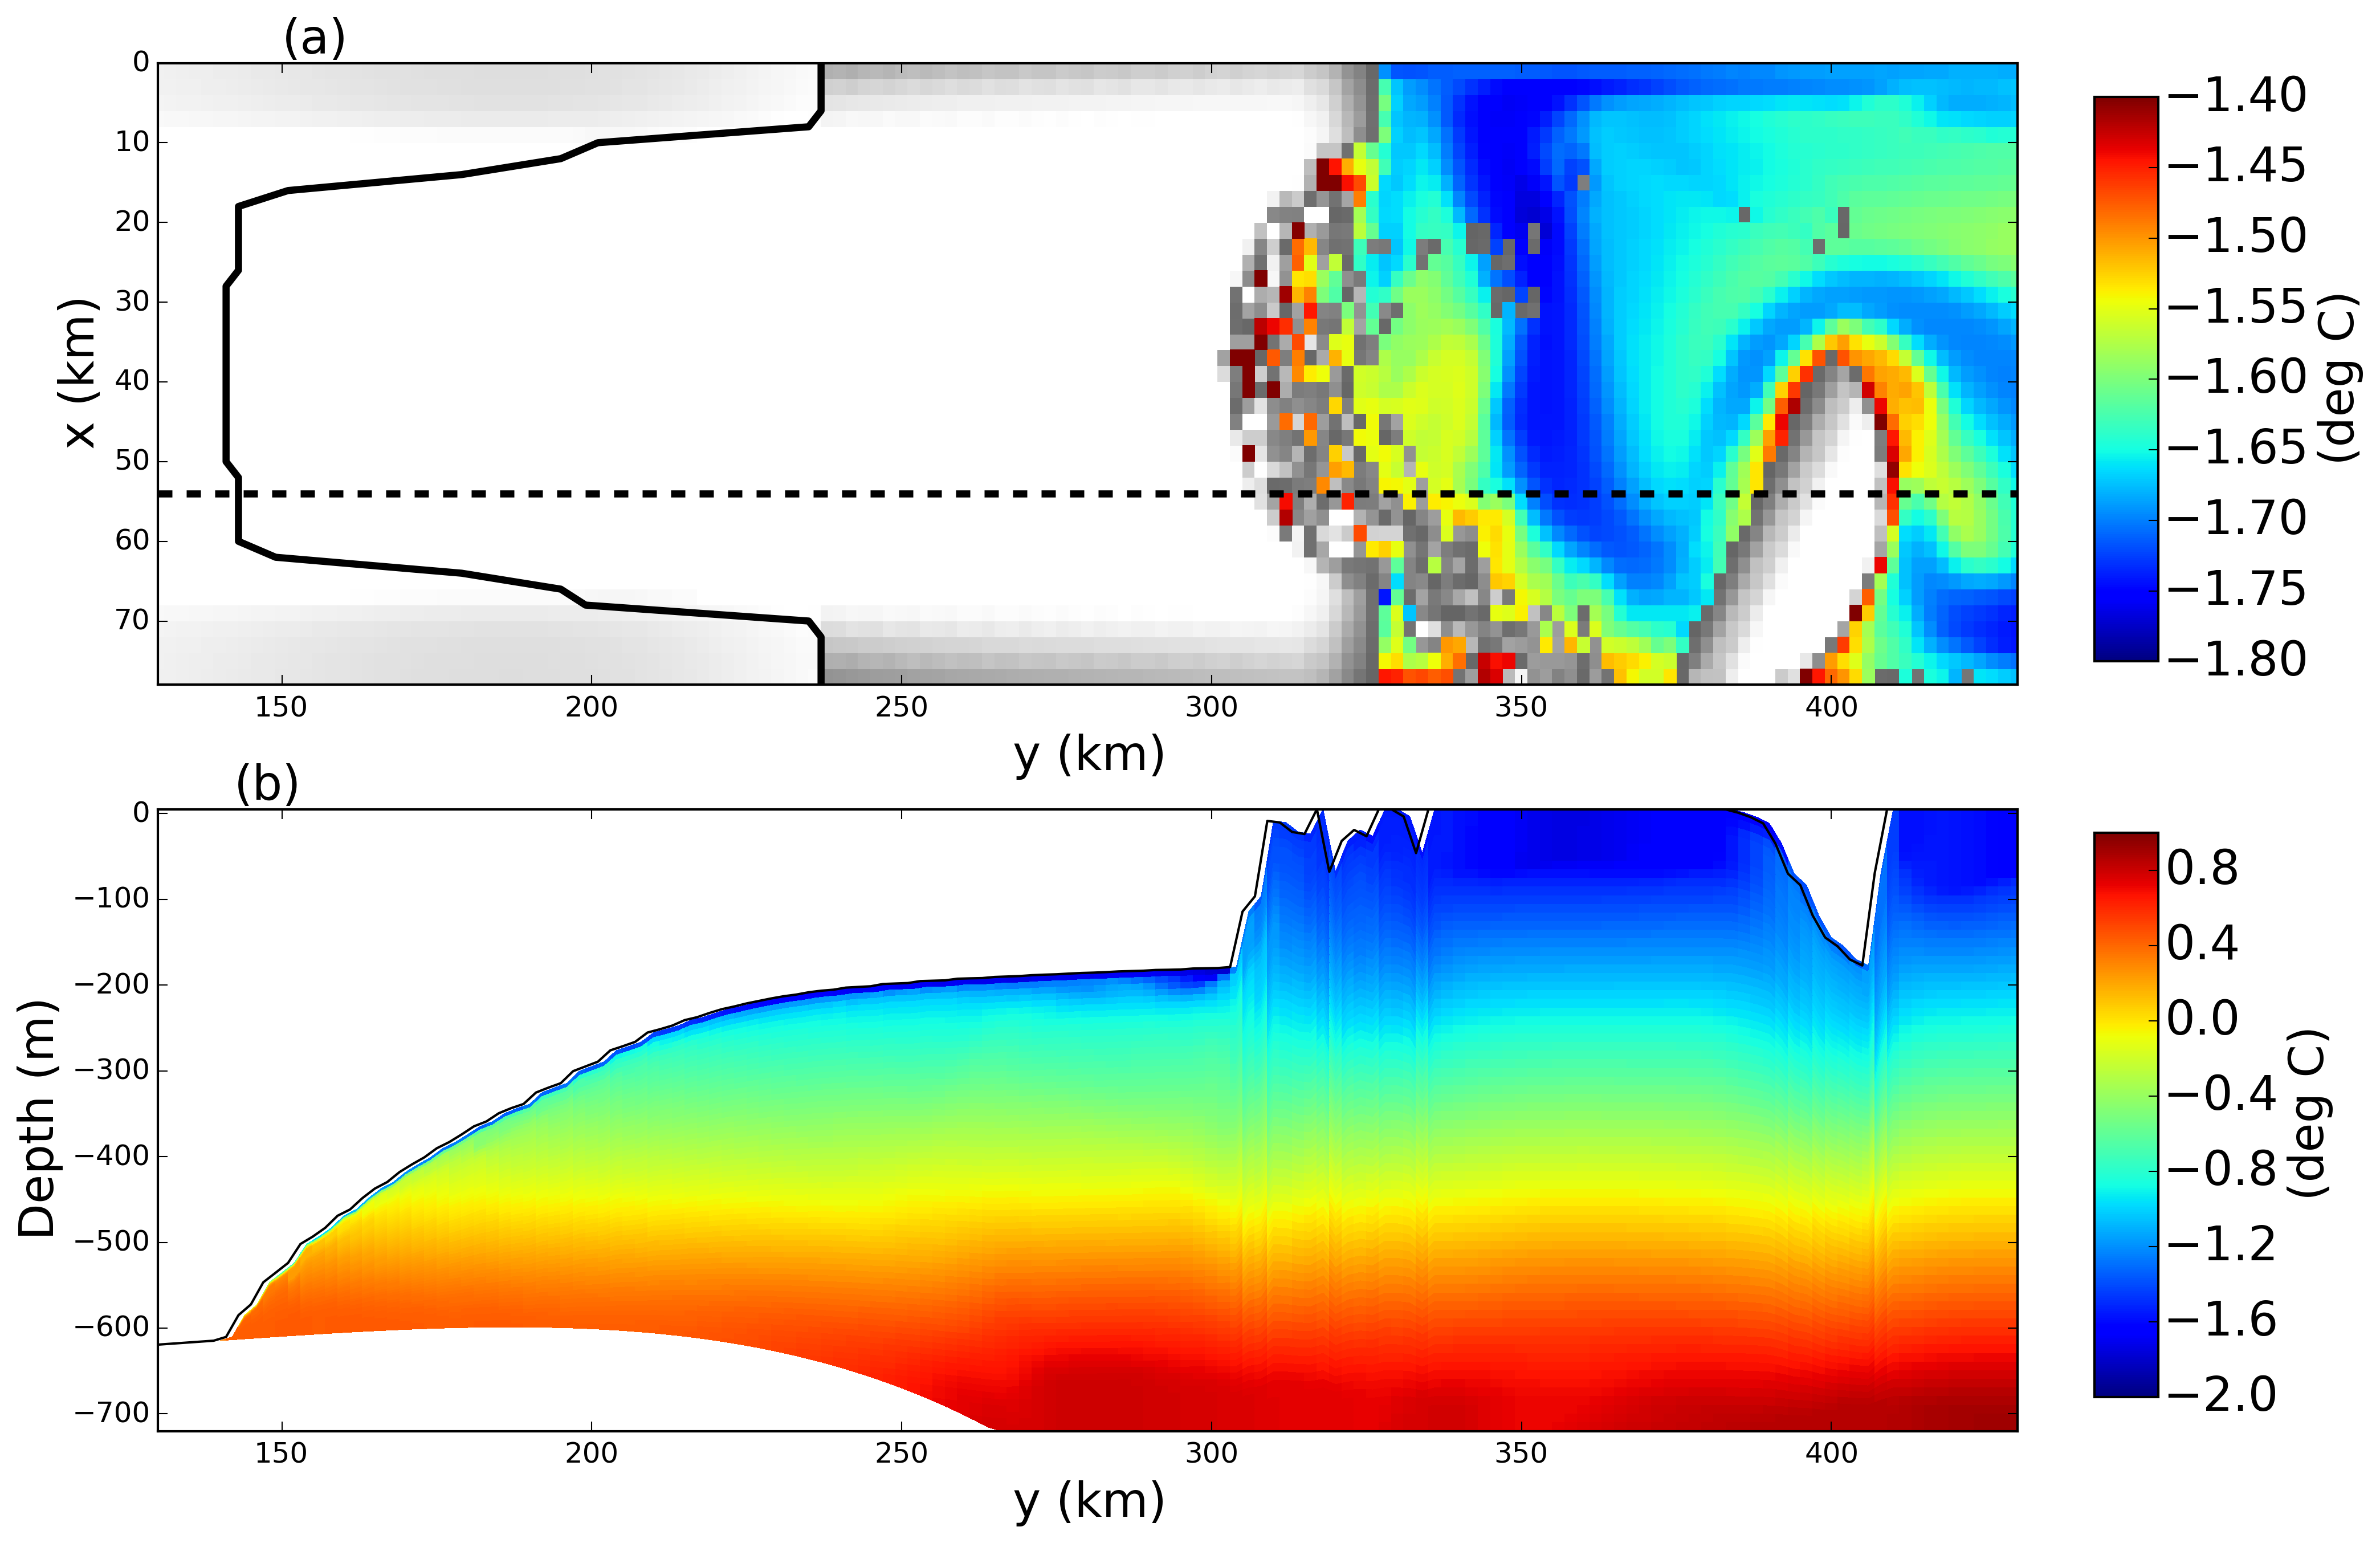
\includegraphics[width=0.99\textwidth]{Figures/side_and_top_view_ALE_z_Mixed_Melt_Collapse_temp_layers_x12.png}
%\caption{ {Snapshots of a simulation where a Lagrangian ice-shelf calves a tabular iceberg viewed (a) from above and (b) from the side. The snapshots is taken 30 days after calving. Panel (a) shows the sea surface temperature. Grid cells with ice mass $>10^{4}$ kg are plotted in white, with grey shading indicating thinner ice. Panel (b) shows a vertical sections of ocean temperature at $x$=54~km. The position of the vertical section is shown by the dashed line in panel (a). The solid line in panel (a) shows the position of the grounding line.}}
%\end{center}
%\label{fig:Iceberg_calving}
%\end{figure}
% \clearpage


\begin{figure}
\begin{center}
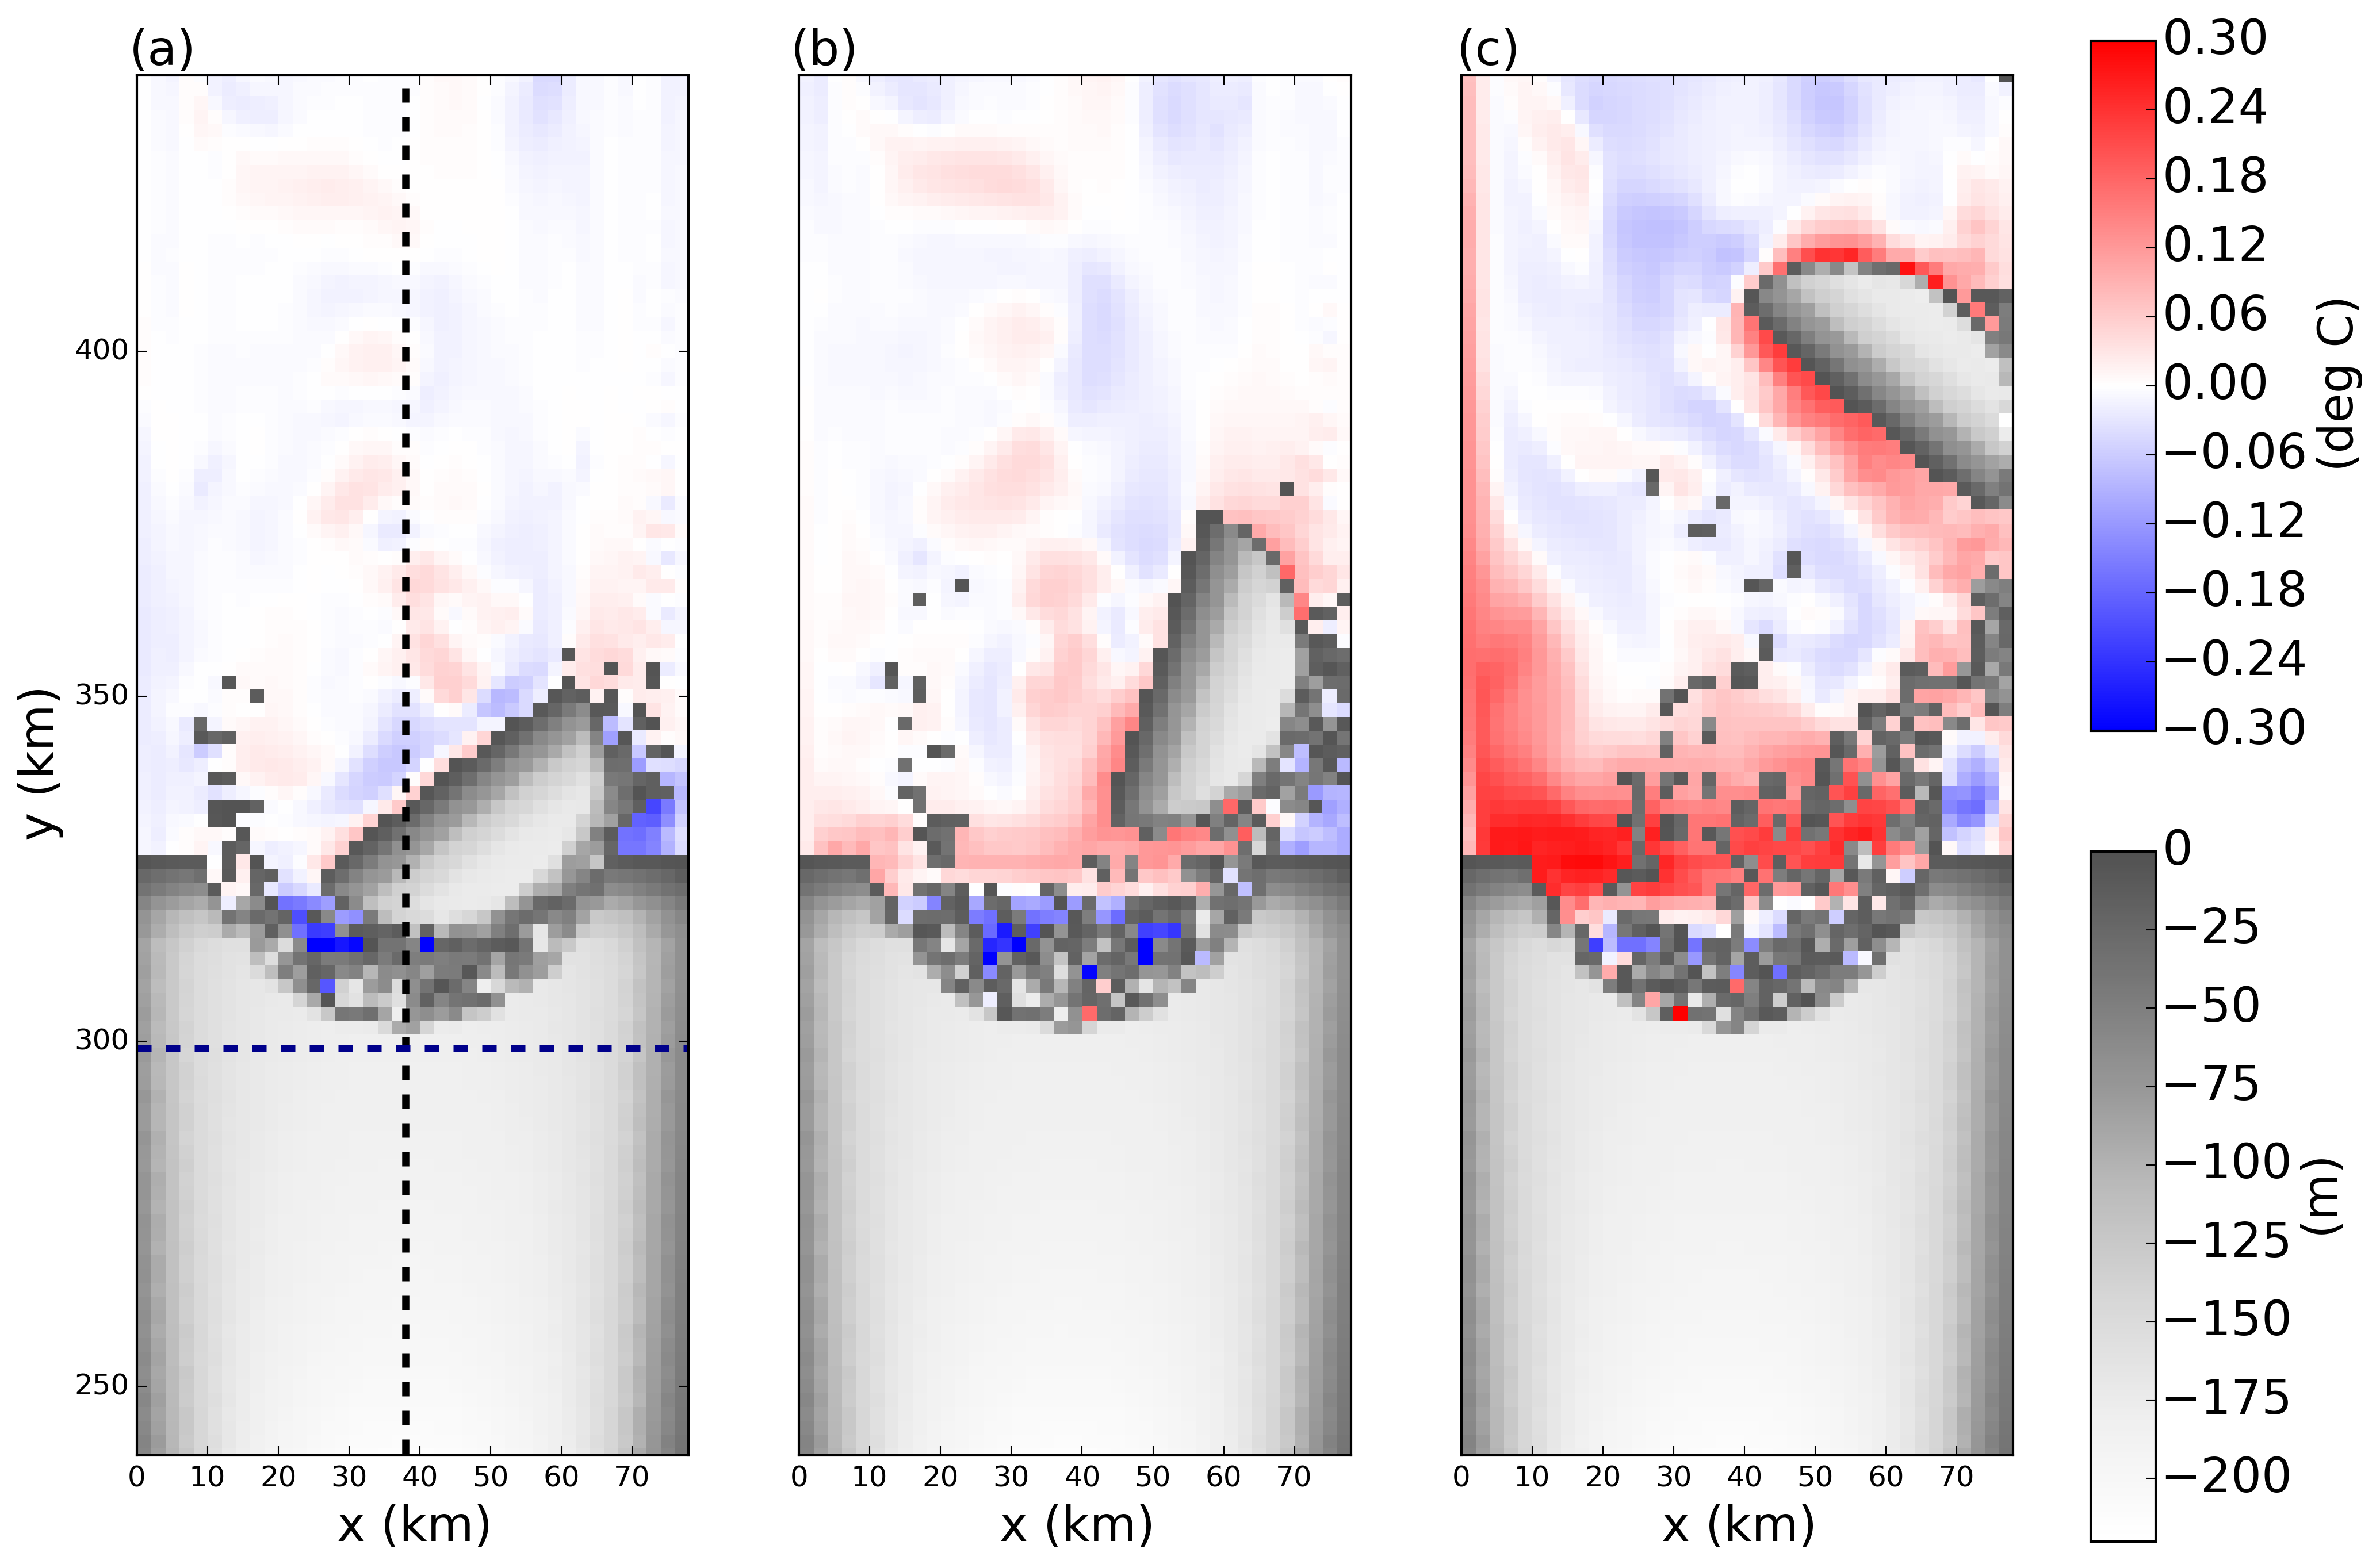
\includegraphics[width=0.99\textwidth]{Figures/snapshots_Wind_Wind_Collapse_temp_anomaly.png}
\caption{ {Snapshots of sea surface temperature anomalies in the iceberg-calving simulation. The anomalies are relative to pre-calving temperatures. Snapshots are taken (a) 7, (b) 15, and (c) 50 days after calving. Grid cells with ice mass $> 10^{4}$ kg are plotted in white, with grey shading indicating thinner ice.  The black and blue dashed line in panel (a) shows the location of the vertical transects shown in Figures \ref{fig:Temperature_section_Collapse_yz} and \ref{fig:v_velocity_vertical}, and \ref{fig:Temperature_section_Collapse_xz}, respectively.}}
\end{center}
%FIgure created by \end{center}
\label{fig:SST_snapshots}
\end{figure}
 \clearpage



\begin{figure}
\begin{center}
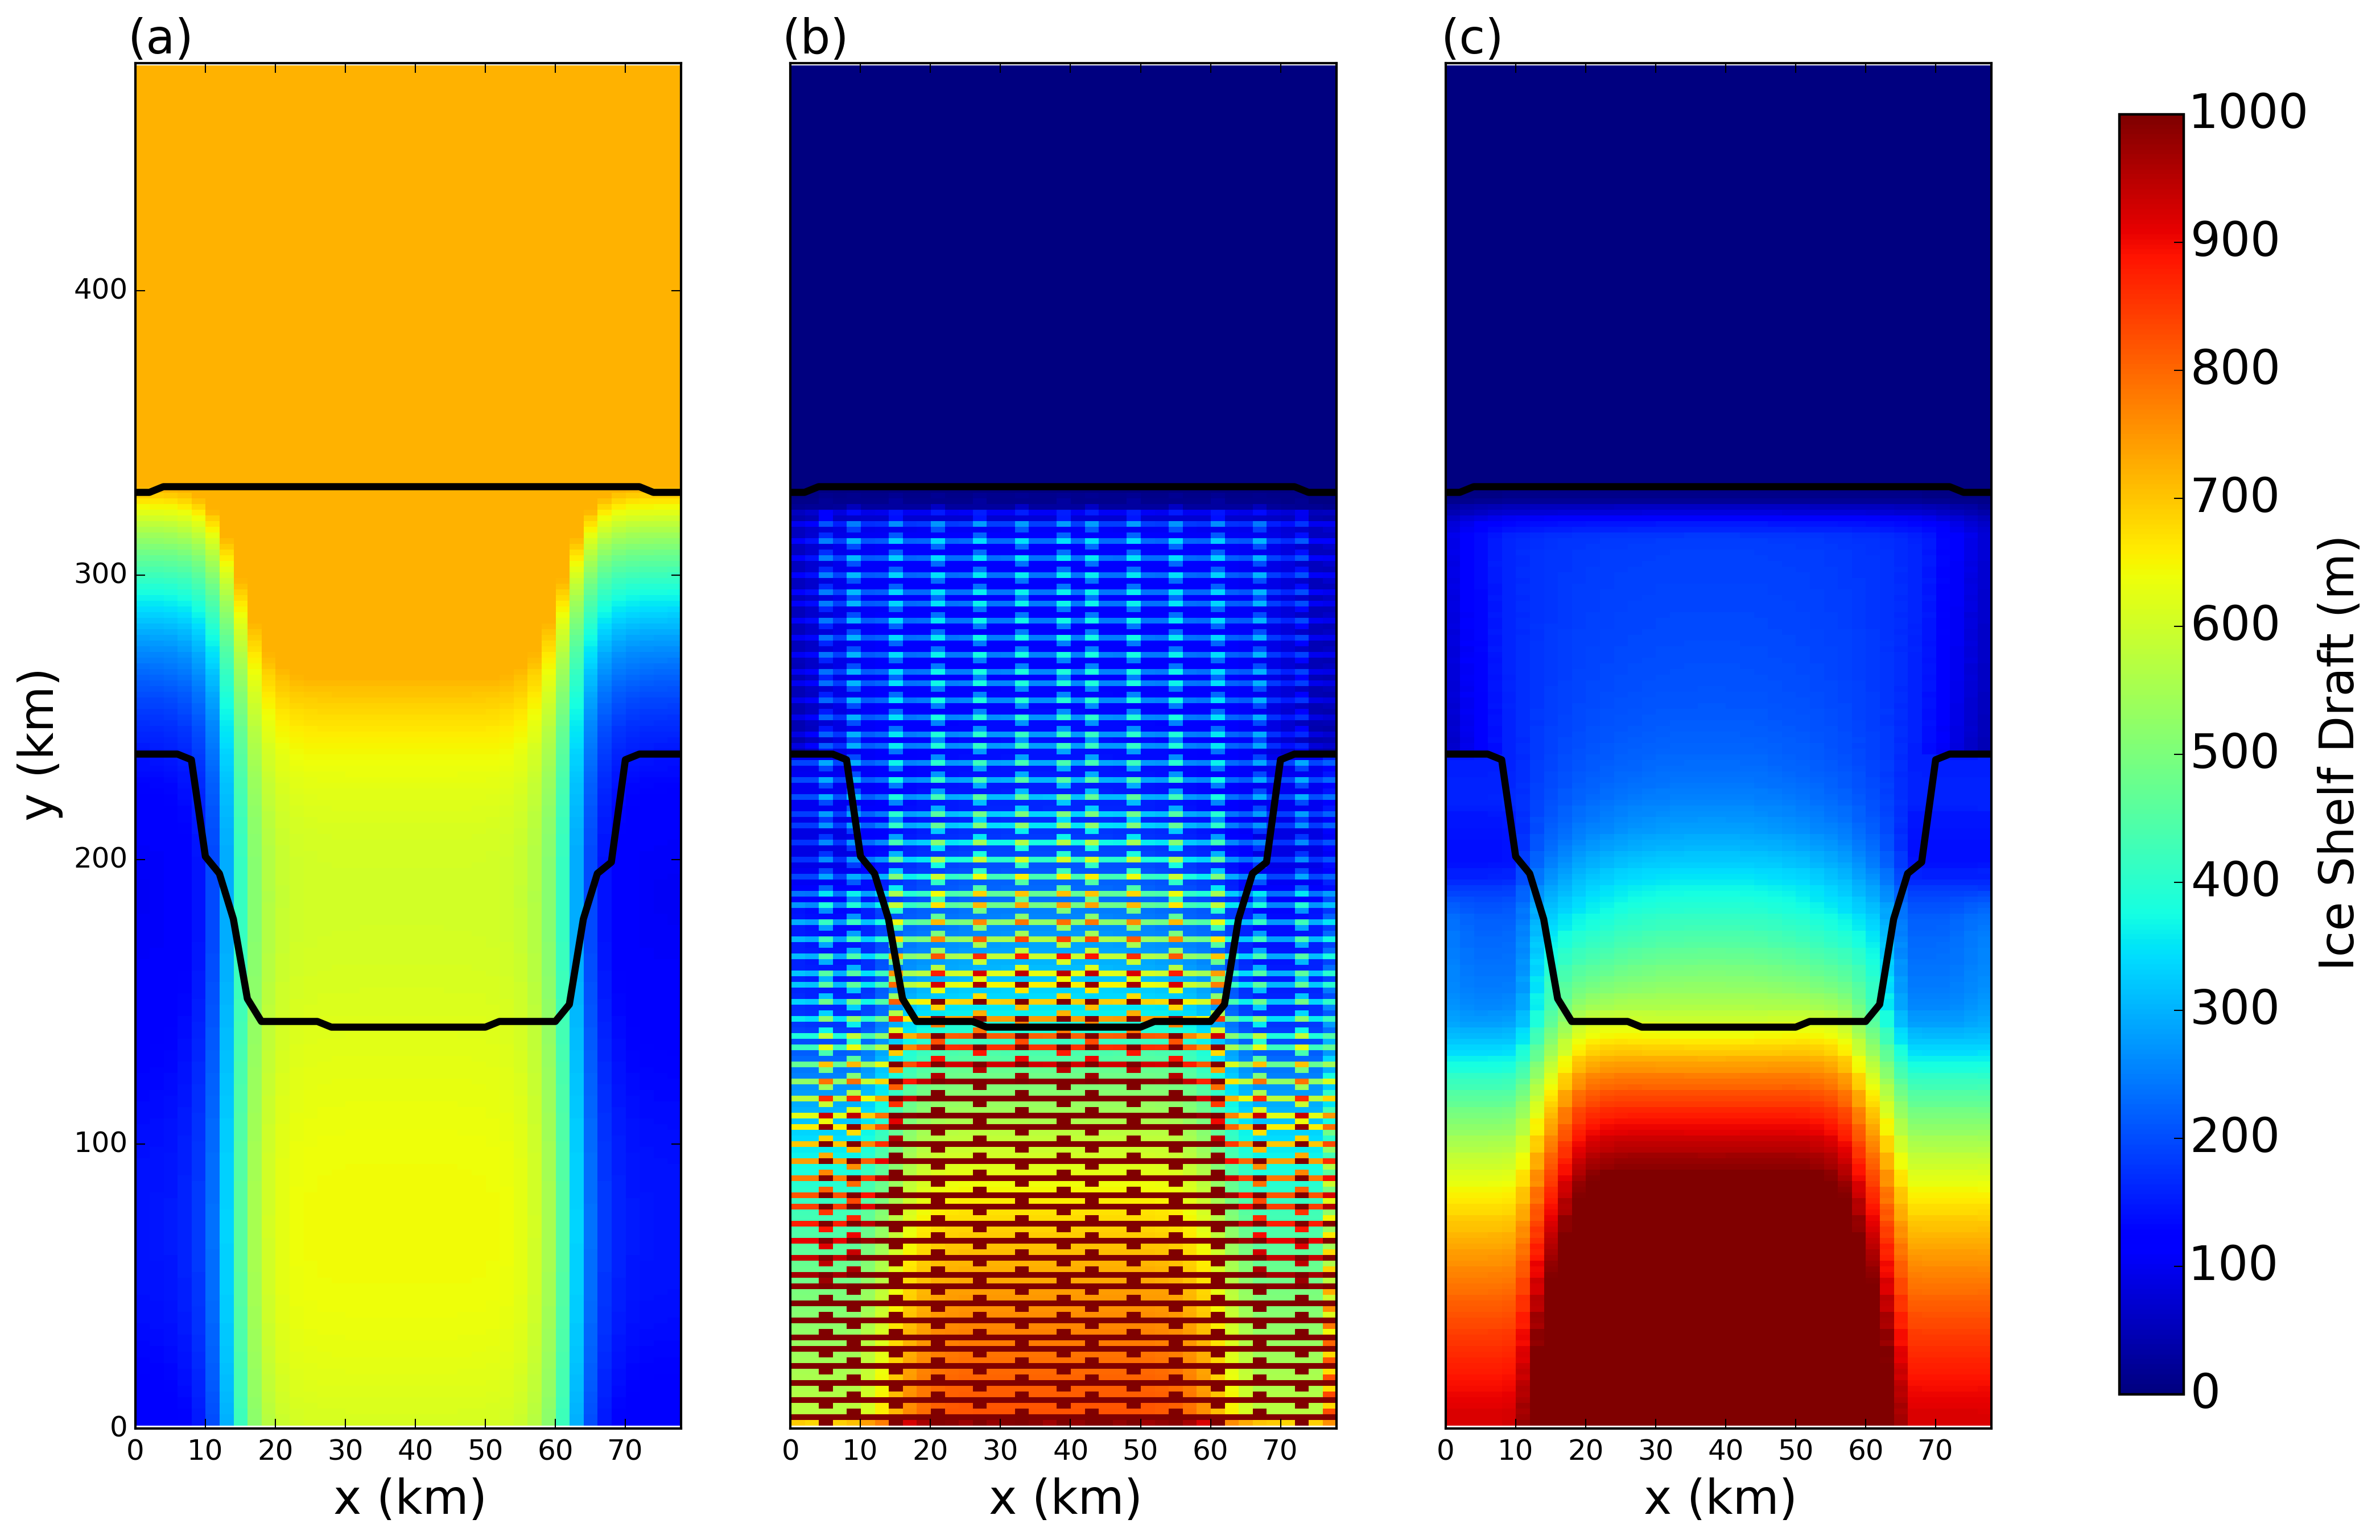
\includegraphics[width=0.99\textwidth]{Figures/ALE_z_static_shelf_solo_D_mass_spread_mass.png}
\caption{ {(a) Ocean bottom topography and (c) ice-shelf draft used to initialized the static ice shelf experiment simulation. The ice draft is calculated from the total mass of ice intersecting each ocean grid cell (see Section 2.6). Panel (b) shows the initial ice draft that would be calculated if the mass aggregation onto the Eularian grid was not used (i.e. elements treated as point masses). The lower and upper black lines denote the grounding line and ice shelf front, respectively. This figure is reproduced from \citep{Stern2017}. } \label{fig:ISOMIP_mass_and_topog}}
\end{center}
\end{figure}
 \clearpage
 
 

%\begin{figure}
%\begin{center}
%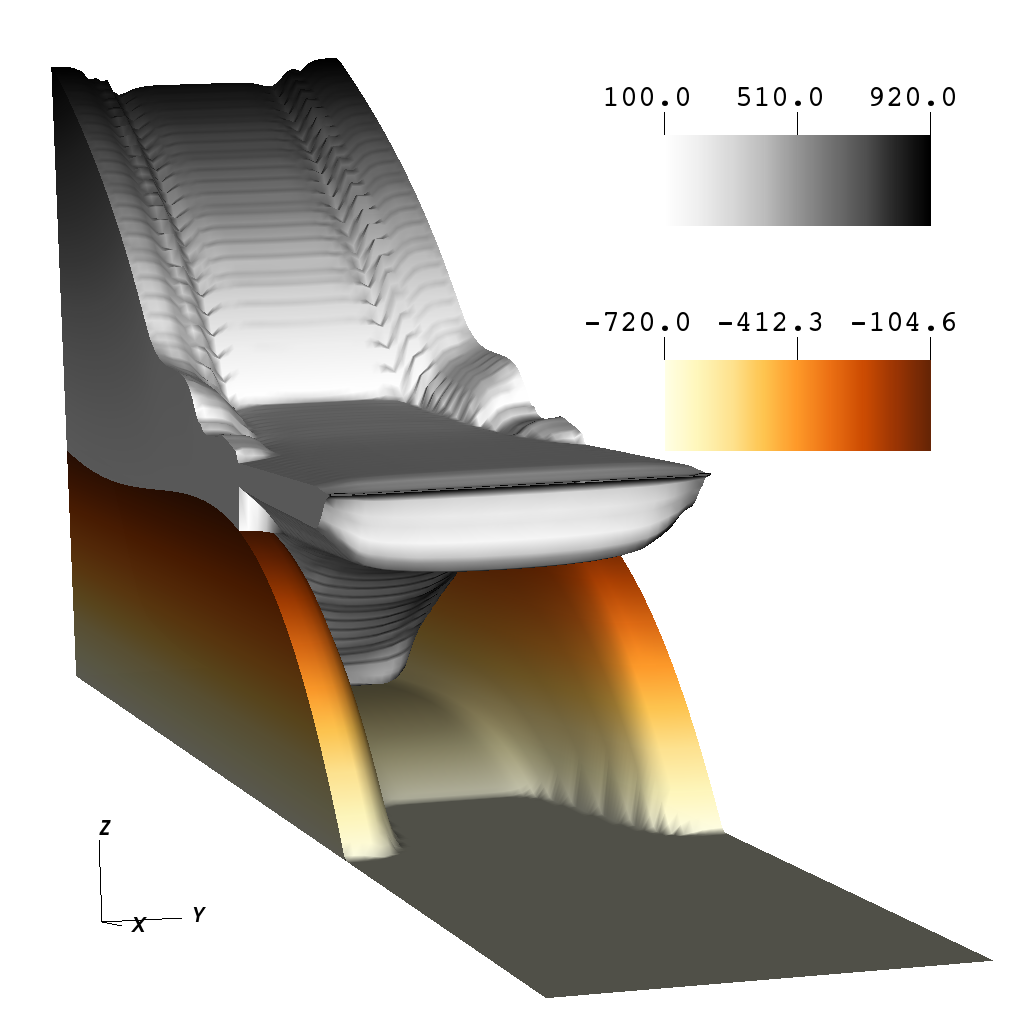
\includegraphics[width=0.99\textwidth]{Figures/Lagrangian_shelf_domain.png}
%\caption{ {Ocean bottom topography and ice-shelf draft used in the Lagrangian and Eulerian static ice-shelf simulations}}
%\end{center}
%\label{fig:ISOMIP_mass_and_topog}
%\end{figure}
% \clearpage
 
 


\begin{figure}
\begin{center}
%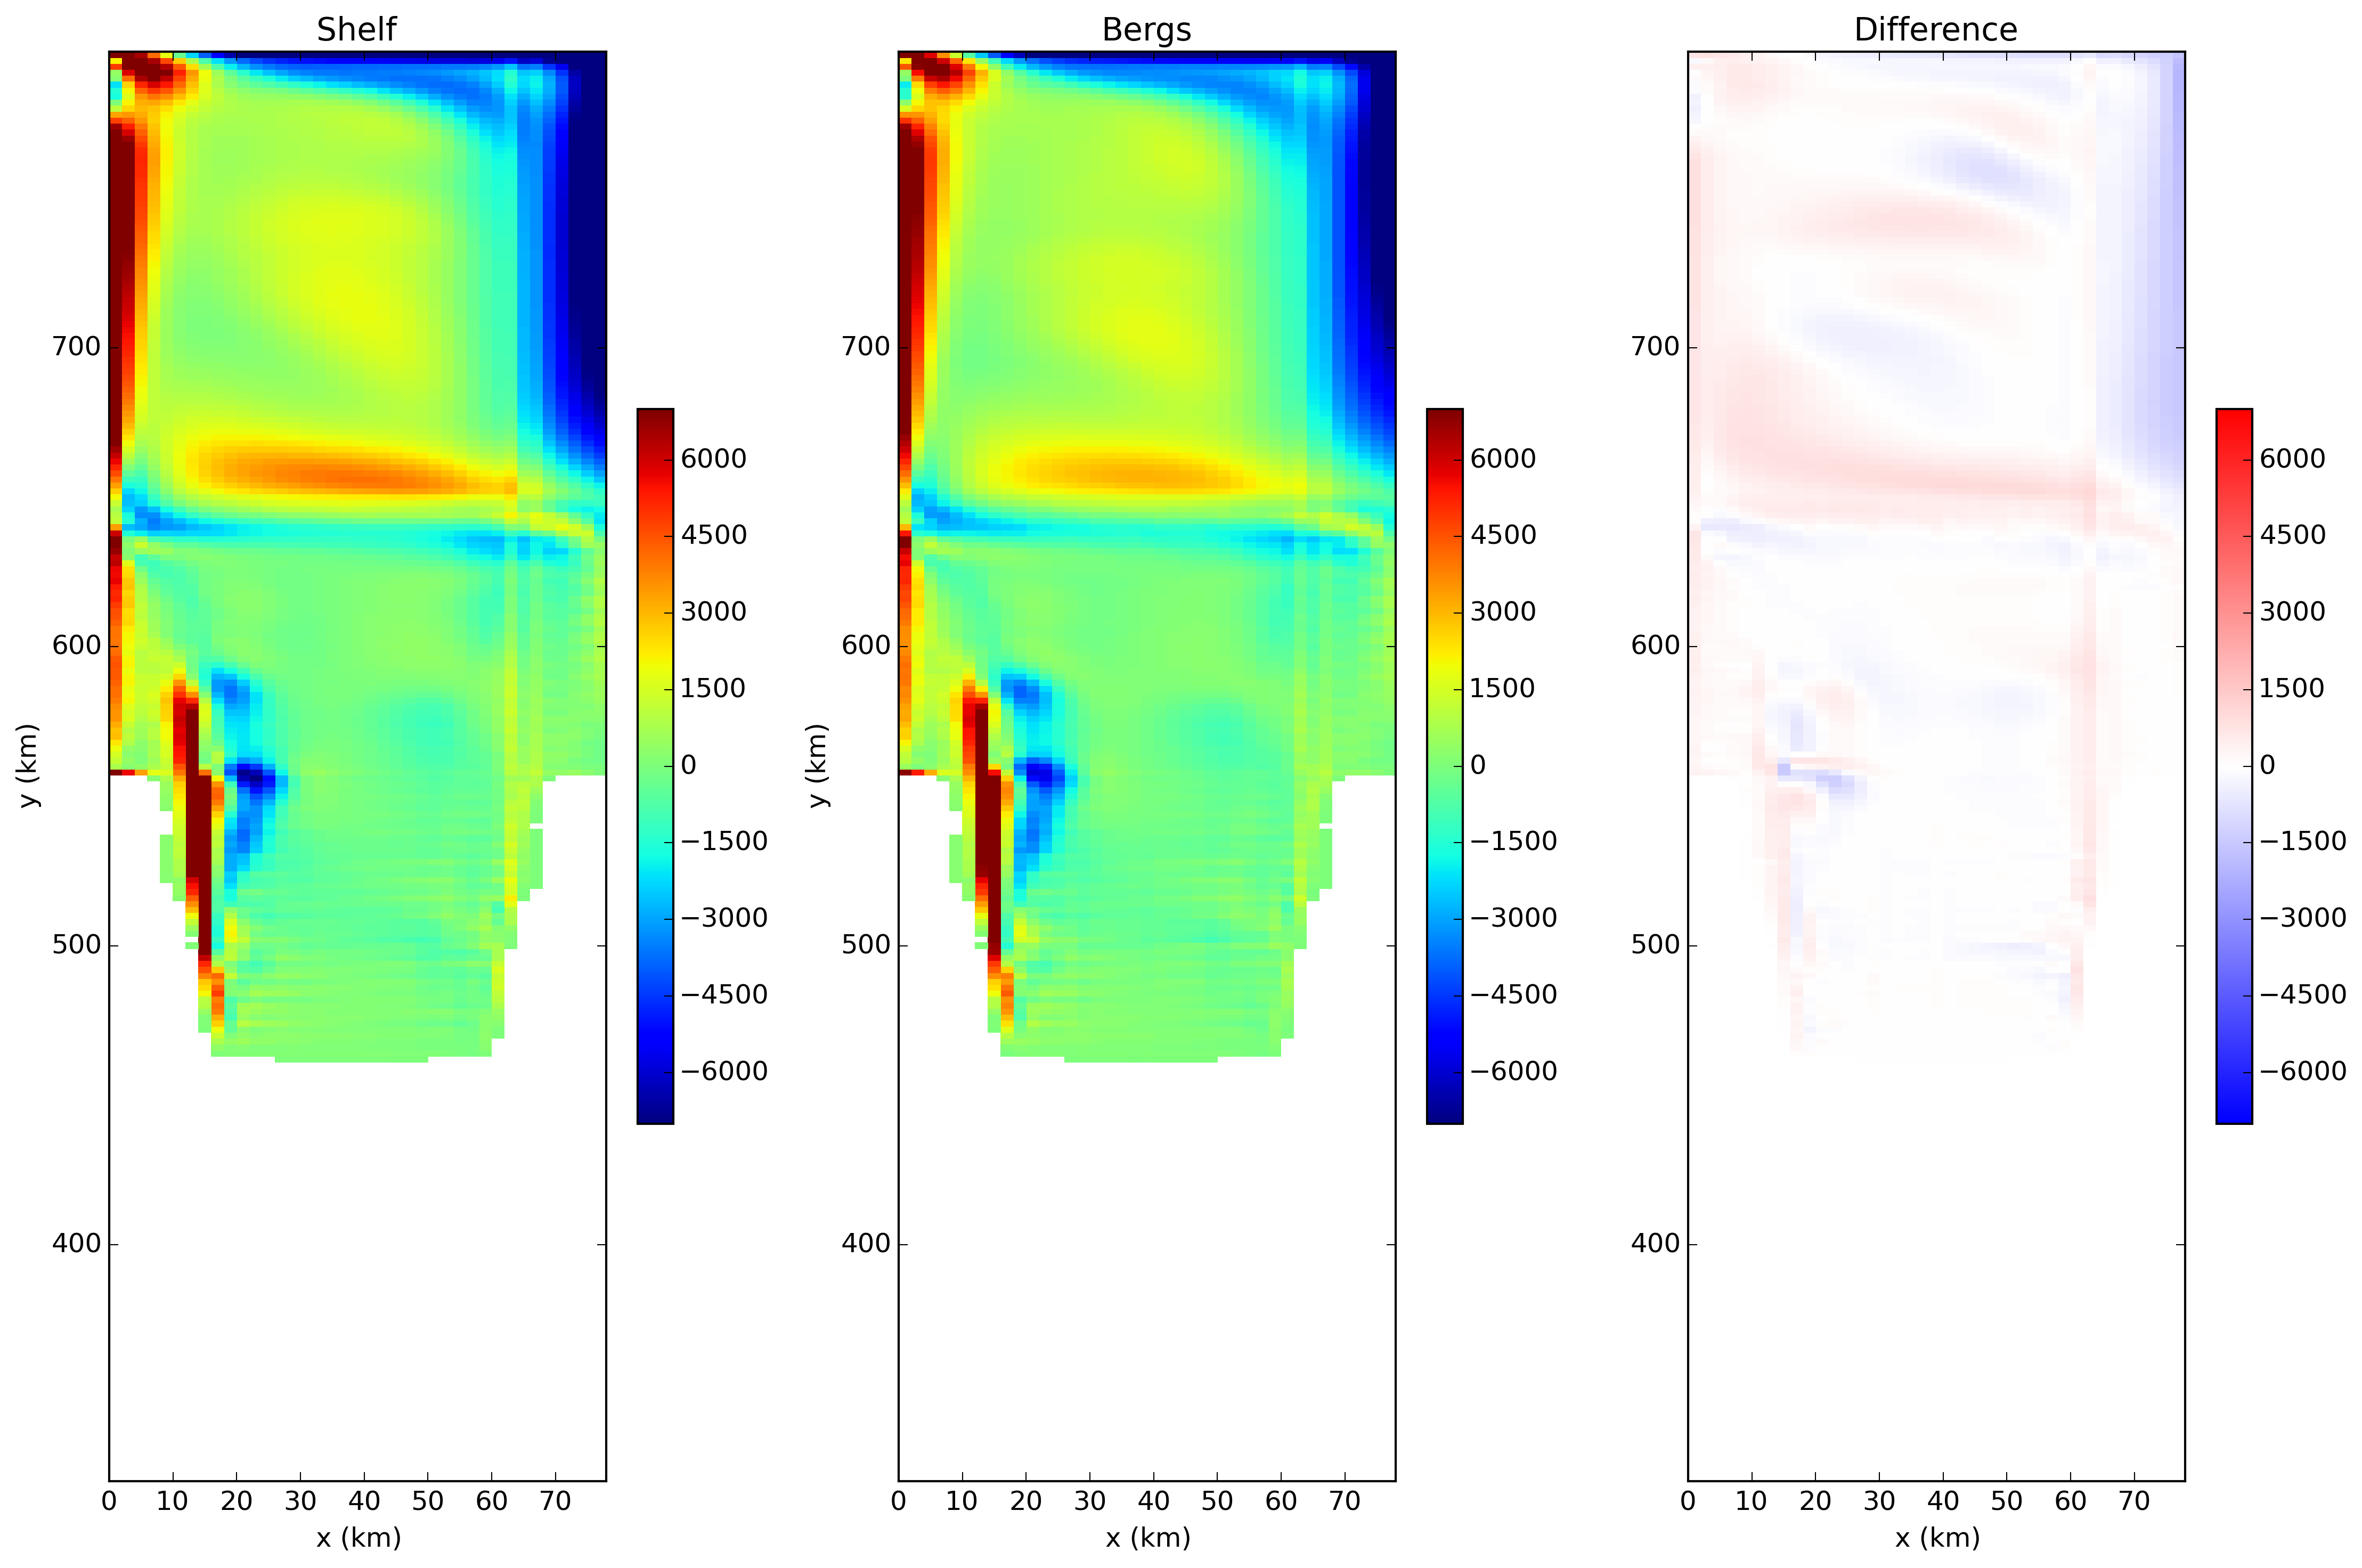
\includegraphics[width=0.99\textwidth]{Figures/ALE_z_static_shelf_comparison_barotropic_sf.png}
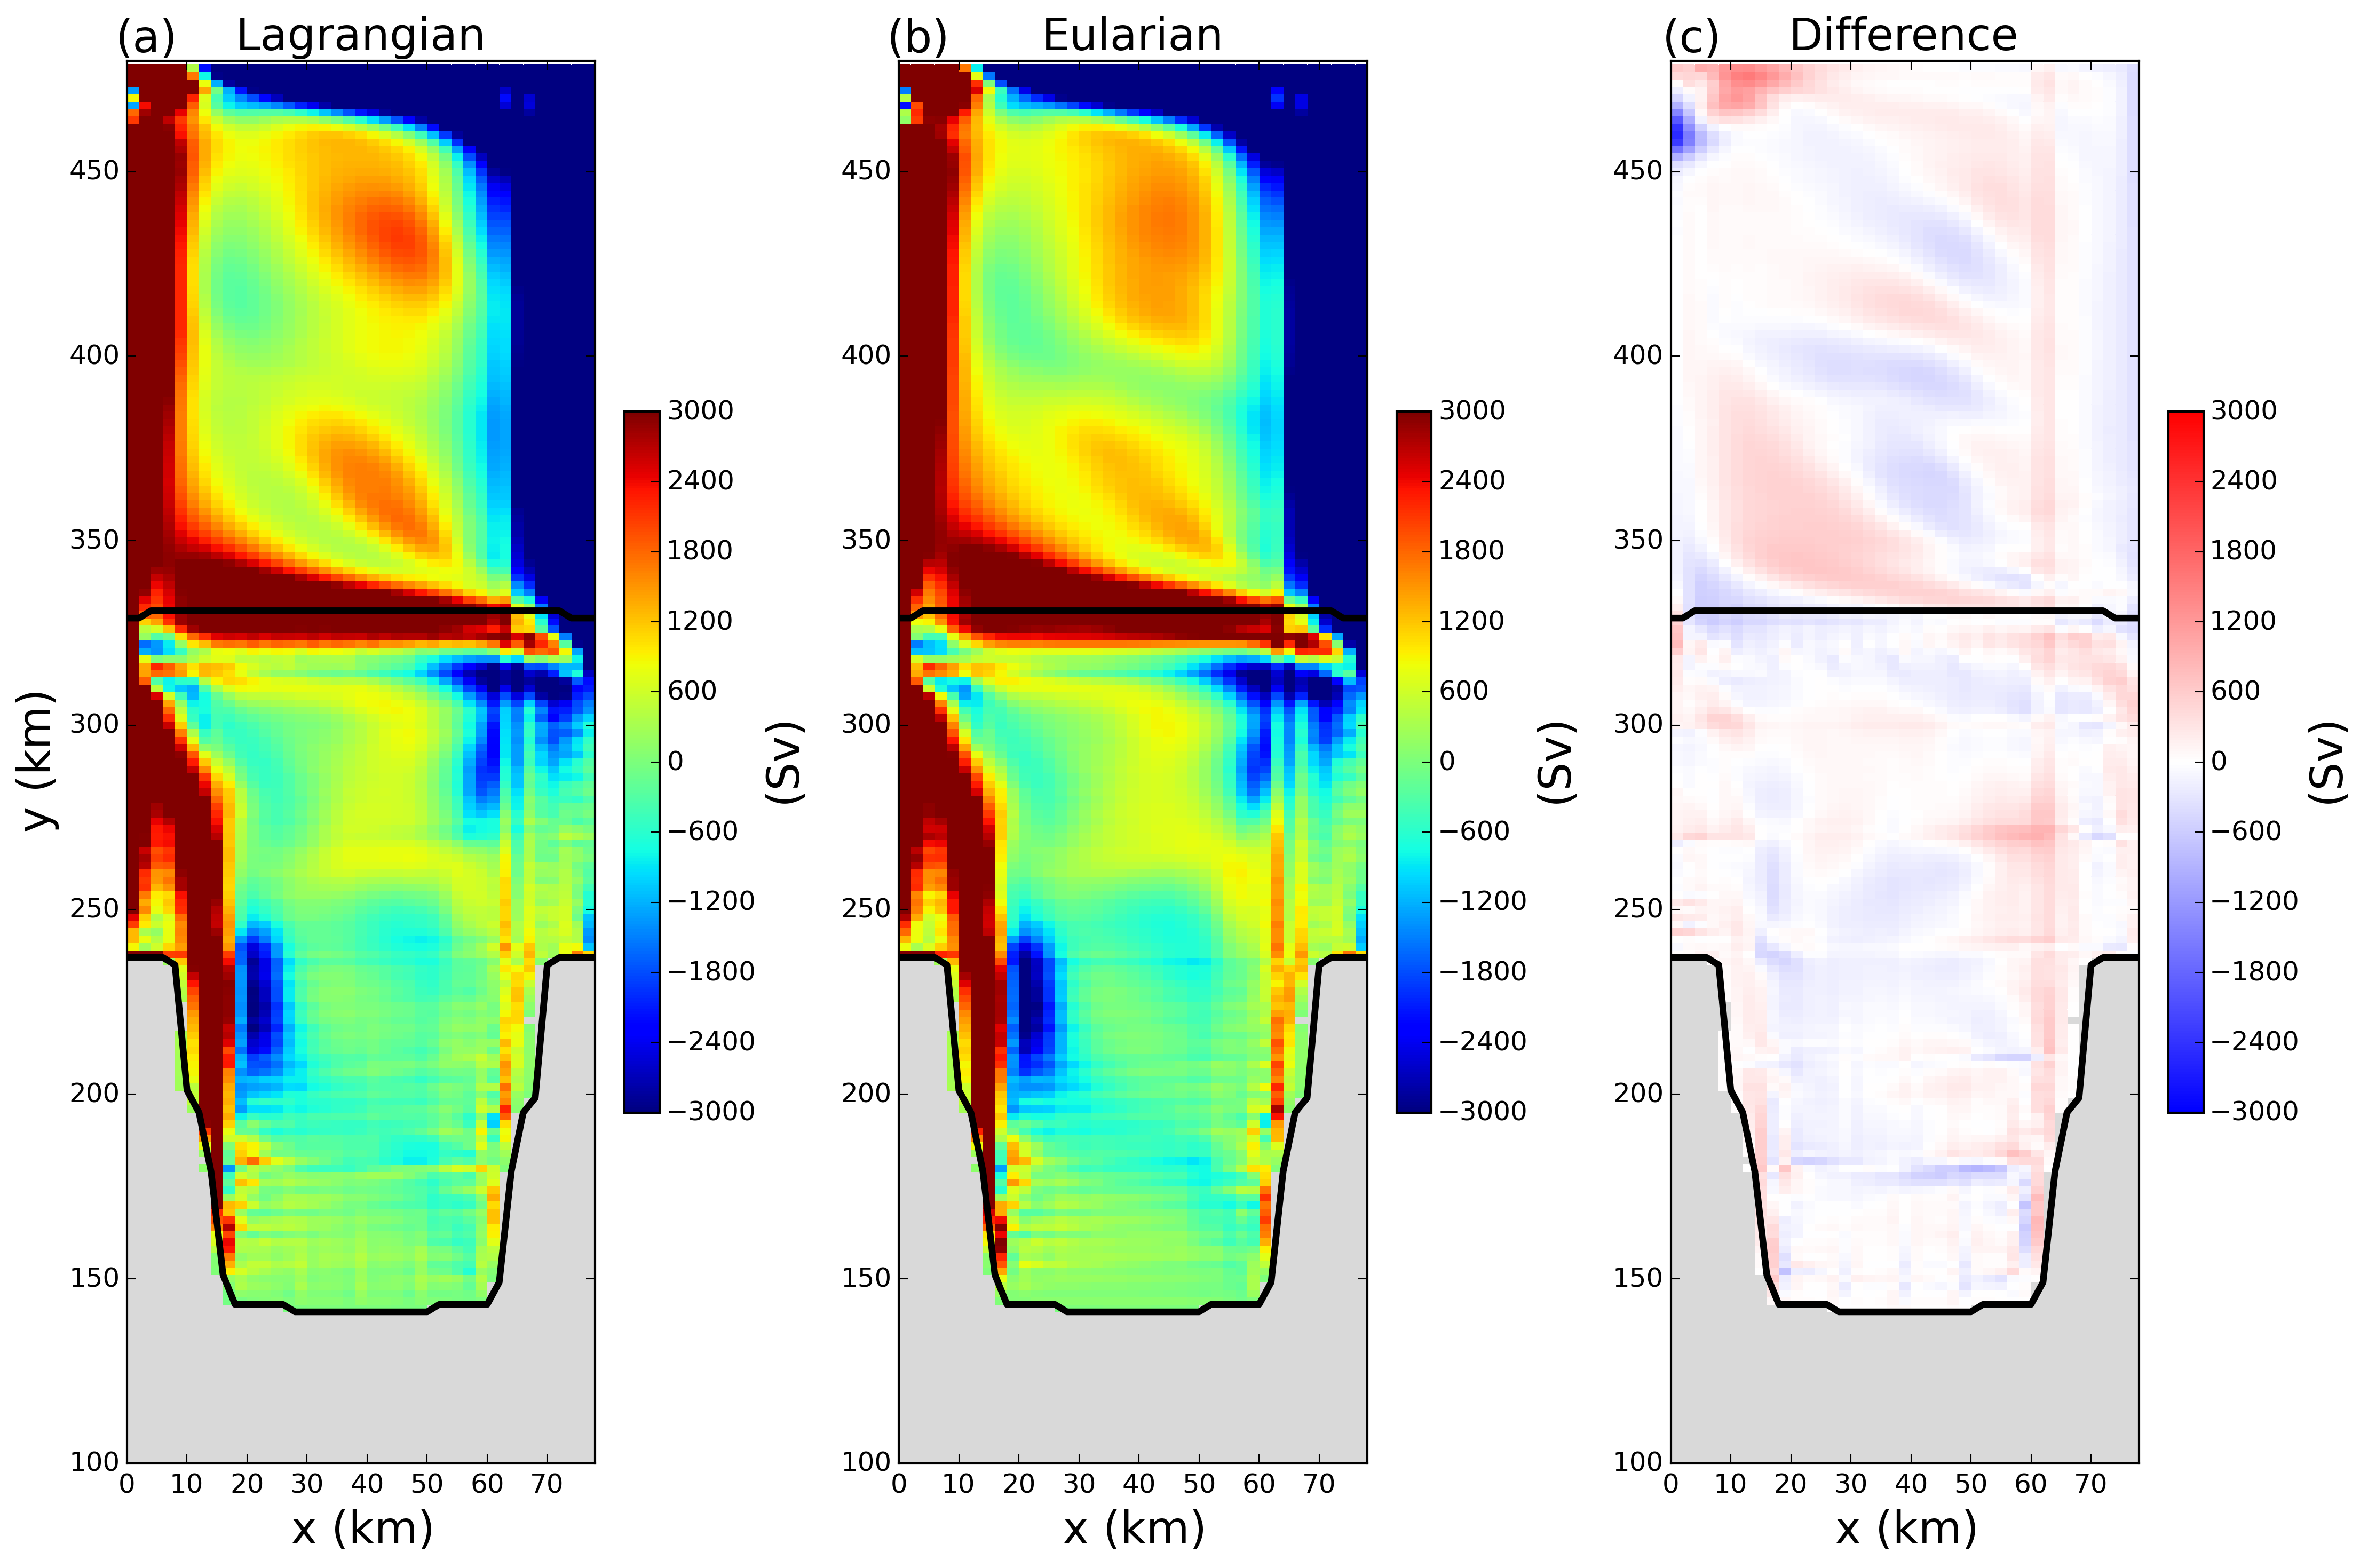
\includegraphics[width=0.99\textwidth]{Figures/Wind_static_shelf_comparison_barotropic_sf.png}
\caption{ {Time-averaged barotropic stream function in the (a) Lagrangian and (b) Eulerian simulations in the static ice-shelf configuration. Panel (c) shows the difference between panels (a) and (b). The time averages are taken over 5 years of model time, beginning at the end of the 5 year spin up period. \textcolor{red}{Something is wrong with the units in this figure}}}
\end{center}
%FIgure created by \end{center}
\label{fig:Bt_comparison}
\end{figure}
 \clearpage



 

\begin{figure}
\begin{center}
%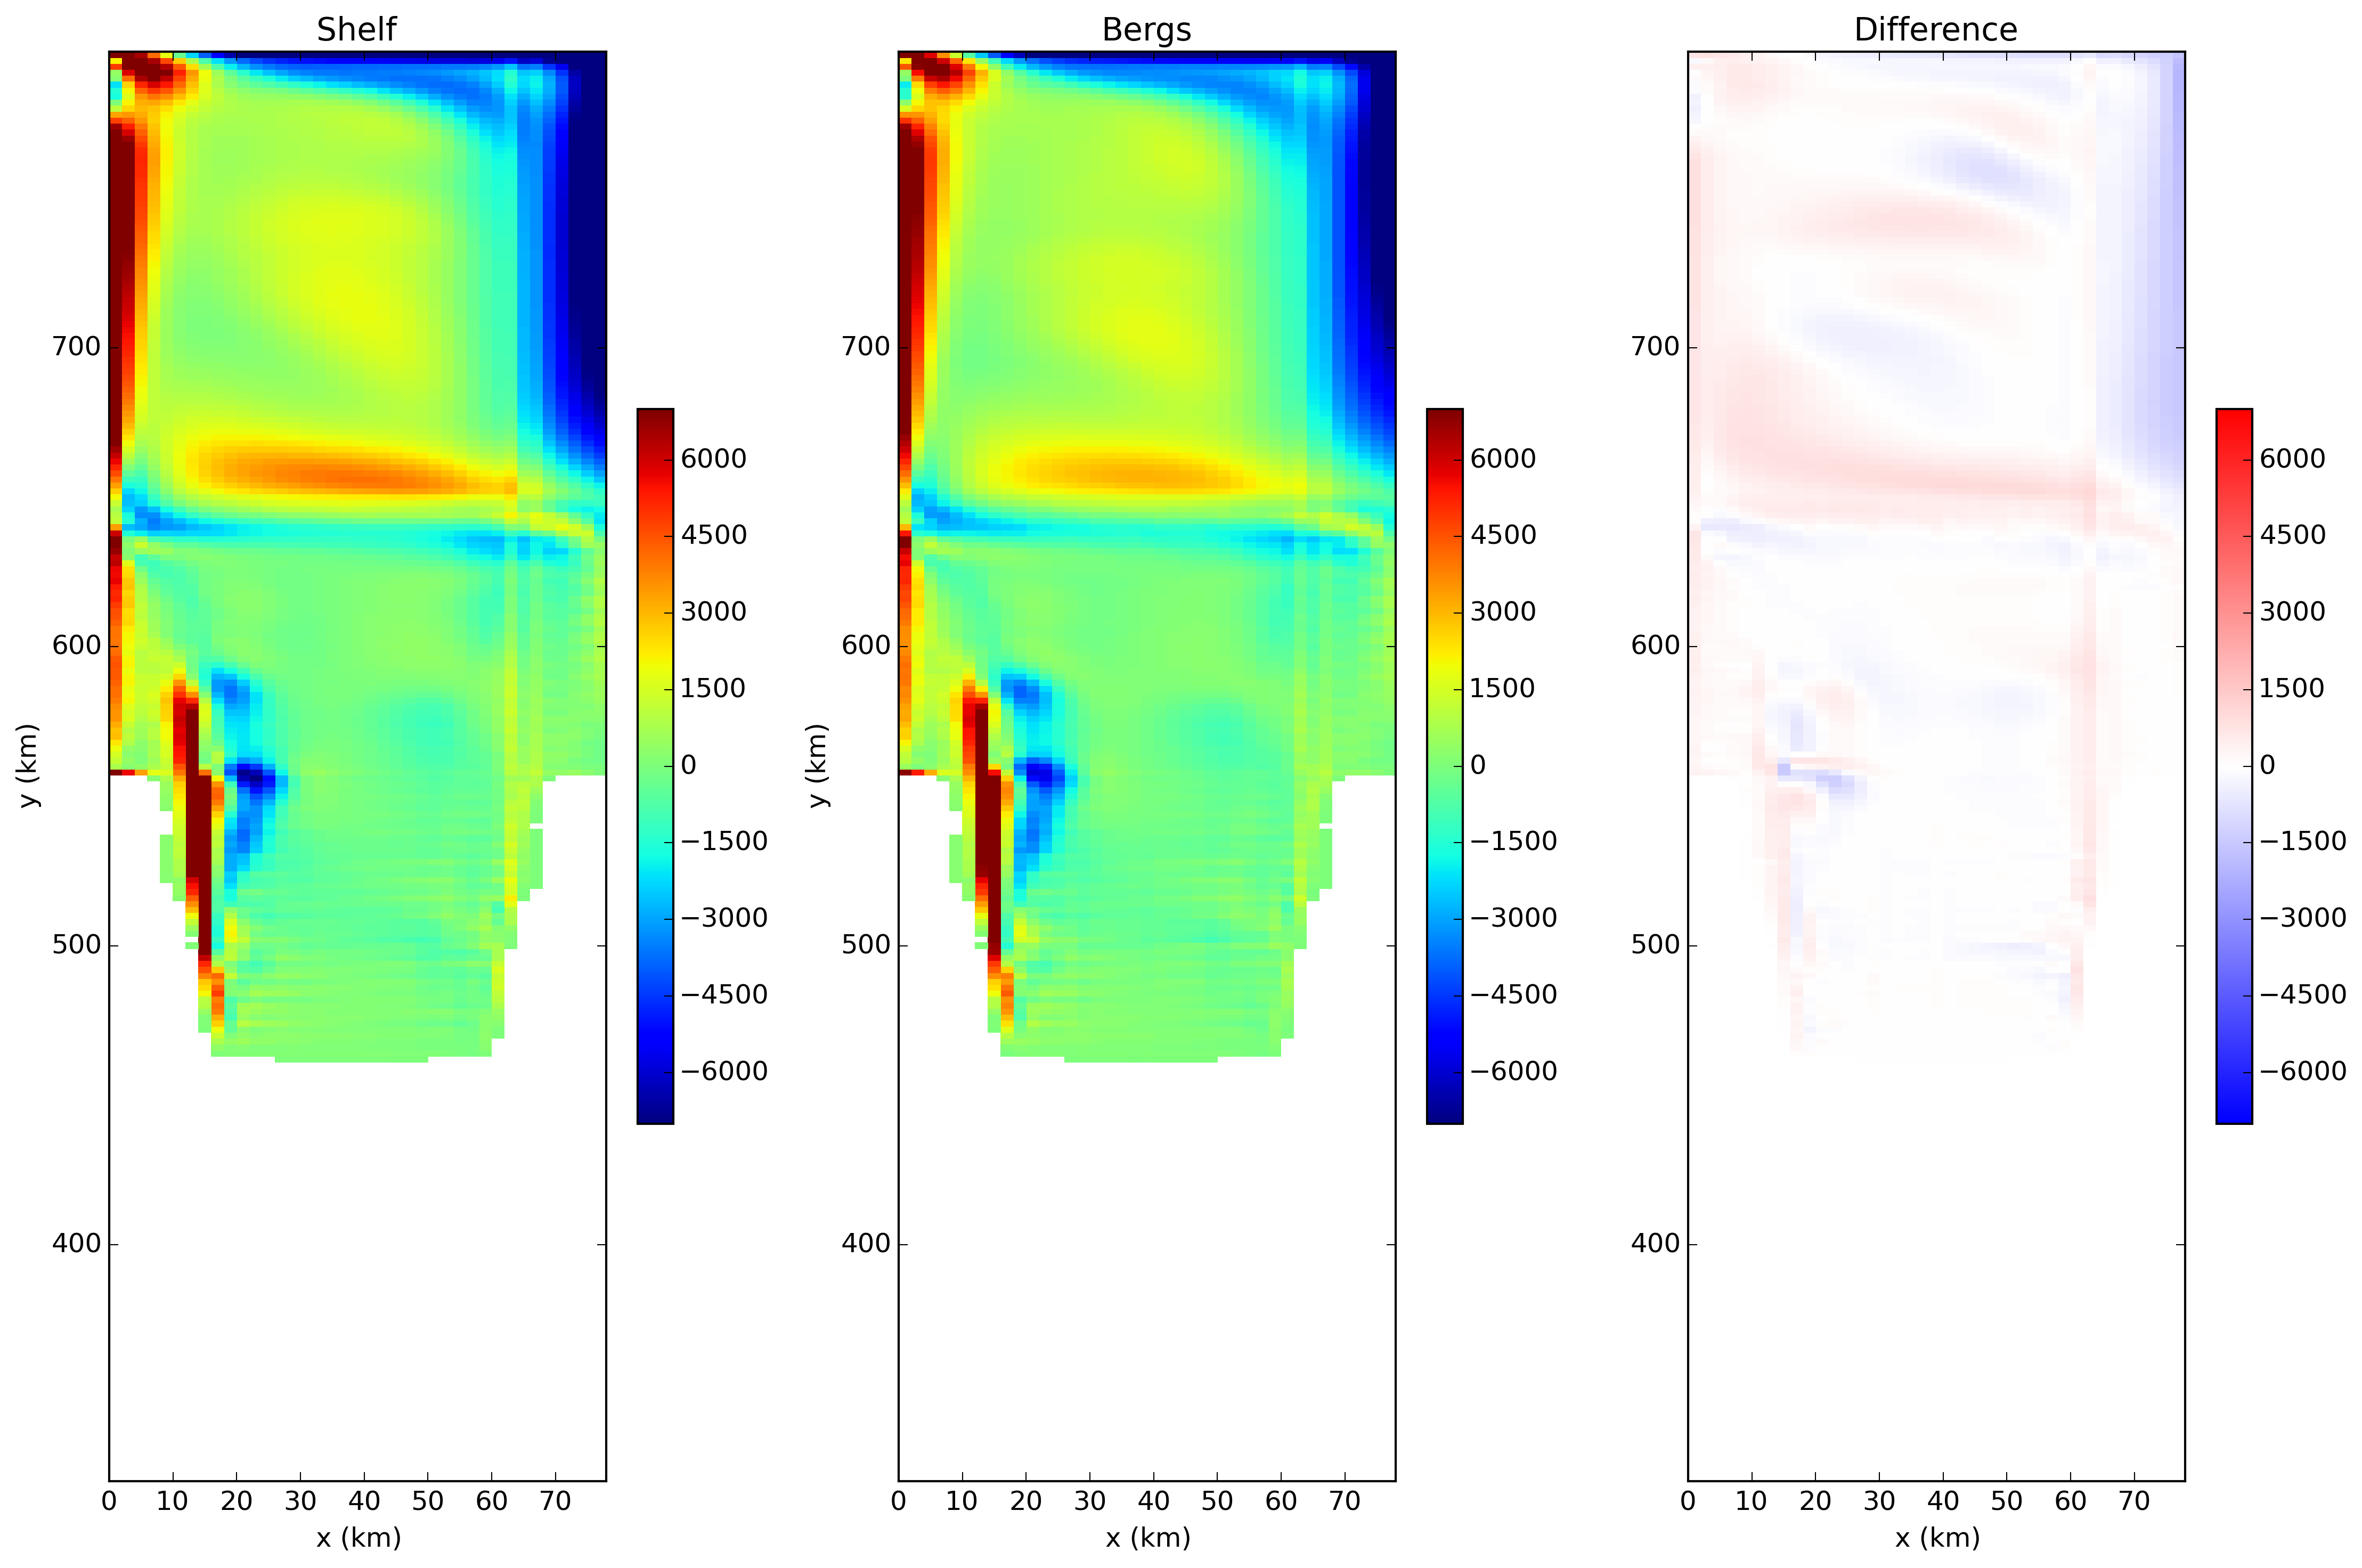
\includegraphics[width=0.99\textwidth]{Figures/ALE_z_static_shelf_comparison_barotropic_sf.png}
\includegraphics[width=0.99\textwidth]{Diagrams/Iceberg_scehmatic_with_red.pdf}
\caption{ {{\small Schematic illustrating how the ocean hydrography is affected by iceberg calving. Cool and warm water anomalies are indicated in blue and red, respectively, and ocean currents are shown using arrows.

Stage 1, iceberg detachment (a, b): as the iceberg detaches, water column stretching behind the iceberg causes warm water anomalies behind the iceberg. The conservation of PV caused by this stretching gives rise to a pair zonal jets behind and below the iceberg. Similarly, the contracting water column in front of the iceberg creates cool anomalies, and drives a zonal jet in front and below the iceberg.

Stage 2, iceberg rotation (c, d): as the iceberg drifts away from the ice shelf, it rotates causing the jets around it to change direction. The newly orientated jet in front of the iceberg drives water towards to ice shelf, which subducts at the ice front, causing subsurface cooling.

Stage 3, cooling below the ice shelf (e, f): as the iceberg moves away from the ice shelf, it interacts with the boundary currents, which are diverted by the presence of the iceberg. At the ice front, the cool water anomalies are advected into the ice-shelf cavity, eventually leading to reduced melt rates throughout the cavity.

The warm water surface anomalies behind the iceberg after calving (panel a), move with the iceberg as it drifts (panel b), and entirely surround the iceberg as it continues to drift into the open ocean (panel c).

}


}}
\end{center}
%FIgure created by \end{center}
\label{fig:Schematic_of_calving}
\end{figure}
 \clearpage



\begin{figure}
\begin{center}
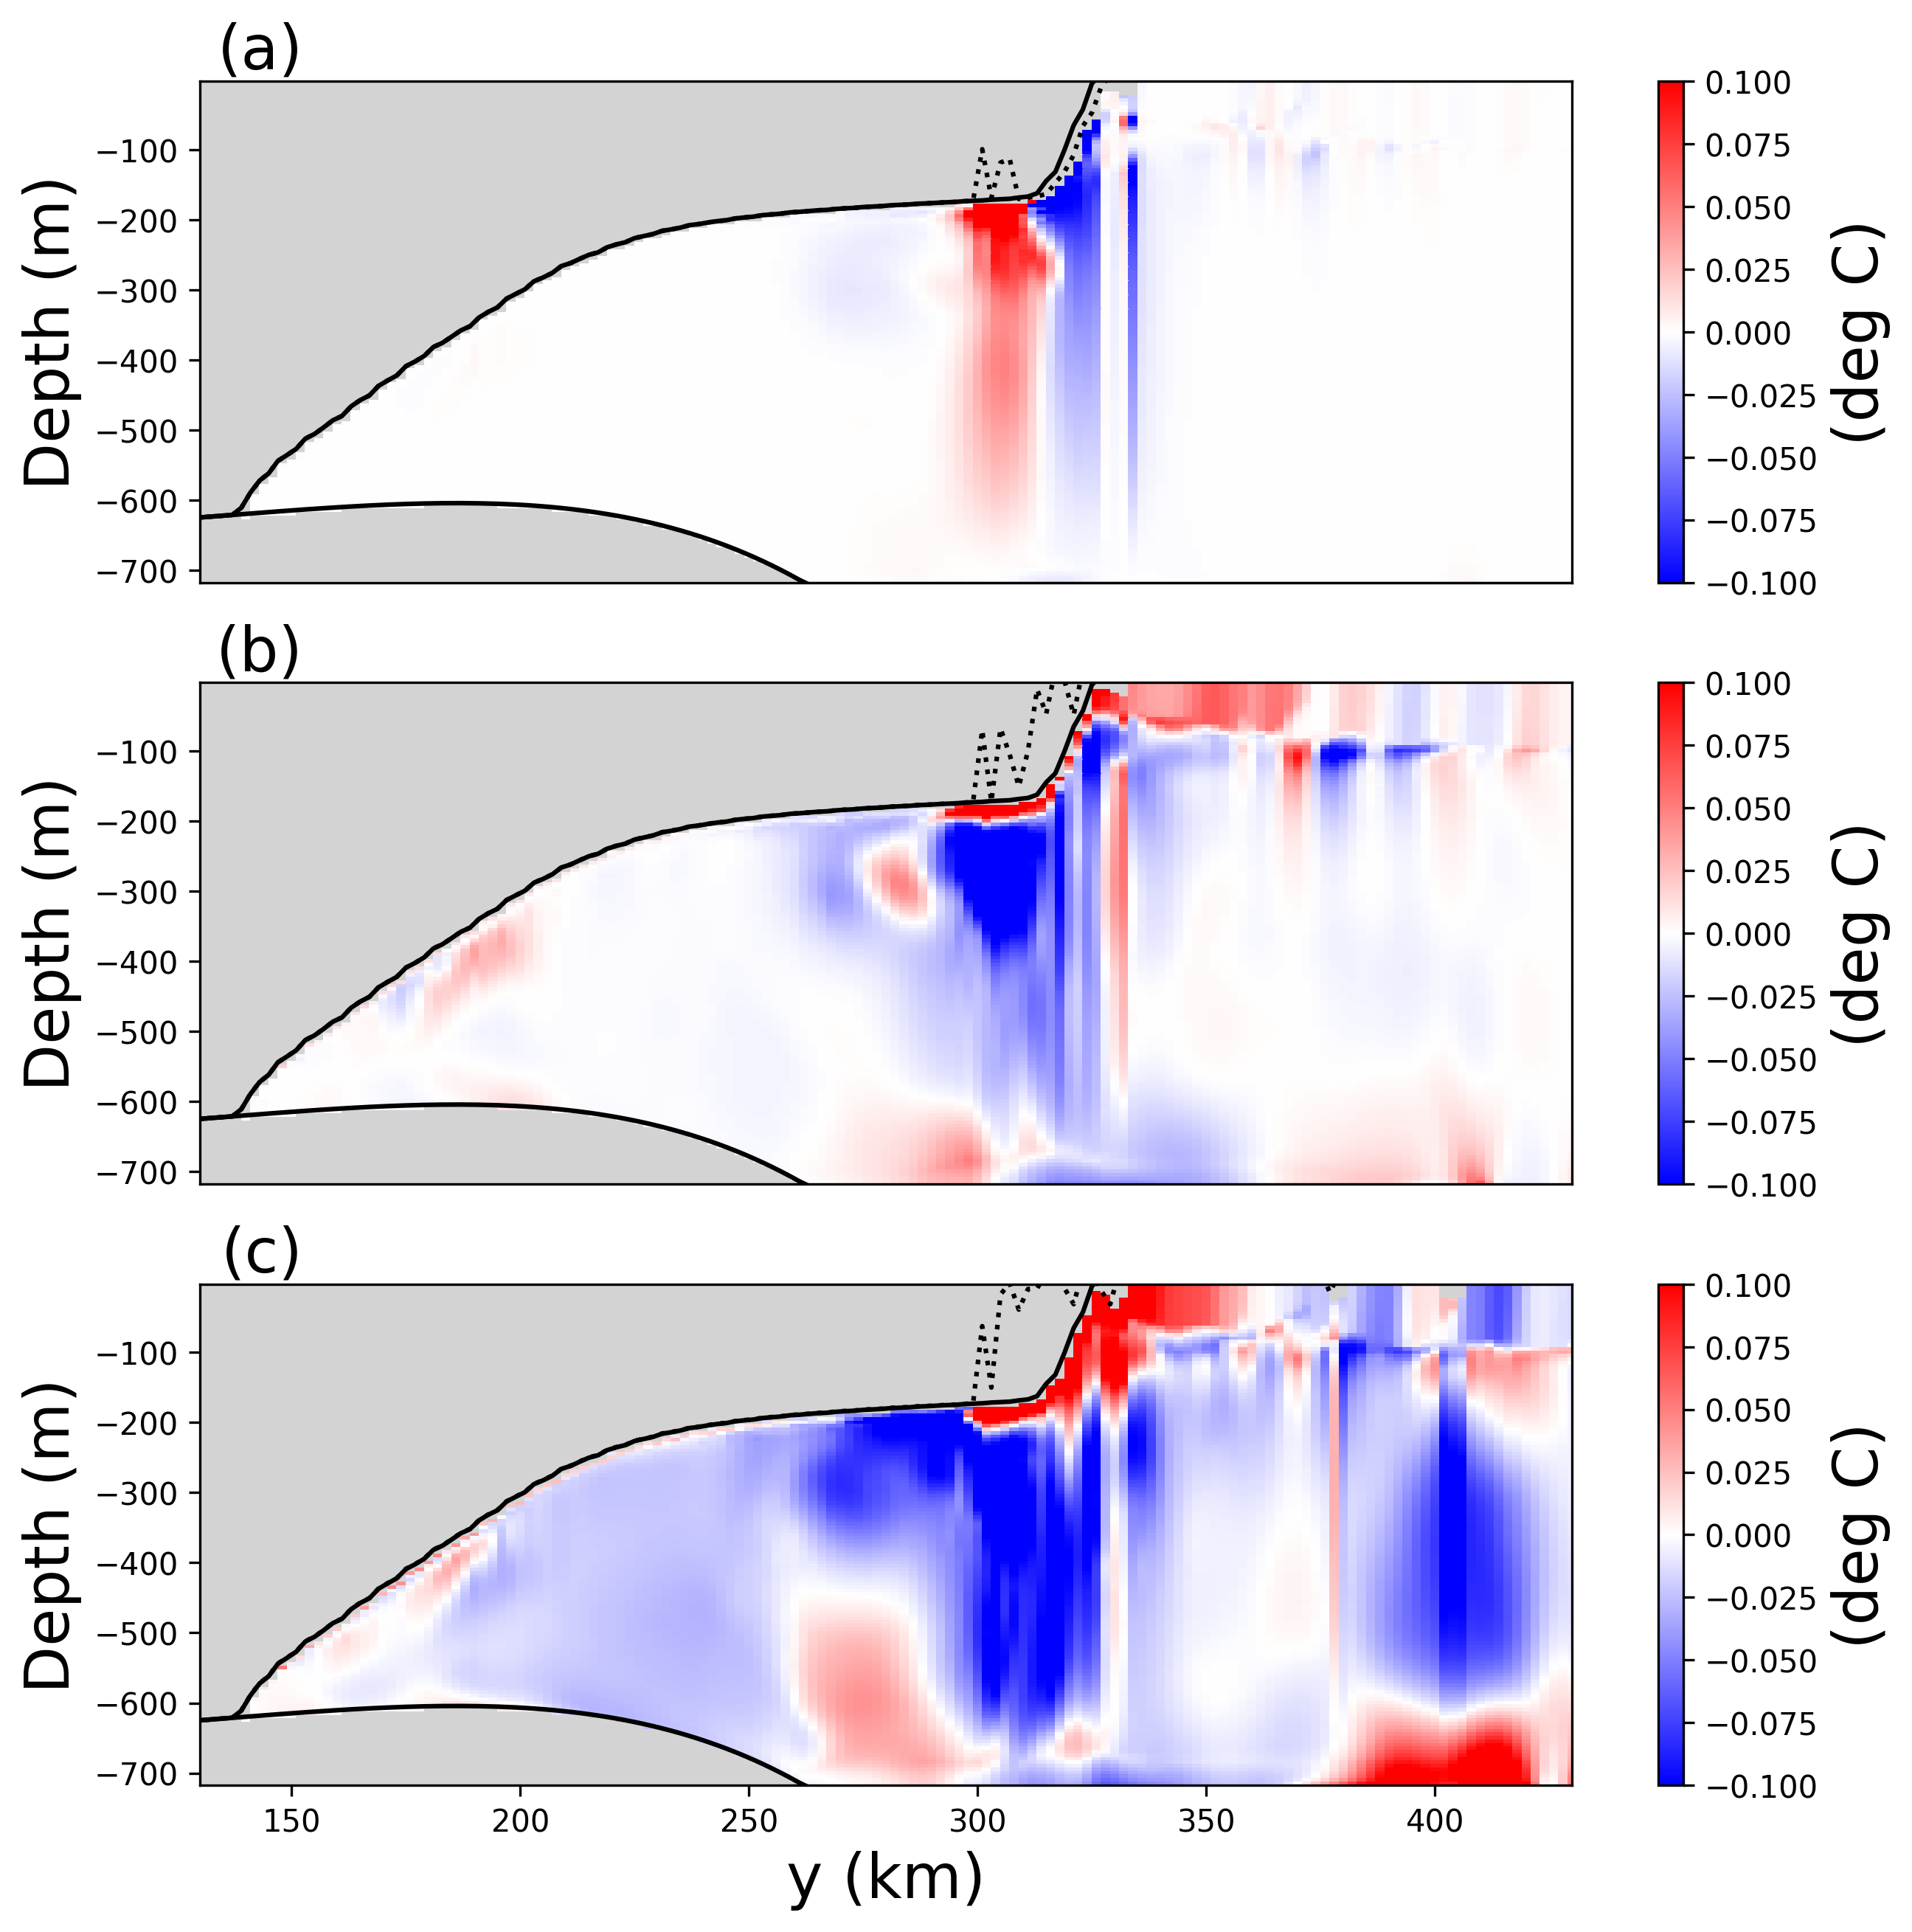
\includegraphics[width=0.99\textwidth]{Figures/snapshots_Wind_Wind_Collapse_temp_zold_x20_anomaly.png}
\caption{ {Snapshots of vertical sections of ocean temperature anomaly at $x$=40~km in the iceberg-calving experiment. The anomalies are relative to pre-calving temperatures. Snapshots are taken (a) 1, (b) 15, and (c) 50 days after calving. In each panel, the base of the ice before calving and at the time of the snapshot are shown by the solid and dashed black lines, respectively. Positions that were not the ocean interior at in both snapshots are masked in grey. The position of the vertical transects is shown by the black dashed lines in Figure \ref{fig:SST_snapshots}a.}}
\end{center}
%FIgure created by \end{center}
\label{fig:Temperature_section_Collapse_yz}
\end{figure}
 \clearpage



\begin{figure}
\begin{center}
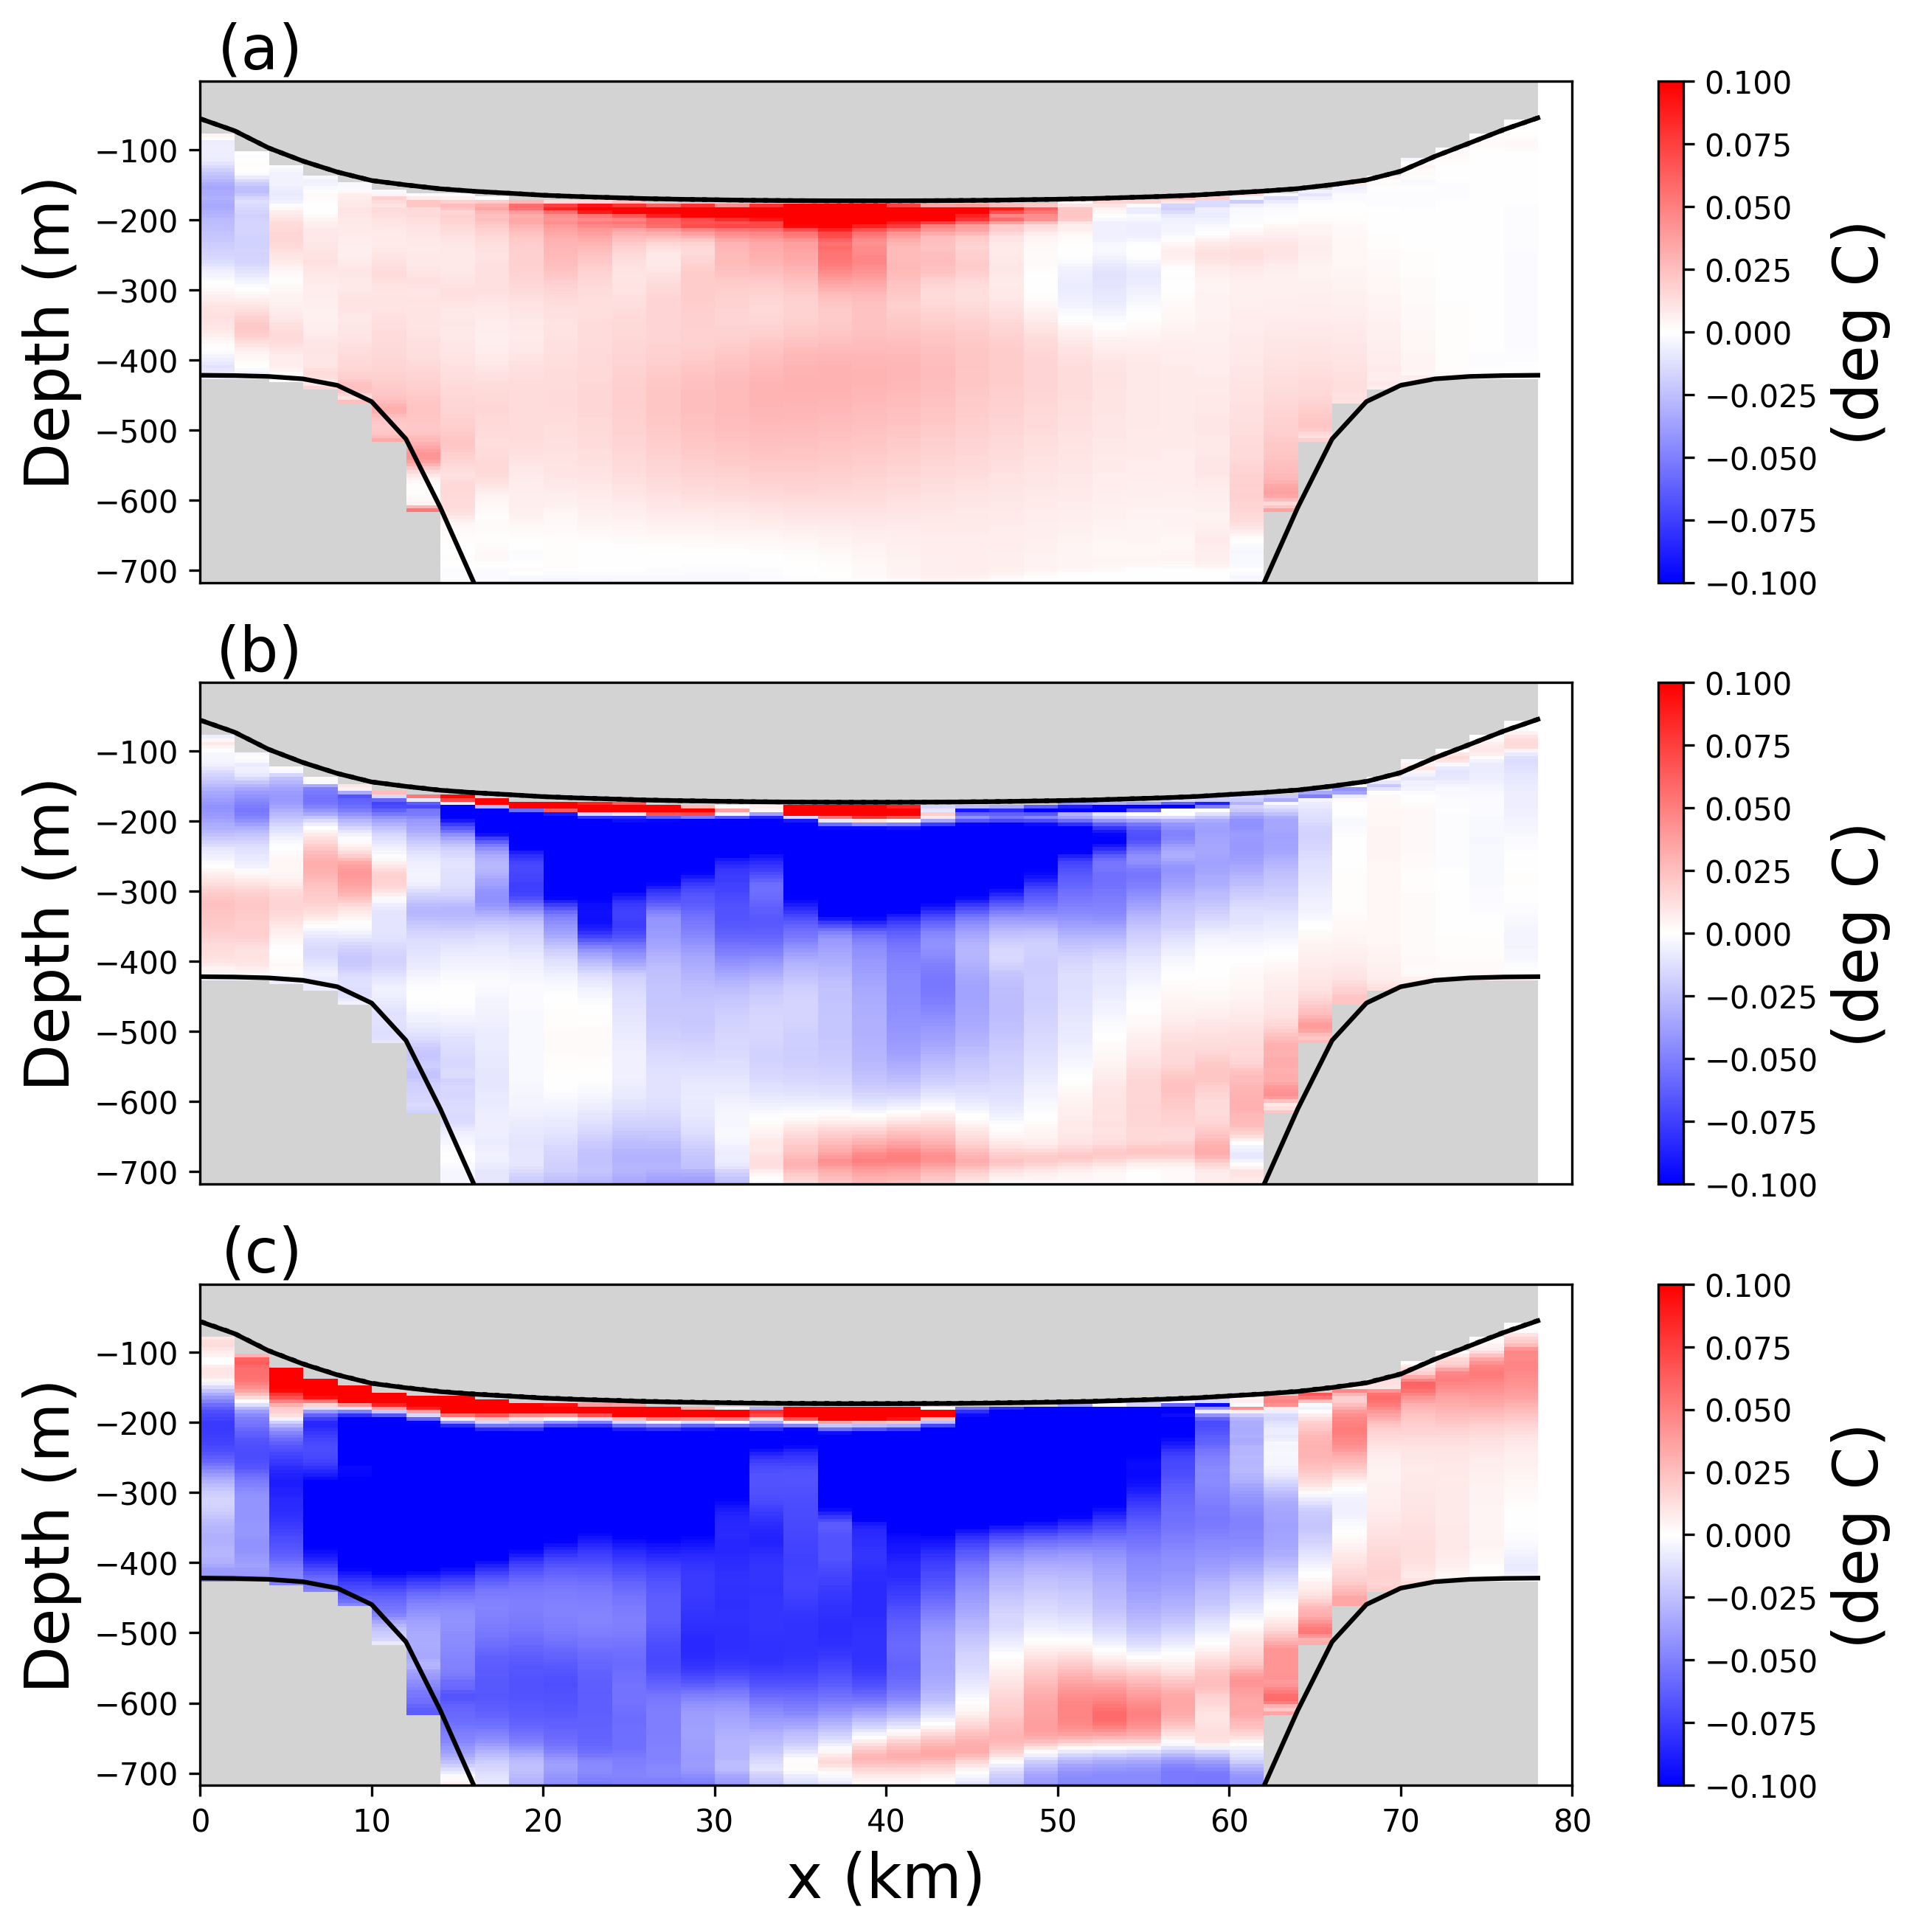
\includegraphics[width=0.99\textwidth]{Figures/snapshots_Wind_Wind_Collapse_temp_zold_x149_anomaly_mask.png}
%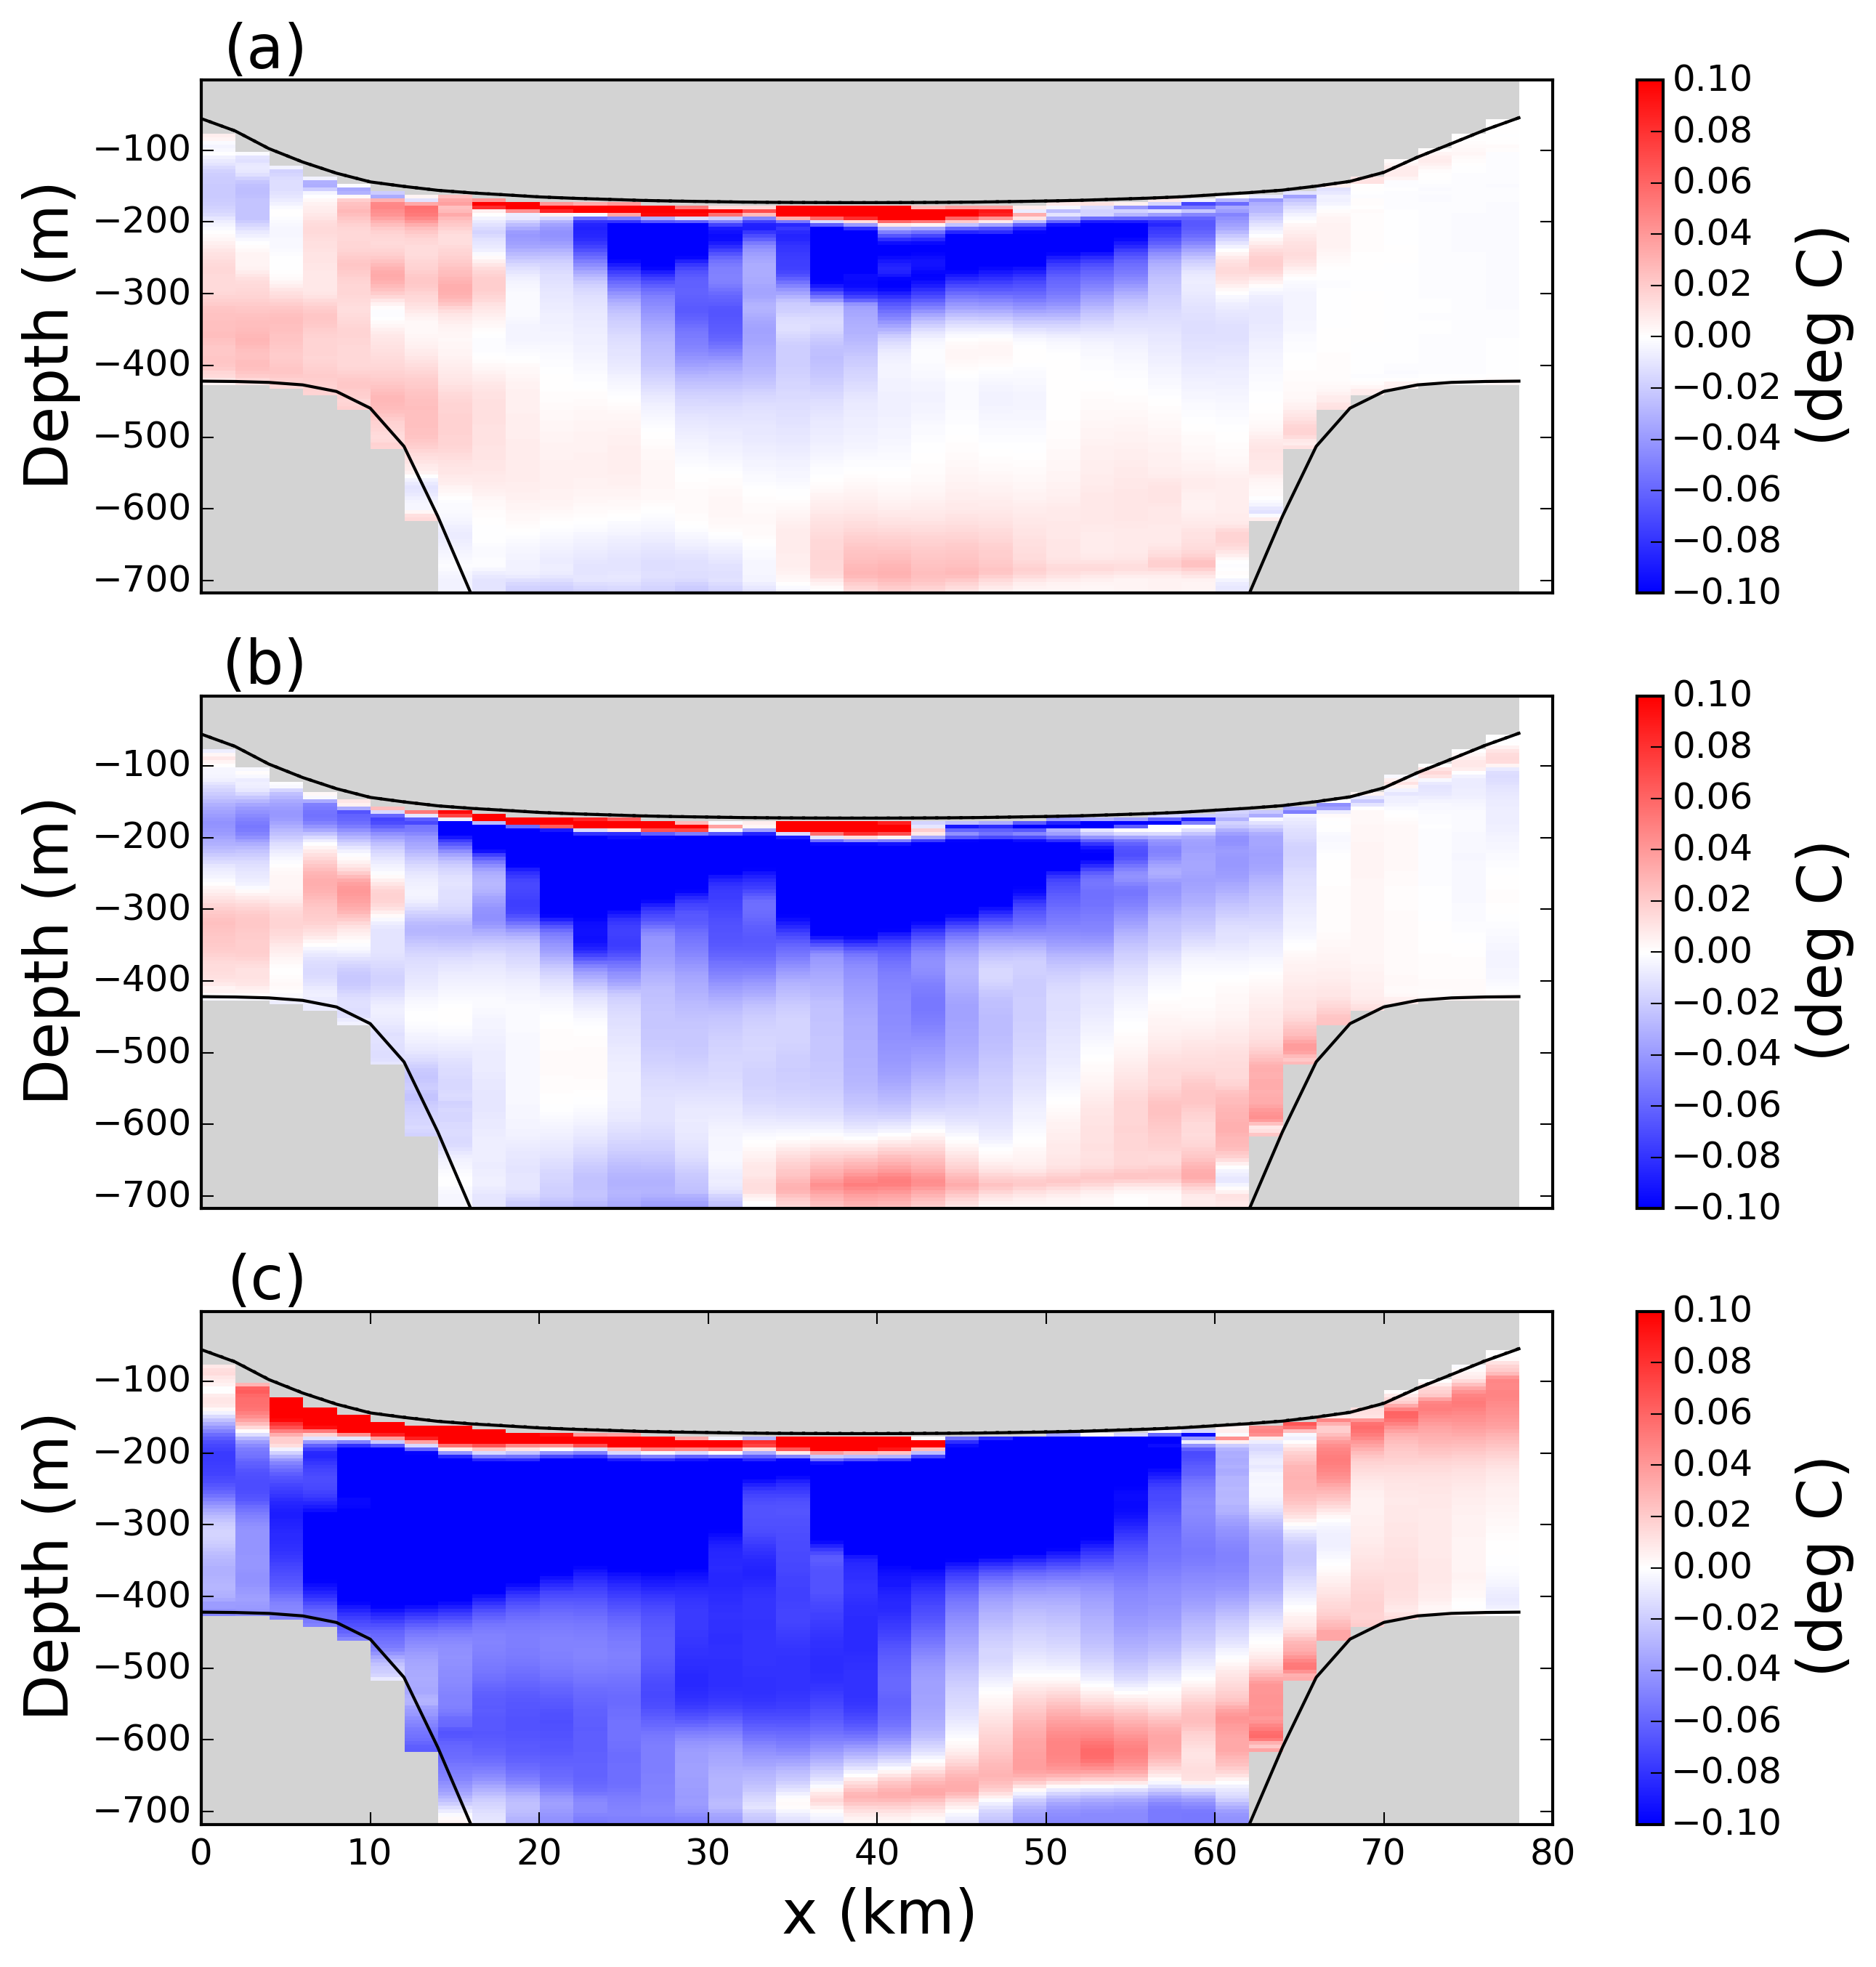
\includegraphics[width=0.99\textwidth]{Figures/snapshots_Wind_Wind_Collapse_temp_zold_x149_anomaly.png}
\caption{ {Snapshots of vertical sections of ocean temperature anomaly at $y$=300~km in the tabular-iceberg-calving experiment. The anomalies are relative to pre-calving temperatures. Snapshots are taken (a) 1, (b) 15, and (c) 50 days after calving. The position of the vertical transects is shown by the blue dashed lines in Figure \ref{fig:SST_snapshots}a. }}
\end{center}
%FIgure created by \end{center}
\label{fig:Temperature_section_Collapse_xz}
\end{figure}
 \clearpage
 
 

 
\begin{figure}
\begin{center}
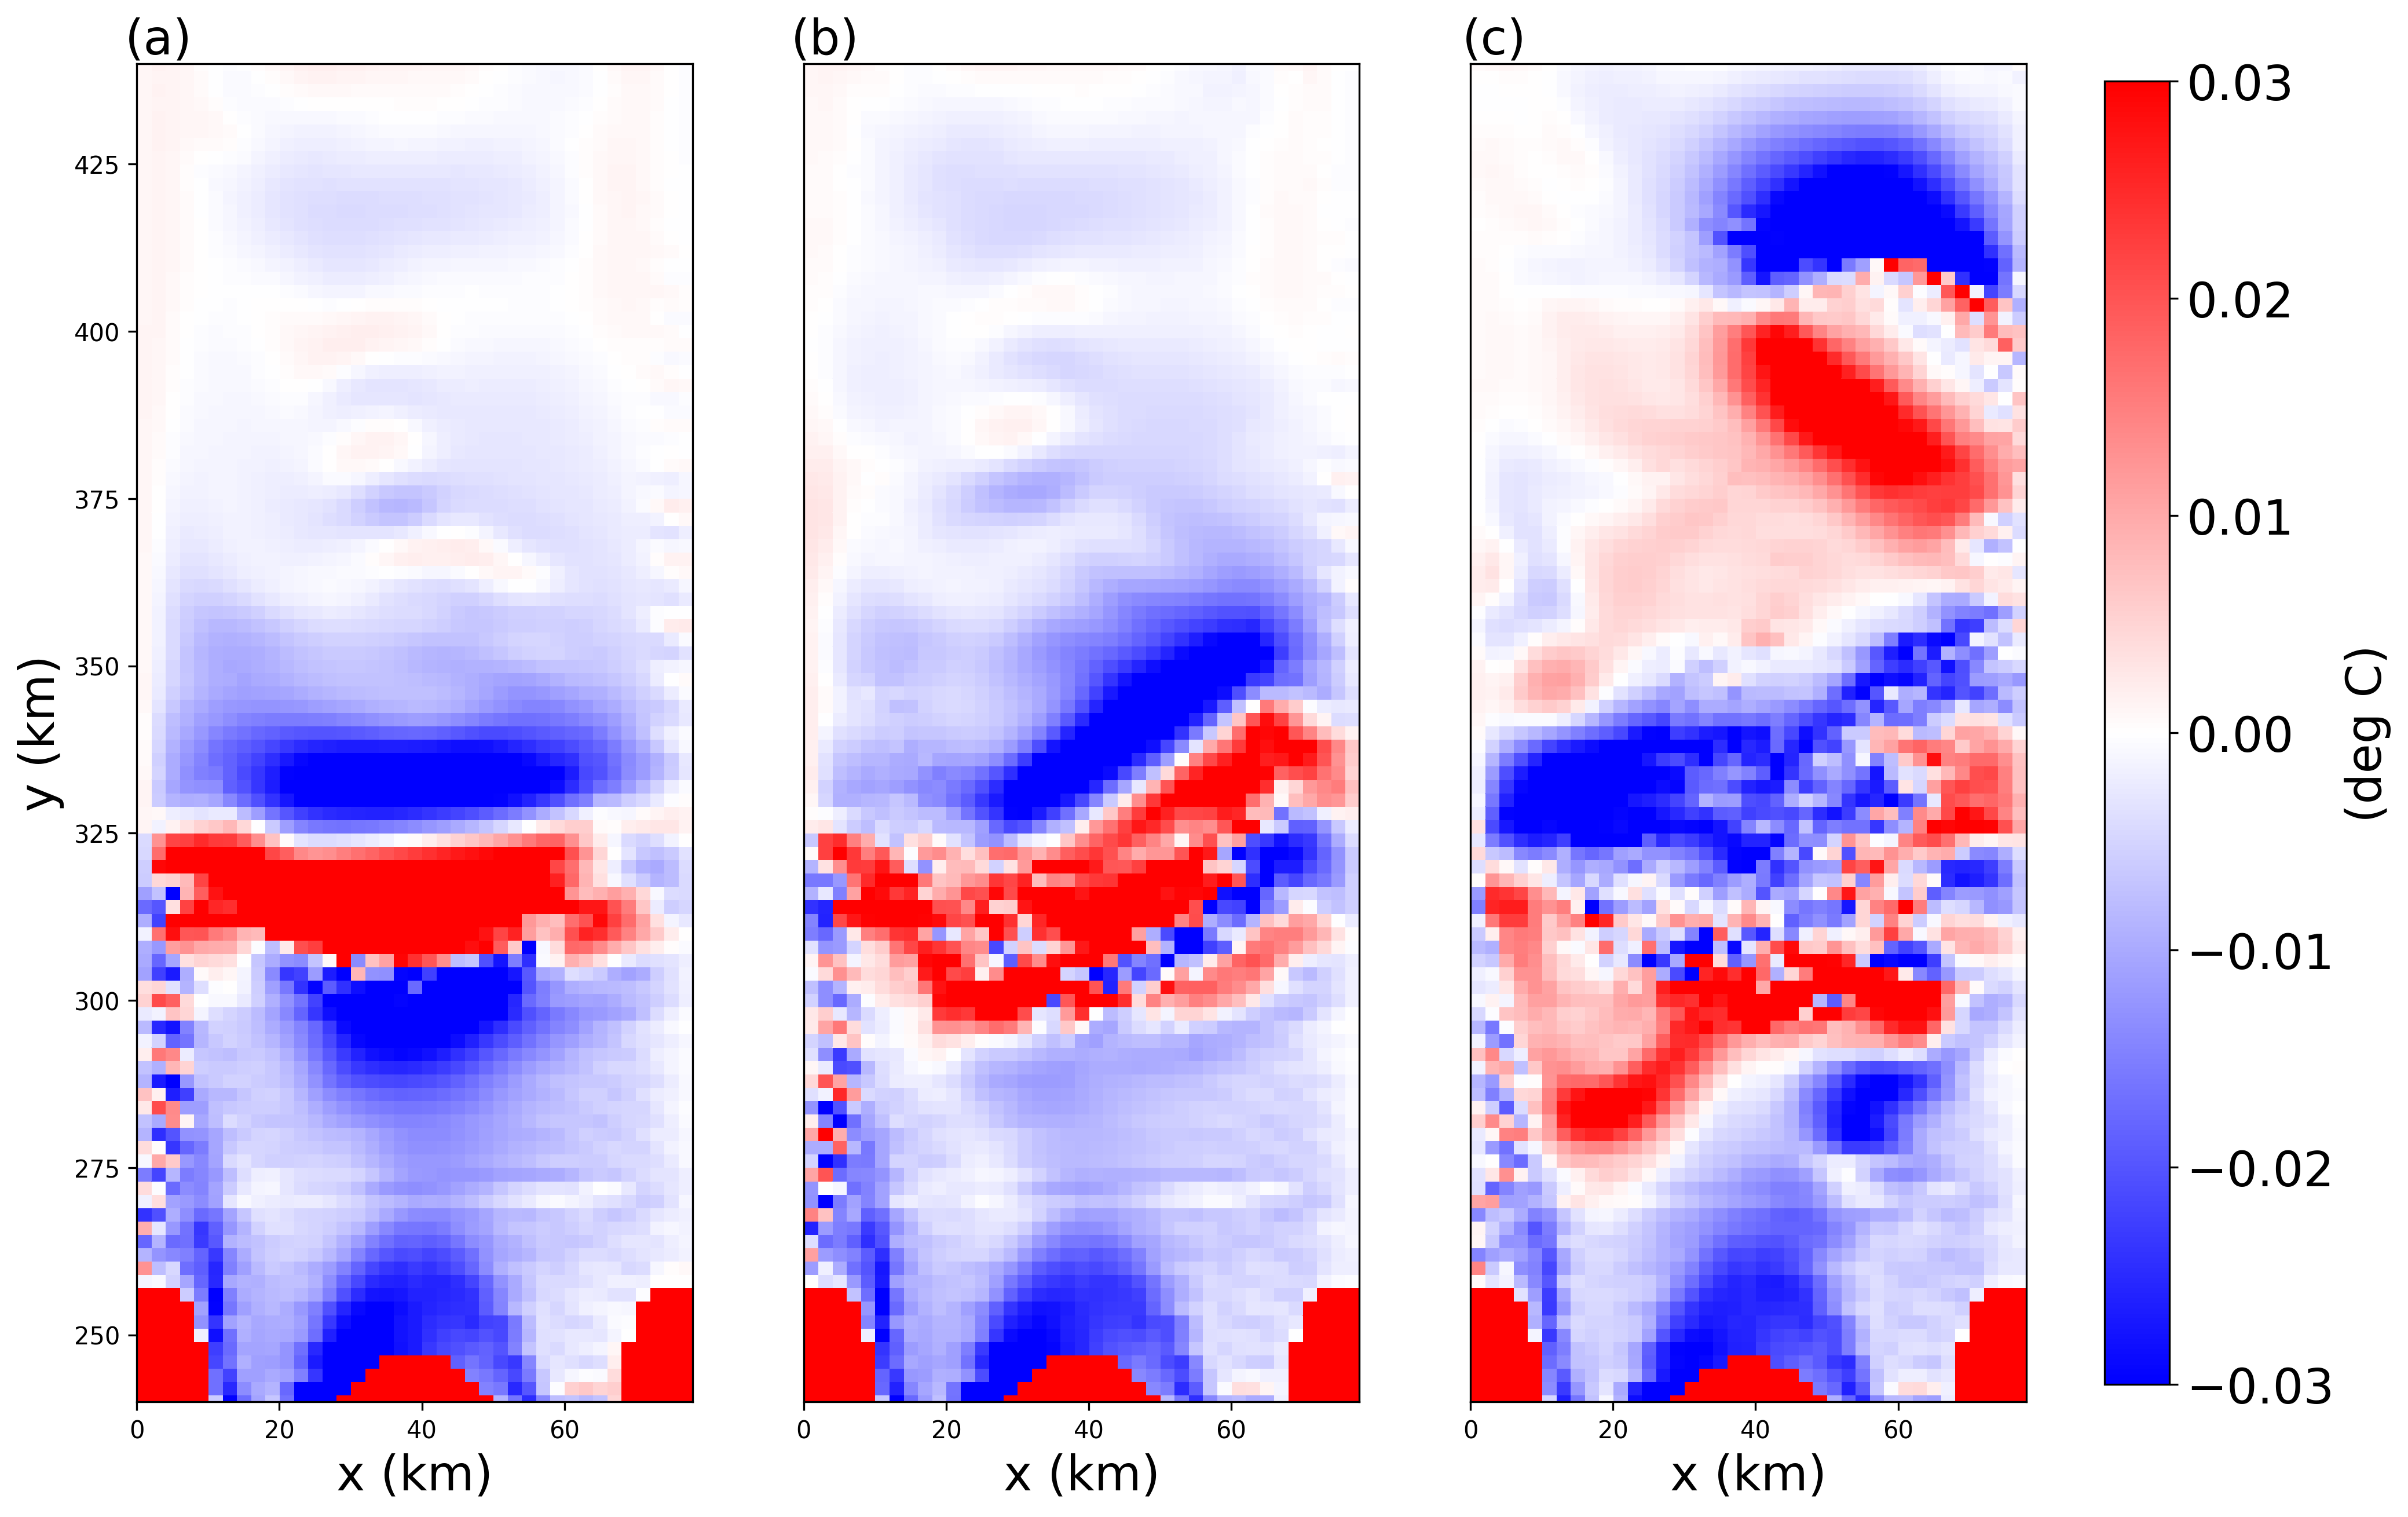
\includegraphics[width=0.99\textwidth]{Figures/snapshots_Wind_Wind_Collapse_u.png}
\caption{ {Snapshots of ocean zonal velocity at $z$=197.5~m(?) in the iceberg-calving experiment. Snapshots are taken (a) 1, (b) 15, and (c) 50 days after calving. \textcolor{red}{I should include an outline of the iceberg shape in this figure}}}
\end{center}
%FIgure created by \end{center}
\label{fig:u_velocity_horizontal}
\end{figure}
 \clearpage

 
\begin{figure}
\begin{center}
%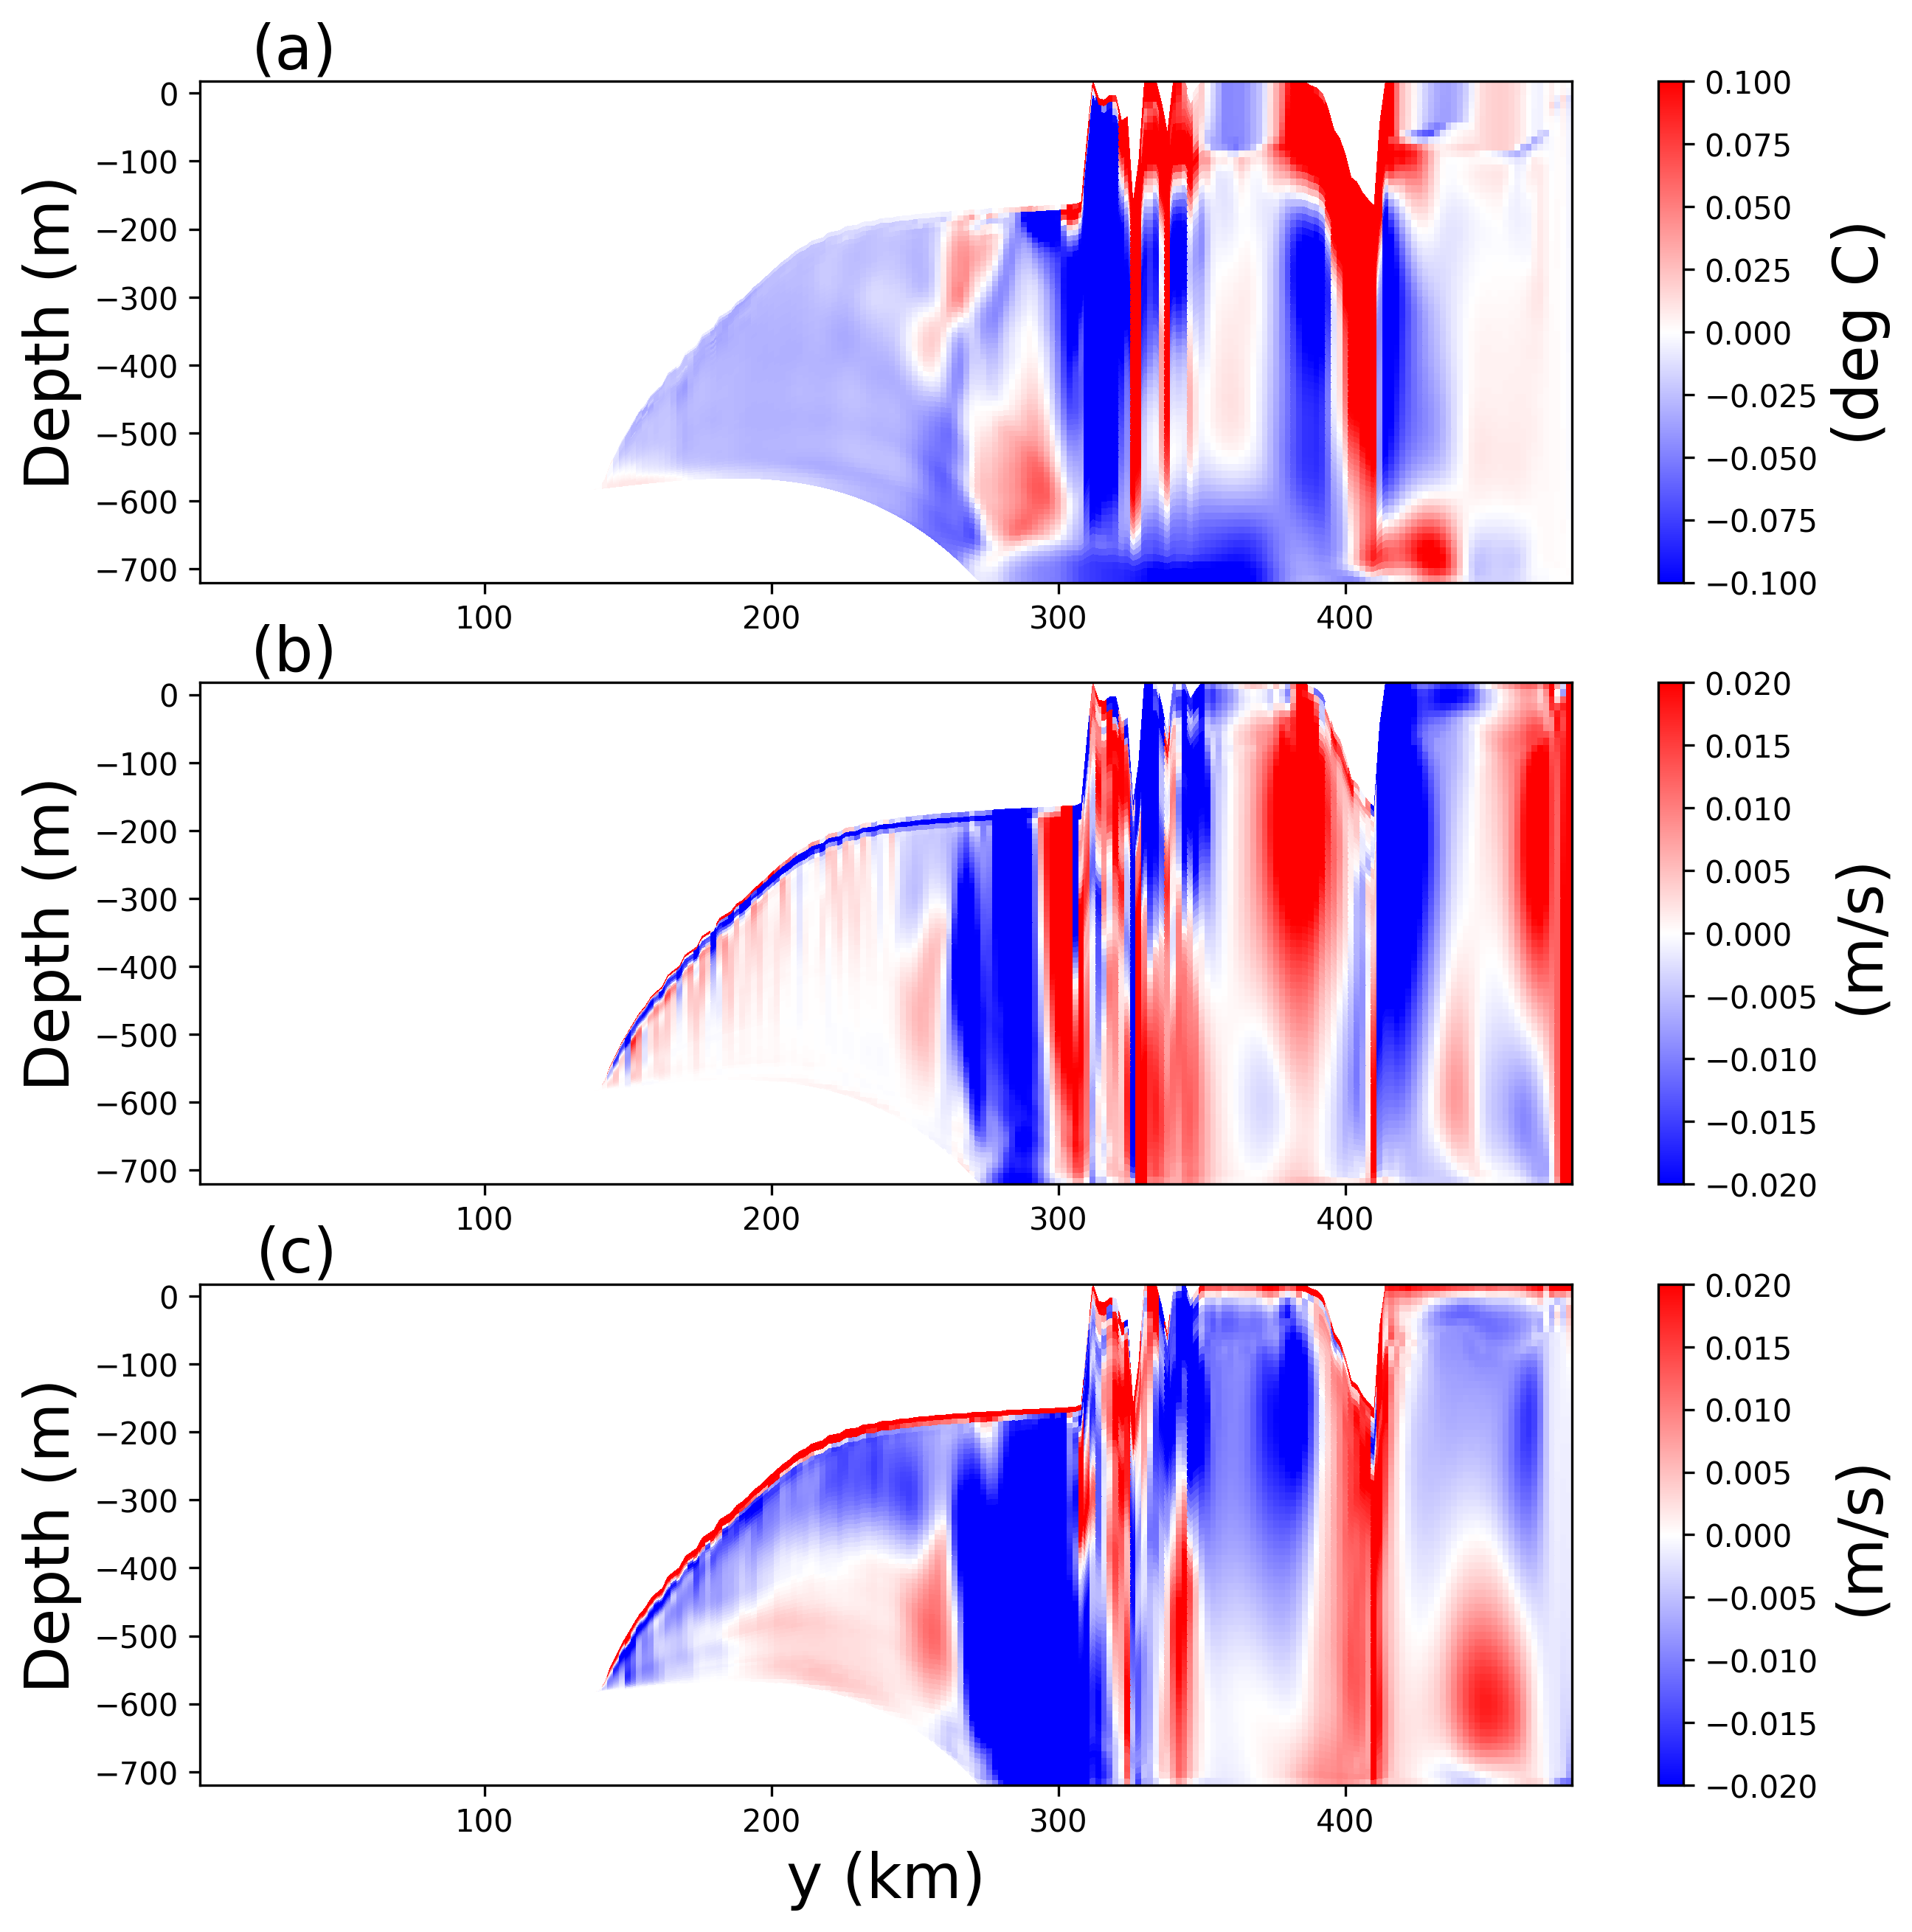
\includegraphics[width=0.99\textwidth]{Figures/Wind_static_shelf_solo_temp_u_v_calved.png}
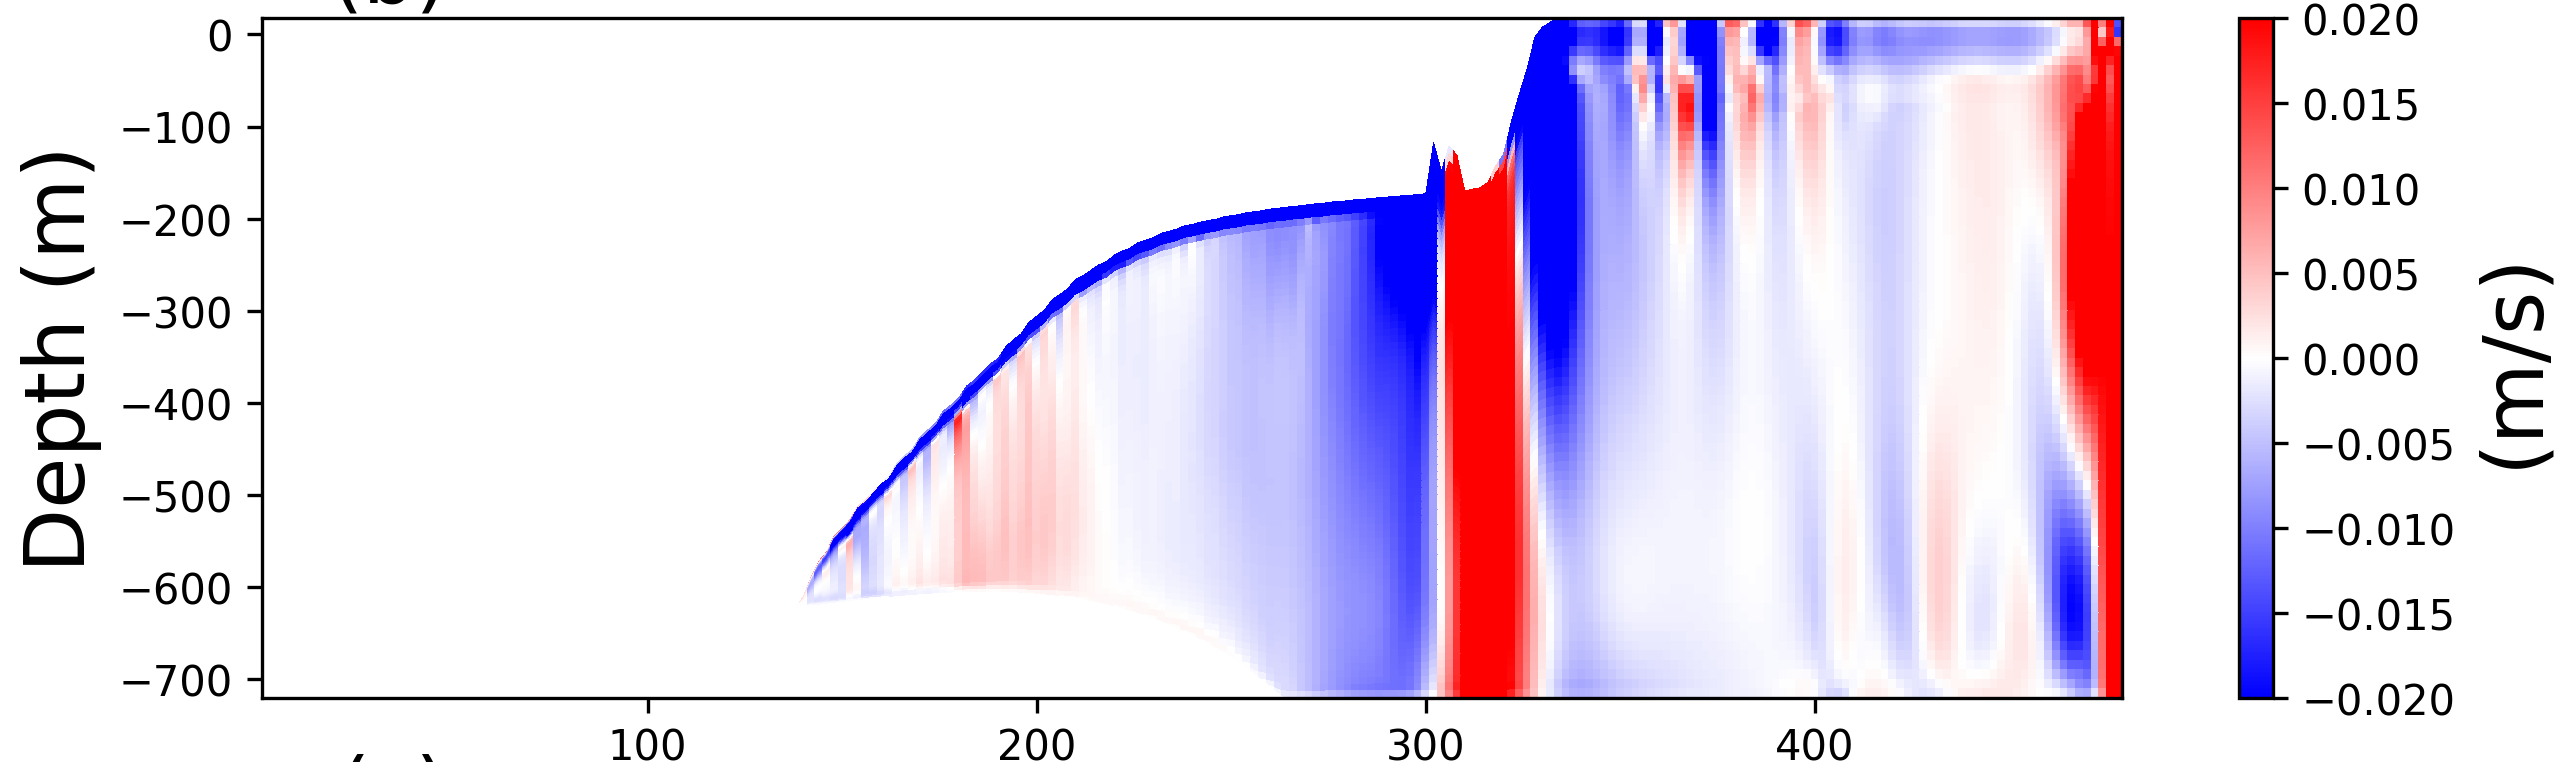
\includegraphics[width=0.99\textwidth]{Figures/Wind_static_shelf_solo_u_cropped.png}

\caption{ {Snapshot of vertical section of zonal velocity at $x$=40~km in the iceberg-calving experiment 1 day after calving. The position of the vertical transects is shown by the black dashed line in Figure \ref{fig:SST_snapshots}a. An eastward jet is observed beneath the iceberg, and westward jets are observed to the north and south of the iceberg.}}
\end{center}
%FIgure created by \end{center}
\label{fig:v_velocity_vertical}
\end{figure}
 \clearpage


  
\begin{figure}
\begin{center}
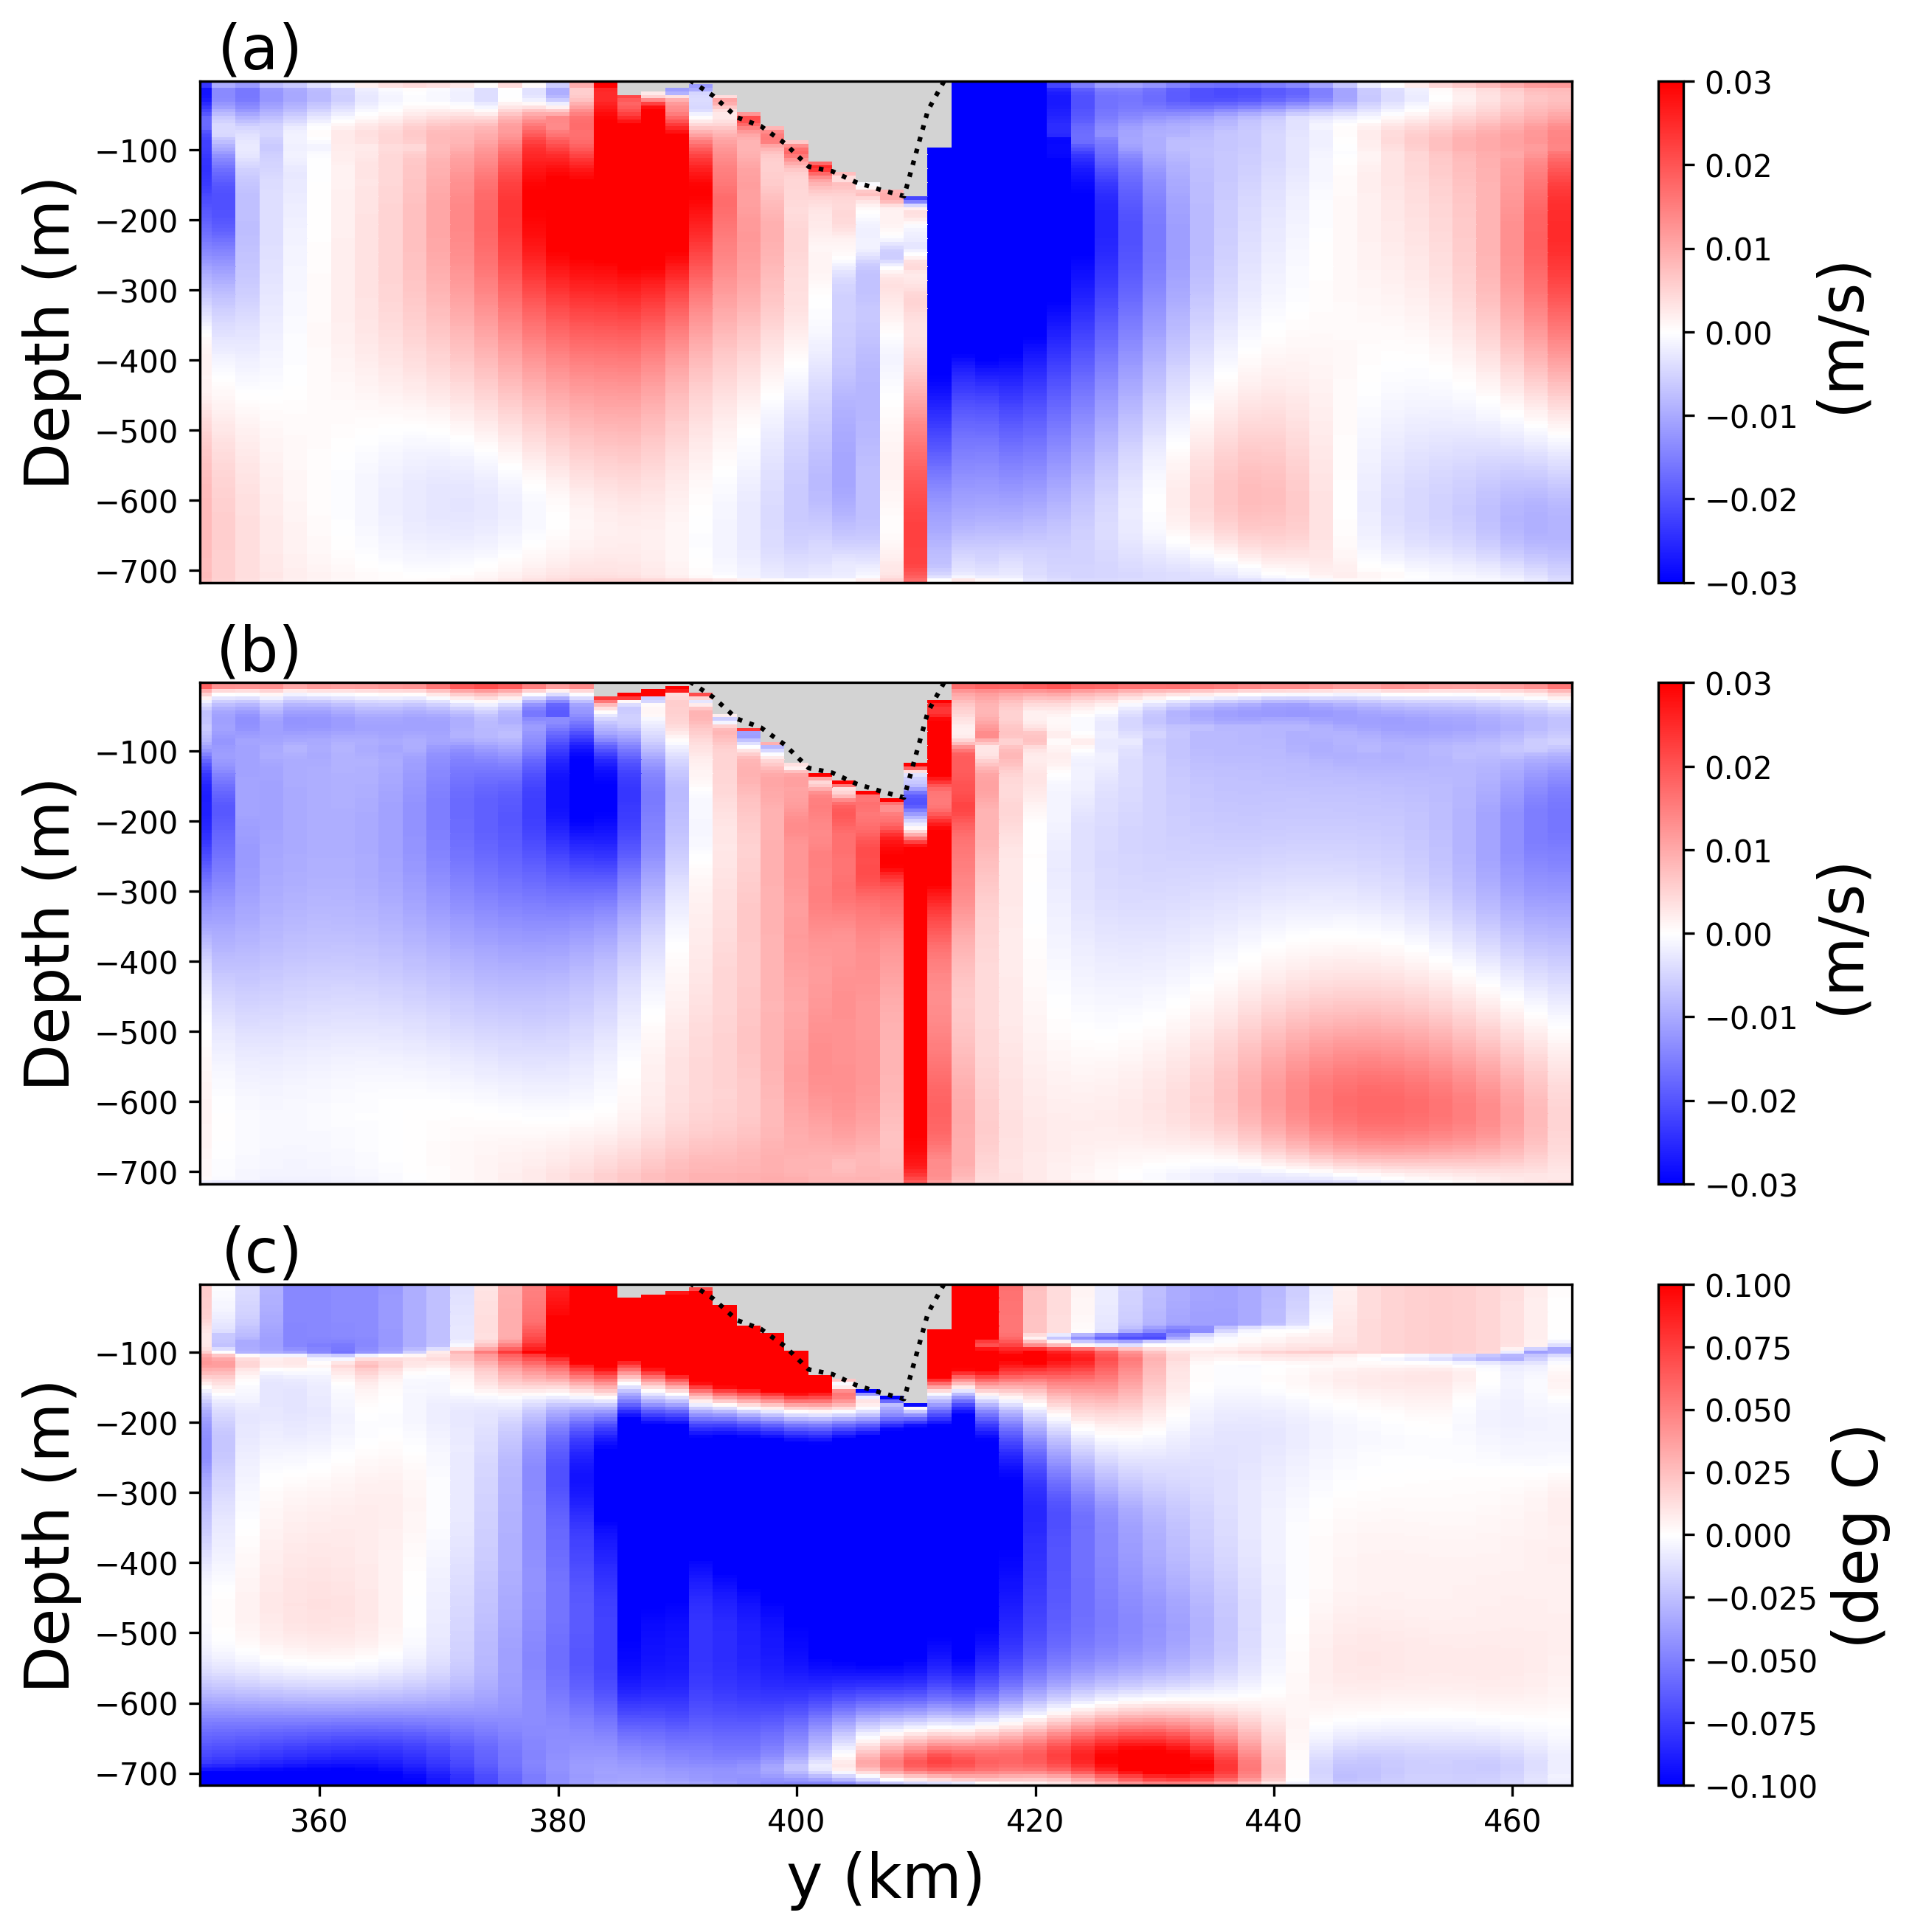
\includegraphics[width=0.99\textwidth]{Figures/snapshots_Wind_Wind_Collapse_temp_zold_x10_anomaly_mask.png}
\caption{ {Snapshots of vertical sections of ocean (a) zonal velocity, (b) meridional velocity,  and (c) temperature anomaly at $x$=60~km in the tabular-iceberg-calving experiment. The anomalies are relative to pre-calving temperatures. Snapshots are taken 50 days after calving. 
%The position of the vertical transects is shown by the dashed lines in Figure \ref{fig:SST_snapshots}c. 
\textcolor{red}{Should we add the position to Figure 2a?}}}
\end{center}
\label{fig:Taylor_column}
\end{figure}
 \clearpage
 
 


\begin{figure}
\begin{center}
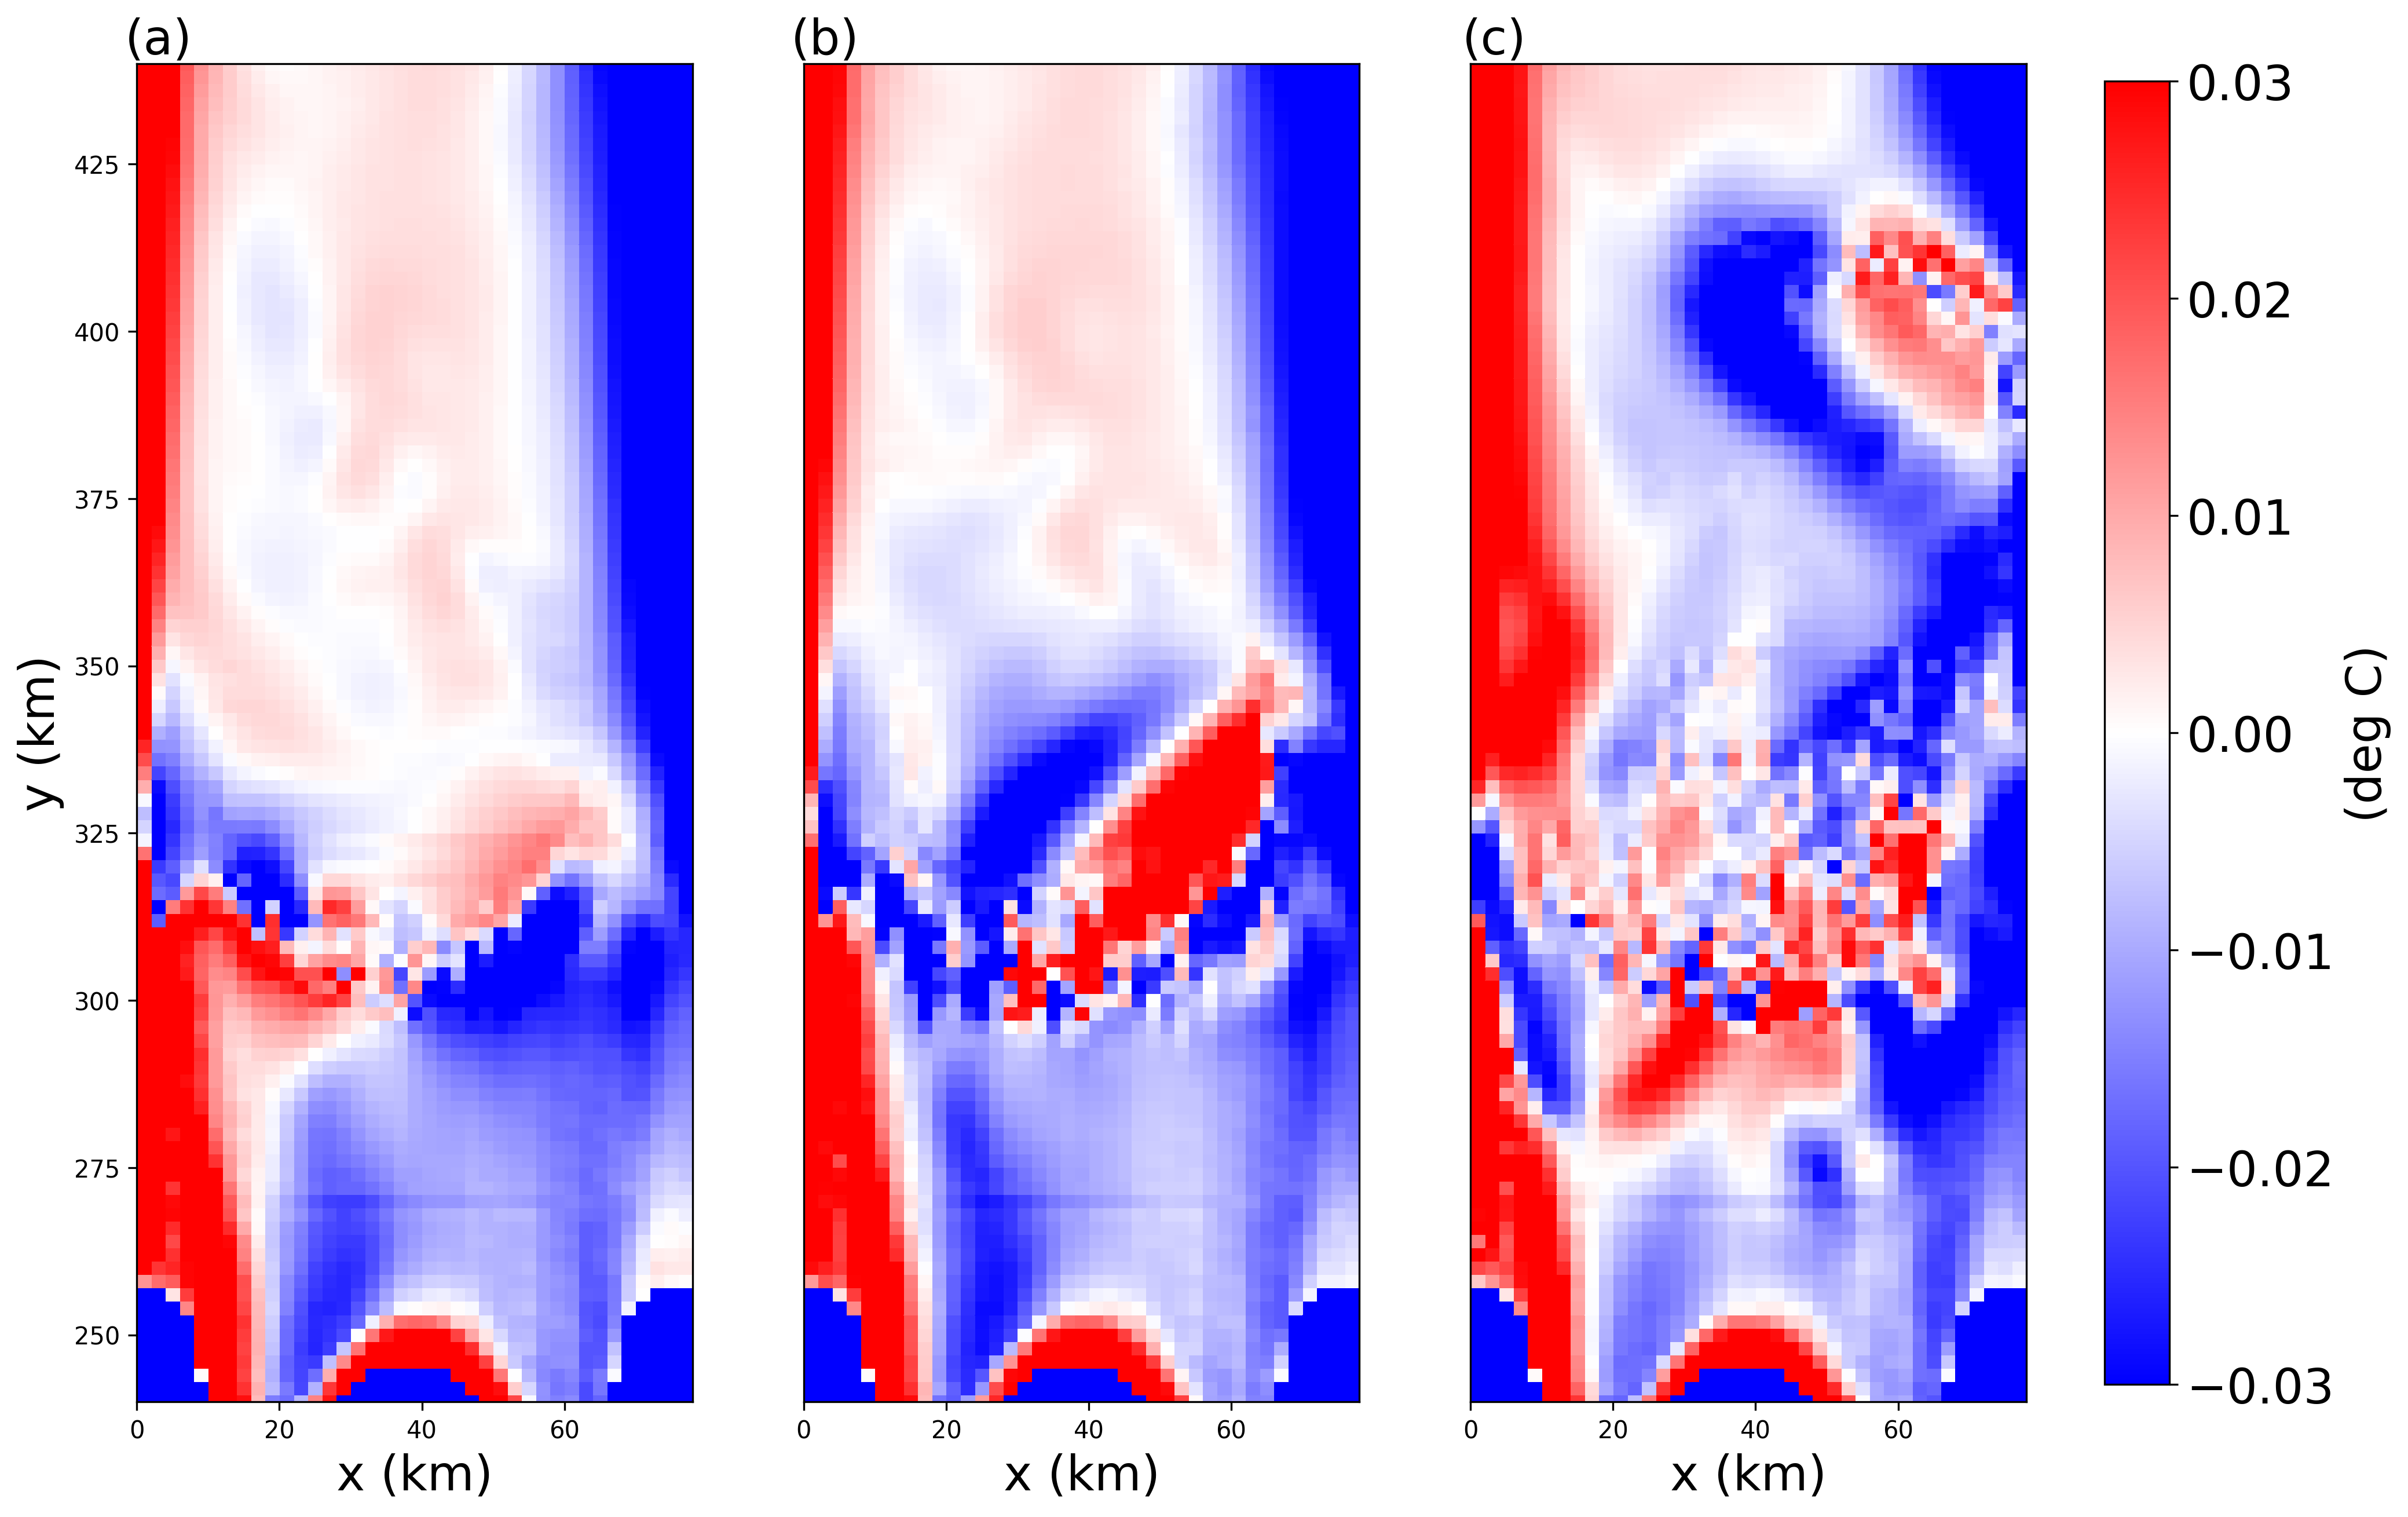
\includegraphics[width=0.99\textwidth]{Figures/snapshots_Wind_Wind_Collapse_v_z40_.png}
\caption{ {Snapshots of ocean meridional velocity at $z$=197.5~m in the iceberg-calving experiment. Snapshots are taken (a) 1, (b) 15, and (c) 50 days after calving. \textcolor{red}{I should include an outline of the iceberg shape in this figure}}}
\end{center}
%FIgure created by \end{center}
\label{fig:v_velocity_horizontal}
\end{figure}
 \clearpage





\begin{figure}
\begin{center}
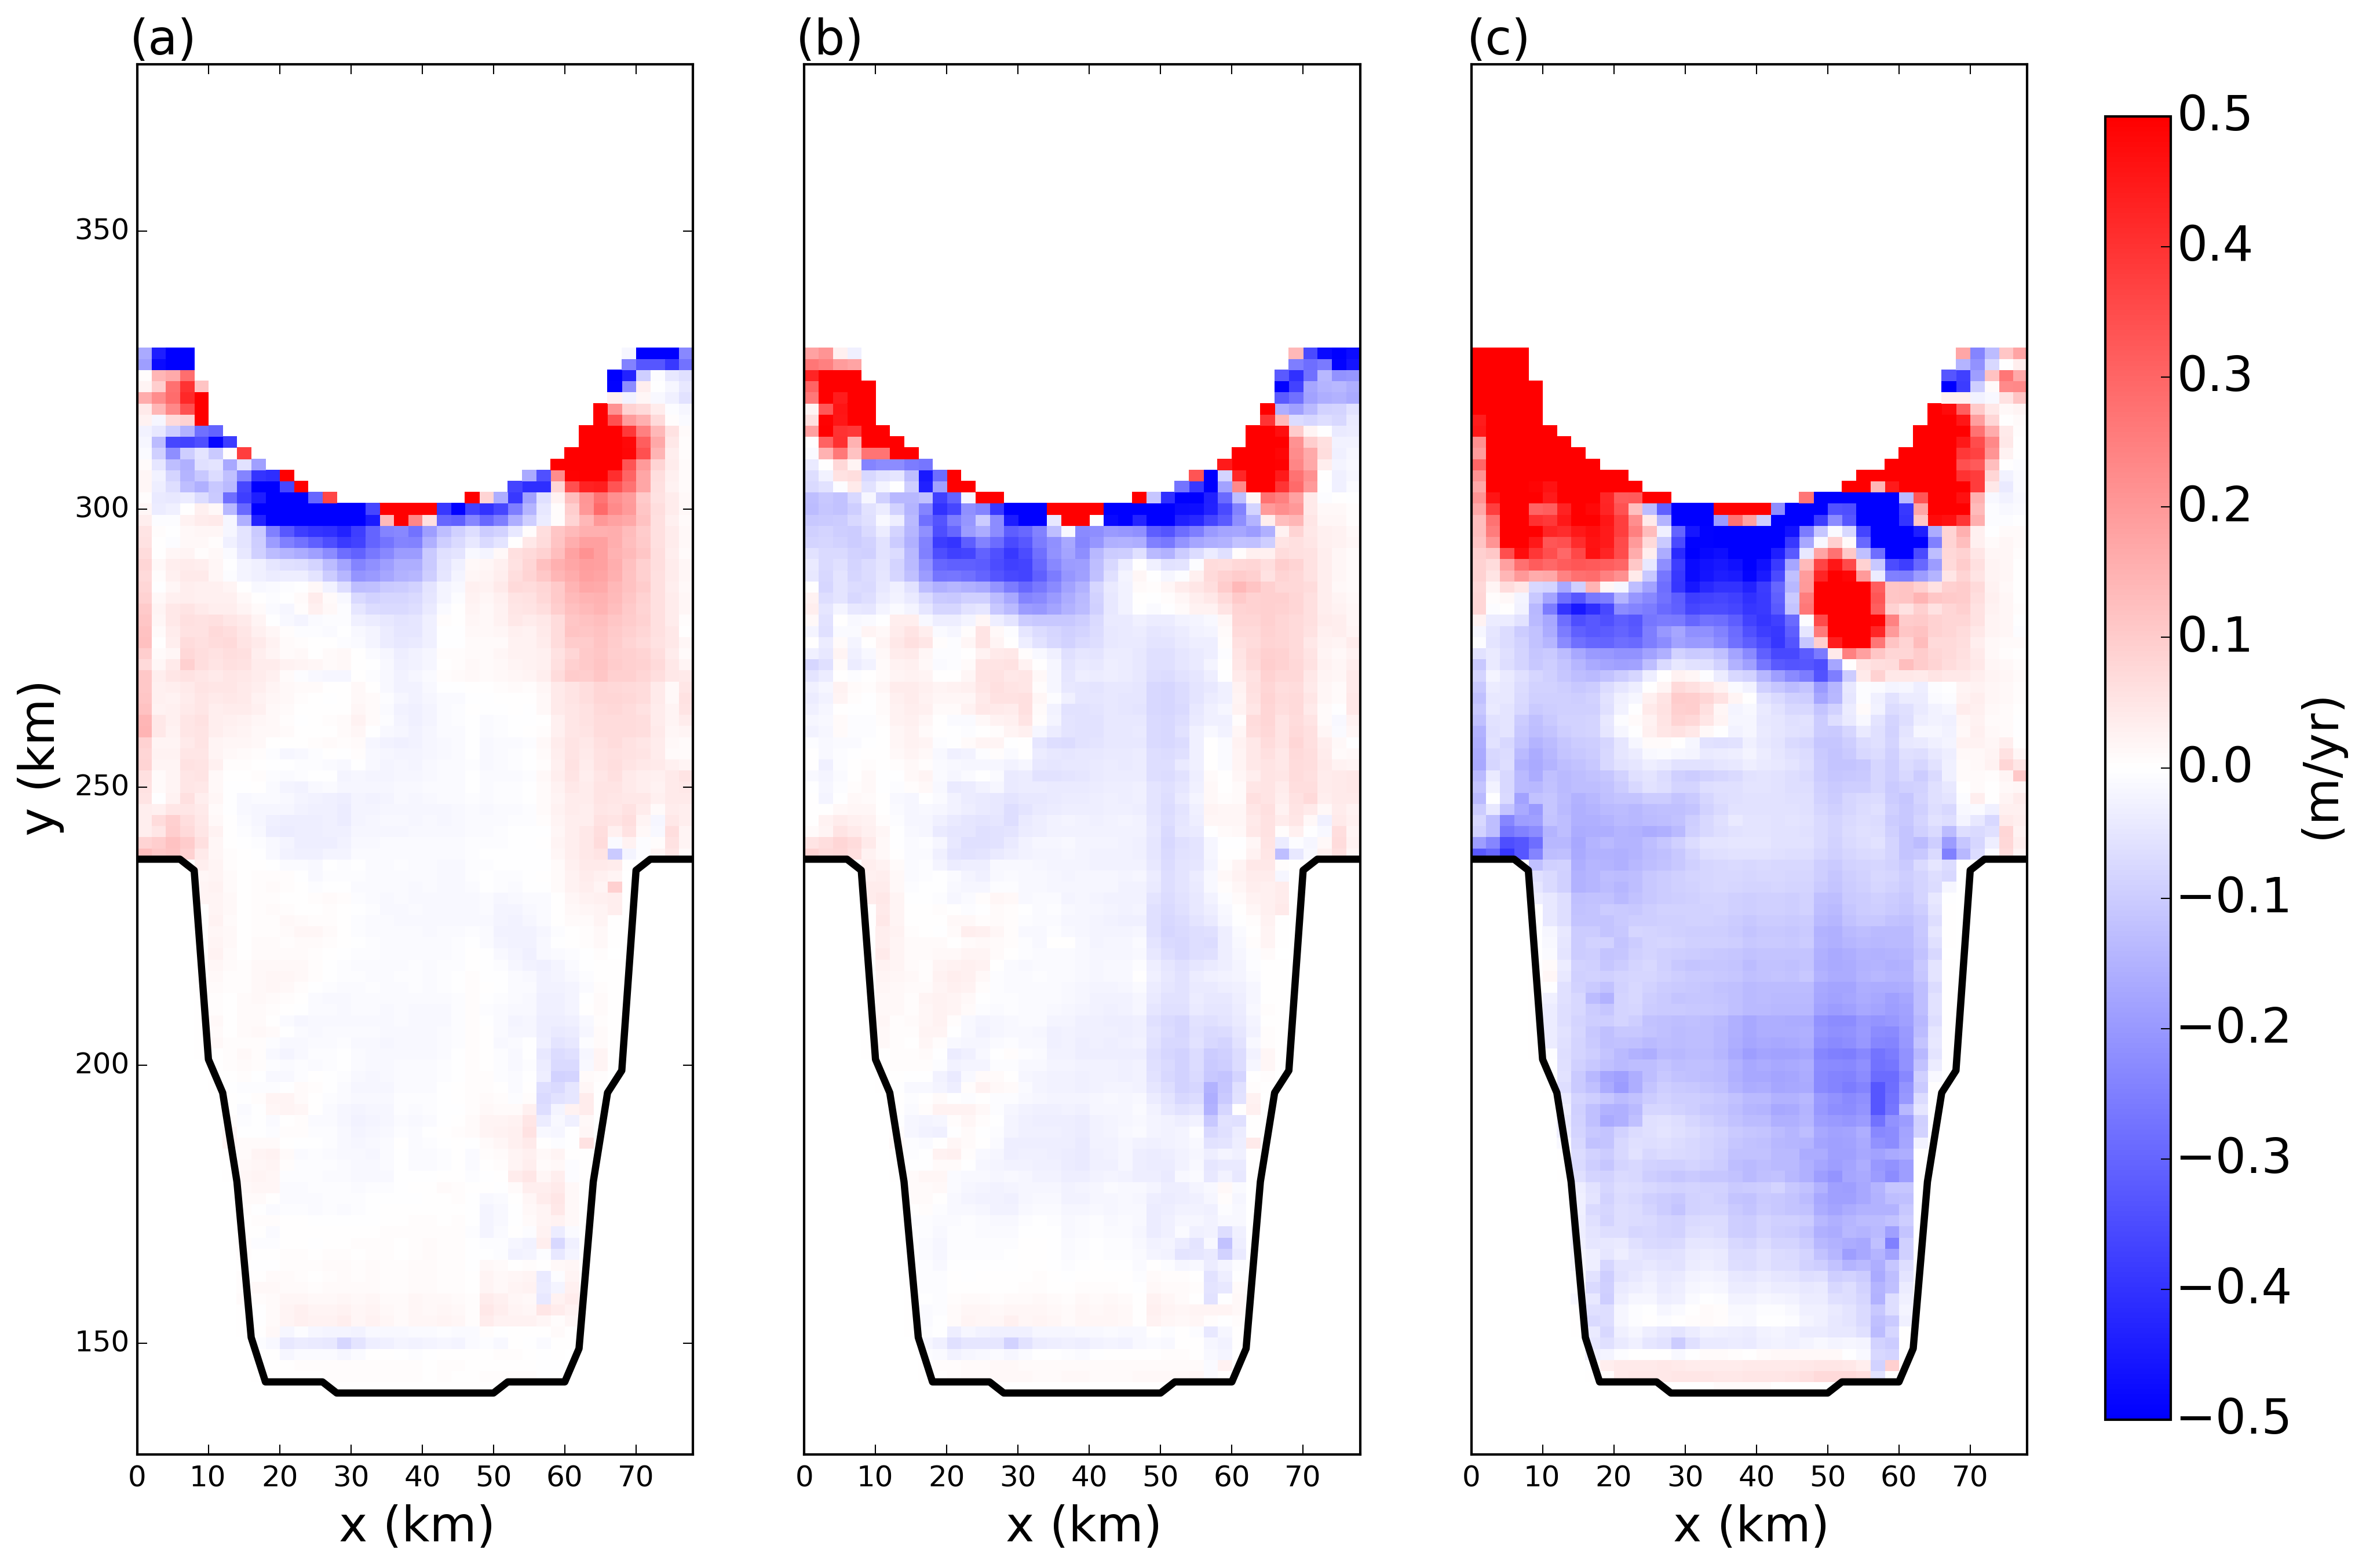
\includegraphics[width=0.99\textwidth]{Figures/snapshots_Wind_Wind_Collapse_melt_m_per_year_anomaly.png}
\caption{ { Snapshots of the melt rate anomaly, at the ice-shelf base in the tabular iceberg-calving simulation. The anomalies are relative to pre-calving melt rates.  Snapshots are taken (a) 7, (b) 15, and (c) 50 days after calving. }}
\end{center}
%FIgure created by \end{center}
\label{fig:Melt_rate_snapshots}
\end{figure}
 \clearpage
 
 
  
%\begin{figure}
%\begin{center}
%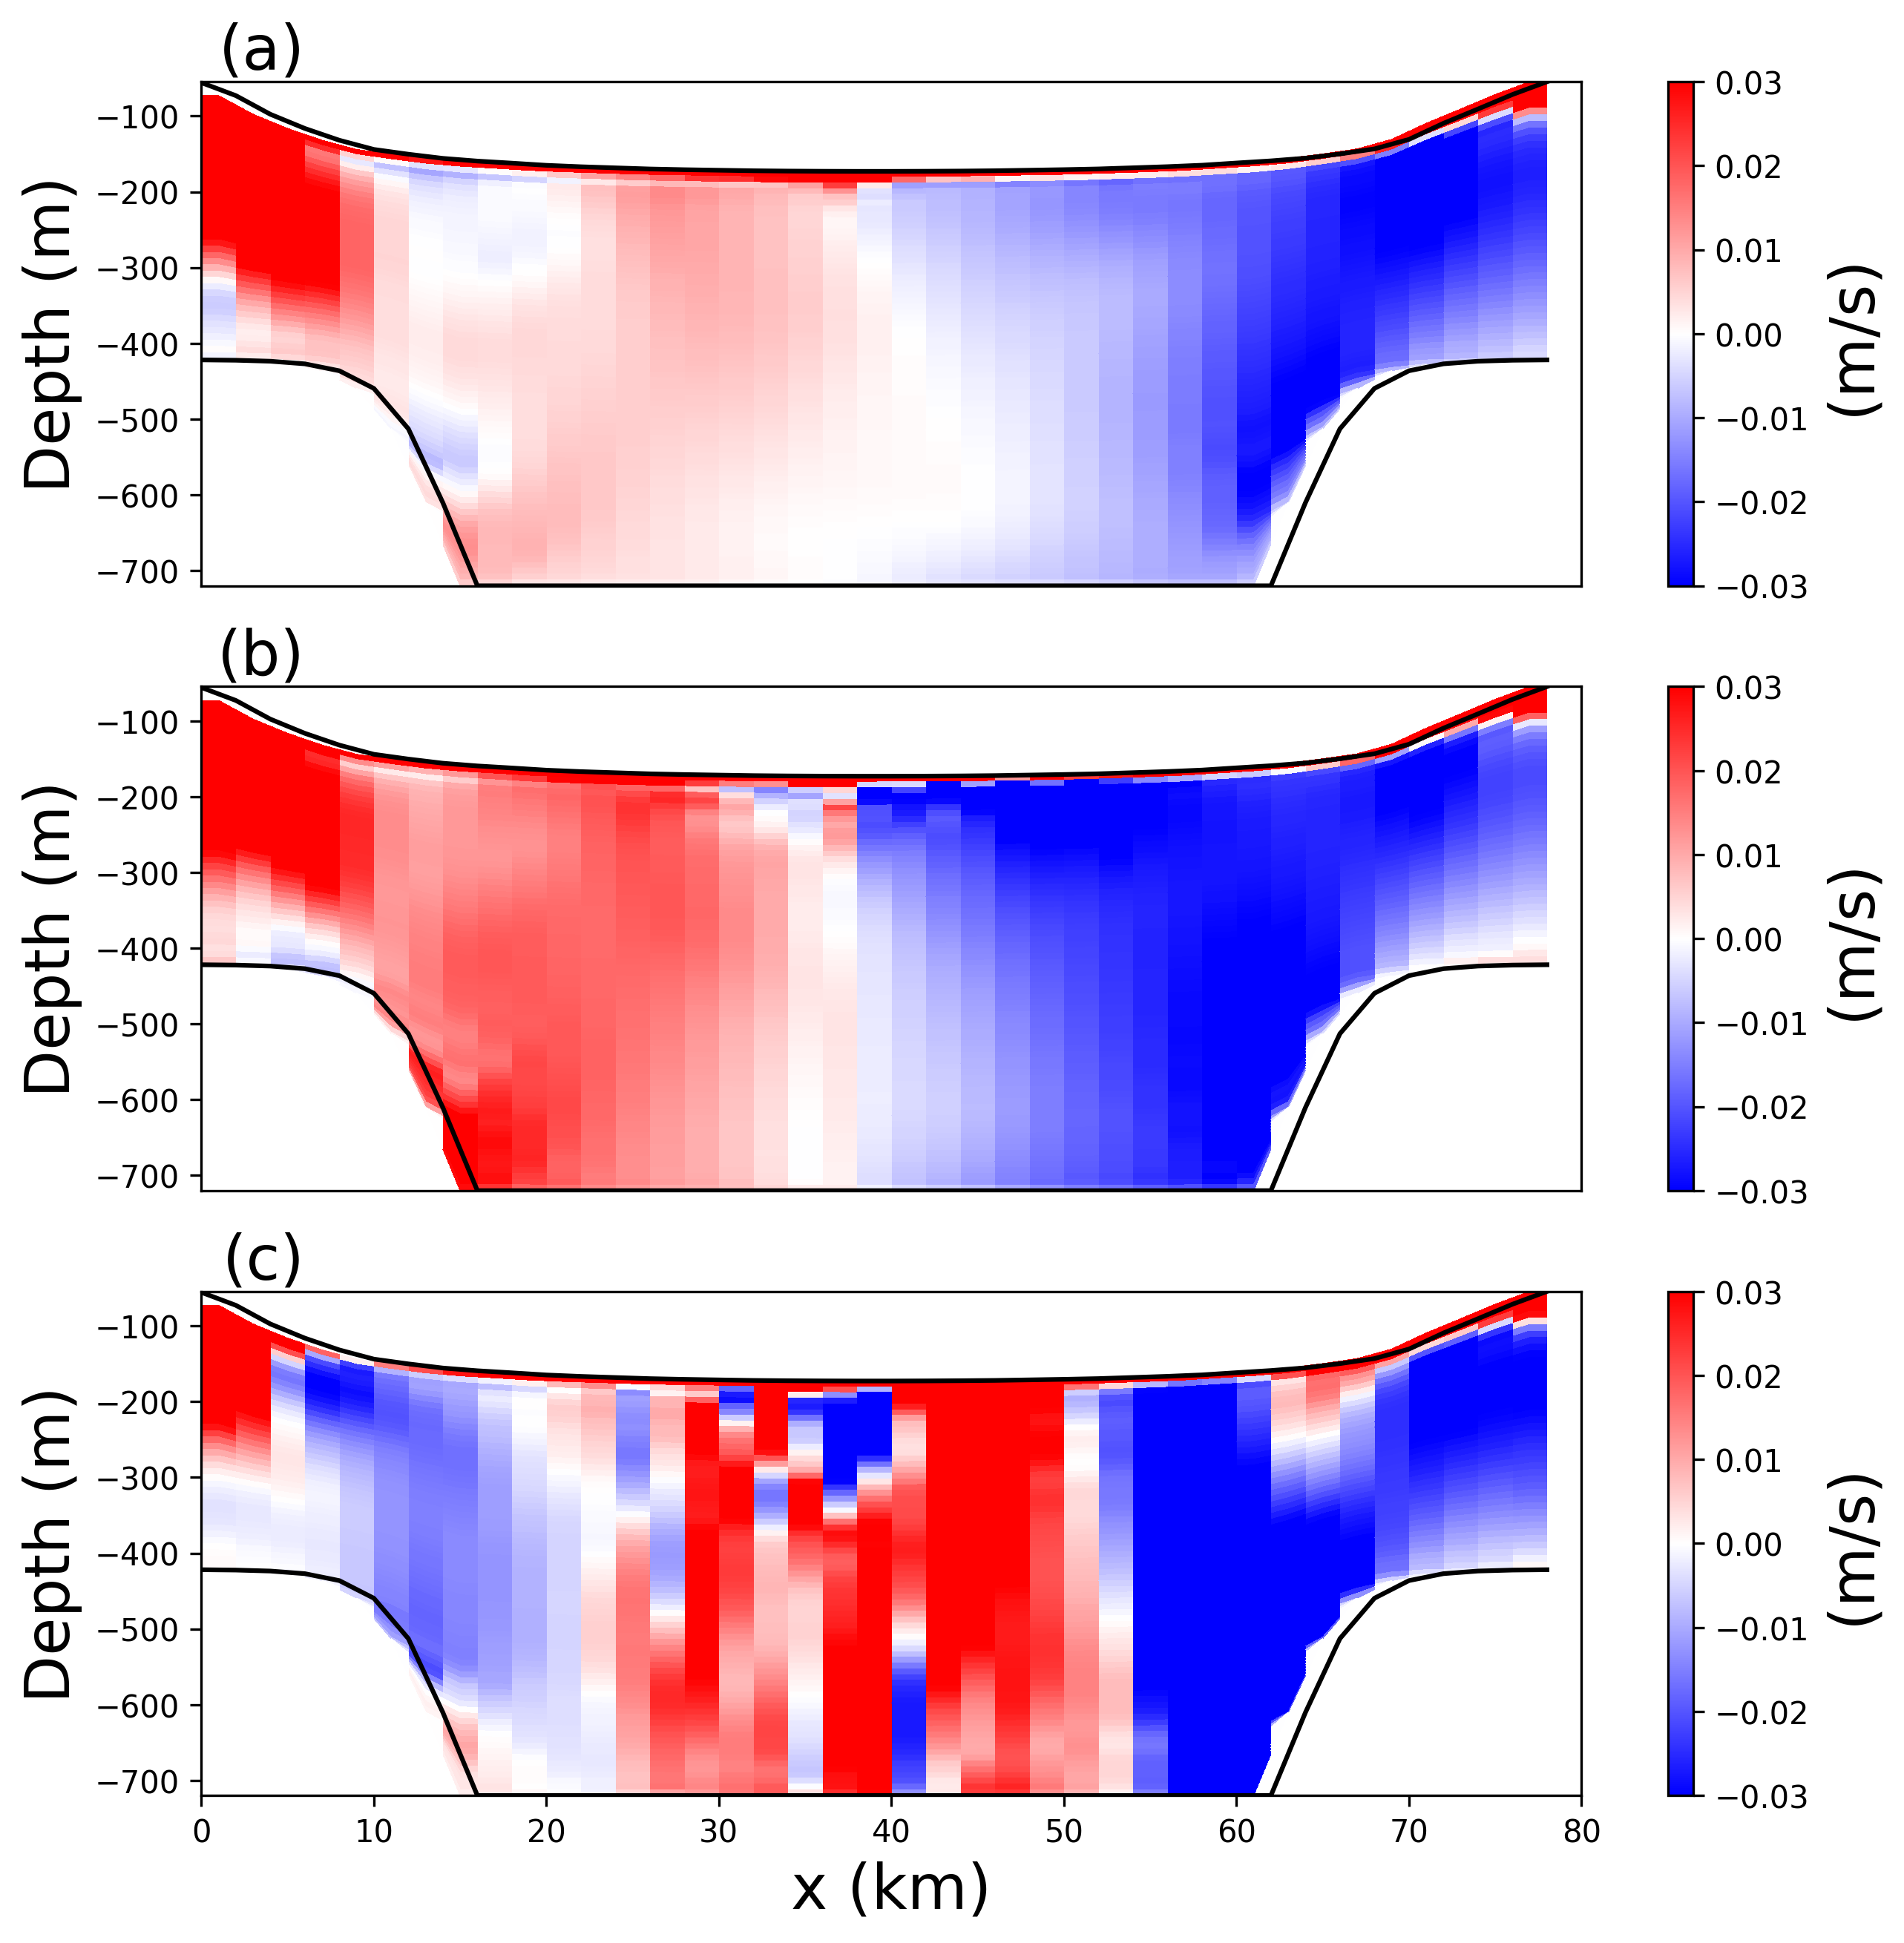
\includegraphics[width=0.99\textwidth]{Figures/snapshots_Wind_Wind_Collapse_v_layers_x149_mask_t0_t1_t50.png}
%\caption{ {Snapshots of vertical sections of meridional velocity at $y$=300~km in the tabular-iceberg-calving experiment. Snapshots are taken (a) 0, (b) 1, and (c) 50 days after calving. The position of the vertical transects is shown by the blue dashed lines in Figure \ref{fig:SST_snapshots}a. \textcolor{red}{Could show 1,14 and 50 days after calving to be consistent with the other Figures. But this figure is more interesting}}}
%\end{center}
%\label{fig:meridional_velocity_snapshots}
%\end{figure}
% \clearpage




 
  
\begin{table}[h!]
\begin{center}
\begin{tabular}{ |c c c c| }
\hline
Parameter & Symbol & Value &  Unit \\
\hline
Domain Length &  $L_{x}$ & 80  & km \\
Domain Width &  $L_{y}$ & 480  & km \\
Horizontal Resolution &  $\Delta x$ & 2  & km \\
Number of vertical layers &  $N_{l}$ & 72  & non-dim\\
Horizontal Viscosity &  $\nu_{H}$ & 6.0 & $\frac{m^{2}}{s}$ \\
Diapycnal Viscosity &  $\nu_{V} $ & $10^{-3}$ & $\frac{m^{2}}{s}$ \\
Horizontal Diffusivity & $ \epsilon_{H}$ & 1.0 & $ \frac{m^{2}}{s}$ \\
Diapycnal Diffusivity &  $\epsilon_{V} $ & $5 \times 10^{-5}$ & $\frac{m^{2}}{s}$ \\
Initial Surface Temperature &  $ T_{t}$& -1.9   & $ ^{o} C$\\
Initial Bottom Temperature &  $ T_{b}$&  1.0  & $ ^{o} C$\\
Initial Surface Salinity &  $ S_{t}$& 33.8   & psu\\
Initial Bottom Salinity &  $ S_{b}$&  34.7  & psu\\
Maximum Ocean depth &  $H_{ocean} $ & 720 & m \\
Relaxation Time of Sponge Layer &  $T_{sponge}$ & 0.1  & days\\
%Background Frictional Velocity Below Ice &  $u^{*}_{bg}$ & 0.0  & 104 \\
%Drag Coefficient Below Ice&  c_{d} & $0.0025$  & (non dim)\\
%Class 9 &  $3.9\times 10^{11}$ & 1659 & 104 \\
Time Step for Static Shelf Experiment & $dt_{Static}$ &  1000  & s\\
Time Step for Iceberg Calving Experiment & $dt_{Calving}$ &  10  & s\\
%Class 1 &  $8.8\times 10^{7}$ & 60  & 0.0026 & 40 & 2000 \\
%Class 2 &  $4.1\times 10^{8}$ & 100 & 0.0072 & 67 & 200\\
%Class 3 &  $3.3\times 10^{9}$ & 200  & 0.029 &133 & 50 \\
%Class 4 &  $1.8\times 10^{10}$& 350 &  0.12 &175  & 20 \\
%Class 5 &  $3.8\times 10^{10}$ & 500  & 0.18 &250 & 10\\
%Class 6 &  $7.5\times 10^{10}$ & 700   & 0.35 &250 & 5\\
%Class 7 &  $1.2\times 10^{11}$ & 900  & 0.56 &250  & 2 \\
%Class 8 &  $2.2\times 10^{11}$ & 1200  & 1.0&250 & 1 \\
%Class 9 &  $3.9\times 10^{11}$ & 1600 & 1.8&250 & 1  \\
%Class 10 & $7.4\times 10^{11}$ &  2200 & 3.5 &250  &1\\
\hline
\end{tabular}
%\caption{Description of the iceberg calving classes used in the model. {\it Mass}, {\it Length}, {\it Area} and {\it Th} refer to the iceberg mass, length, area, and thickness at the time of calving.  {\it Scaling} is the number of icebergs represented by one Lagrangian point particle. The iceberg mass and thickness for each class are the same as those reported in \citet{Gladstone2001}. The iceberg area and length for each class is calculated from the iceberg mass and thickness by assuming that the icebergs are cuboids with a length to width ratio of 1.5, using an iceberg density $\rho_{i}=850$kg/$\textrm{m}^{3}$.}
% Note that the areas of the iceberg classes (calculated from the iceberg lengths and masses given in \citep{Gladstone2001}) are not monotonically increasing.
\label{table:parameters2}
\end{center}
\end{table}

\clearpage

%\begin{figure}
%\begin{center}
%\includegraphics[width=0.99\textwidth]{Figures/fixed_drift_bond_Iceberg_calving.png}
%\caption{ {Need to update this Figure. Also, I should try using orientation with the Bonds.}}
%\end{center}
%FIgure created by \end{center}
%\label{fig:}
%\end{figure}


% \clearpage

%\begin{figure}
%\begin{center}
%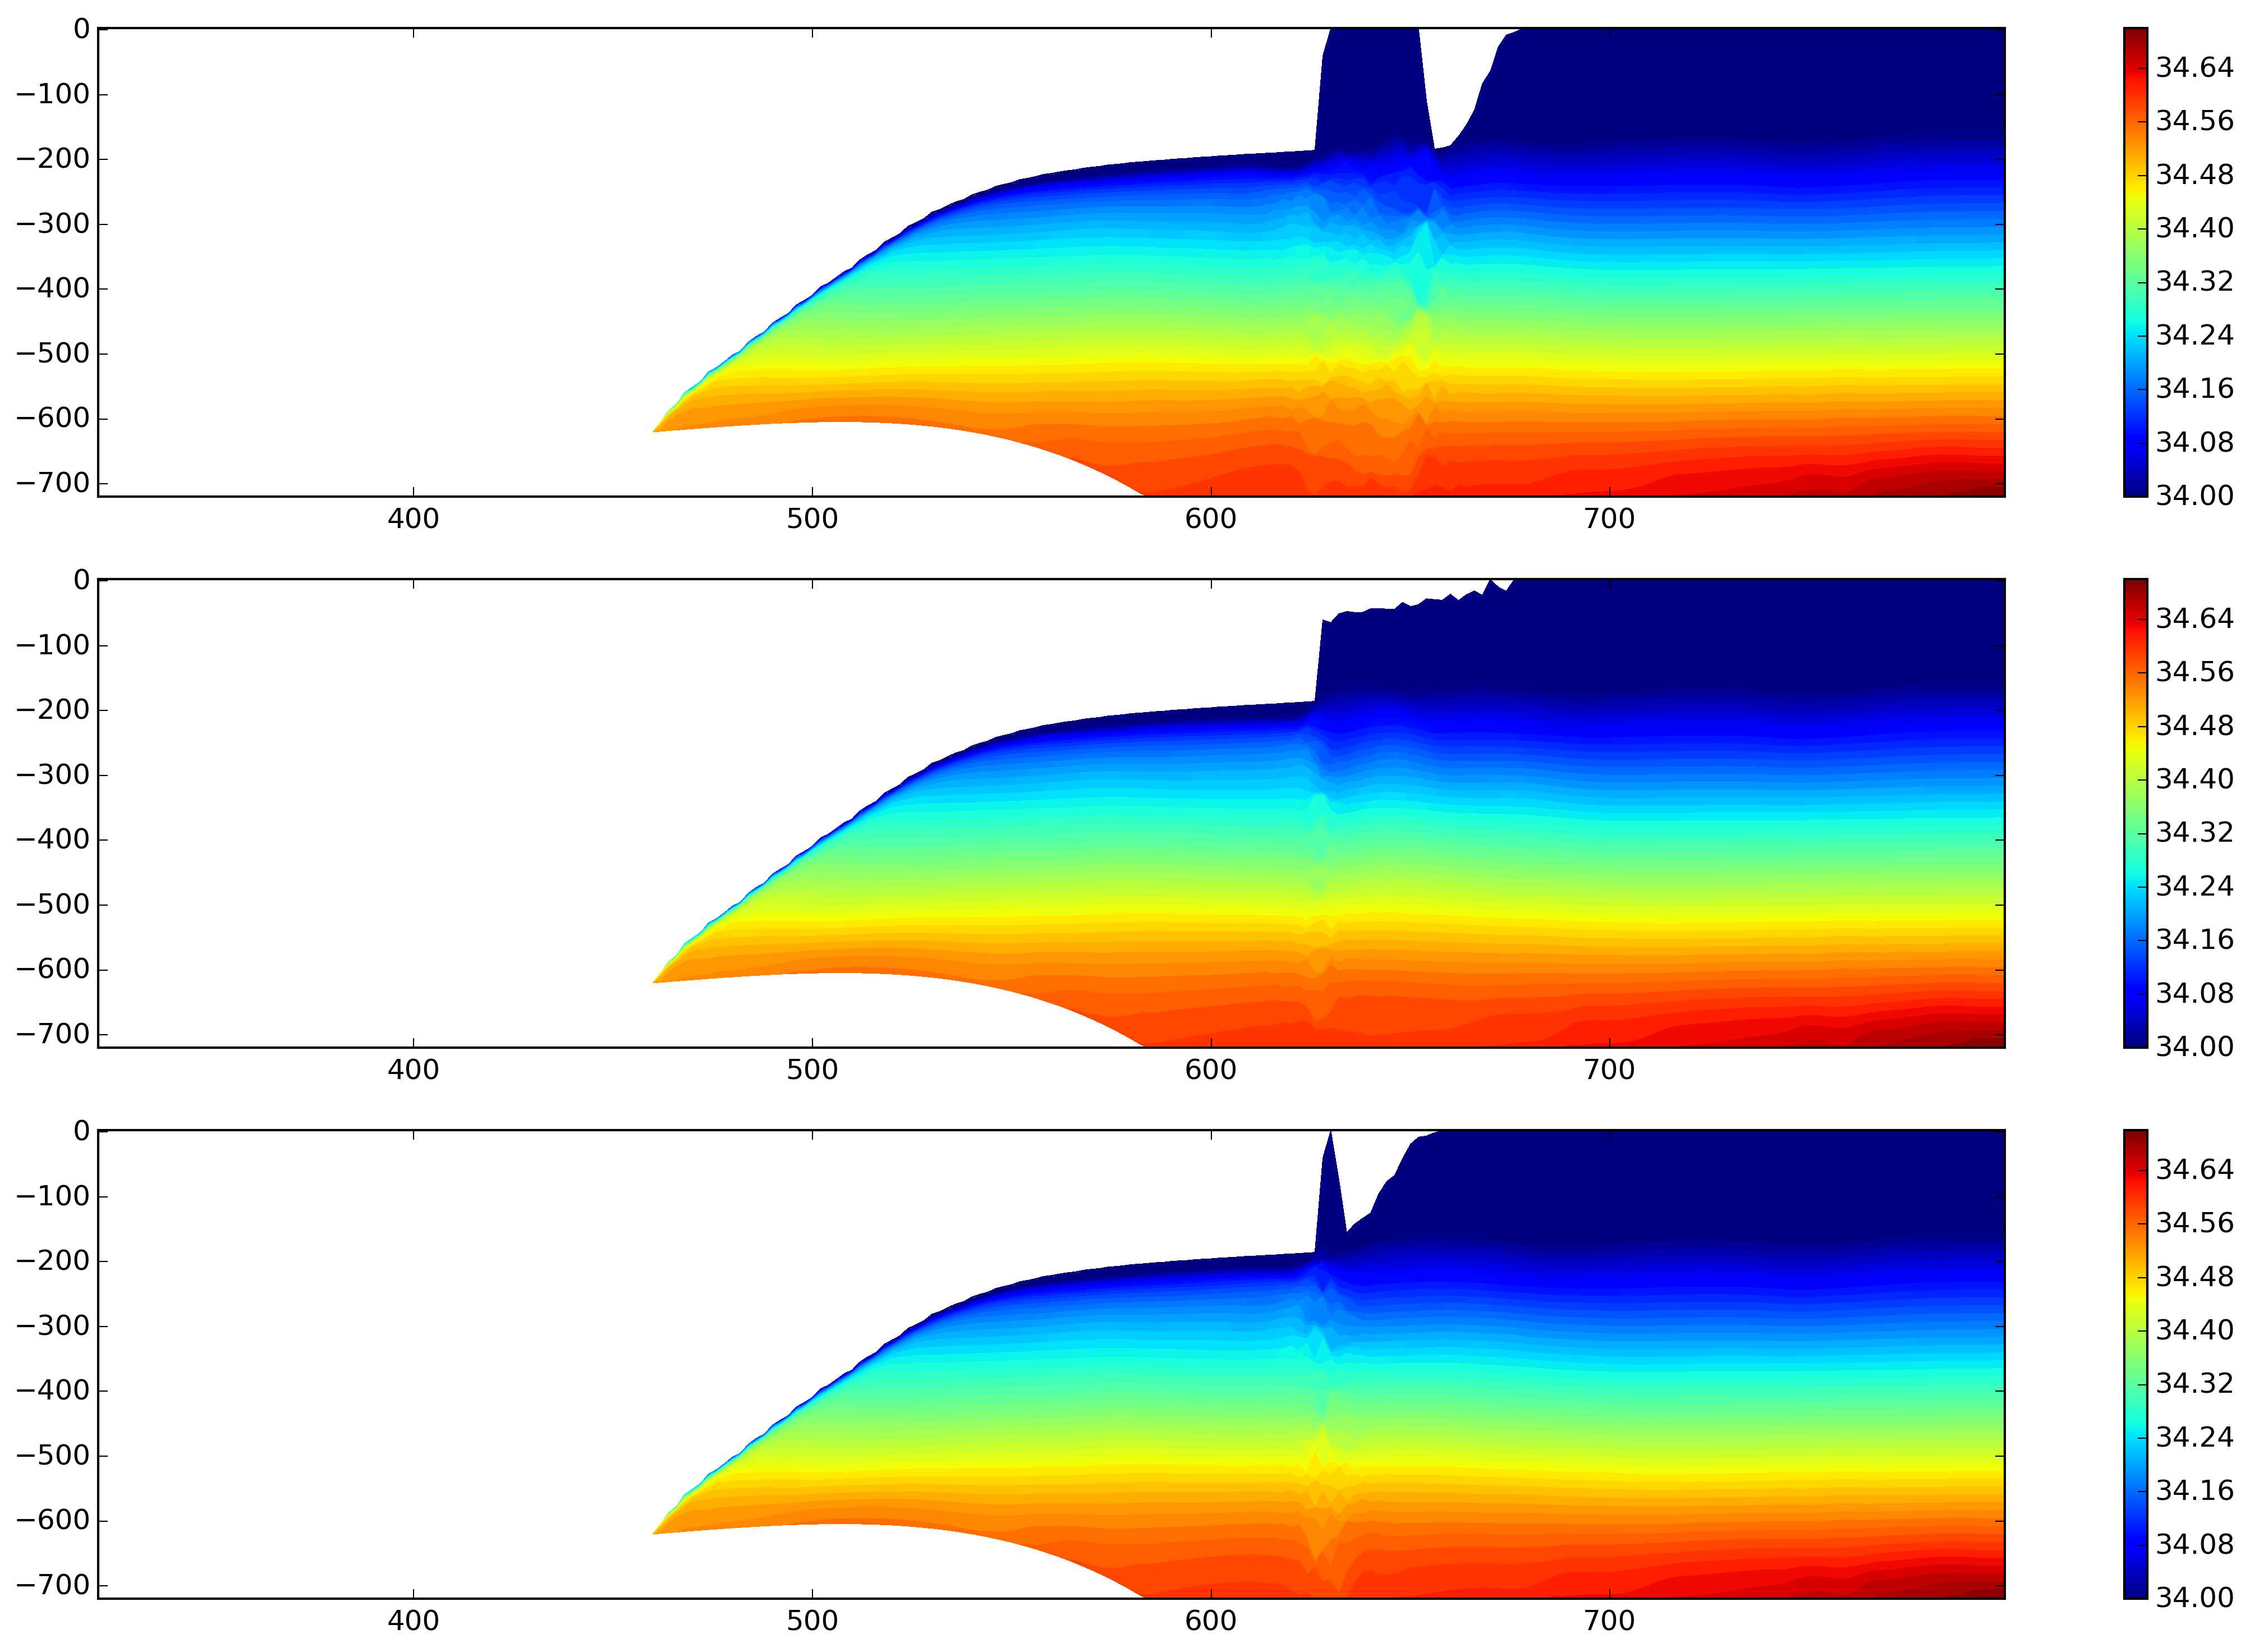
\includegraphics[width=0.99\textwidth]{Figures/fixed_drift_bond_salt_layers.png}
%\caption{ {}}
%\end{center}
%FIgure created by \end{center}
%\label{fig:}
%\end{figure}

%\clearpage

%\begin{figure}
%\begin{center}
%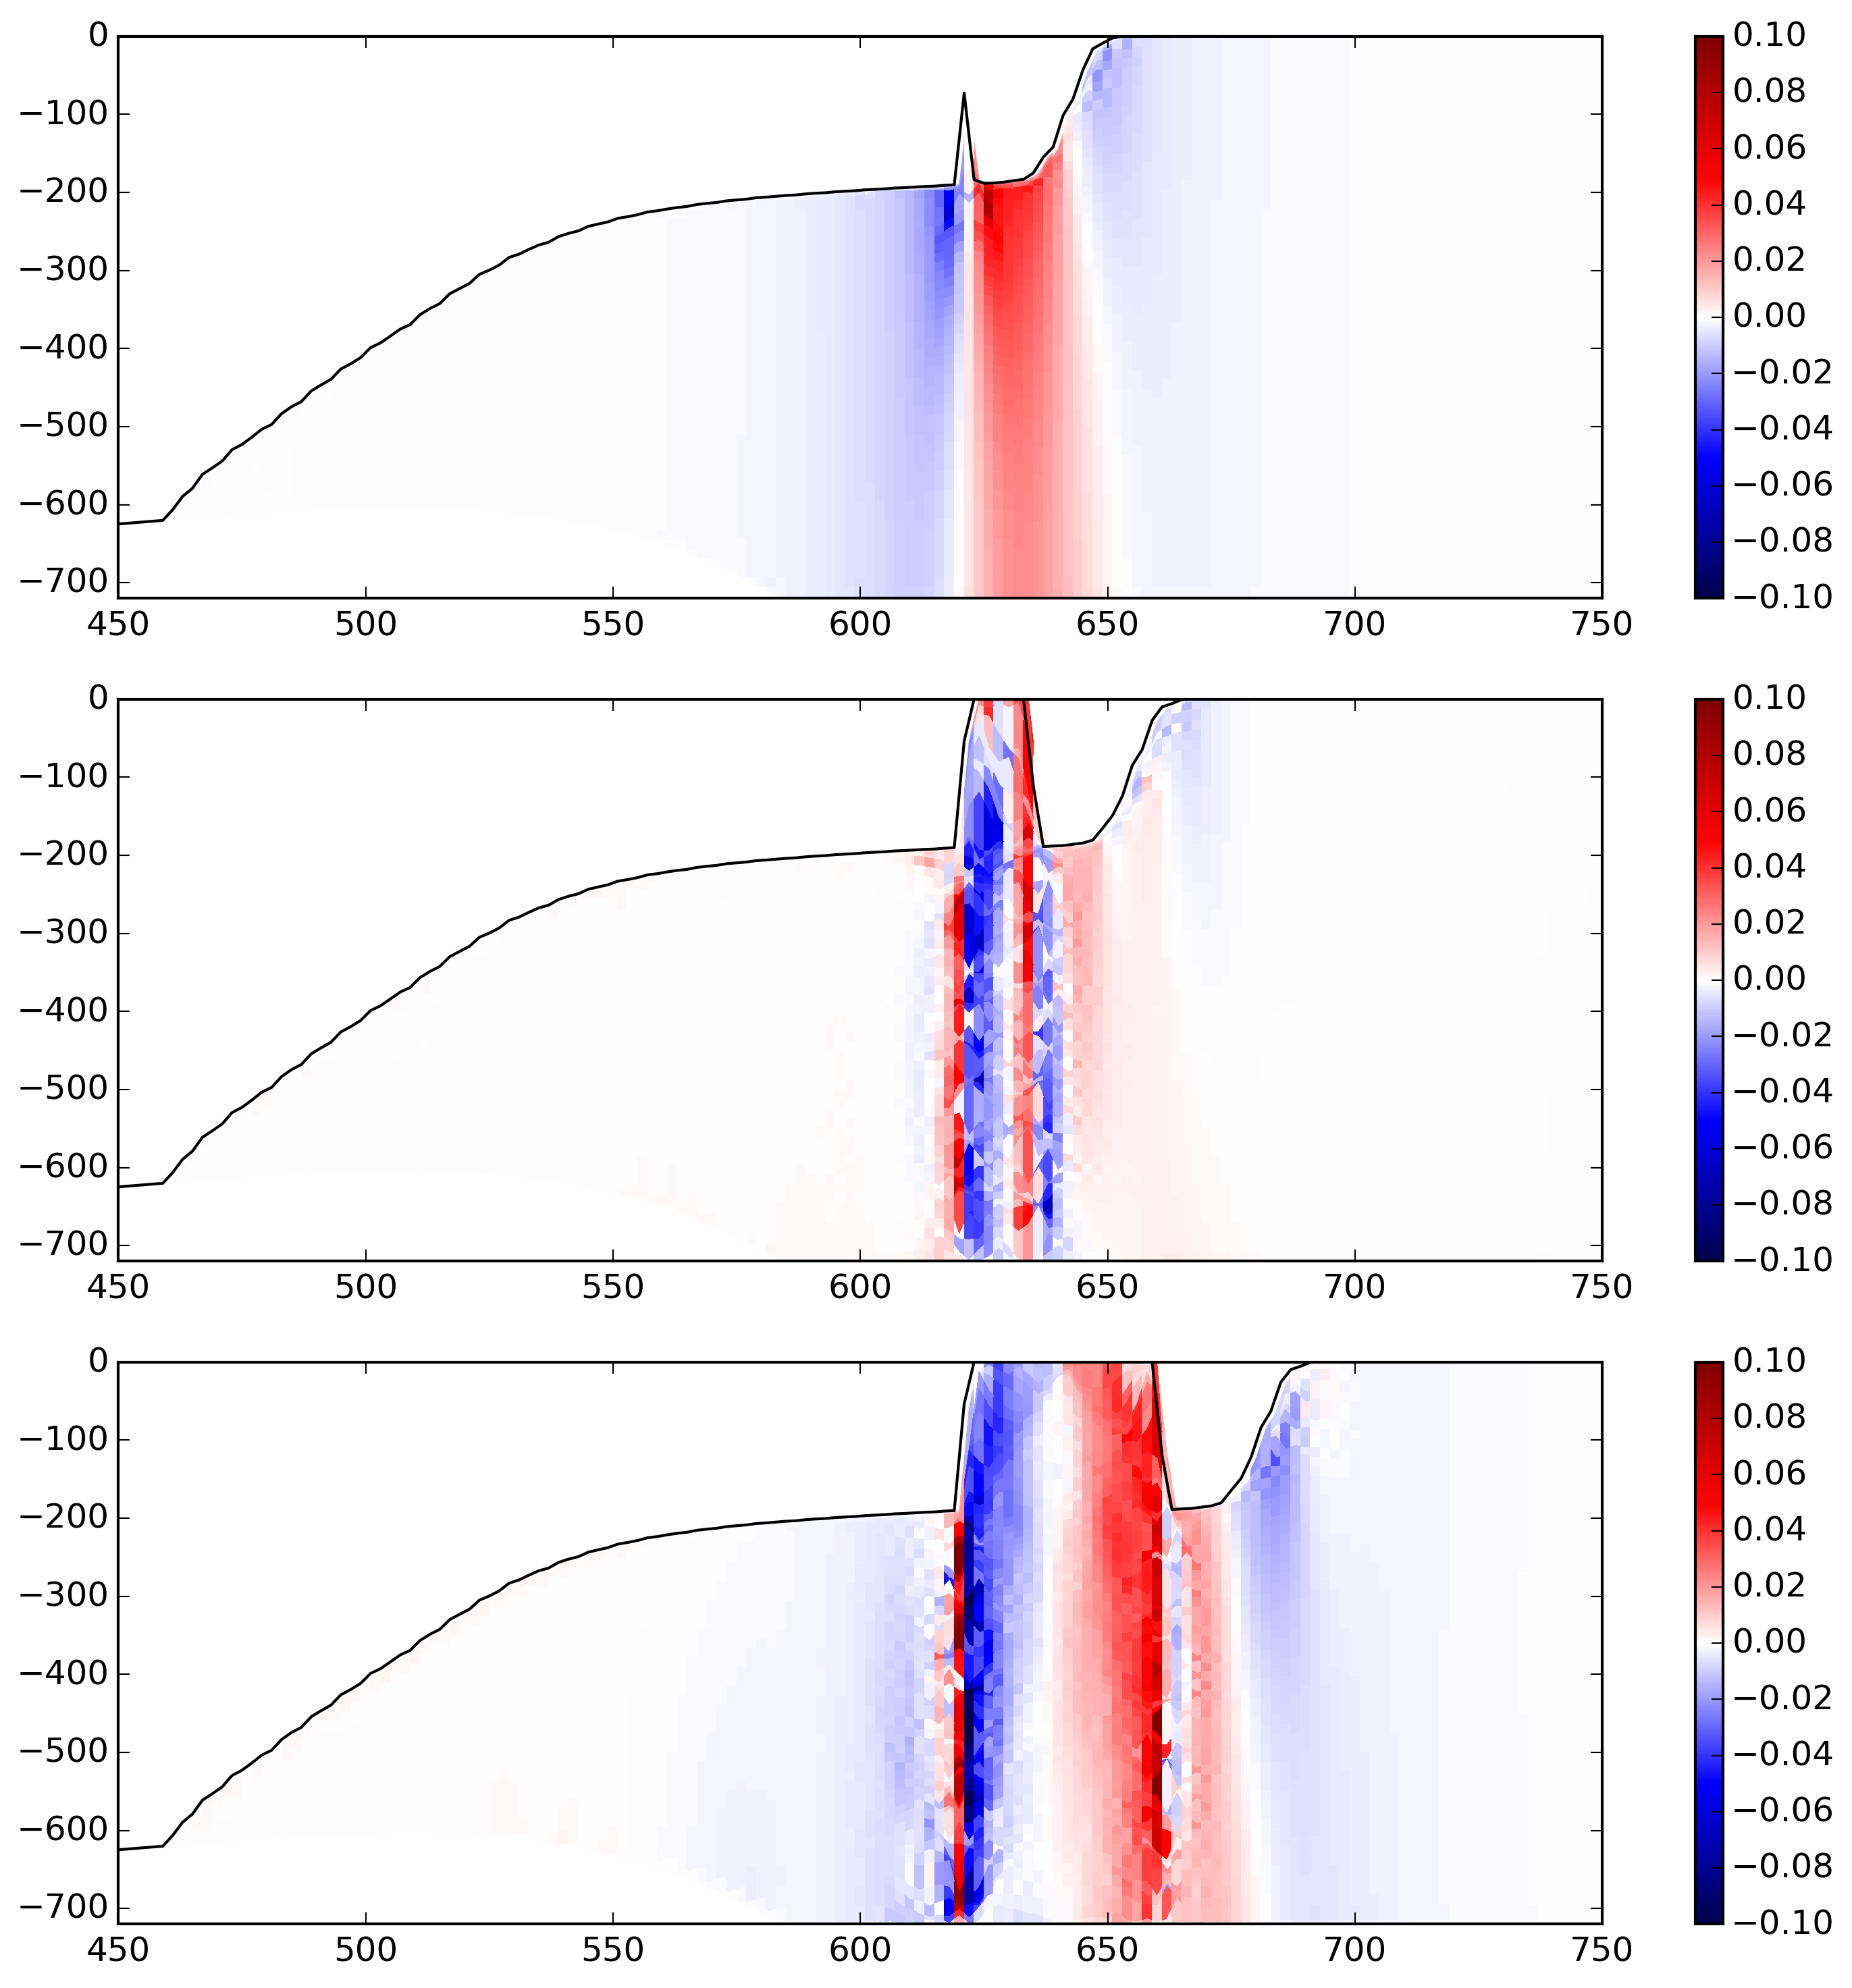
\includegraphics[width=0.99\textwidth]{Figures/snapshots_fixed_01_u_layers.png}
%\caption{ {Need to update this Figure. }}
%\end{center}
%FIgure created by \end{center}
%\label{fig:}
%\end{figure}


%\clearpage

%\begin{figure}
%\begin{center}
%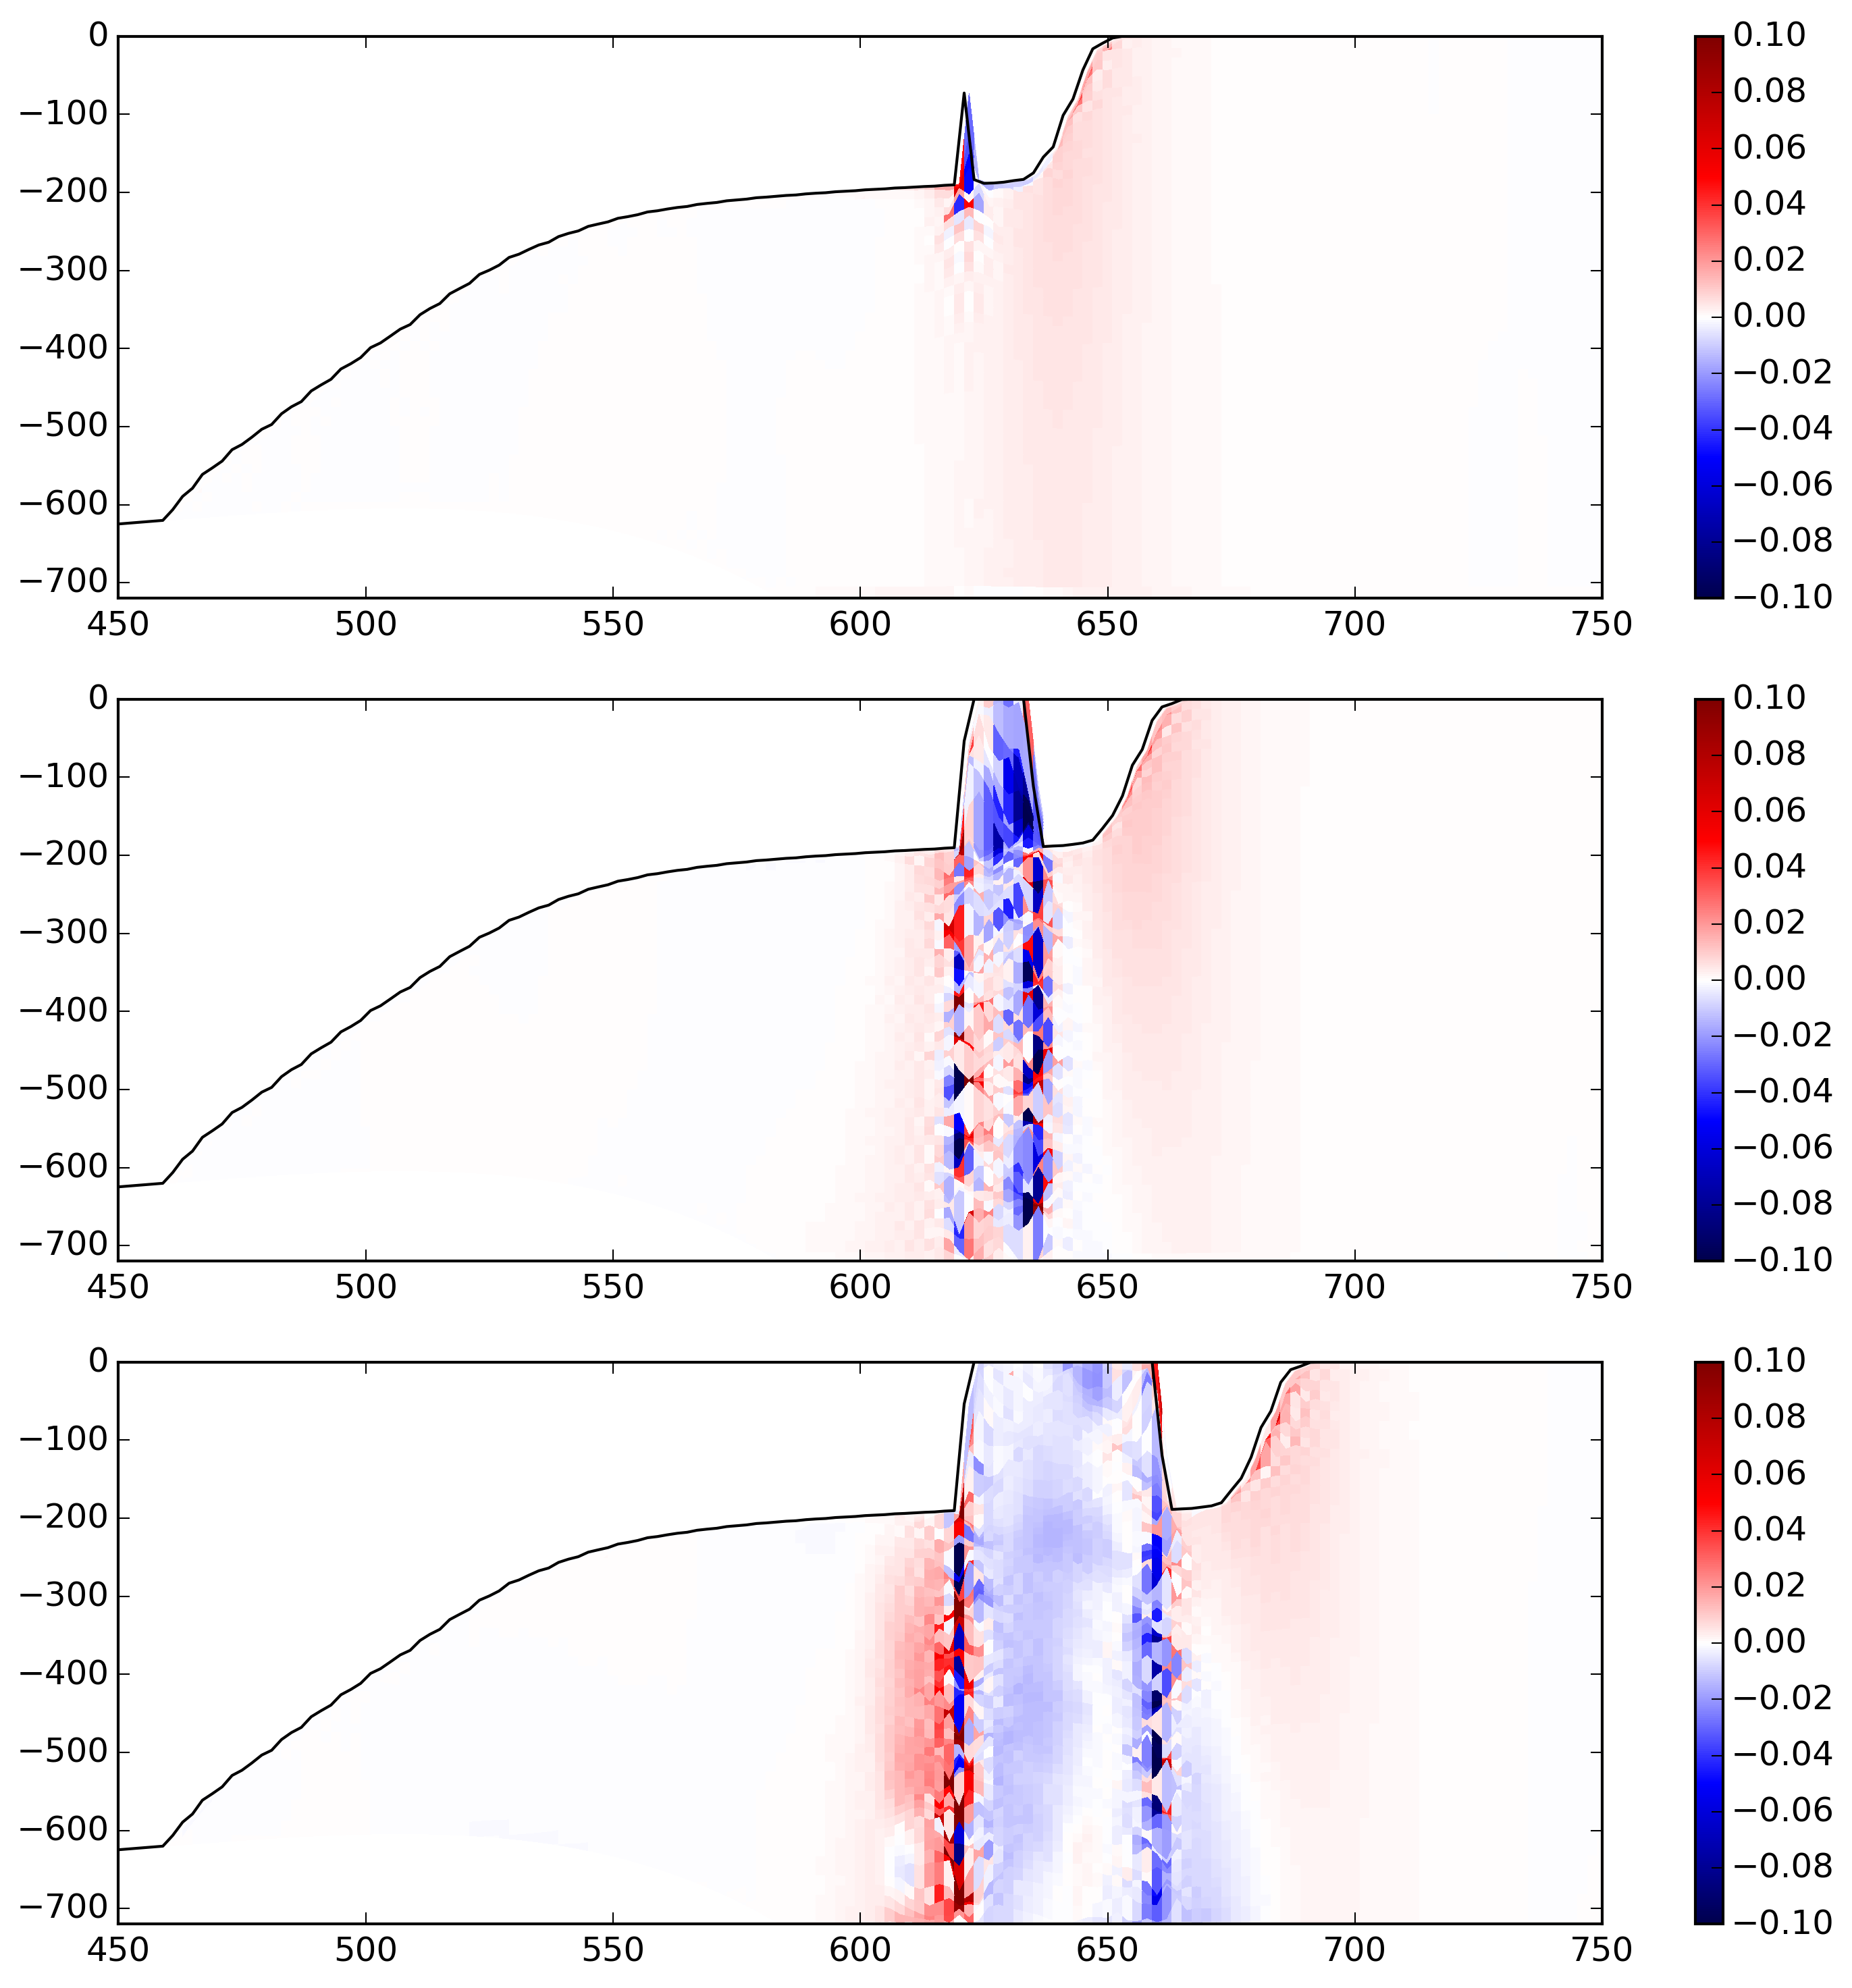
\includegraphics[width=0.99\textwidth]{Figures/snapshots_fixed_01_v_layers.png}
%\caption{ {Need to update this Figure. }}
%\end{center}
%FIgure created by \end{center}
%\label{fig:}
%\end{figure}



%%%%%%%%%%%%%%%%%%%%%%%%%%%%%%%%%%%%%%%%%%%%%%%%%%%%%%%%%%%%%%%%%%%%%%%%%%%%%%%%%%%%%
%%%%%%%%%%%%%%%%%%%%%%%%%%%%%%%%%%%%%%%%%%%%%%%%%%%%%%%%%%%%%%%%%%%%%%%%%%%%%%%%%%%%%
%%%%%%%%%%%%%%%%%%%%%%%%%%%%%%%%%%%%%%%%%%%%%%%%%%%%%%%%%%%%%%%%%%%%%%%%%%%%%%%%%%%%%
%%%%%%%%%%%%%%%%%%%%%%%%%%%%%%%%%%%%%%%%%%%%%%%%%%%%%%%%%%%%%%%%%%%%%%%%%%%%%%%%%%%%%
%%%%%%%%%%%%%%%%%%%%%%%%%%%%%%%%%%%%%%%%%%%%%%%%%%%%%%%%%%%%%%%%%%%%%%%%%%%%%%%%%%%%%
%%%%%%%%%%%%%%%%%%%%%%%%%%%%%%%%%%%%%%%%%%%%%%%%%%%%%%%%%%%%%%%%%%%%%%%%%%%%%%%%%%%%%
%%%%%%%%%%%%%%%%%%%%%%%%%%%%%%%%%%%%%%%%%%%%%%%%%%%%%%%%%%%%%%%%%%%%%%%%%%%%%%%%%%%%%
%%%%%%%%%%%%%%%%%%%%%%%%%%%%%%%%%%%%%%%%%%%%%%%%%%%%%%%%%%%%%%%%%%%%%%%%%%%%%%%%%%%%%
%%%%%%%%%%%%%%%%%%%%%%%%%%%%%%%%%%%%%%%%%%%%%%%%%%%%%%%%%%%%%%%%%%%%%%%%%%%%%%%%%%%%%
%%%%%%%%%%%%%%%%%%%%%%%%%%%%%%%%%%%%%%%%%%%%%%%%%%%%%%%%%%%%%%%%%%%%%%%%%%%%%%%%%%%%%
%%%%%%%%%%%%%%%%%%%%%%%%%%%                       Supplementary Figures                   %%%%%%%%%%%%%%%%%%%%%%%%%%%%%%%%%
%%%%%%%%%%%%%%%%%%%%%%%%%%%%%%%%%%%%%%%%%%%%%%%%%%%%%%%%%%%%%%%%%%%%%%%%%%%%%%%%%%%%%
%%%%%%%%%%%%%%%%%%%%%%%%%%%%%%%%%%%%%%%%%%%%%%%%%%%%%%%%%%%%%%%%%%%%%%%%%%%%%%%%%%%%%
%%%%%%%%%%%%%%%%%%%%%%%%%%%%%%%%%%%%%%%%%%%%%%%%%%%%%%%%%%%%%%%%%%%%%%%%%%%%%%%%%%%%%
%%%%%%%%%%%%%%%%%%%%%%%%%%%%%%%%%%%%%%%%%%%%%%%%%%%%%%%%%%%%%%%%%%%%%%%%%%%%%%%%%%%%%
%%%%%%%%%%%%%%%%%%%%%%%%%%%%%%%%%%%%%%%%%%%%%%%%%%%%%%%%%%%%%%%%%%%%%%%%%%%%%%%%%%%%%
%%%%%%%%%%%%%%%%%%%%%%%%%%%%%%%%%%%%%%%%%%%%%%%%%%%%%%%%%%%%%%%%%%%%%%%%%%%%%%%%%%%%%
%%%%%%%%%%%%%%%%%%%%%%%%%%%%%%%%%%%%%%%%%%%%%%%%%%%%%%%%%%%%%%%%%%%%%%%%%%%%%%%%%%%%%
%%%%%%%%%%%%%%%%%%%%%%%%%%%%%%%%%%%%%%%%%%%%%%%%%%%%%%%%%%%%%%%%%%%%%%%%%%%%%%%%%%%%%
%%%%%%%%%%%%%%%%%%%%%%%%%%%%%%%%%%%%%%%%%%%%%%%%%%%%%%%%%%%%%%%%%%%%%%%%%%%%%%%%%%%%%
%%%%%%%%%%%%%%%%%%%%%%%%%%%%%%%%%%%%%%%%%%%%%%%%%%%%%%%%%%%%%%%%%%%%%%%%%%%%%%%%%%%%%
%%%%%%%%%%%%%%%%%%%%%%%%%%%%%%%%%%%%%%%%%%%%%%%%%%%%%%%%%%%%%%%%%%%%%%%%%%%%%%%%%%%%%

\clearpage
\section{Supplementary Figures}
\clearpage

\setcounter{figure}{0}
\renewcommand{\thefigure}{S\arabic{figure}}



\begin{figure}
\begin{center}
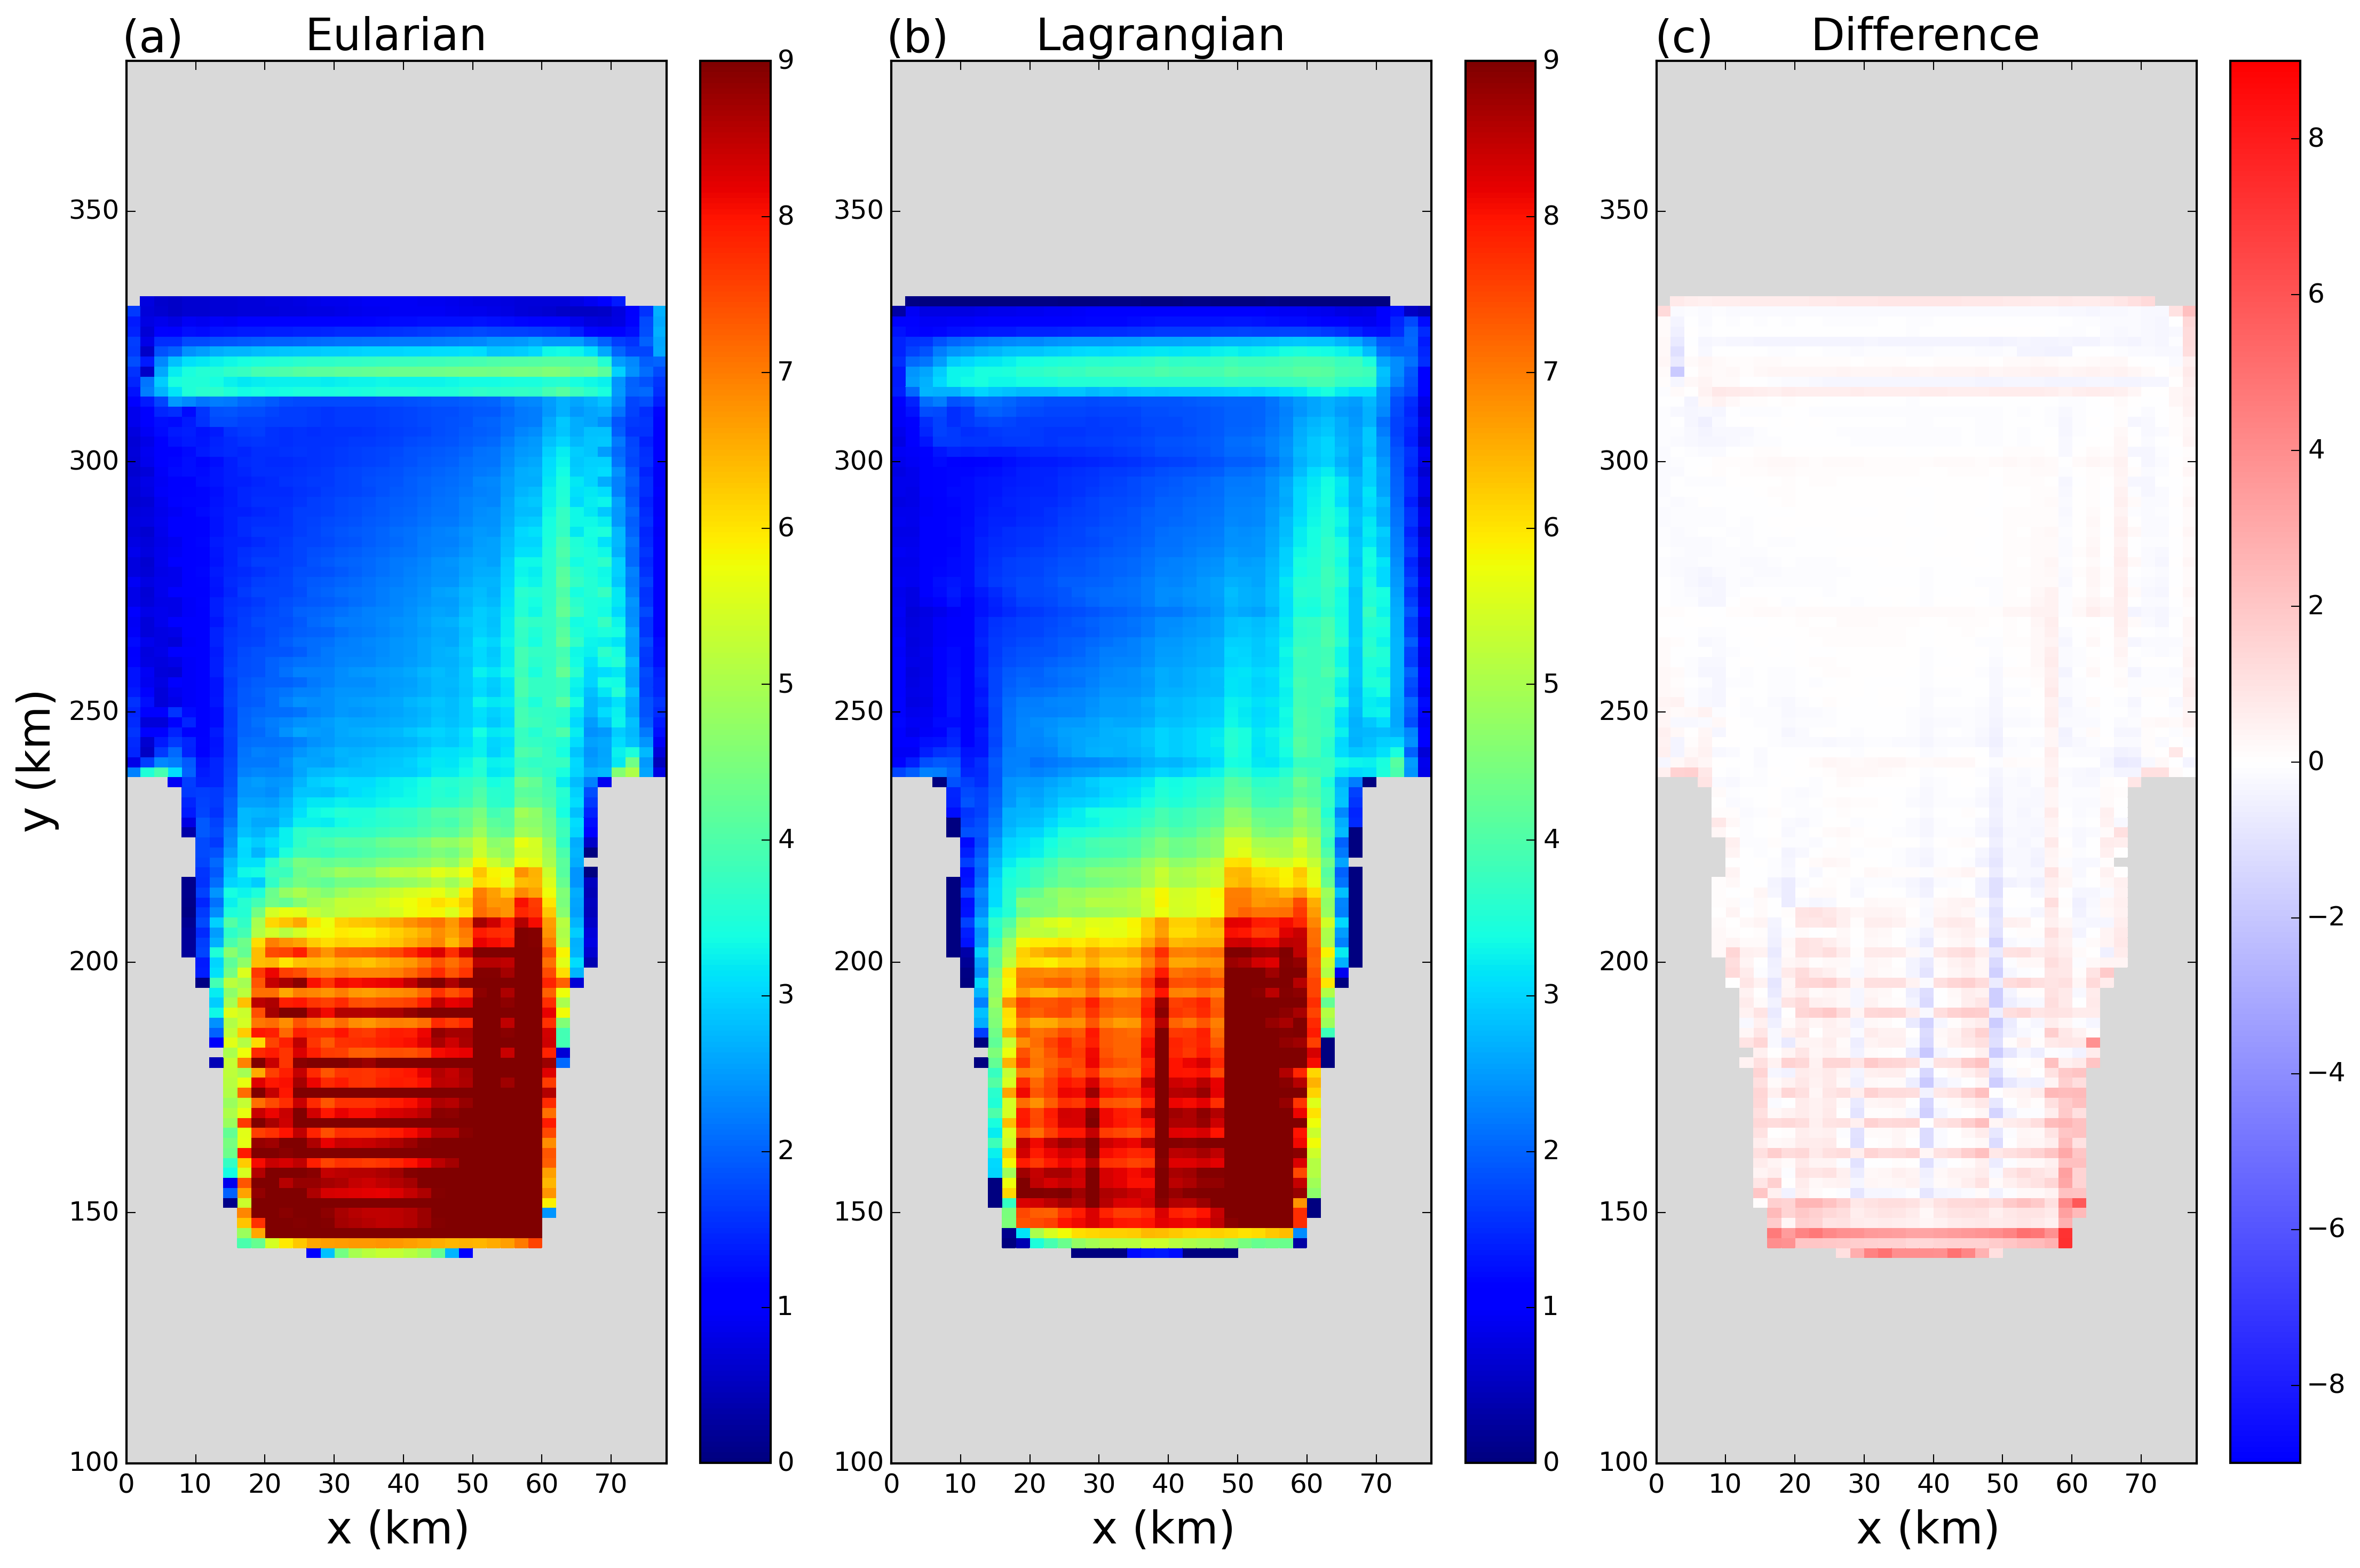
\includegraphics[width=0.99\textwidth]{Figures/Wind_static_shelf_comparison_melt.png}
%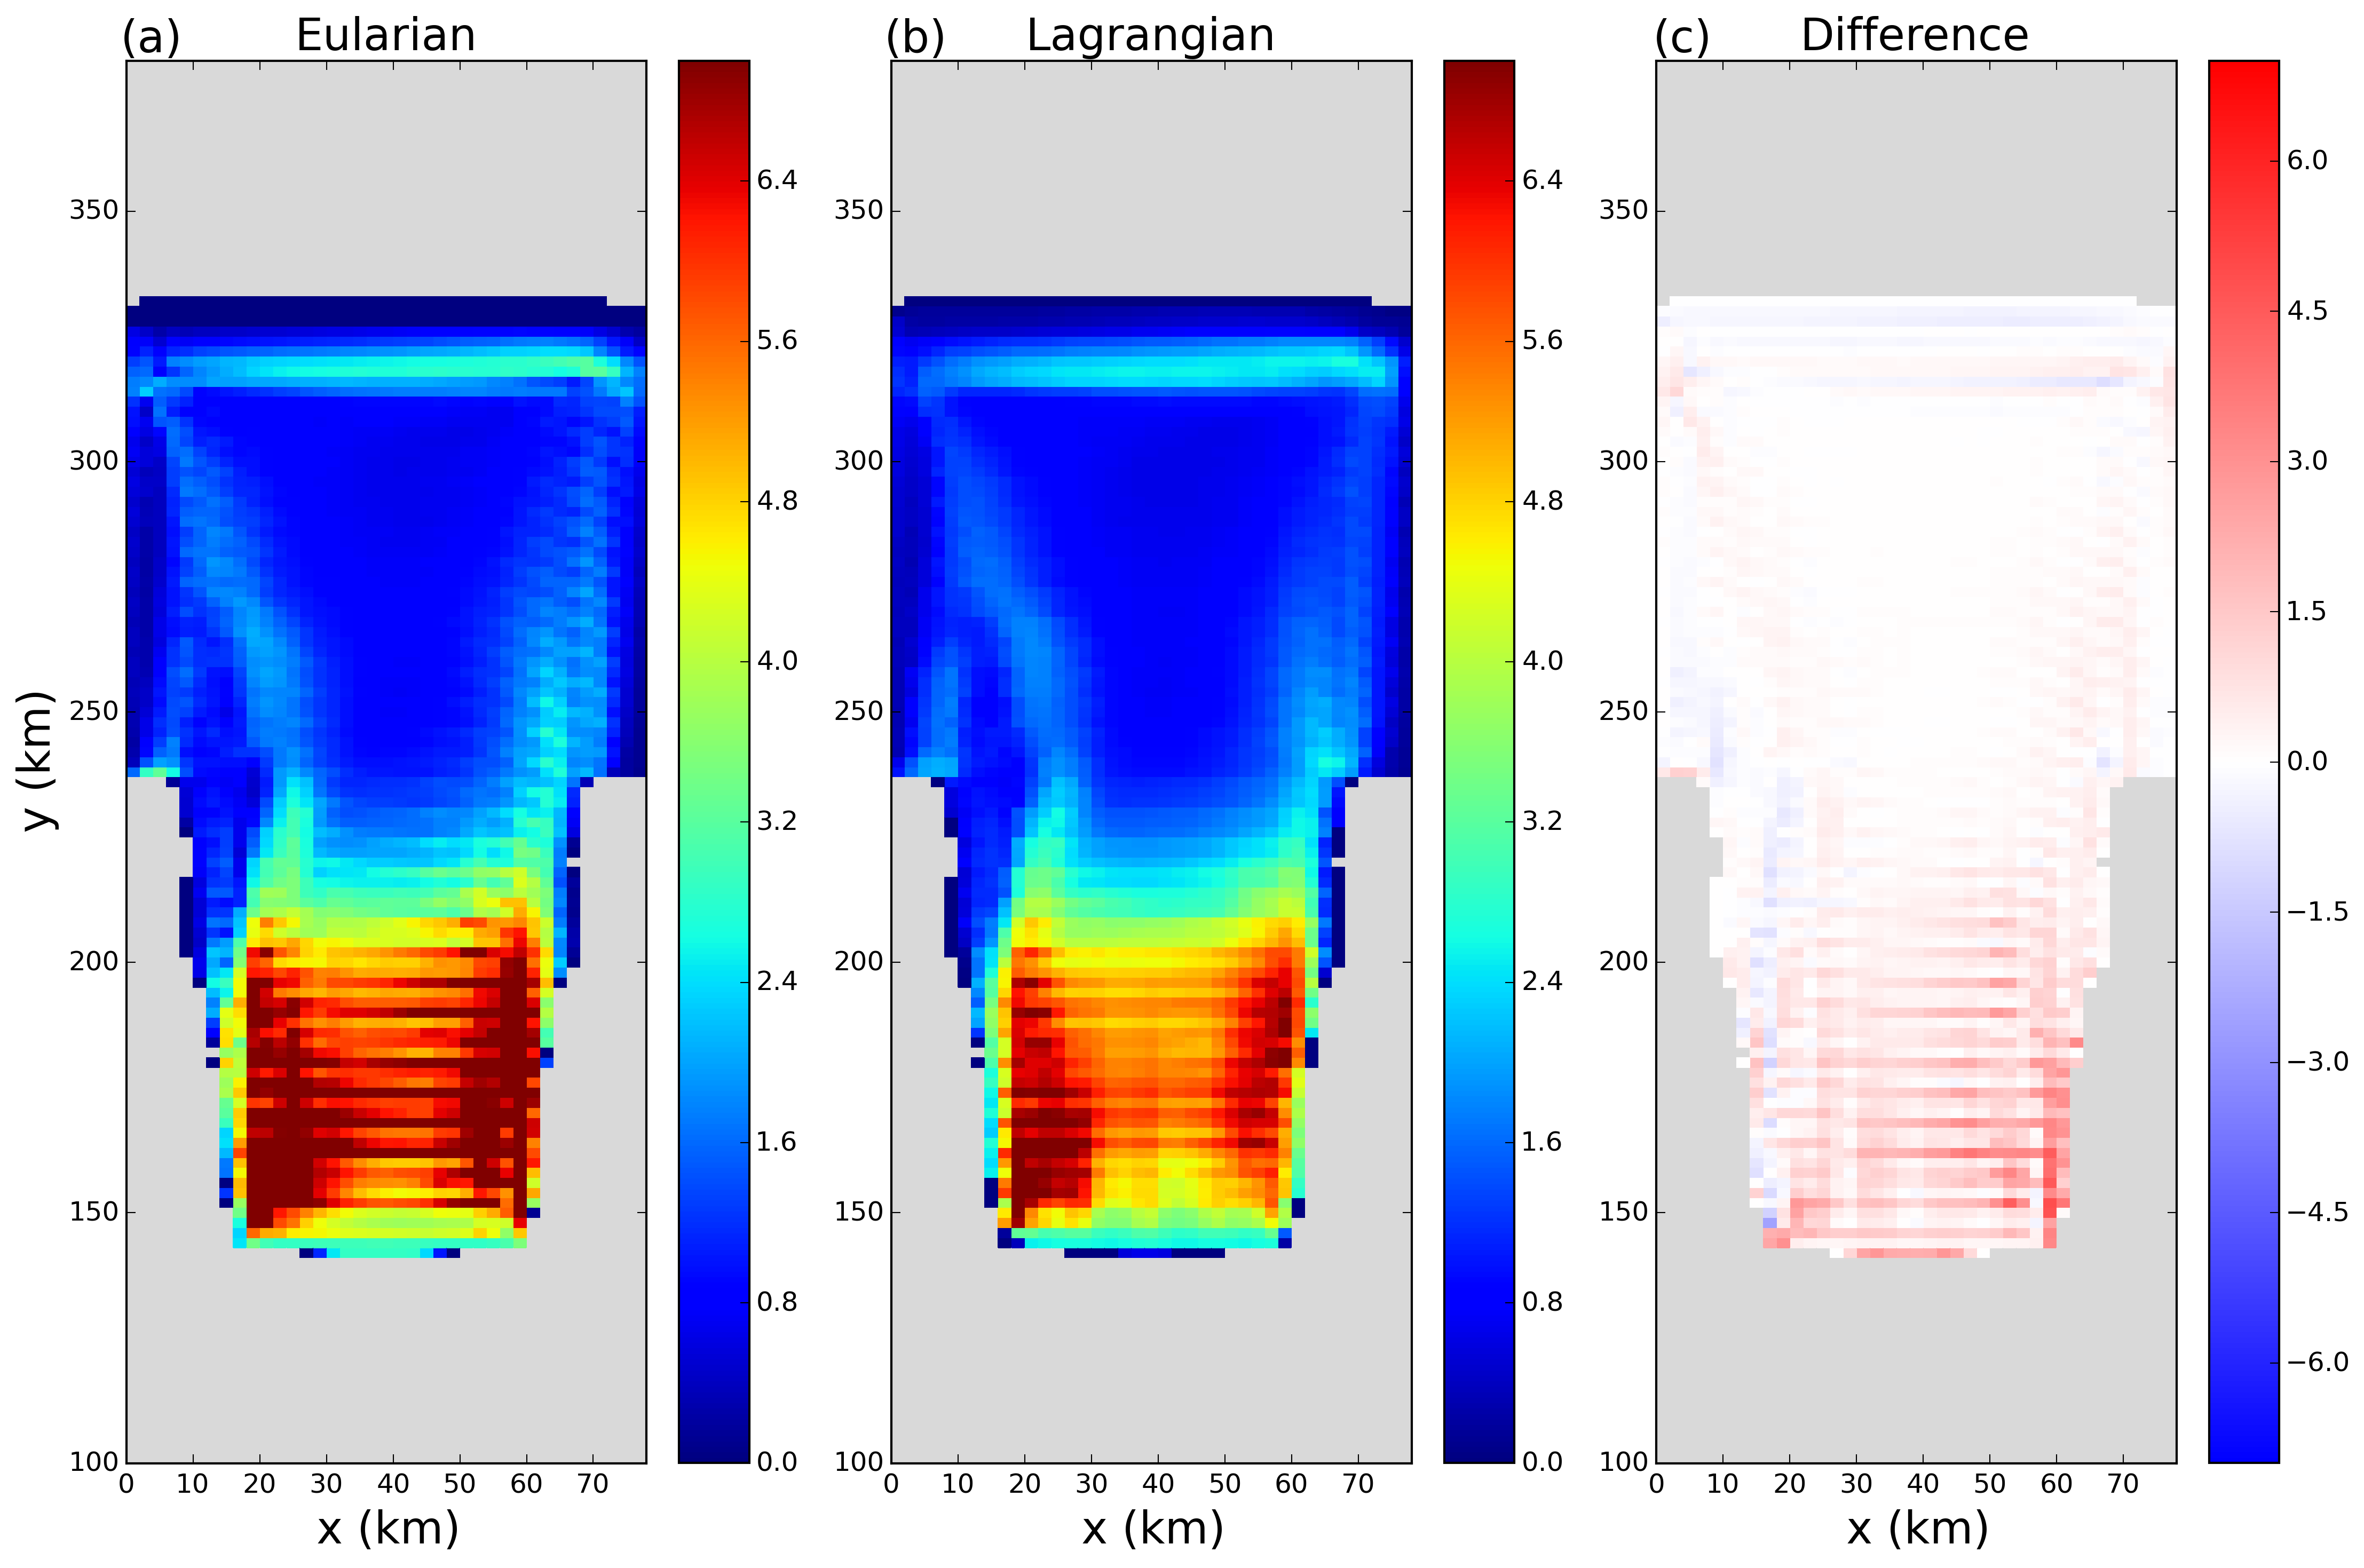
\includegraphics[width=0.99\textwidth]{Figures/ALE_z_static_shelf_comparison_melt.png}
\caption{ {Time-averaged melt rates in the (a) Lagrangian and (b) Eulerian simulations in the static ice-shelf configuration. Panel (c) shows the difference between panels (a) and (b). The time averages are taken over 5 years of model time, beginning at the end of the 5 year spin up period.}}
\end{center}
\label{fig:Melt_comparison}
\end{figure}
 \clearpage




\begin{figure}
\begin{center}
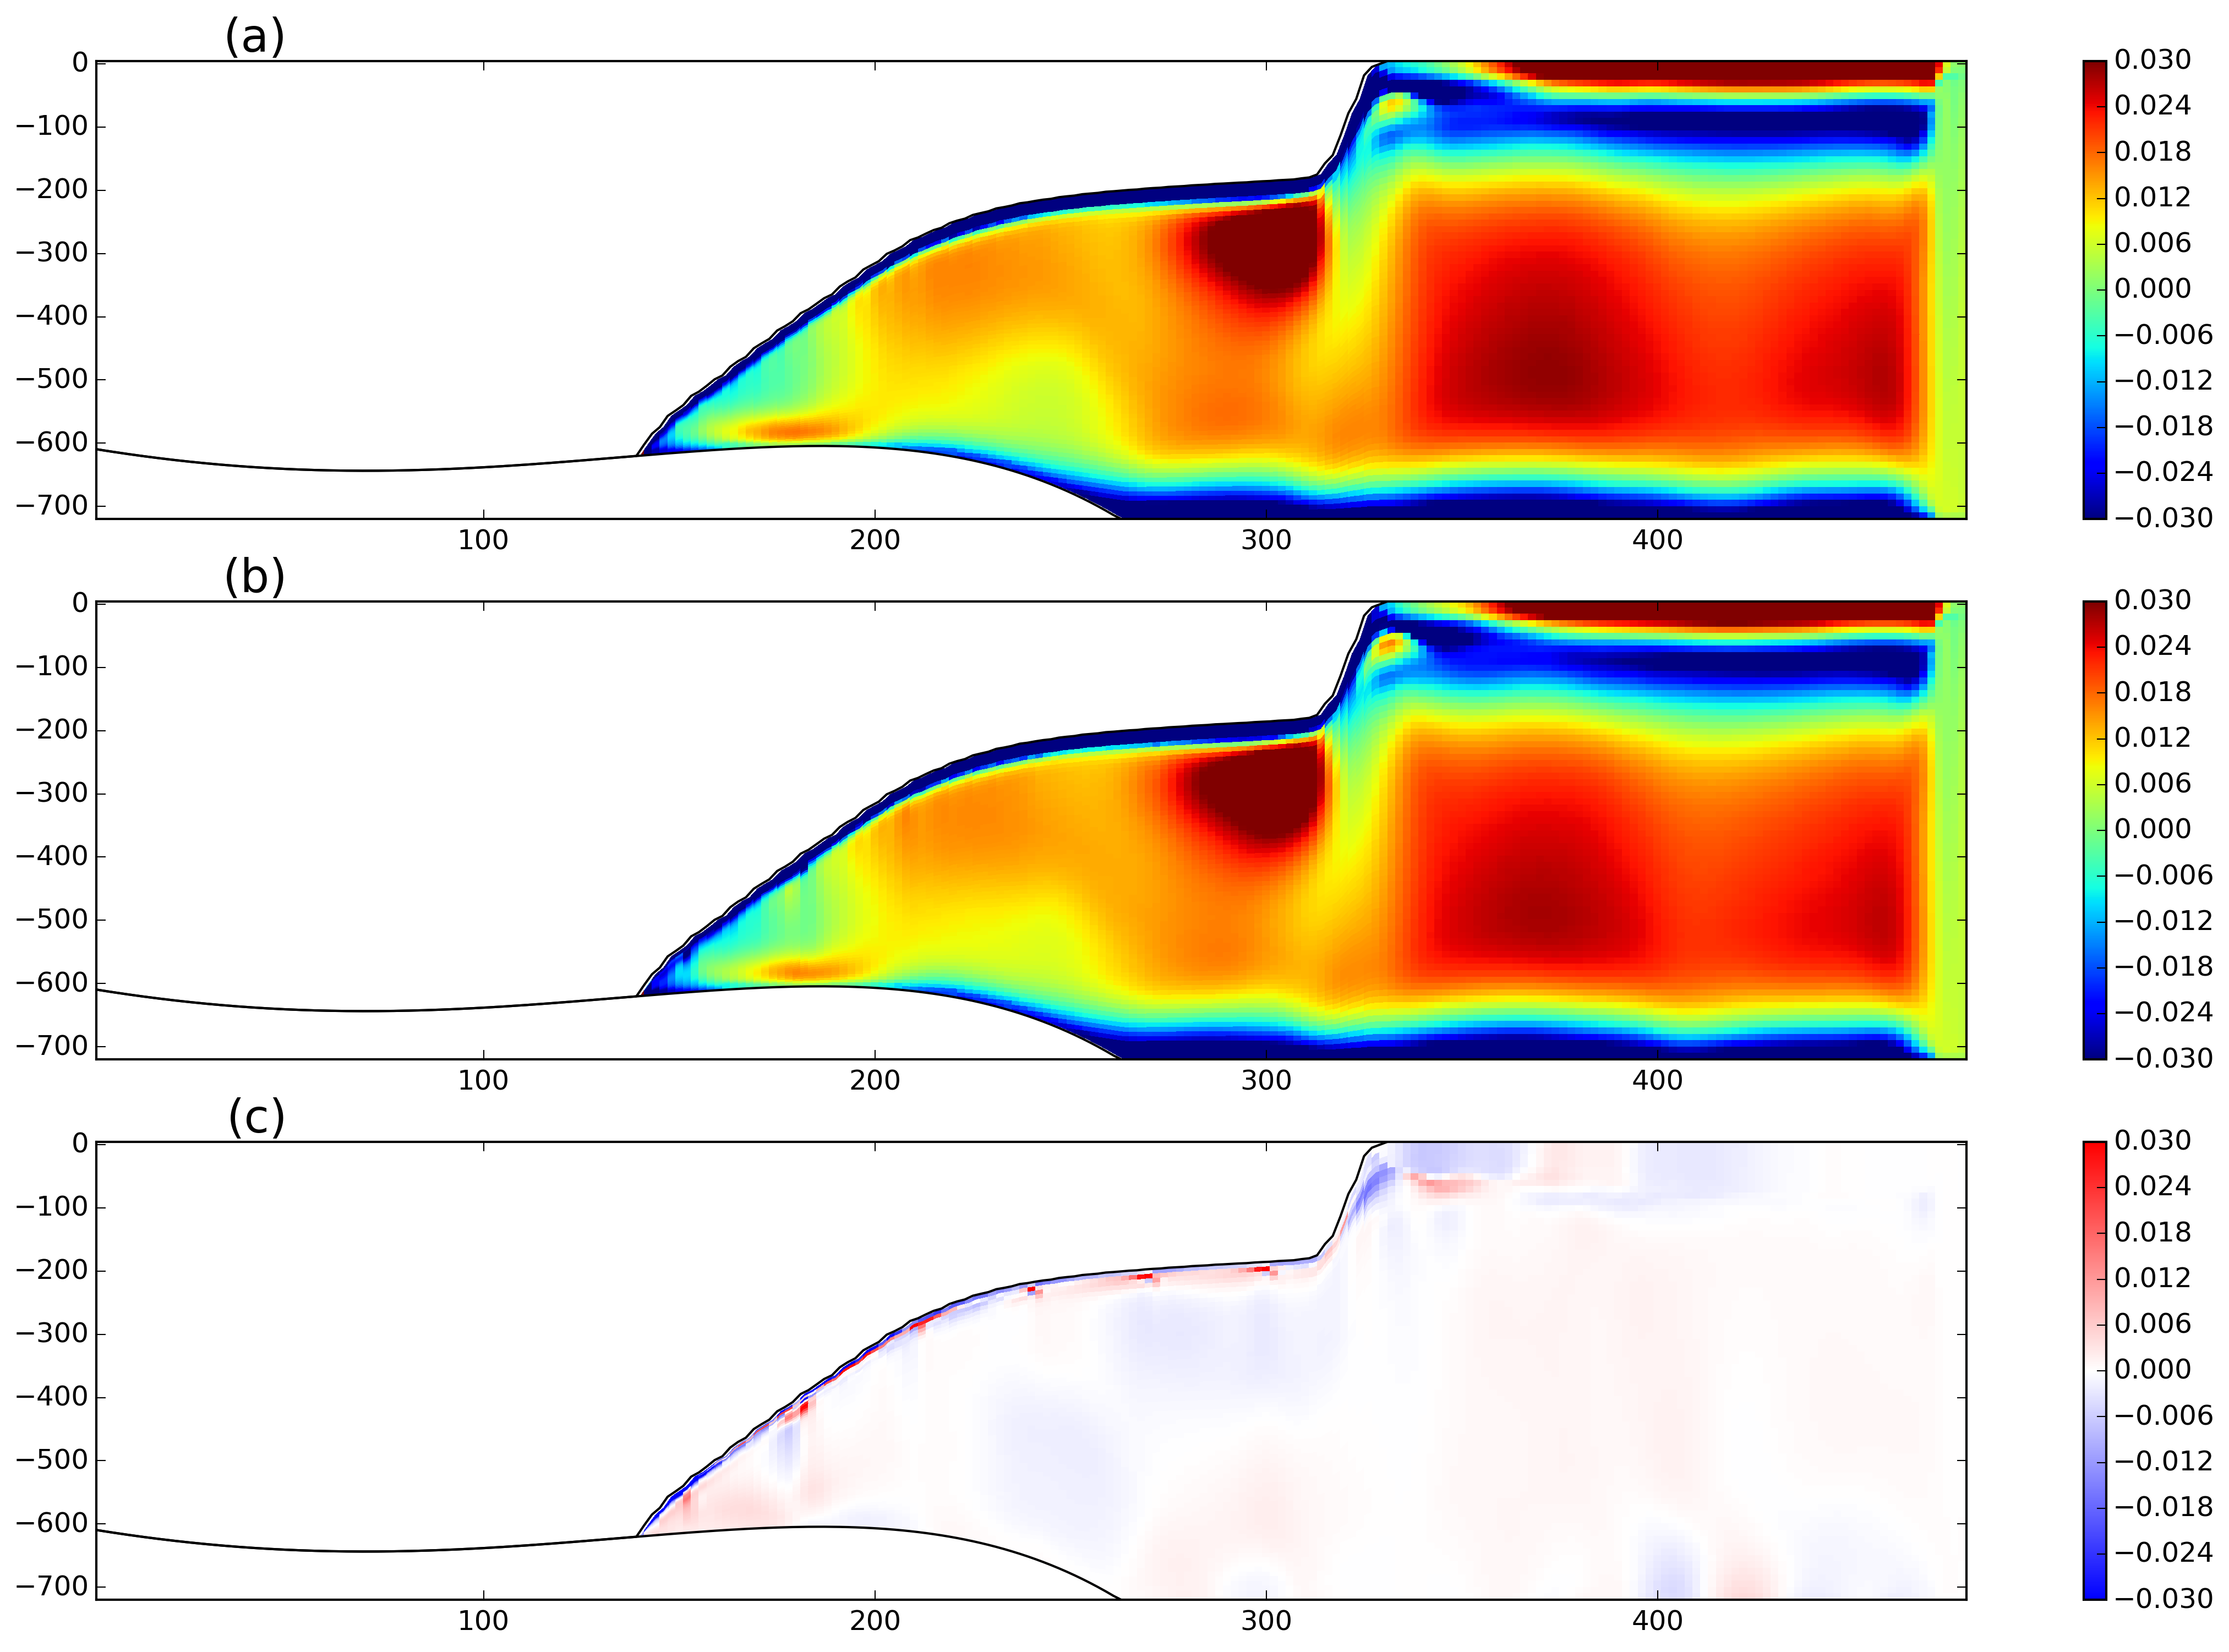
\includegraphics[width=0.99\textwidth]{Figures/Wind_static_shelf_comparison_salt_layers.png}
%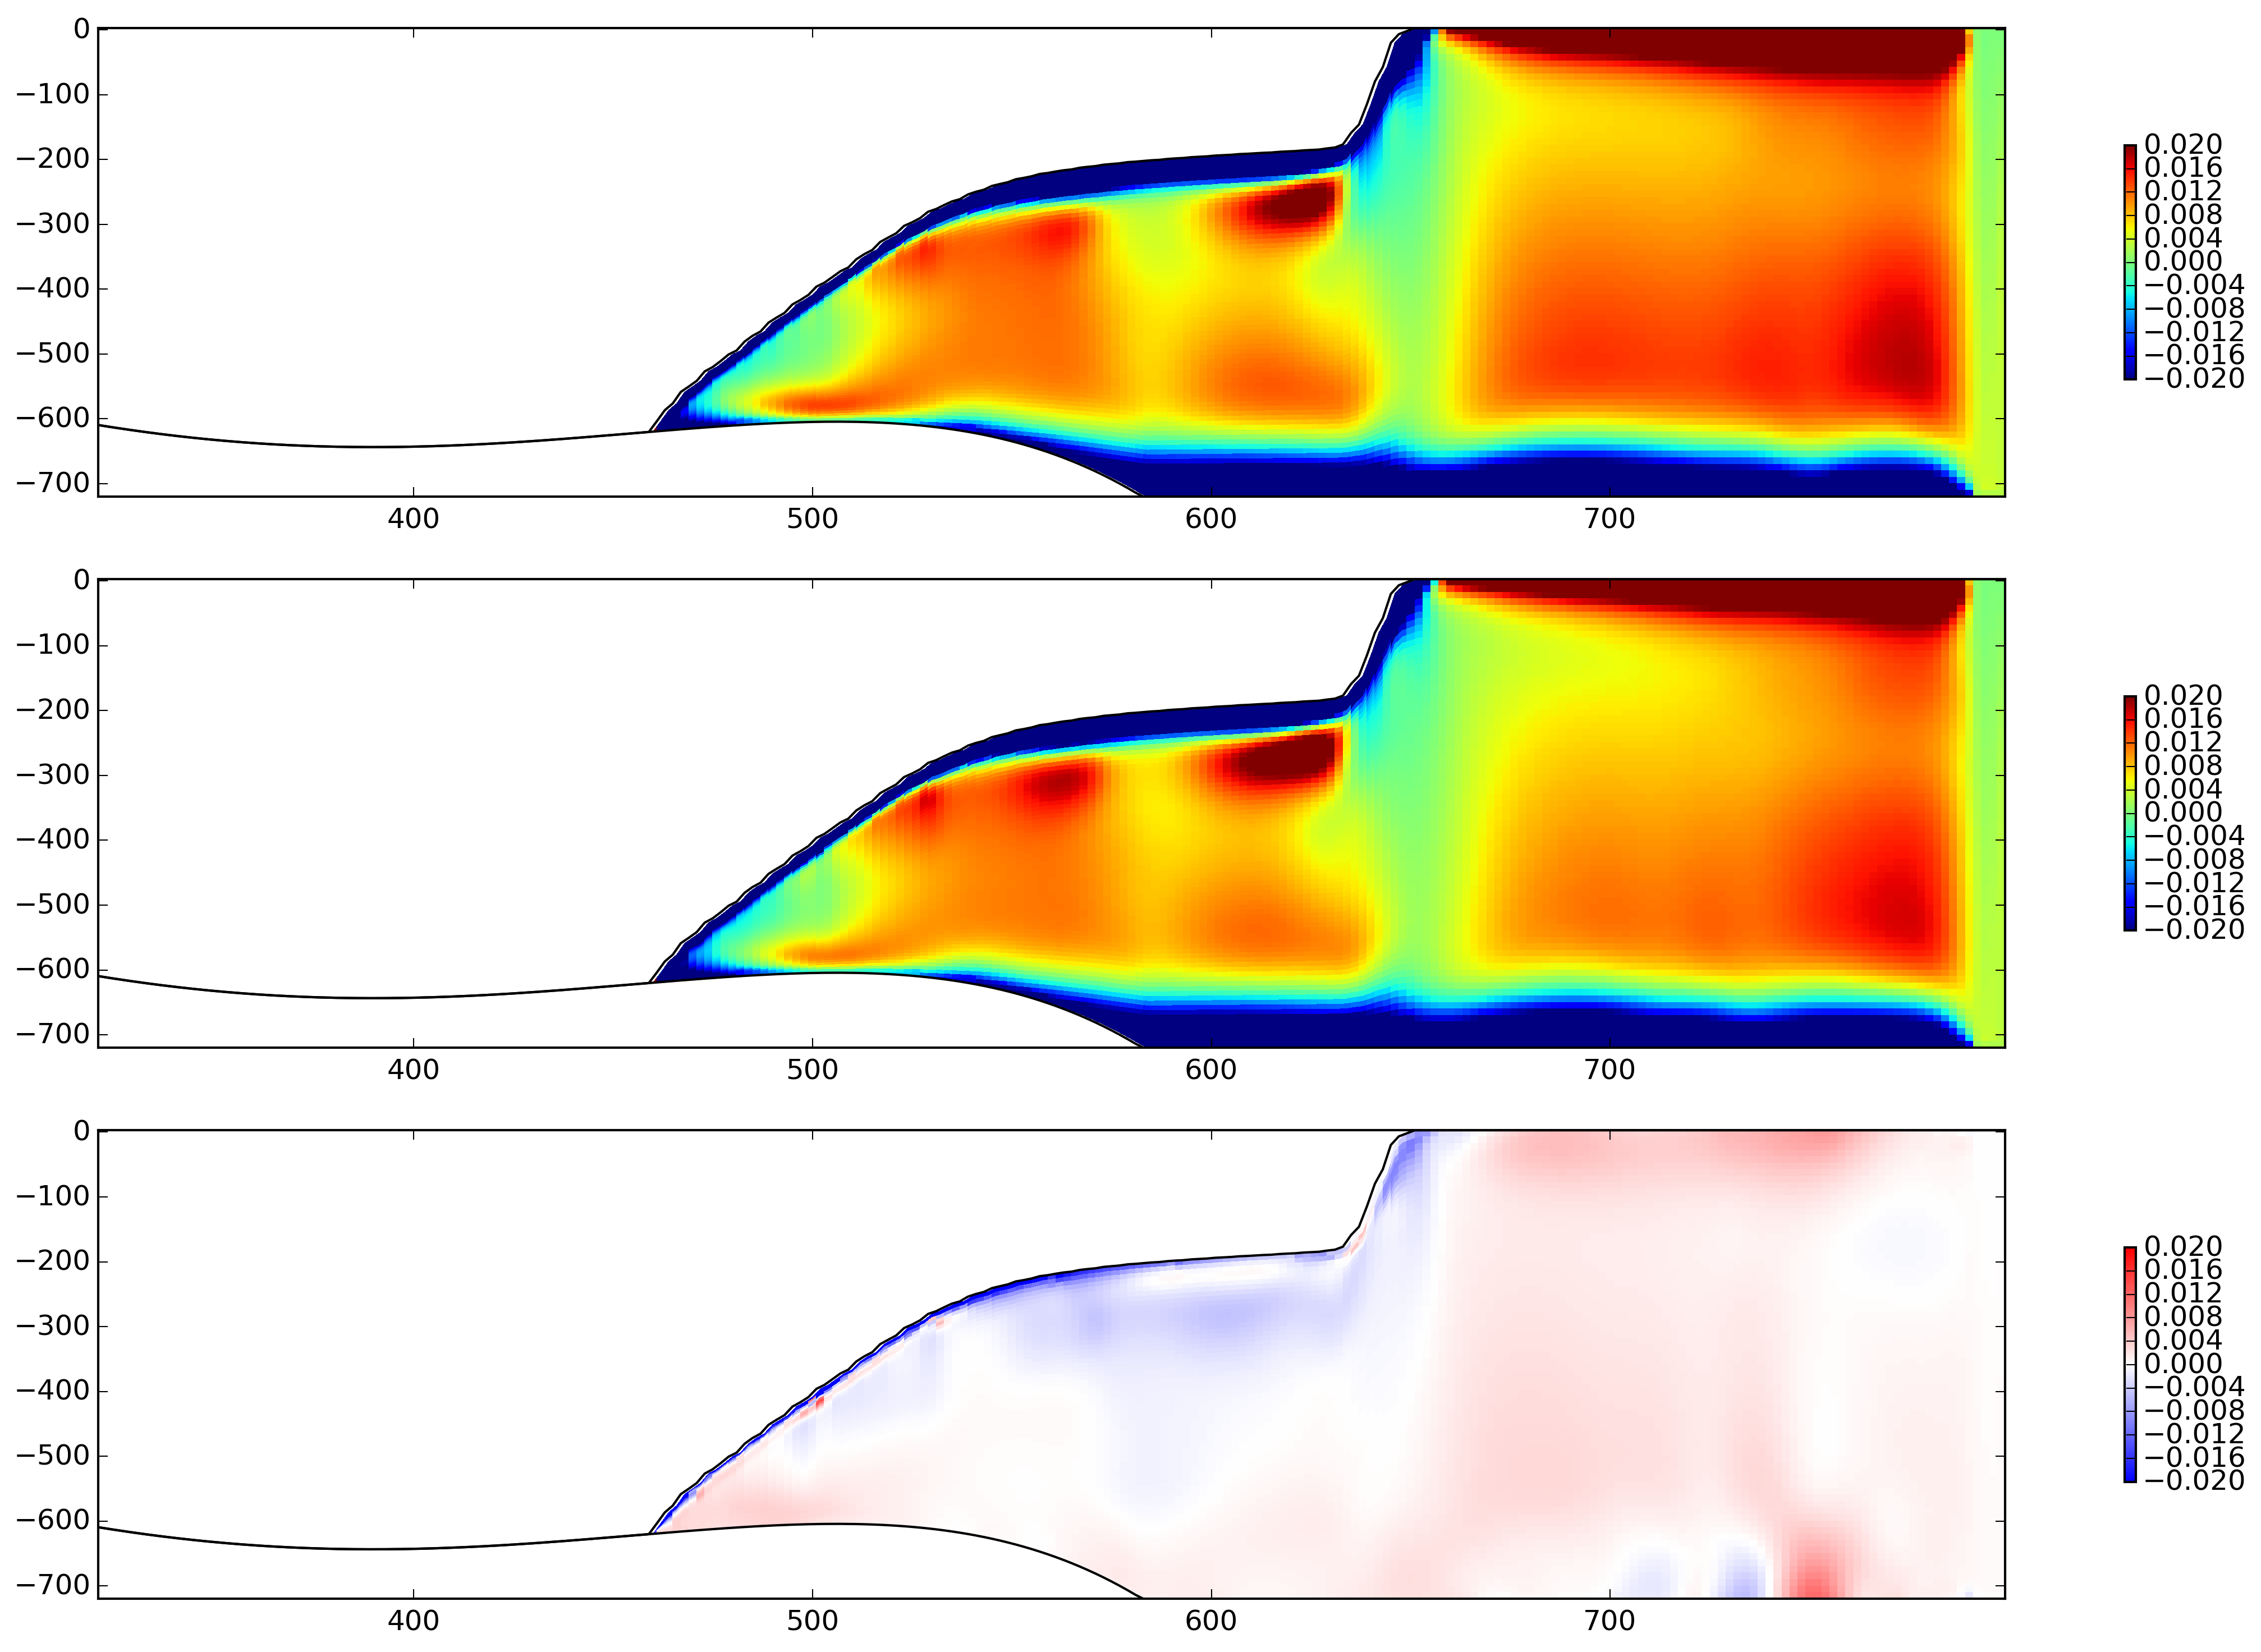
\includegraphics[width=0.99\textwidth]{Figures/ALE_z_static_shelf_comparison_salt_layers.png}
\caption{ {Time-averaged vertical sections of salinity at  $x$=40~km in the (a) Lagrangian and (b) Eulerian simulations in the static ice-shelf configuration. Panel (c) shows the difference between panels (a) and (b). The time averages are taken over 5 years of model time, beginning at the end of the 5 year spin up period. The position of the vertical transects is shown by the black dashed lines in Figure \ref{fig:SST_snapshots}a.
}}
\end{center}
\label{fig:Salt_comparison}
\end{figure}
 \clearpage

  
 \begin{figure}
\begin{center}
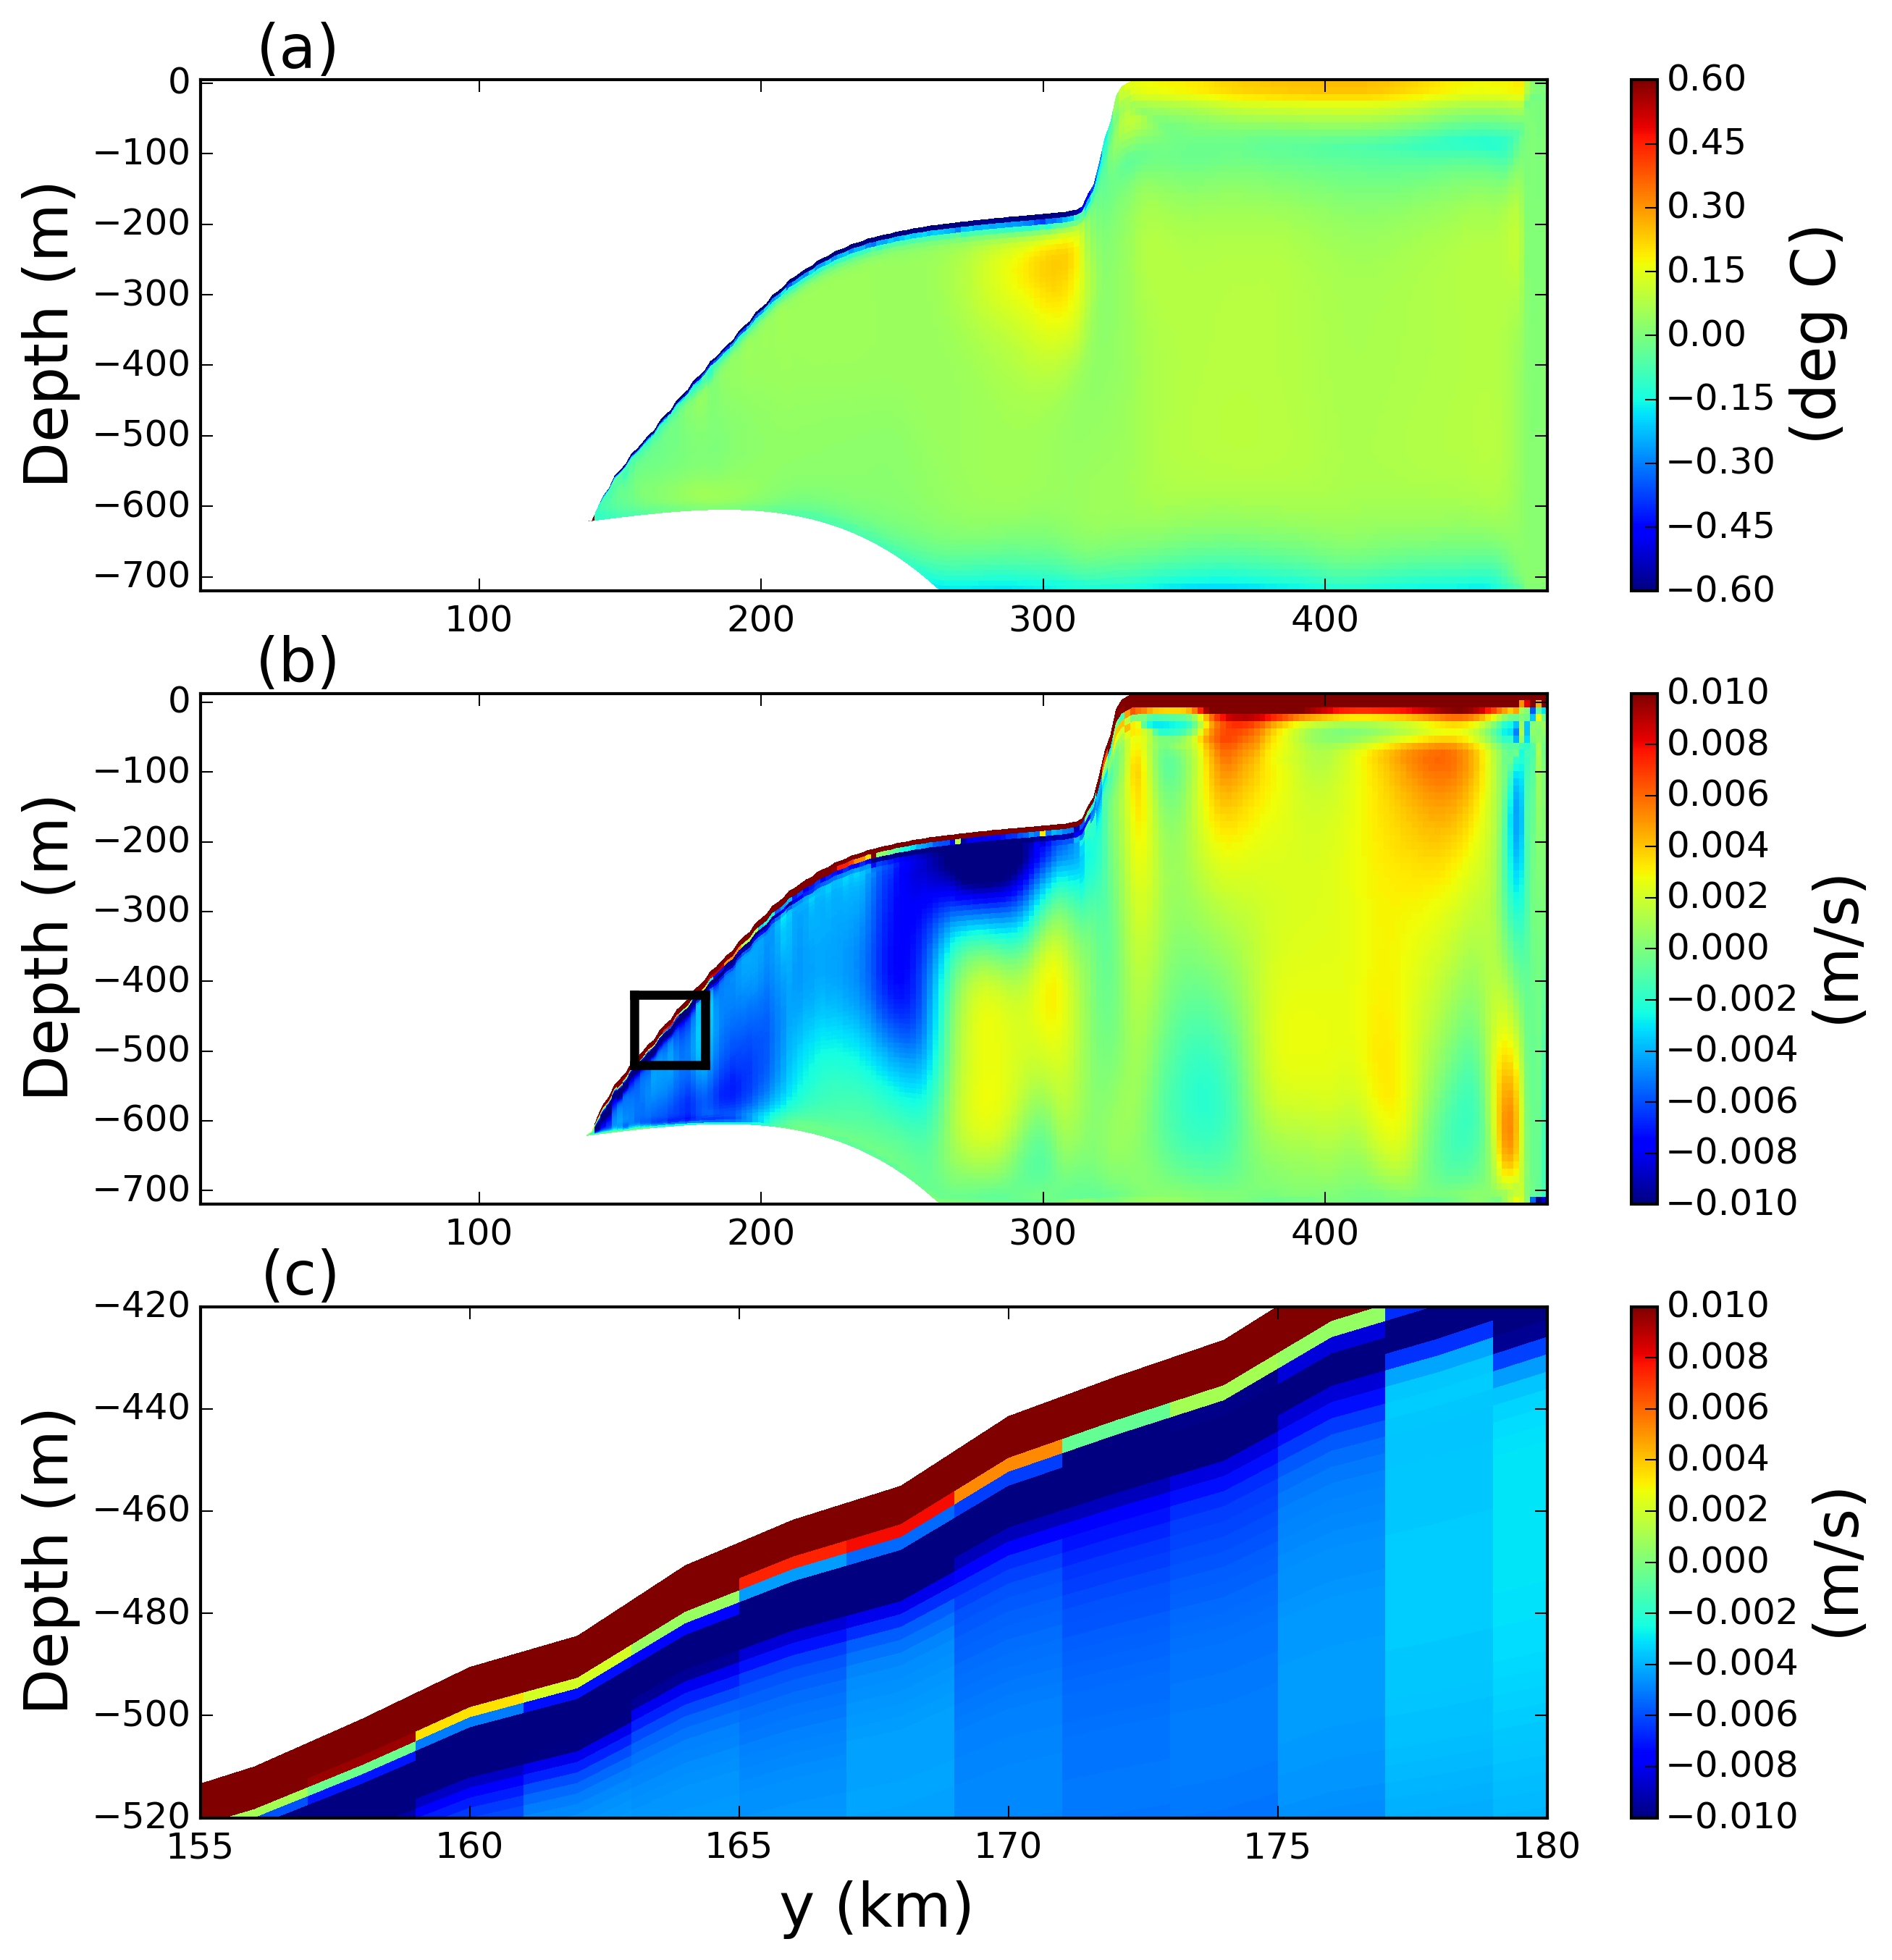
\includegraphics[width=0.99\textwidth]{Figures/Wind_static_shelf_solo_temp_v_v.png}
%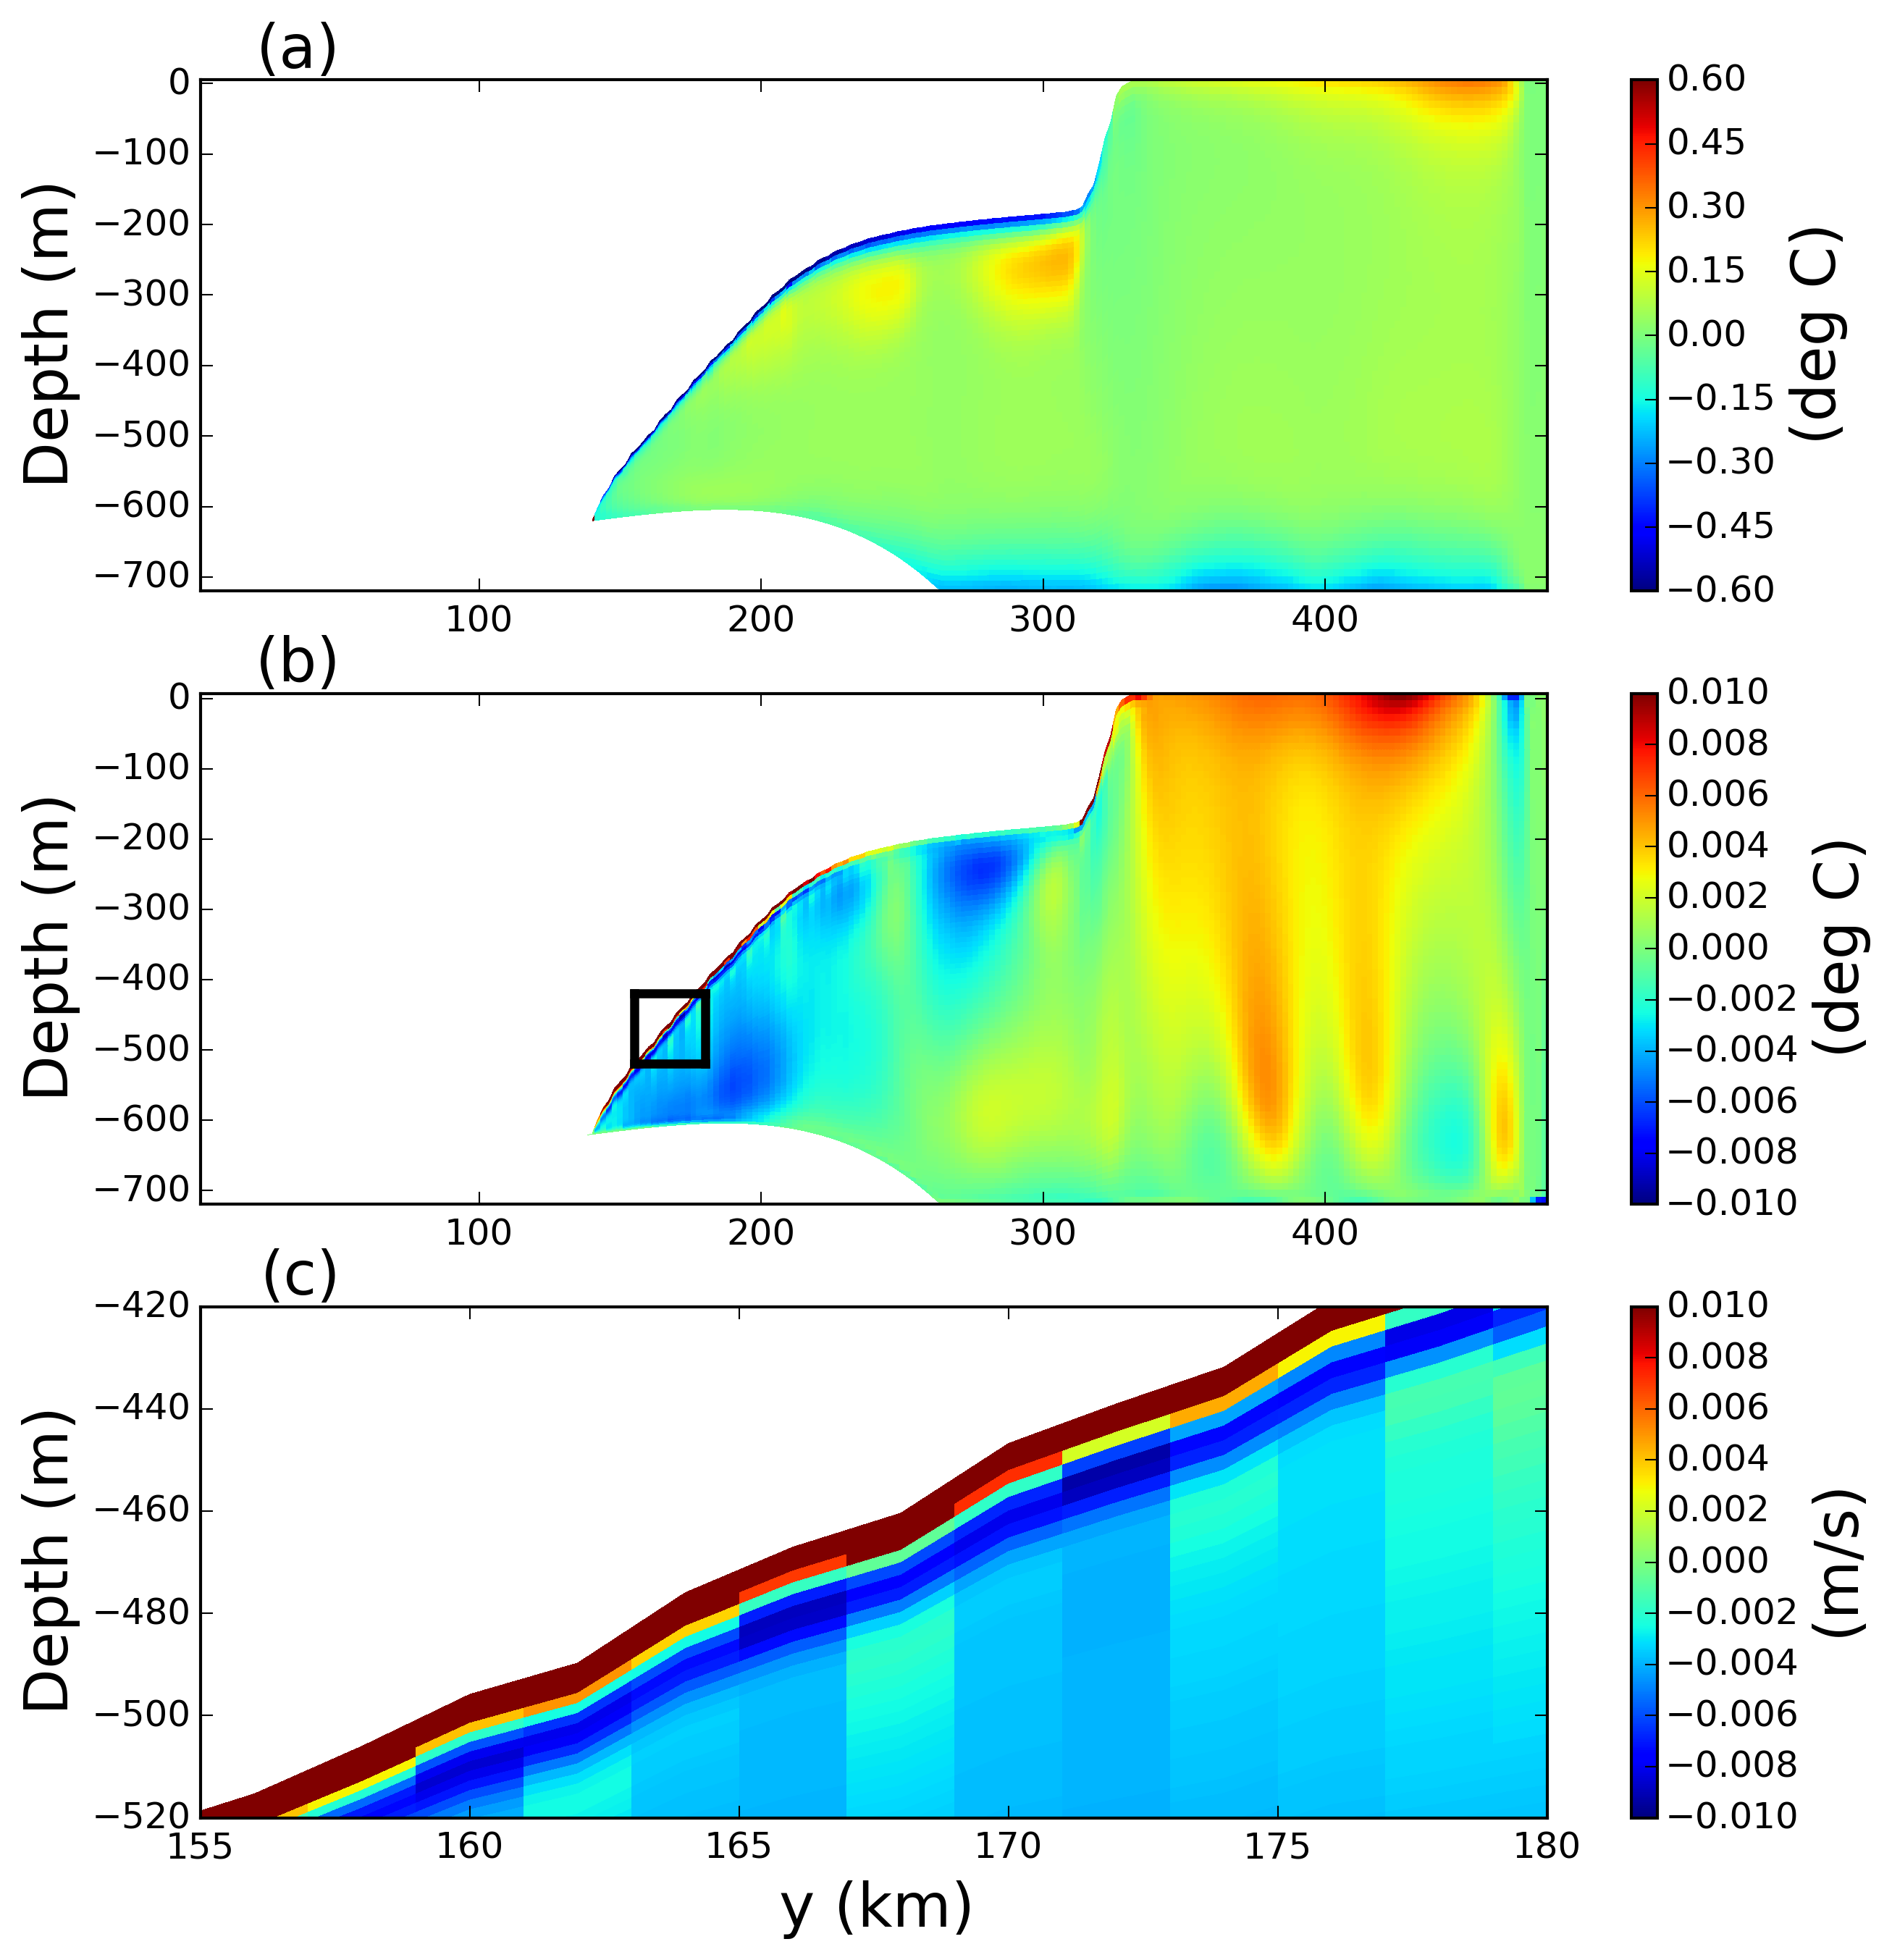
\includegraphics[width=0.99\textwidth]{Figures/ALE_z_static_shelf_solo_temp_v_v.png}
\caption{ {Snapshots of the static ice-shelf experiment taken after 5 years of model simulation, using the Lagrangian ice-shelf model coupled to the MOM6 ocean model. Panels show cross sections of the (a) the steady-state ocean temperature, and (b) the meridional ocean velocity. Panel (c) again shows the meridional ocean velocity, and is zoomed into the region near the ice-shelf base (the zoomed-in region is indicated with a black box (b)).}}
\end{center}
\label{fig:static_solo_temp_v_v}
\end{figure} 
 \clearpage

 


 
\begin{figure}
\begin{center}
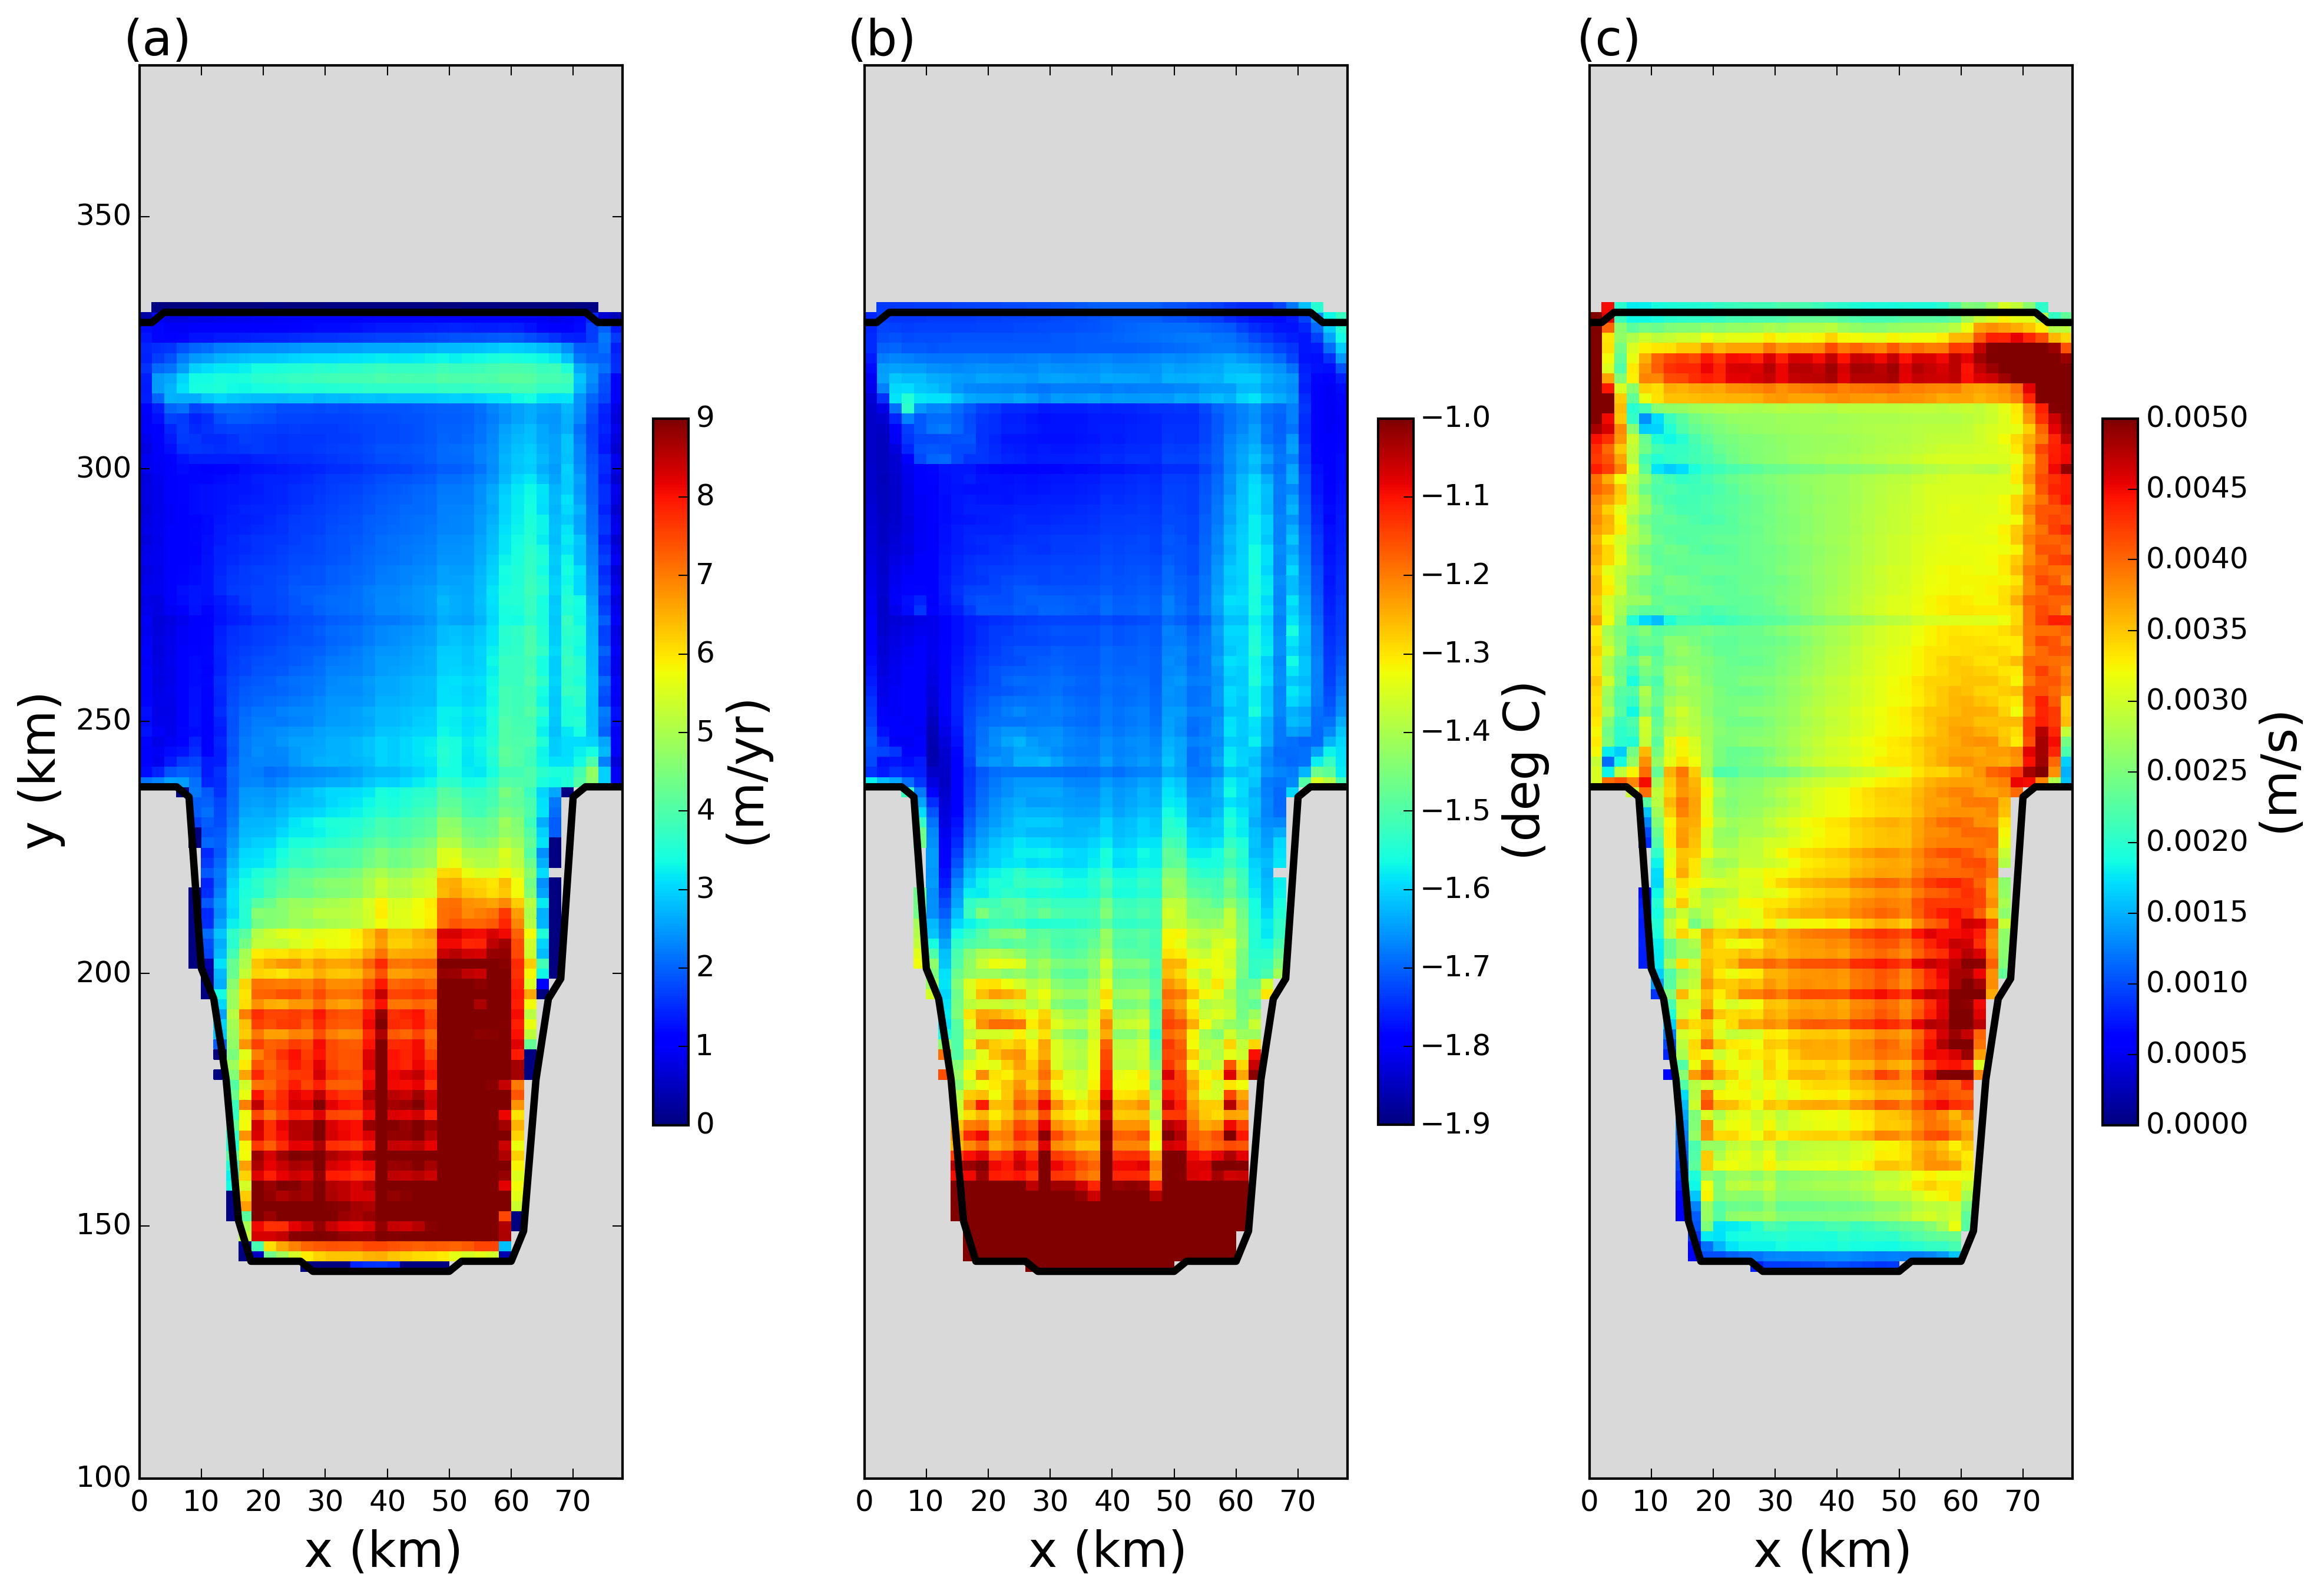
\includegraphics[width=0.99\textwidth]{Figures/Wind_static_shelf_solo_melt_m_per_year_sst_ustar_iceberg.png}
%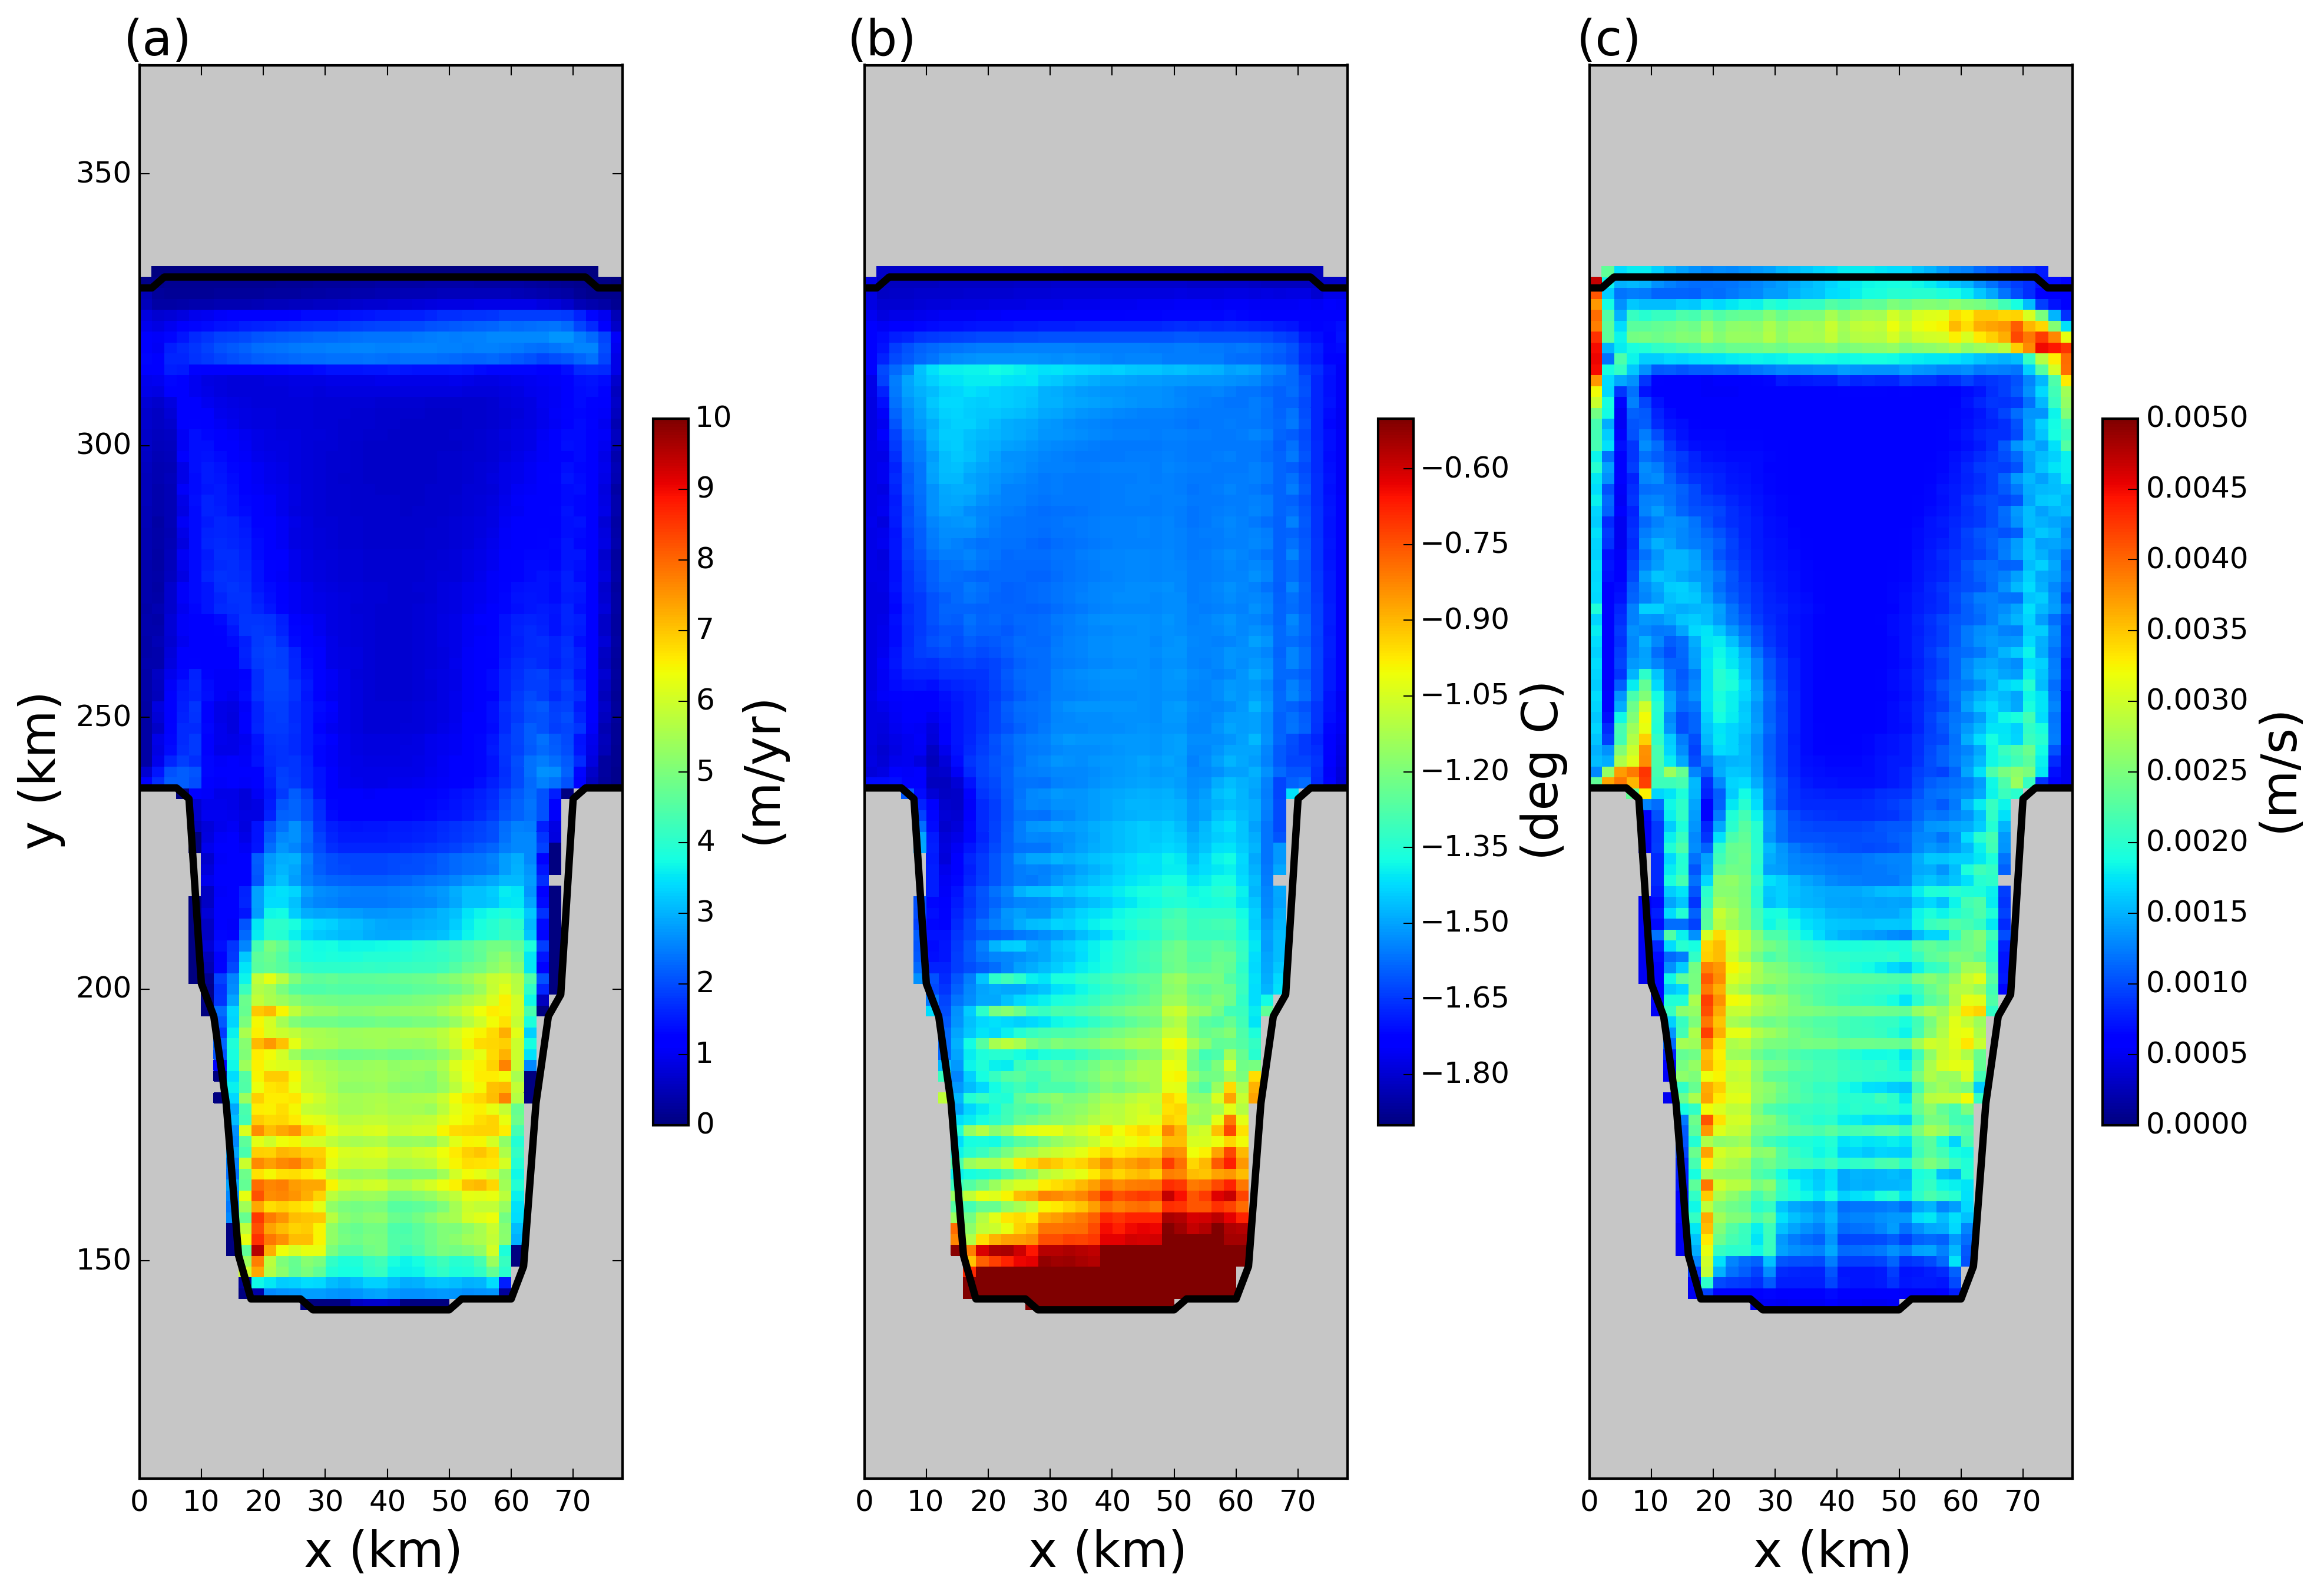
\includegraphics[width=0.99\textwidth]{Figures/ALE_z_static_shelf_solo_melt_m_per_year_sst_ustar_iceberg.png}
\caption{ {Results of the static ice-shelf experiment using the Lagrangian ice-shelf model coupled to MOM6. The three panels show 5 year time average of the (a) melt rate, (b) top-of-ocean temperature and (c) frictional velocity, $u^{*}$, at the base of the ice shelf. Fields are only shown in regions where the ice area fraction is $\geq 0.8$.}}
\end{center}
\label{fig:static_solo_melt}
\end{figure} 
 \clearpage


  
  \begin{figure}
\begin{center}
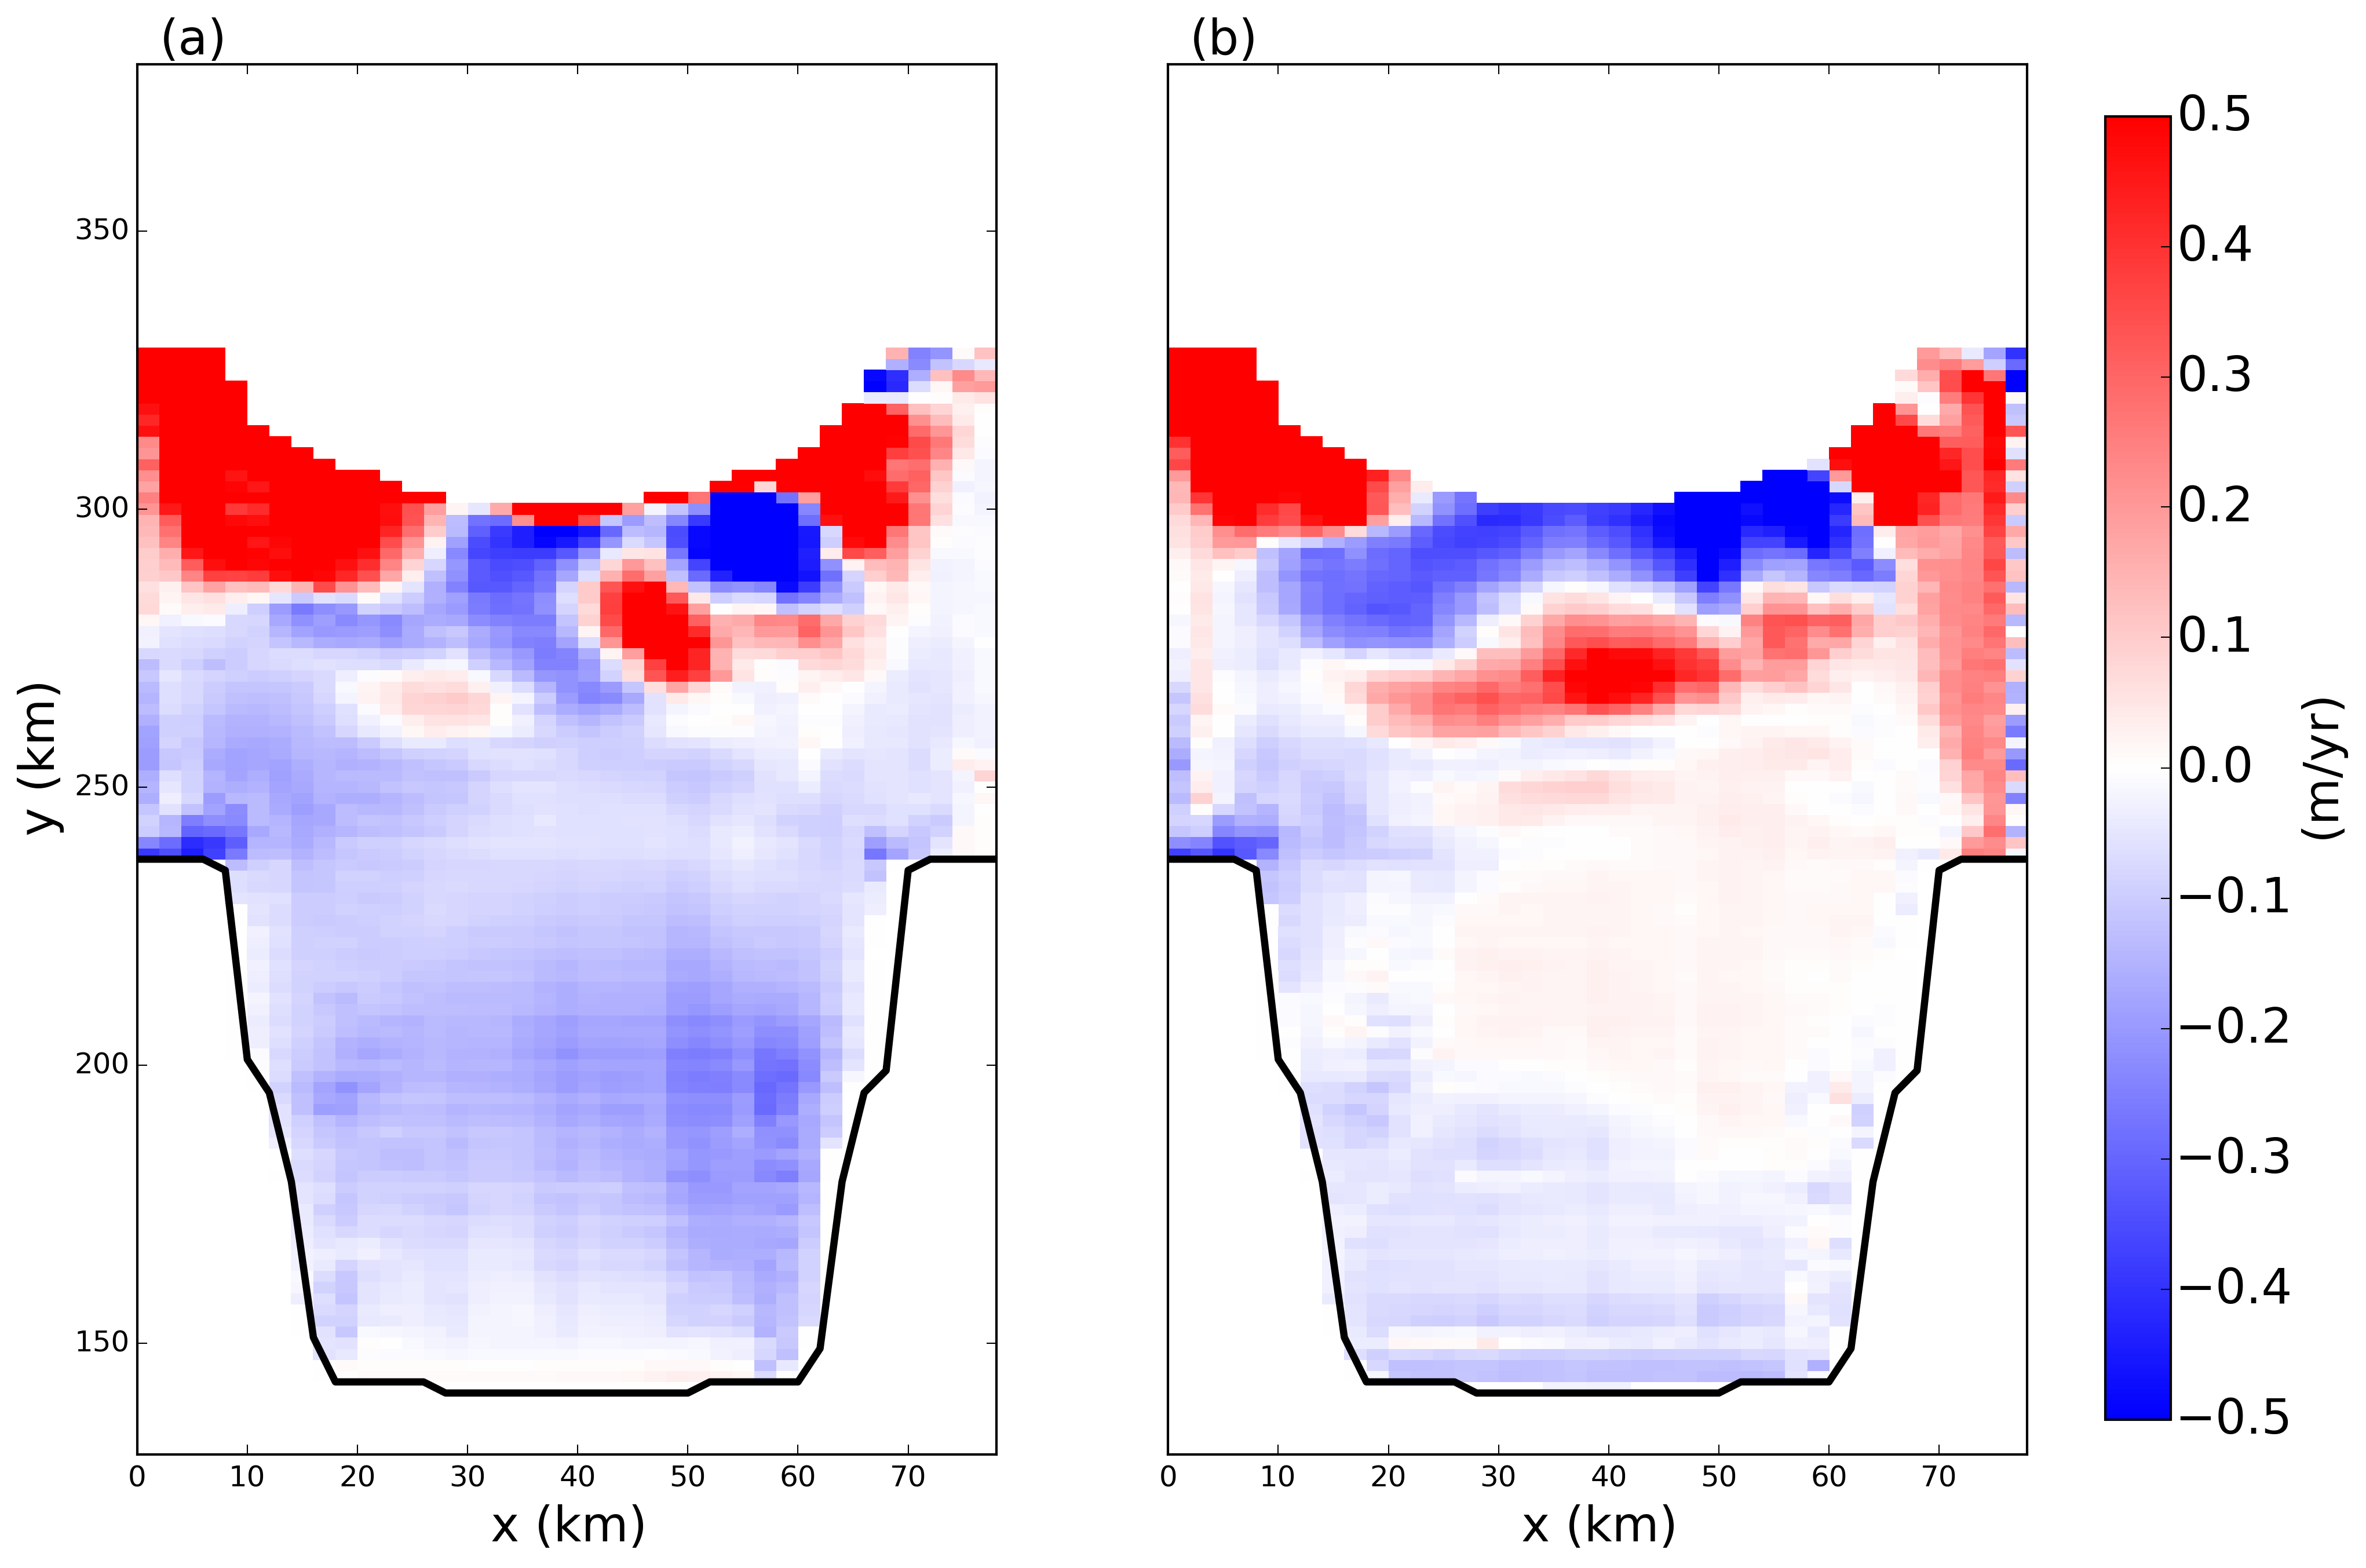
\includegraphics[width=0.99\textwidth]{Figures/snapshots_Wind_Wind_Broken_Compare_melt_m_per_year_anomaly.png}
%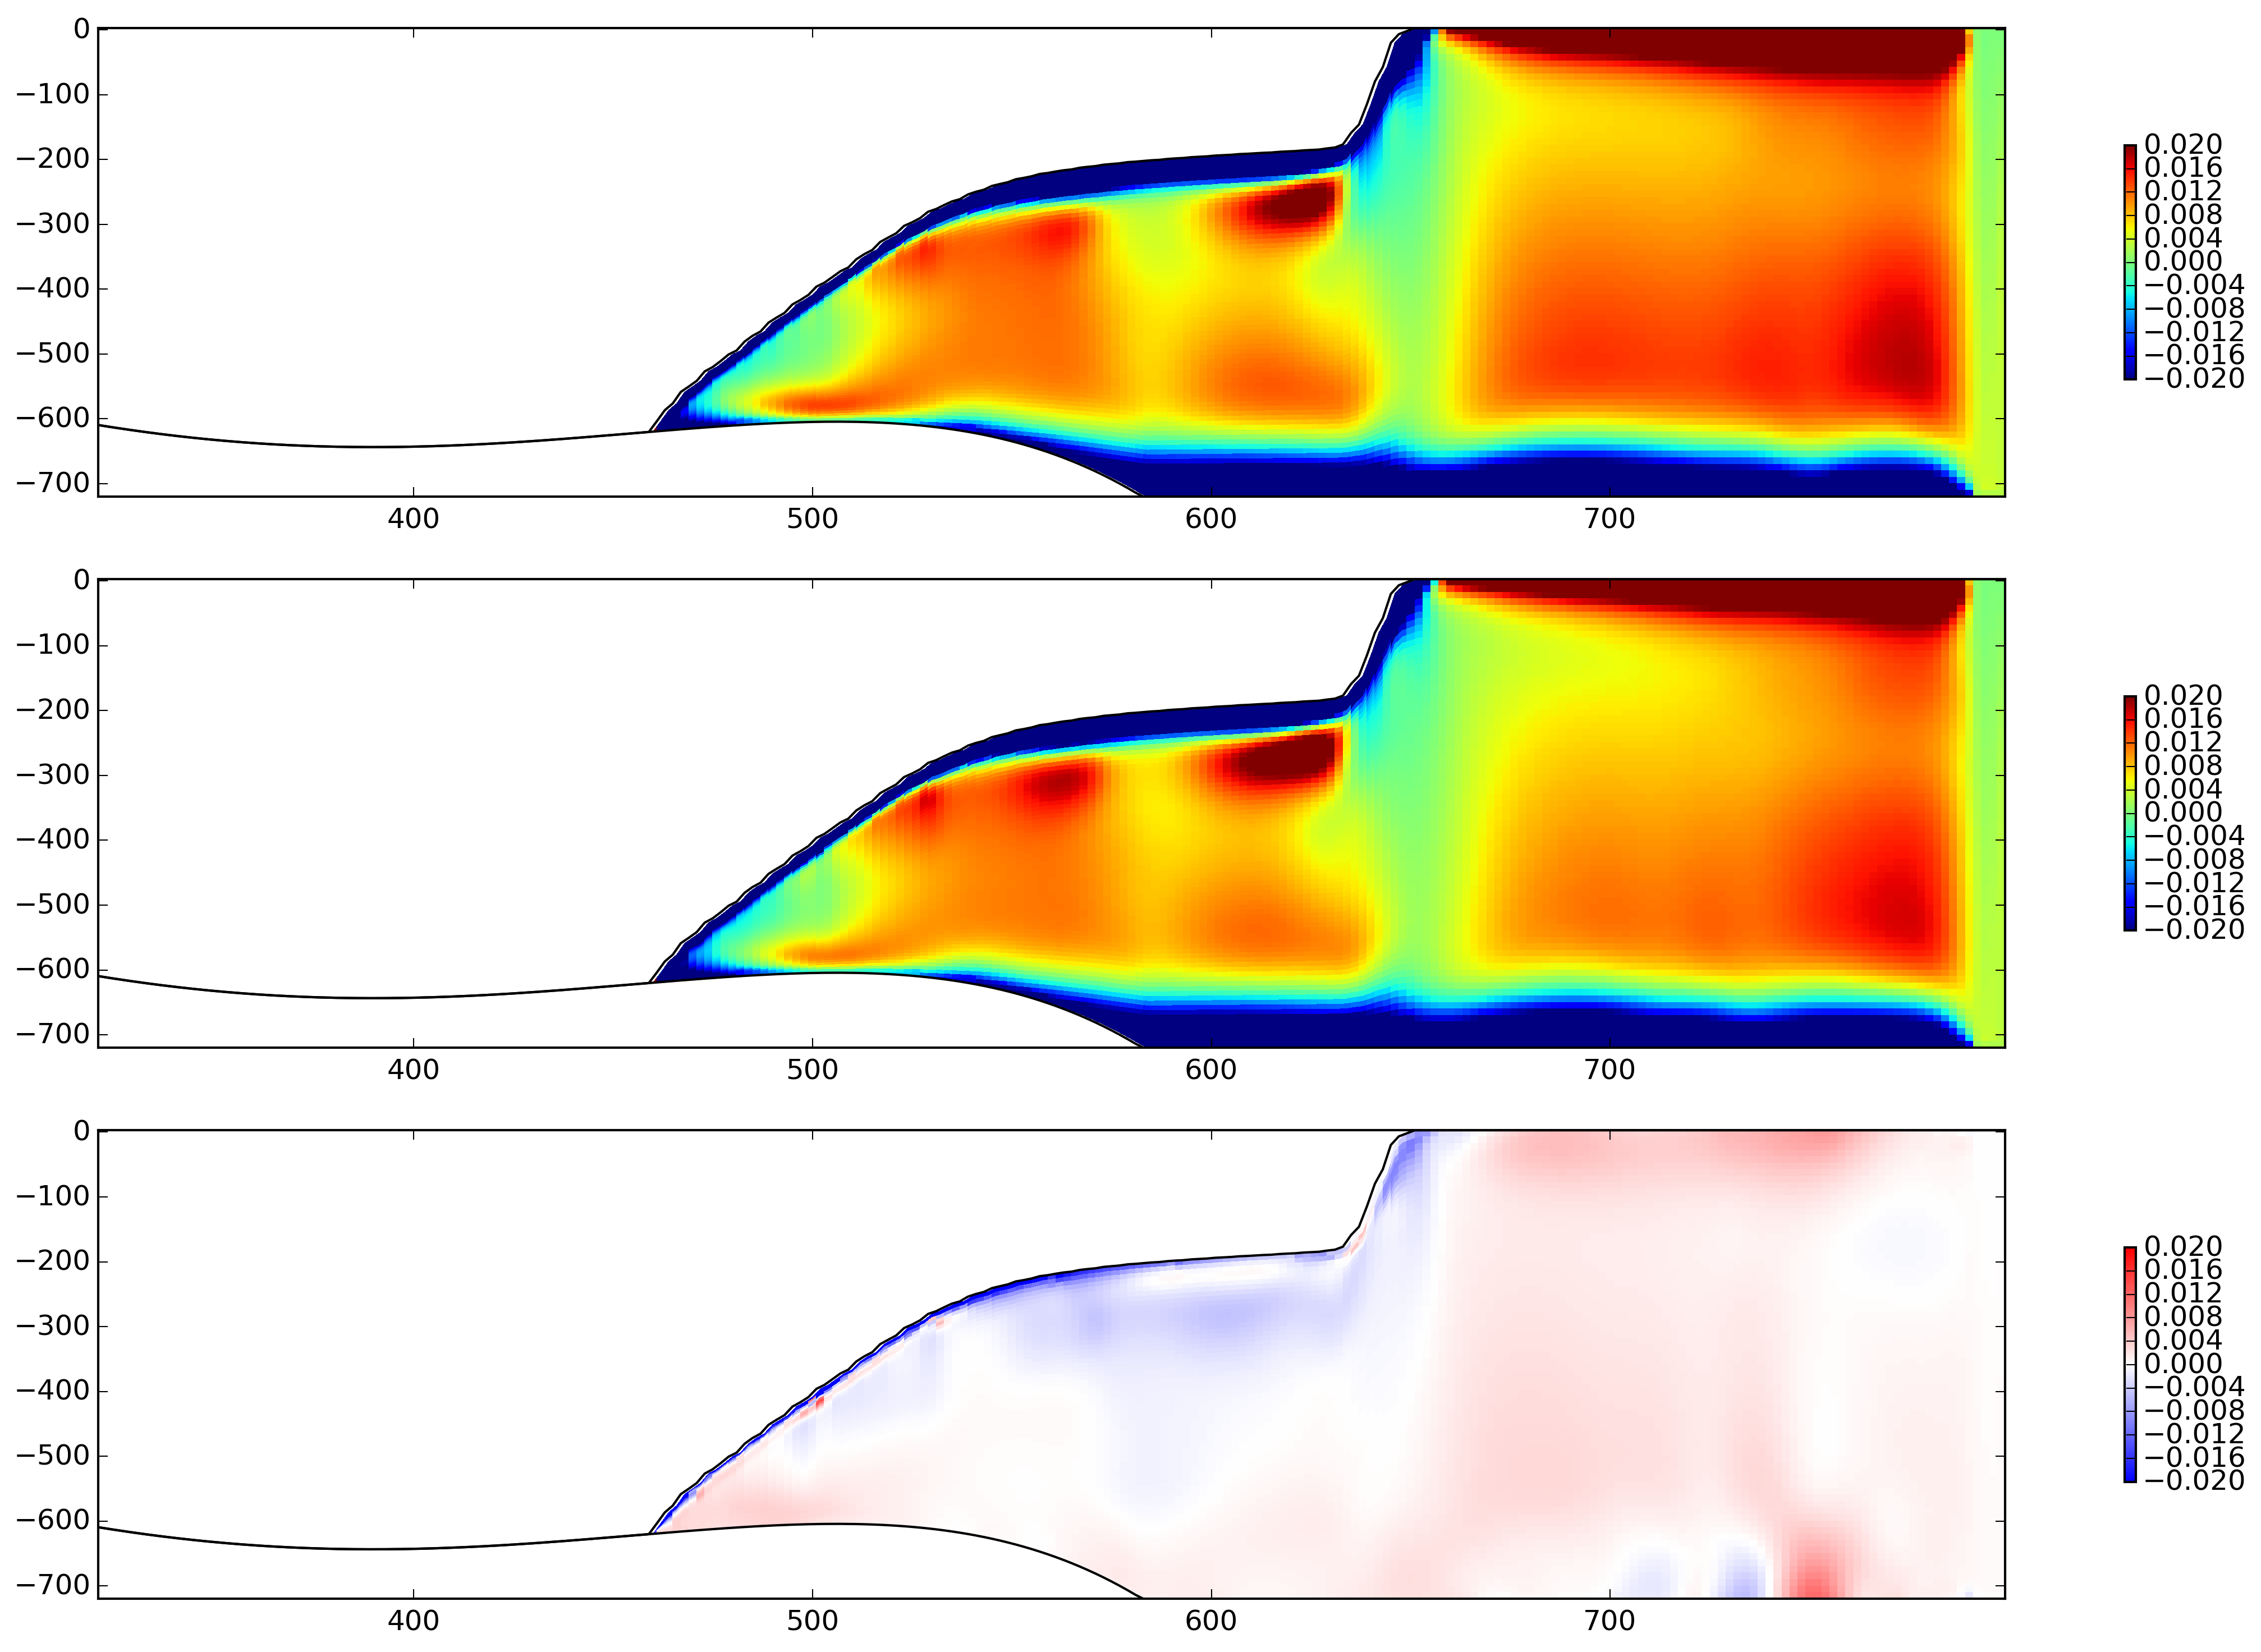
\includegraphics[width=0.99\textwidth]{Figures/ALE_z_static_shelf_comparison_salt_layers.png}
\caption{ {(a) Snapshot of the melt rate at the base of the ice shelf 60 days after the calving event in the tabular-iceberg-calving simulation. (b) Steady state melt rate of the simulation that was spun-up from rest with the semi-circular iceberg removed..}}
\end{center}
\label{fig:broken_melt}
\end{figure}
 \clearpage



\begin{figure}
\begin{center}
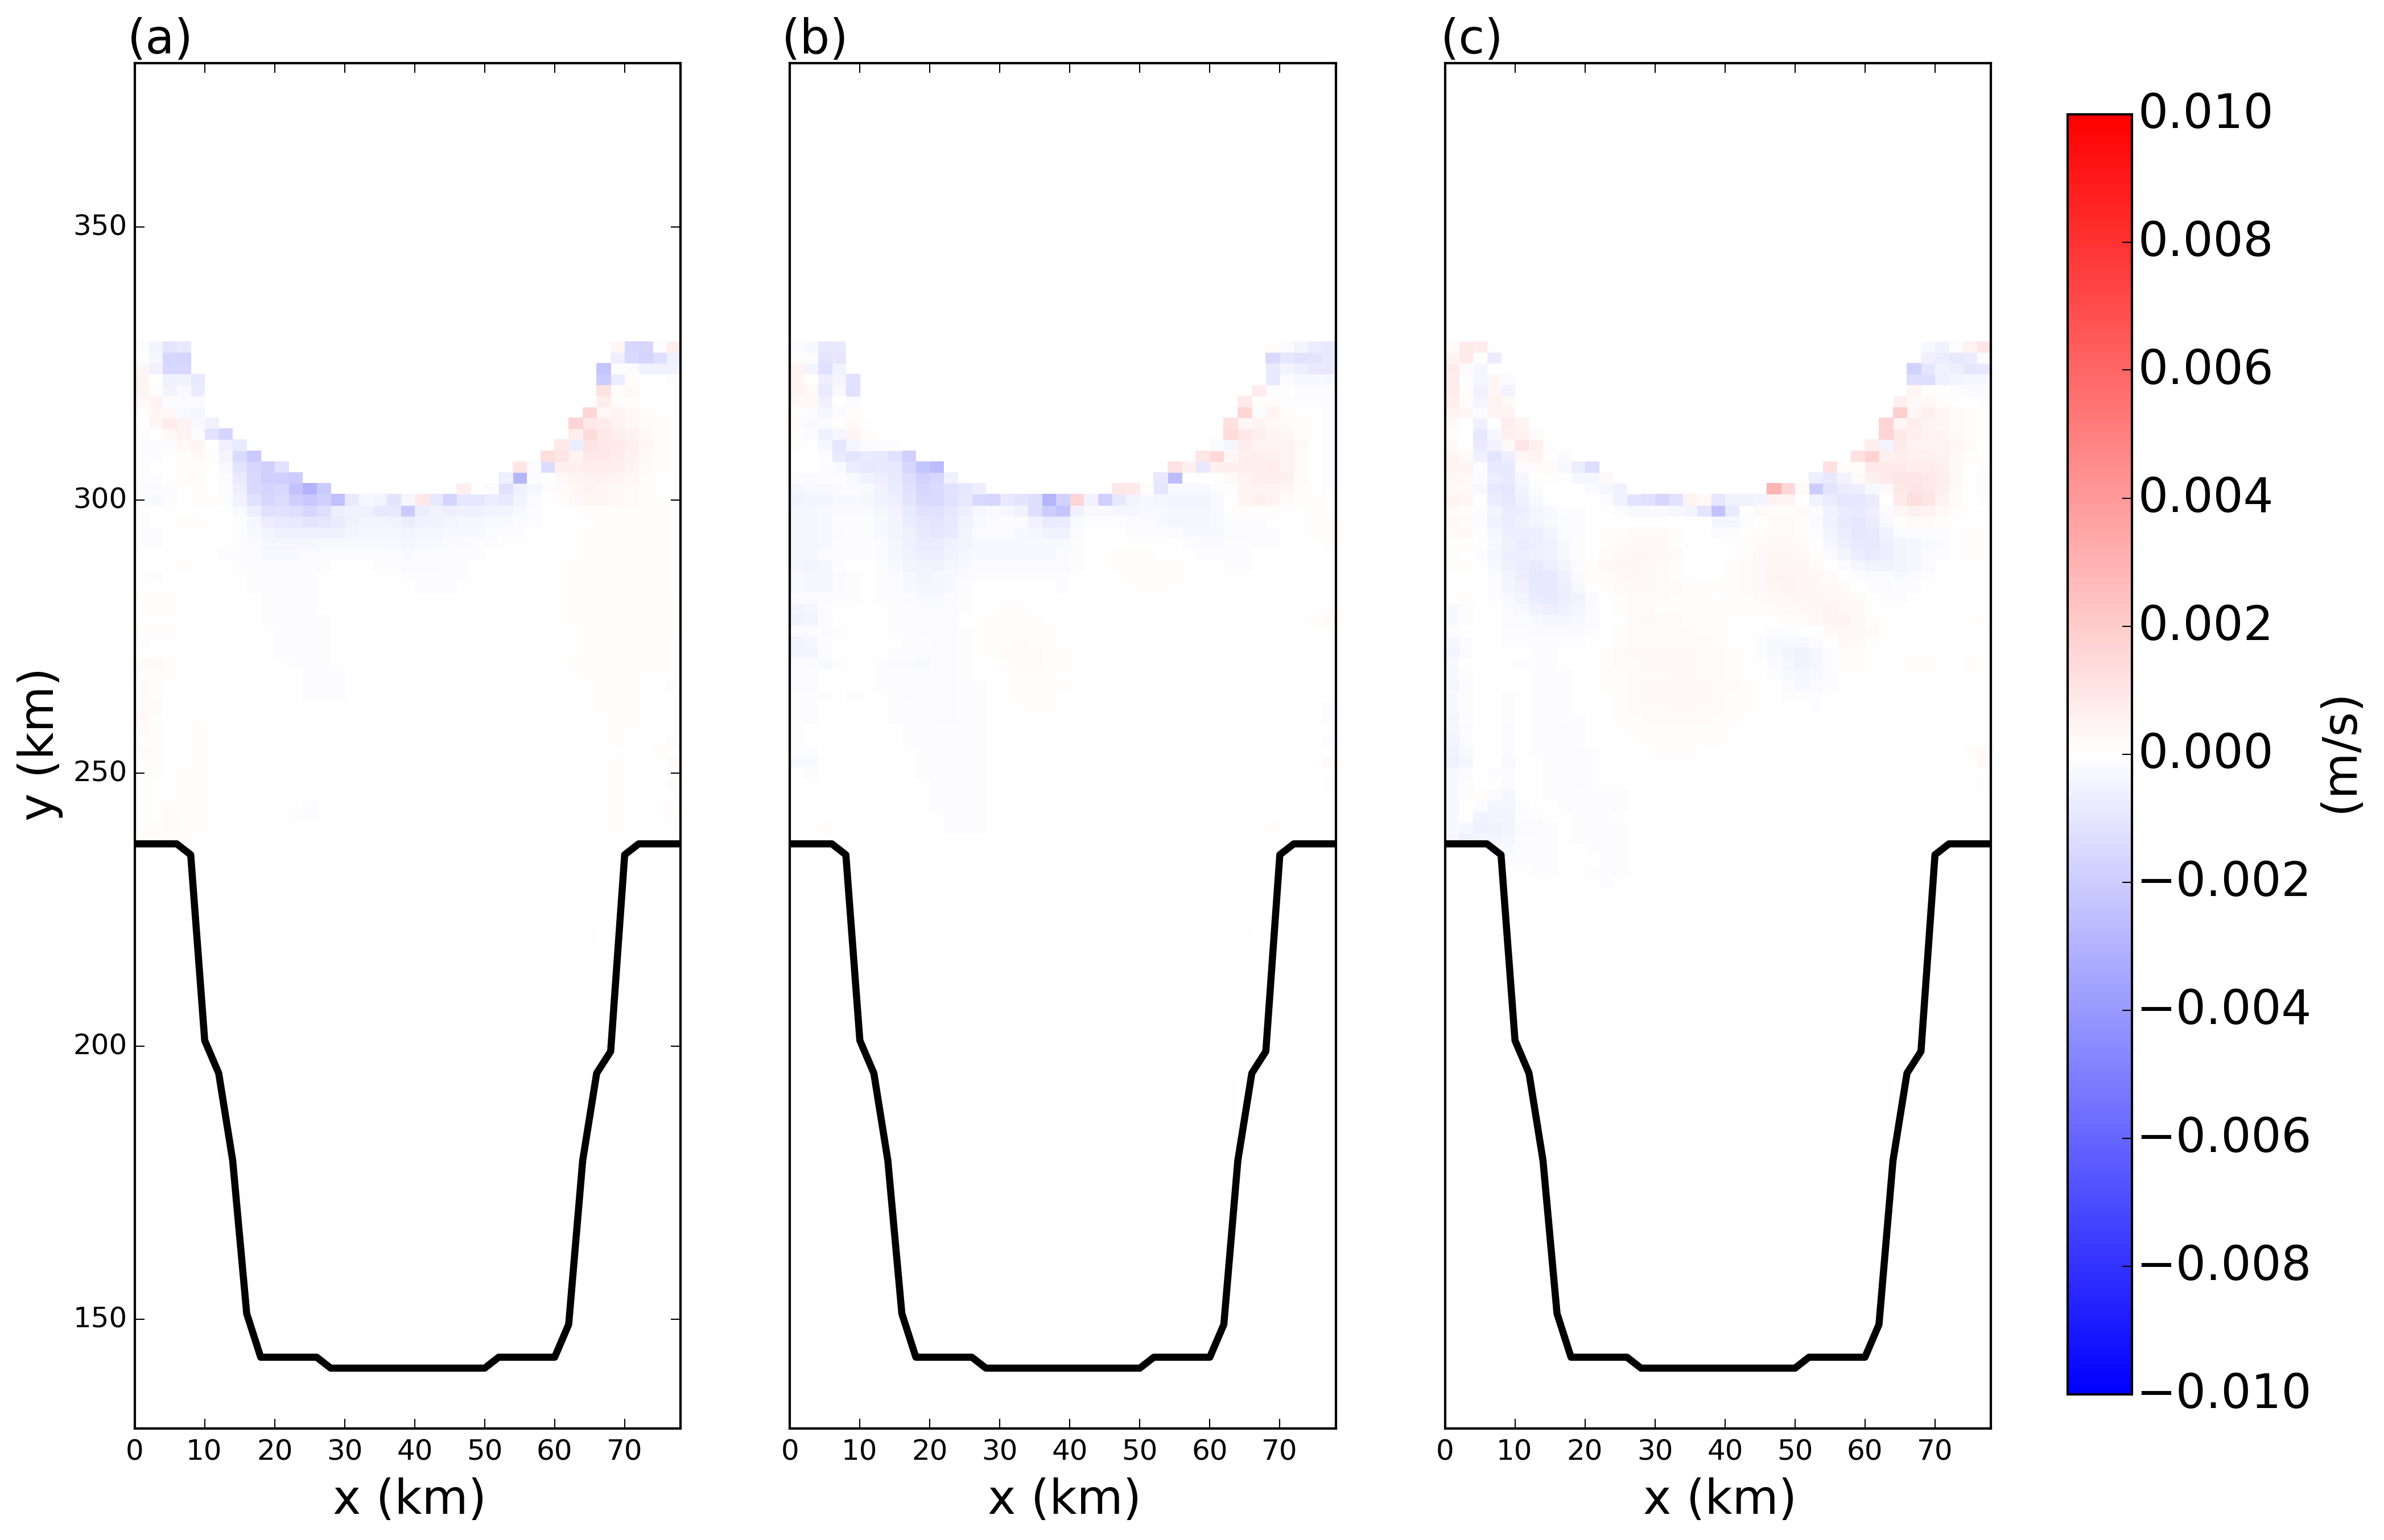
\includegraphics[width=0.99\textwidth]{Figures/snapshots_Wind_Wind_Collapse_ustar_iceberg.png}
%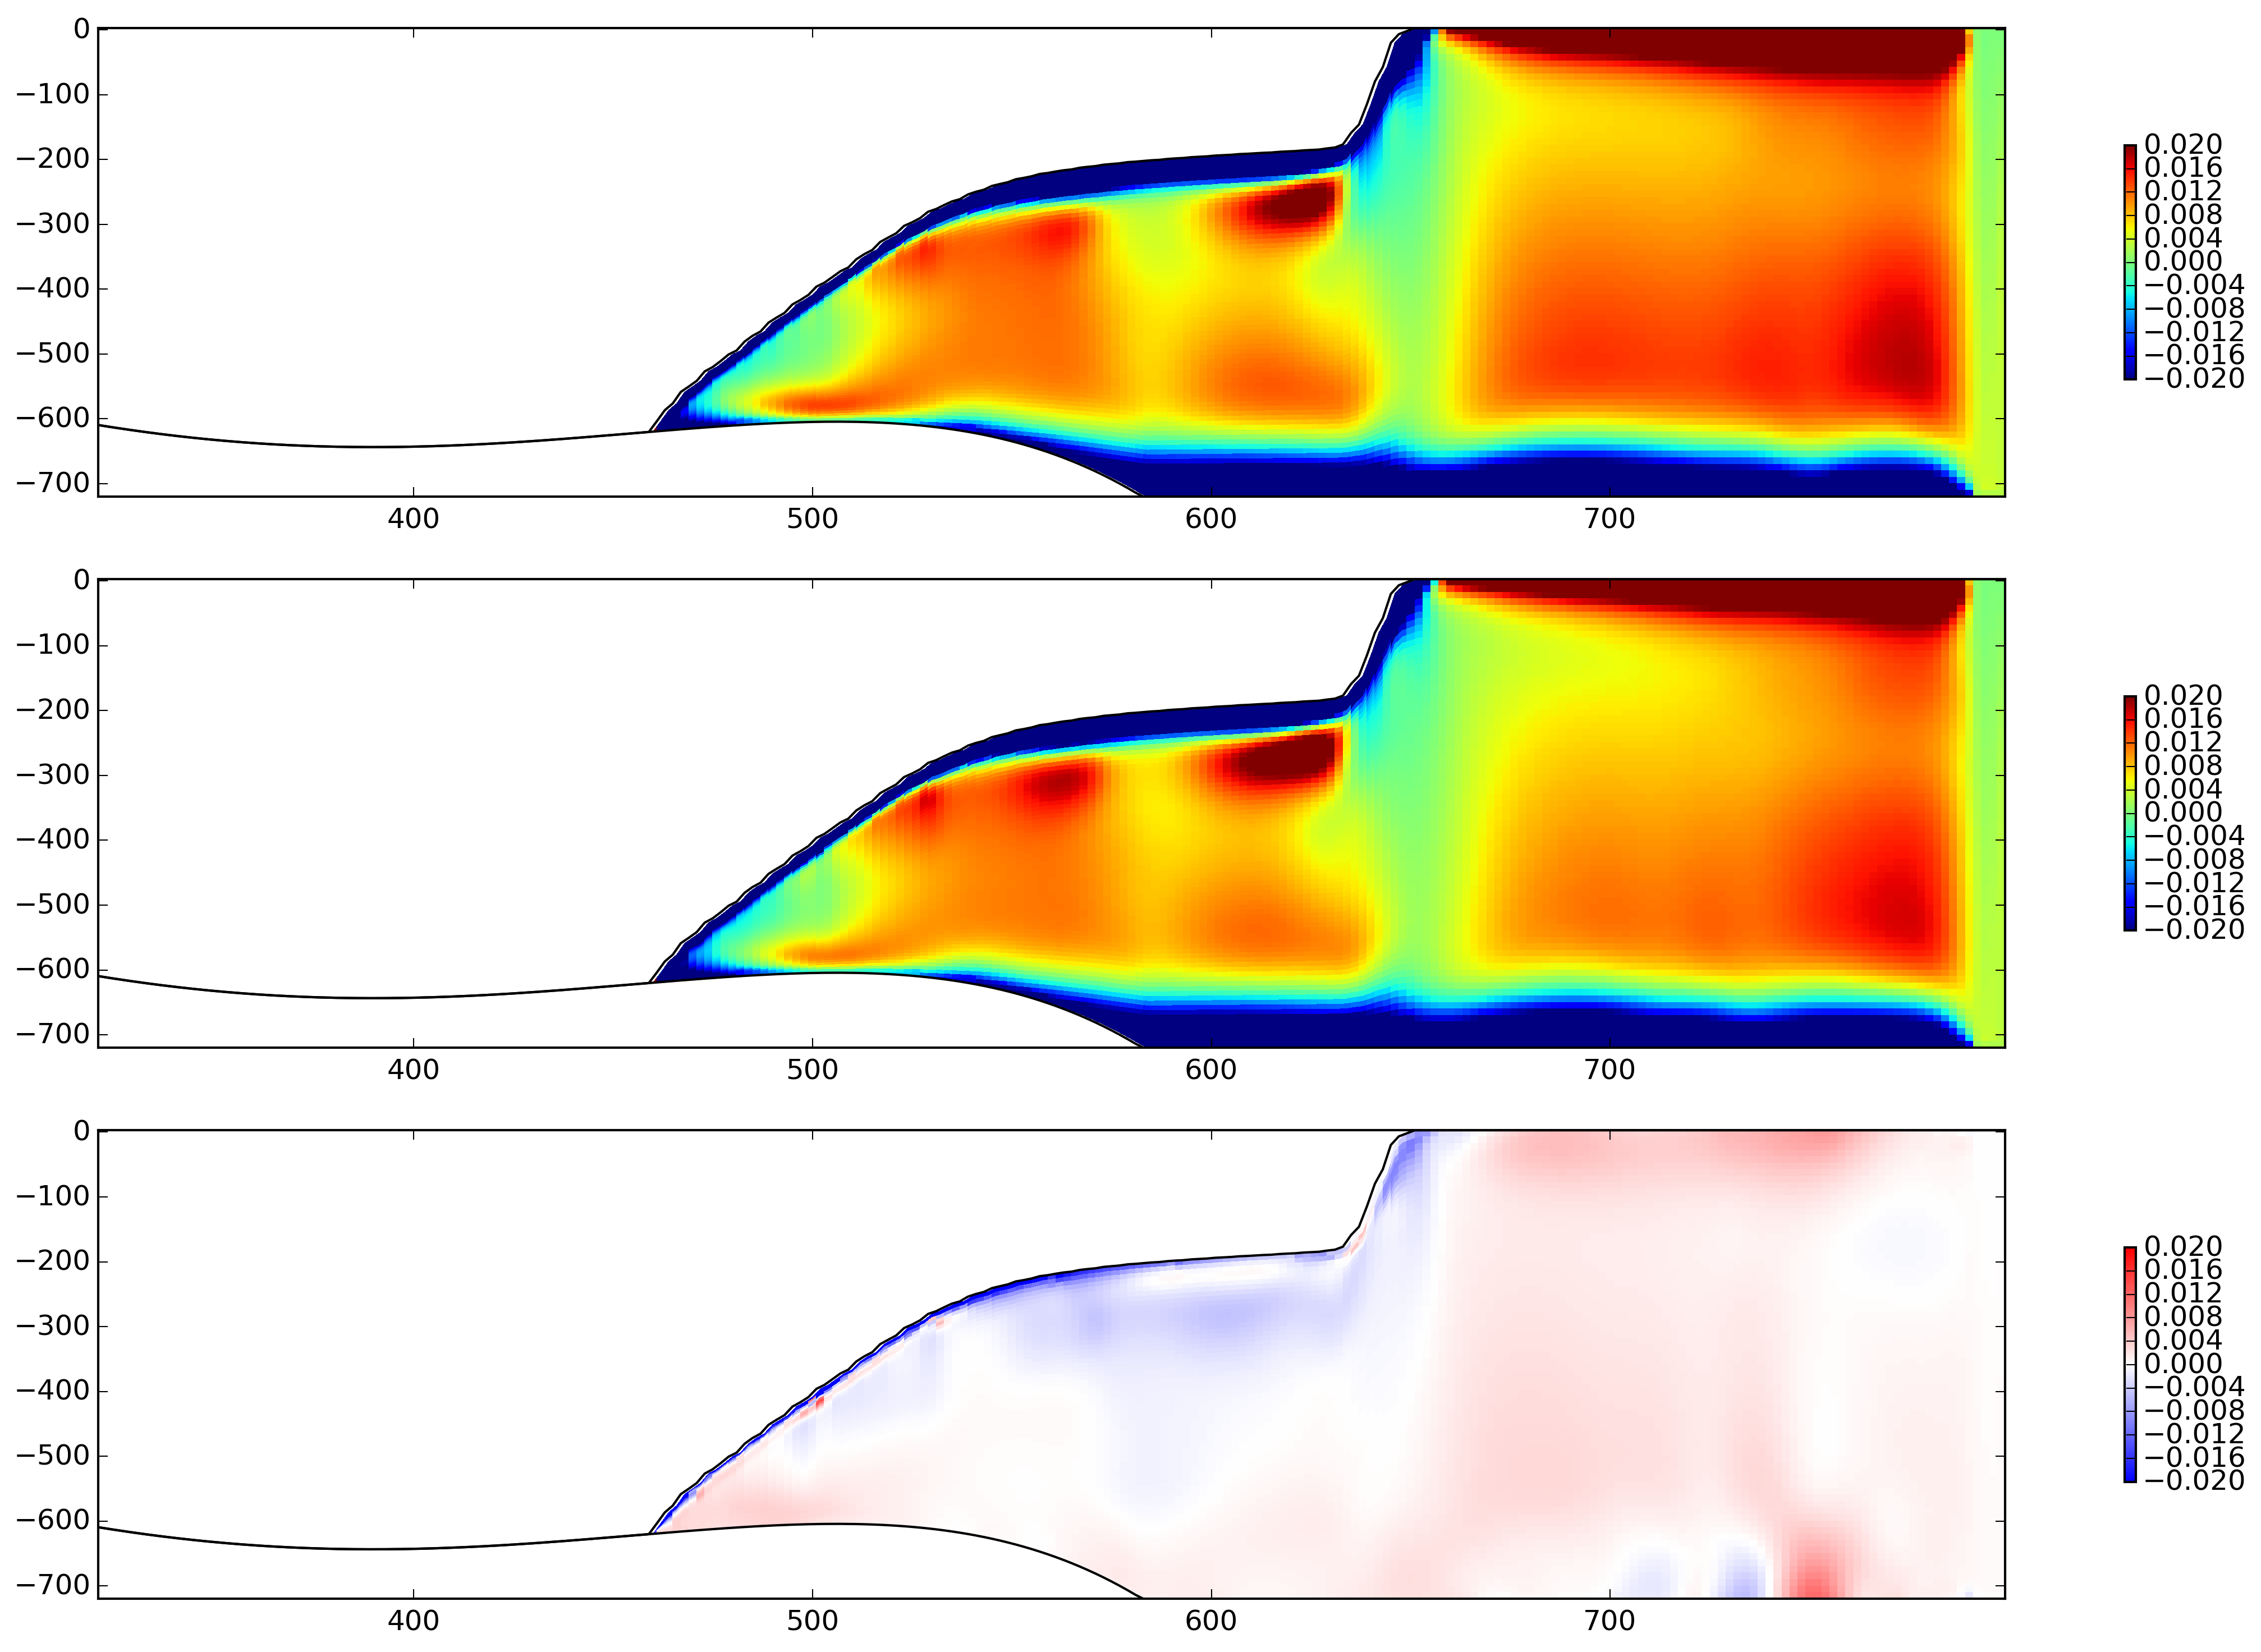
\includegraphics[width=0.99\textwidth]{Figures/ALE_z_static_shelf_comparison_salt_layers.png}
\caption{ {Snapshots of frictional velocity at the ice-shelf base in the tabular-iceberg-calving simulation. Snapshots are taken (a) 7, (b) 15, and (c) 50 days after calving.}}
\end{center}
\label{fig:ustar_calving}
\end{figure}
 \clearpage
    
  
  
  

\begin{figure}
\begin{center}
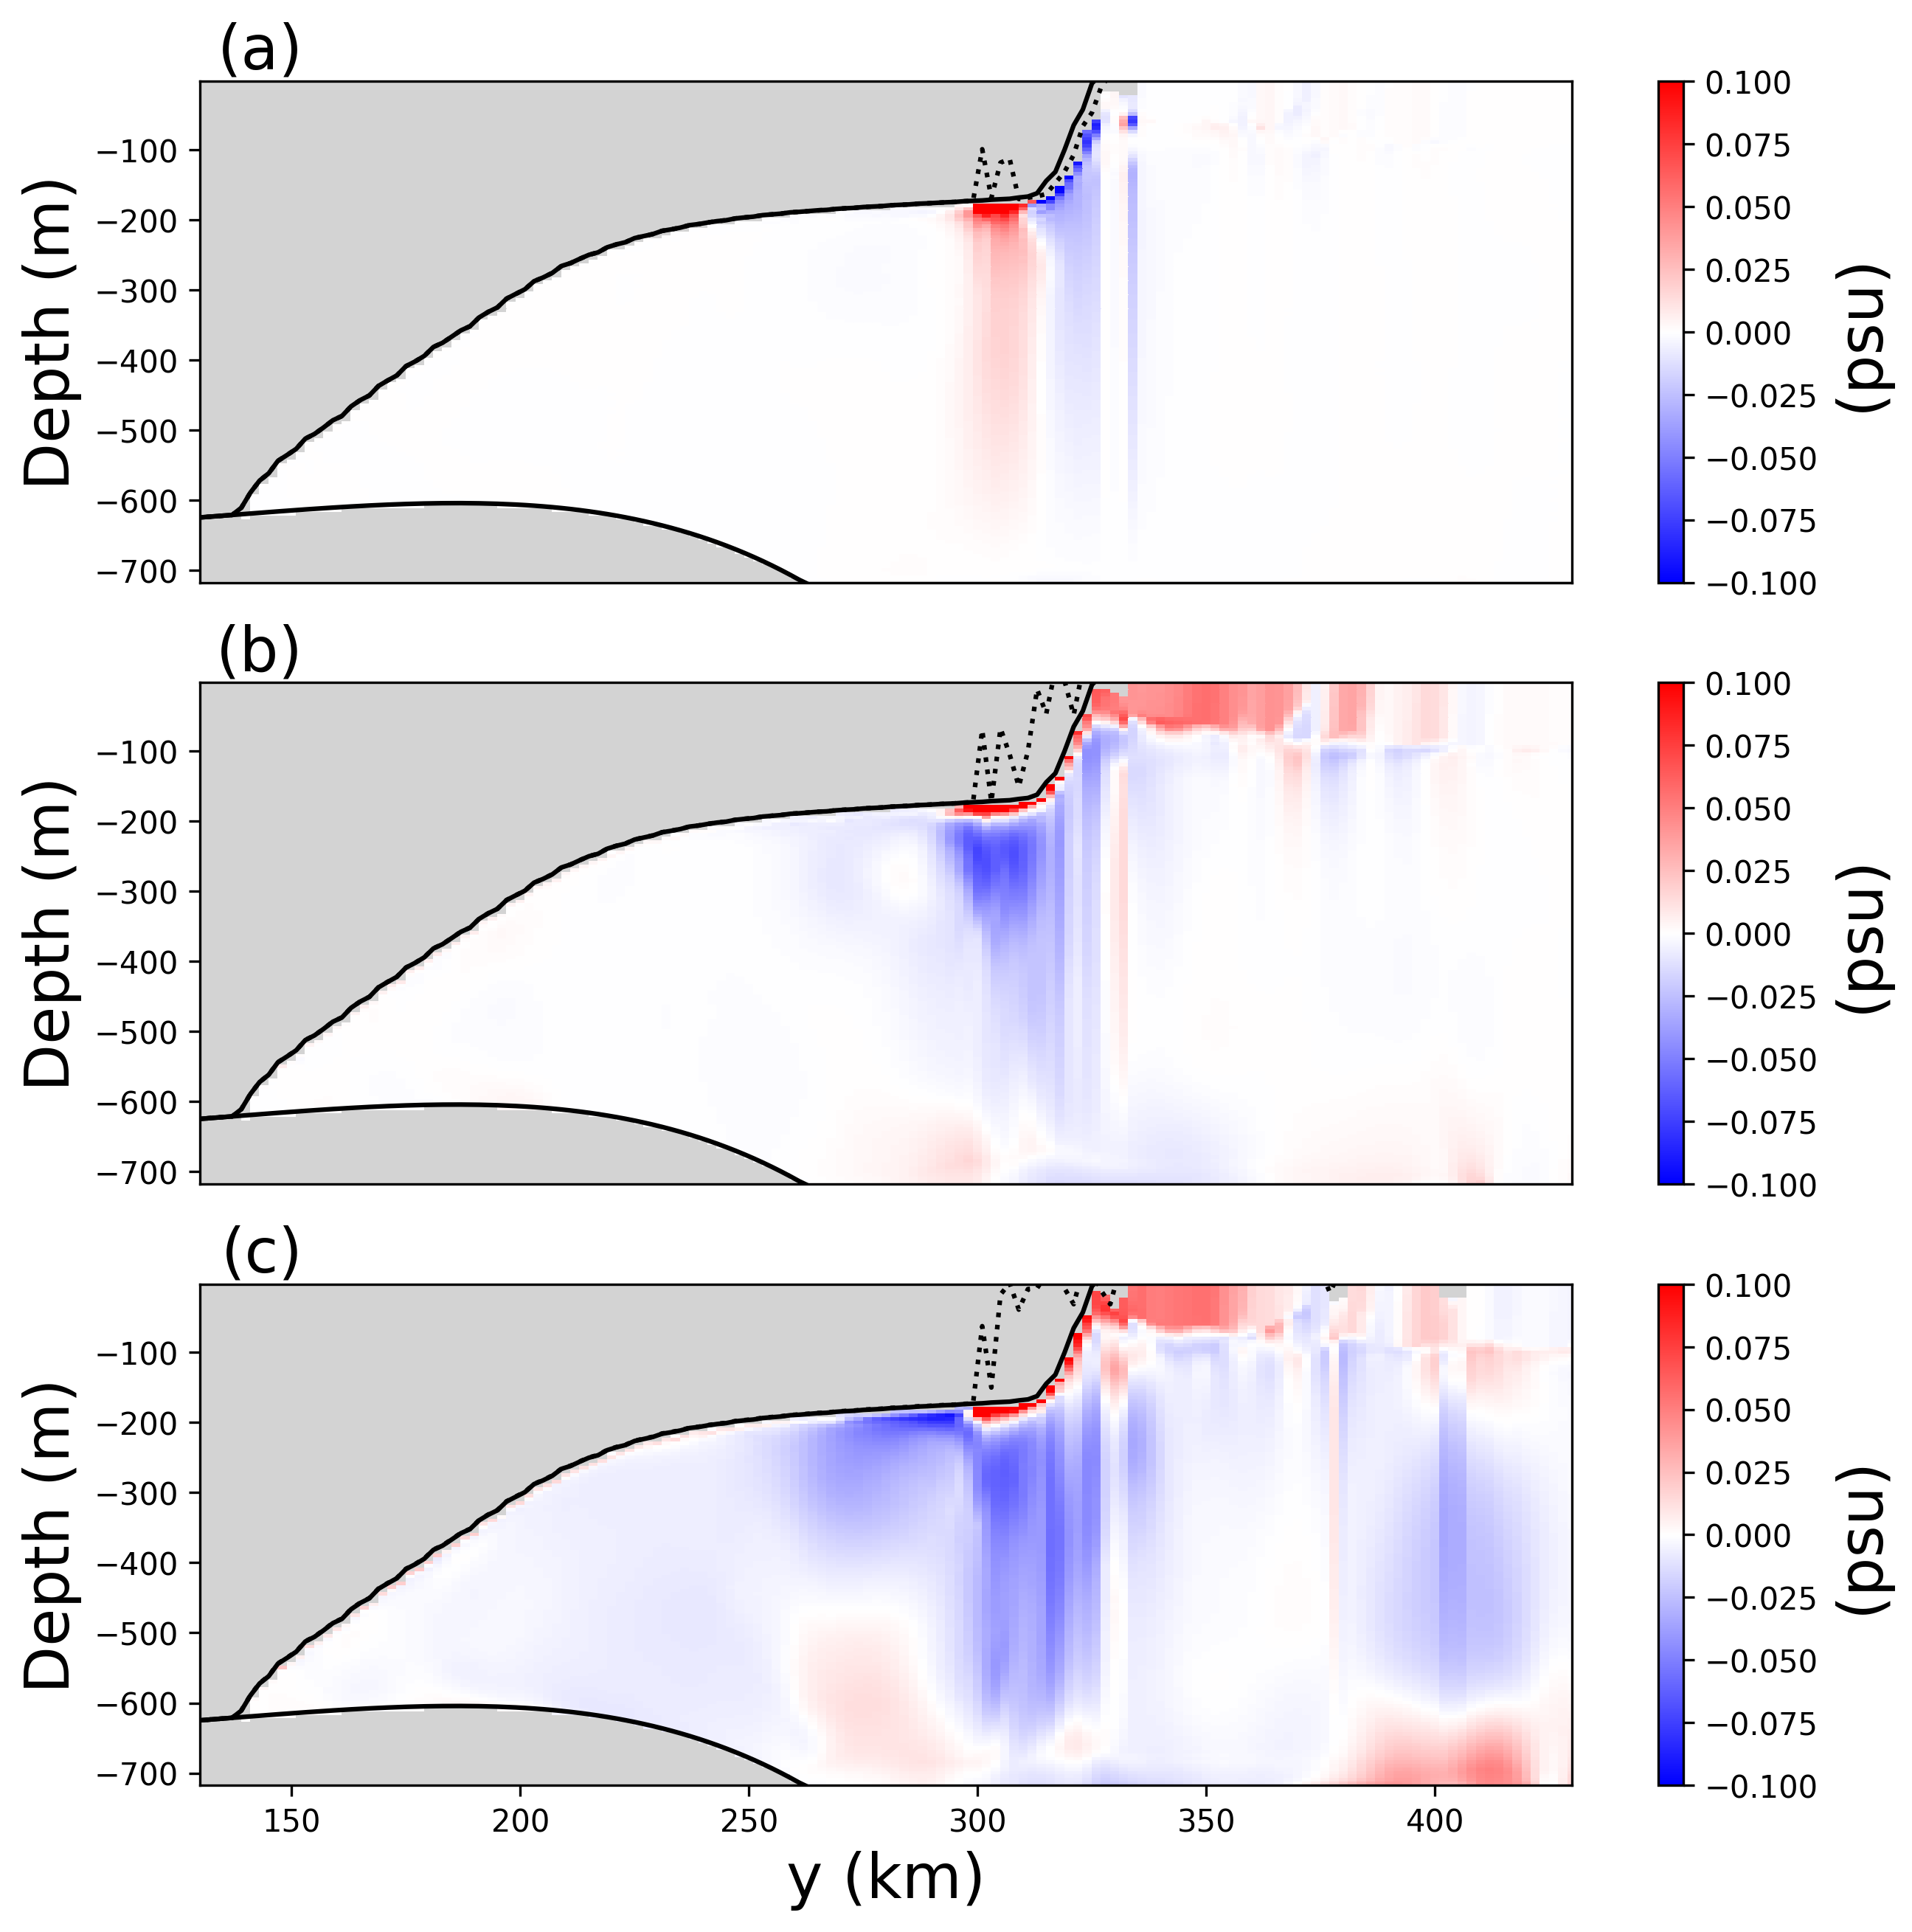
\includegraphics[width=0.99\textwidth]{Figures/snapshots_Wind_Wind_Collapse_salt_zold_x20_anomaly_mask.png}
%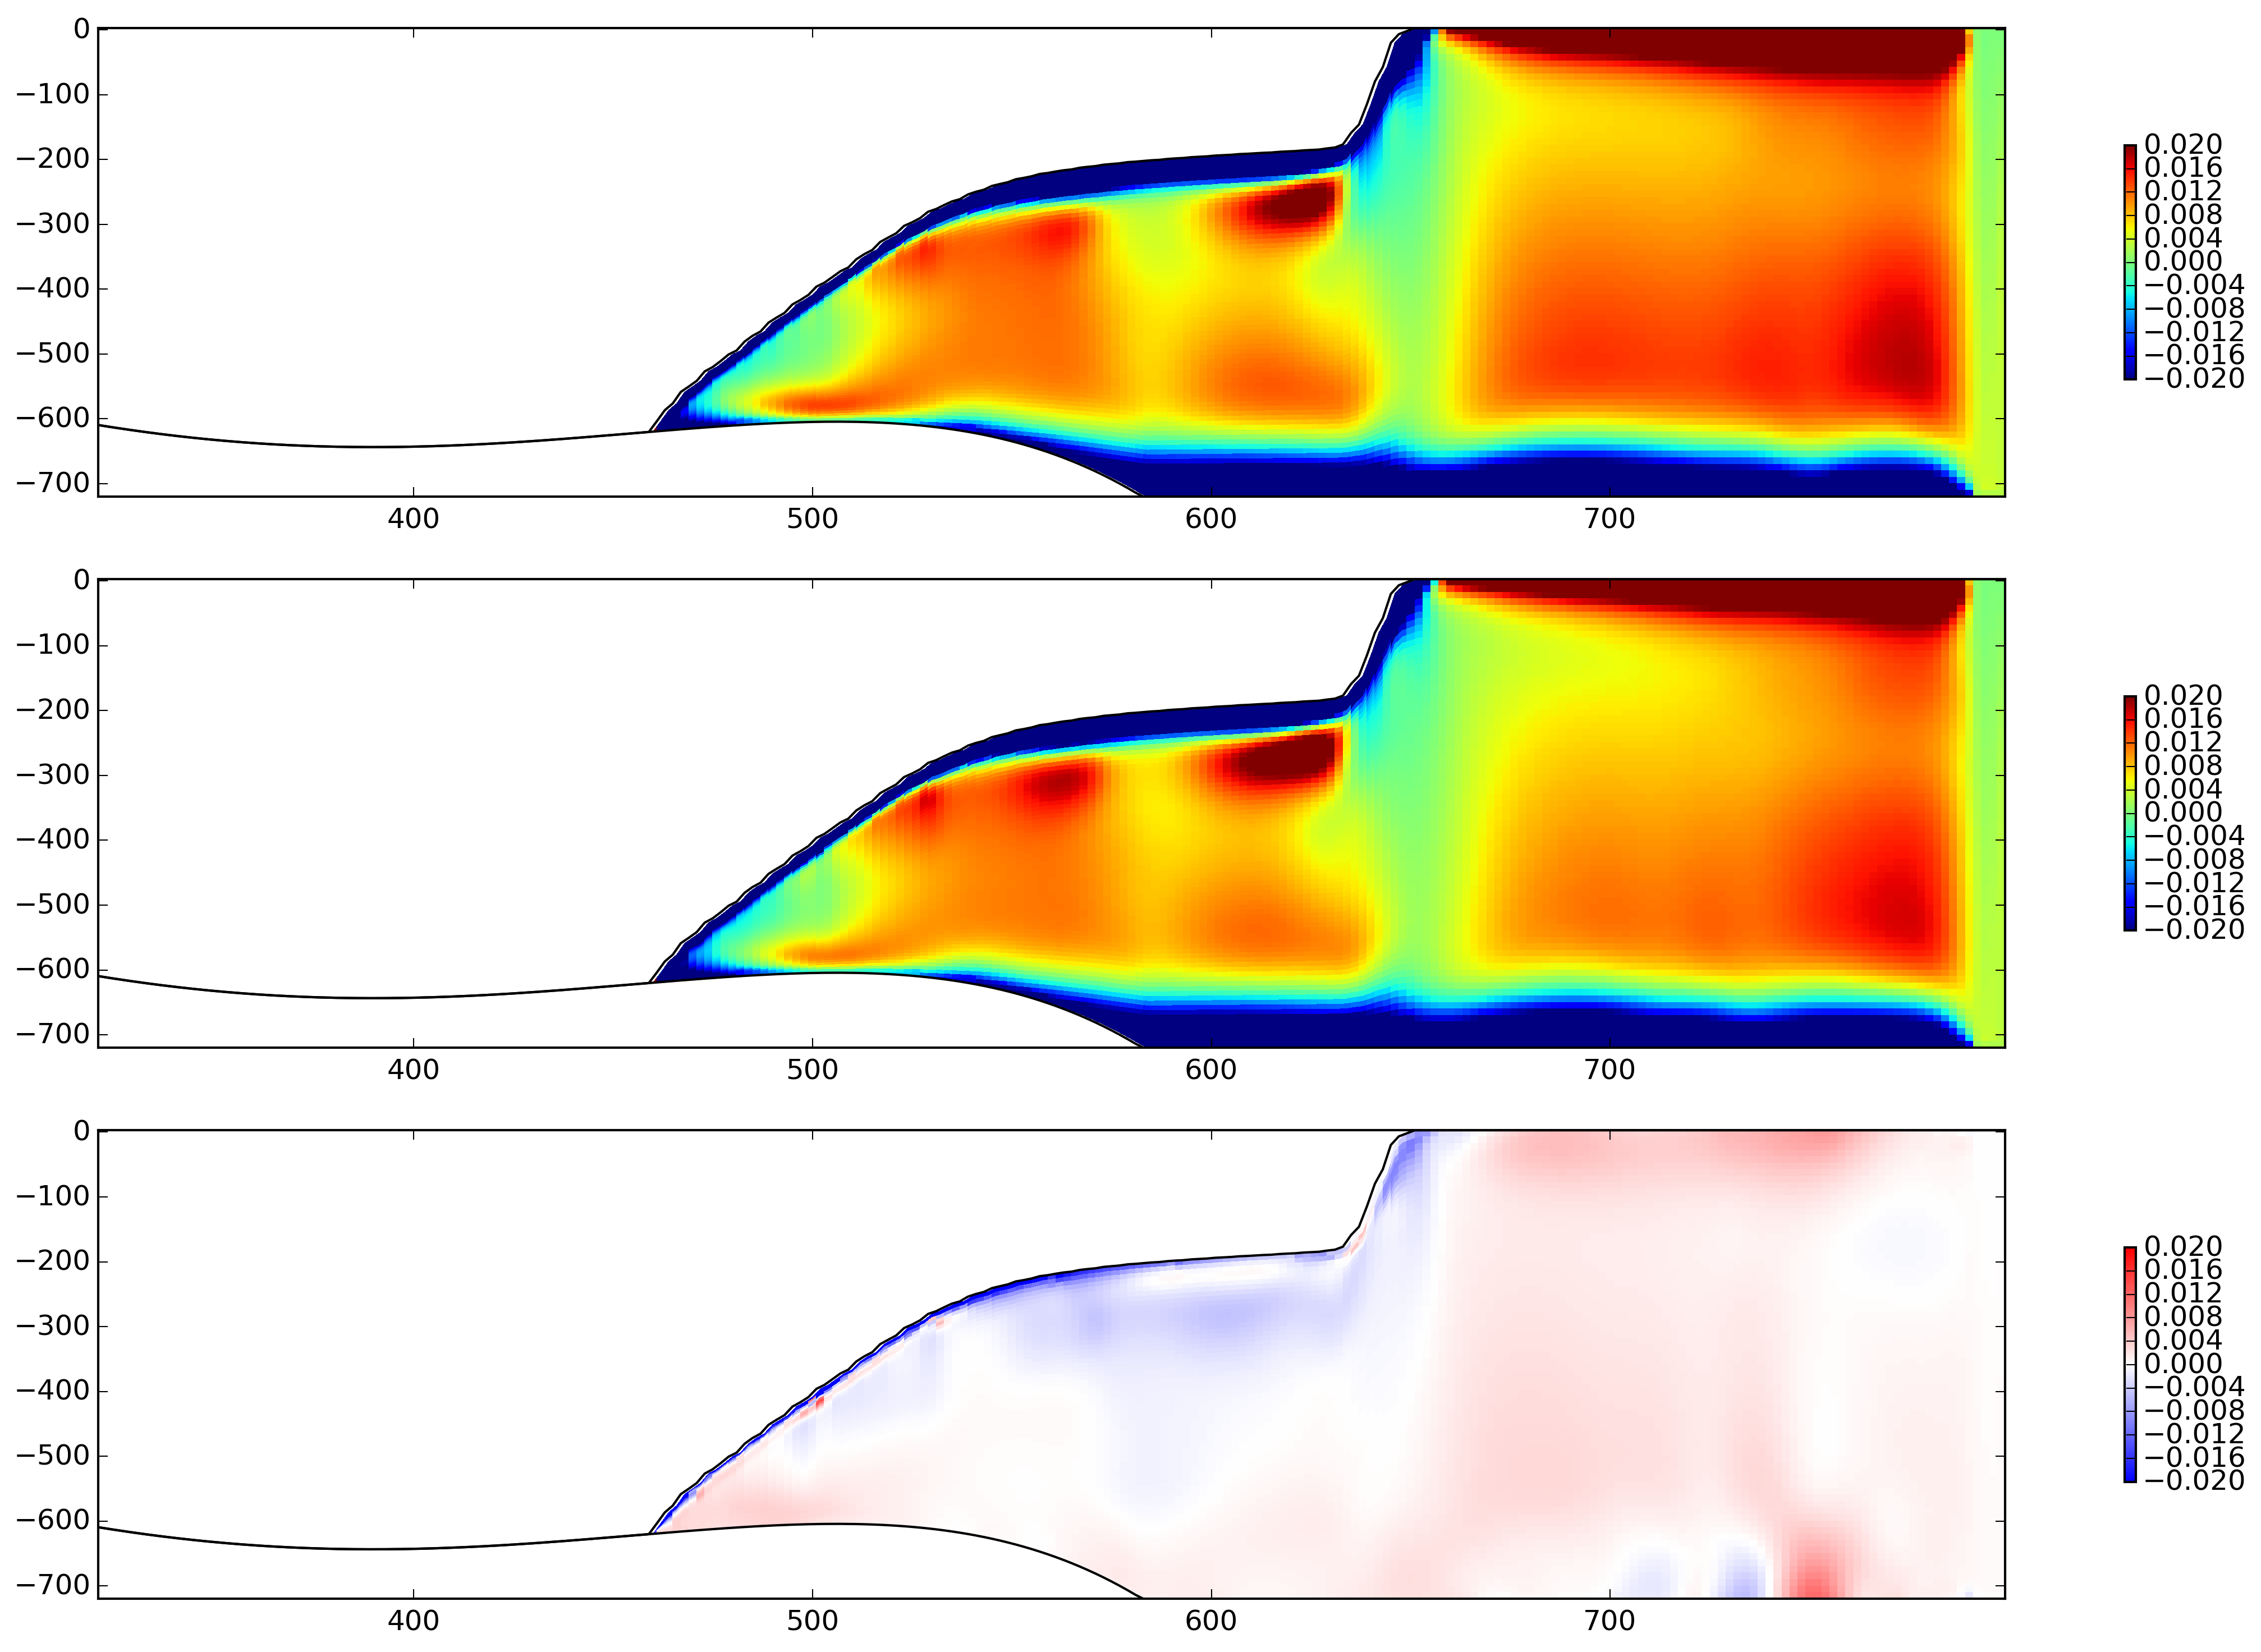
\includegraphics[width=0.99\textwidth]{Figures/ALE_z_static_shelf_comparison_salt_layers.png}
\caption{ {Snapshots of vertical sections of ocean salinity anomaly at $x$=40~km in the iceberg-calving experiment. The anomalies are relative to pre-calving temperatures. Snapshots are taken (a) 1, (b) 15, and (c) 50 days after calving. In each panel, the base of the ice before calving and at the time of the snapshot are shown by the solid and dashed black lines, respectively. Positions that were not the ocean interior at in both snapshots are masked in grey. The position of the vertical transects is shown by the black dashed lines in Figure \ref{fig:SST_snapshots}a.}}
\end{center}
\label{fig:Salinity_section_Collapse_yz}
\end{figure}
 \clearpage




  
   
   

 

 \end{document}

%%%%%%%%%%%%%%%%%%%%%%%%%%%%%%%%%%%%%%%%%%%%%%%%%%%%%%%%%%%%%%%

